\documentclass[]{final_report}
\usepackage{graphicx}

\usepackage{titlesec}
\usepackage[utf8]{inputenc}
\usepackage[backend=biber, style=ieee]{biblatex}
\usepackage{amsmath}
\usepackage{amssymb}
\usepackage{float}
\usepackage{tabularx} % Needed for the X column type
\usepackage{booktabs} % For prettier tables
\usepackage{lipsum}   % For dummy text
\usepackage{mathtools}
\usepackage{stmaryrd}
\usepackage{mdframed}
\usepackage{caption}
\usepackage{array}
\usepackage{listings}
\usepackage[dvipsnames]{xcolor}
\usepackage{adjustbox}
\usepackage{tikz}
\usepackage{rotating}
\usepackage{pdflscape}
\usepackage{fancyhdr}
\usepackage{comment}
\usepackage{array}
\usepackage{multirow}
\usepackage{tcolorbox} 
\usepackage{pdflscape}
\usepackage{lscape} % Use lscape package instead of pdflscape
\usepackage{afterpage} % Required for \afterpage command
\usepackage{fancyhdr} % Required for custom headers and footers
\usepackage{everypage}
\usepackage{lipsum}
\usepackage{url}
\usepackage{longtable}






\addbibresource{fyp.bib}
\usepackage{amsthm}


\theoremstyle{definition}
\newtheorem{definition}{Definition}[chapter]
\newtheorem{basic}{Basic Definition}
\newtheorem{theorem}{Theorem}
\newtheorem{implication}{Implication}

% Define the Java code style
\lstdefinestyle{mystyle}{
    language=Java,
    commentstyle=\color{OliveGreen},
    keywordstyle=\color{blue},
    numberstyle=\tiny\color{gray},
    stringstyle=\color{red},
    basicstyle=\ttfamily\footnotesize,
    breakatwhitespace=false,         
    breaklines=true,                 
    captionpos=b,                    
    keepspaces=true,                 
    numbers=left,                    
    numbersep=5pt,                  
    showspaces=false,                
    showstringspaces=false,
    showtabs=false,                  
    tabsize=2
}
\lstset{style=mystyle}

% Define the landscape page number command
\newcommand{\Lpagenumber}{%
  \ifdim\textwidth=\linewidth
    \else
      \bgroup
      \dimendef\margin=0 %use \margin instead of \dimen0
      \ifodd\value{page}
        \margin=\oddsidemargin
      \else
        \margin=\evensidemargin
      \fi
      \raisebox{\dimexpr -\topmargin-\headheight-\headsep-0.5\linewidth}[0pt][0pt]{%
        \rlap{\hspace{\dimexpr \margin+\textheight+\footskip}%
        \llap{\rotatebox{90}{\thepage}}}}%
      \egroup
  \fi
}
\usepackage{hyperref}
% Add the page number command to every page
\AddEverypageHook{\Lpagenumber}
\newcommand{\mycomment}[1]{}
%%%%%%%%%%%%%%%%%%%%%%
%%% Input project details
\def\studentname{Jude Asare}
\def\reportyear{2023/2024}
\def\projecttitle{Implementing the PKCS\#1 v1.5 and other deterministic RSA Signature Schemes with provably secure parameters}
\def\supervisorname{Saqib Kakvi}
\def\degree{MSci (Hons) in Computer Science (Information Security)}
\def\fullOrHalfUnit{MSci} 
\def\finalOrInterim{Final Report} 
\begin{document}

\maketitle


%TC:ignore

\pagenumbering{roman} % Start with Roman numerals


\chapter*{Declaration}

This report has been prepared on the basis of my own work. Where other published and unpublished source materials have been used, these have been acknowledged.

\vskip3em

Word Count: 17565
\begin{itemize}
\item Includes a section on professional issues.
\item Excludes the appendix (optional for perusal) which contains full documentation of requirements, design, testing, and remaining results tables.
\end{itemize}
\vskip3em

Student Name: \studentname


\newpage

%TC:endignore




%%%%%%%%%%%%%%%%%%%%%%
%%% Table of Contents
\tableofcontents\pdfbookmark[0]{Table of Contents}{toc}\newpage



%%%%%%%%%%%%%%%%%%%%%%
%%% Your Abstract here
\begin{comment}
\mycomment{

\begin{abstract}



The PKCS\#1 v1.5 digital signature scheme has been widely utilised in protocols such as SSH, DNSSEC, IKE, and most prominently, in TLS up to version 1.2. Since its inception in 1998 \cite{rfc2313} it has played a pivotal role in the landscape of digital security comprising the most widely used digital signature scheme in practice. The scheme, renowned for its straightforwardness and expedited verification capabilities, has seen persistent integration across diverse cryptographic systems. 

Nevertheless, amidst its widespread acceptance, it's been marred by several challenges. Among these are the targeting of a latent vulnerability with incorrectly implemented signature verification implementations \cite{finney2006bleichenbacher, kuhn2008variants, bock2018return} stemming from attacks \cite{bleichenbacher1998chosen} exploiting its provably insecure associated encryption paradigm \cite{rfc2313} and a glaring absence of a rigorous security proof that validates its robustness.

Even though alternatives like RSA-PSS offer provable security (\cite{bellare1996exact}, \cite{jonsson2001security}), they come with inherent problem, such as the introduction of randomness and a hike in computational complexity. These issues have created reservations for its wholesale adoption in place of PKCS\#1 v1.5 e.g., RSA-PSS and was only upgraded to a requirement for new applications in PKCS\#1 v2.2 \cite{rfc8017} long after initially being suggested as the replacement for PKCS\#1 v1.5 in PKCS\#1 v2.1 \cite{rfc3447}. Imperative requirements of backward compatibility and interoperability have been the main detractors of the aversion to replacing PKCS\#1 v1.5 and while RSA-PSS is now required in new applications, they entail retaining PKCS\#1 v1.5 in some form at the very least, as a preferable choice.
 
A significant breakthrough came in 2018 when Jager, Kakvi, and May \cite{jager2018security} provided a security proof for the PKCS\#1 v1.5 Signature scheme building on the work of Coron \cite{coron2002security}. Although still requiring the adoption of larger cryptographic parameters deviating slightly from standard use, their methods were flexible enough to show instantiations in practice such that the improved proofs apply. Benefits not limited to PKCS\#1 v1.5, their work also offered insights enabling the proof to apply to other deterministic RSA signature schemes, with similar construction patterns including ISO/IEC 9796-2 and ANSI X9.31 schemes.

Guided by this revelation, this project seeks to concretely implement these signature schemes, with a primary emphasis on the PKCS\#1 v1.5 signature scheme, using the aforementioned provably secure parameters. This project primarily aims to dissect the burden on computational these parameters introduce into deterministic RSA schemes. This aim is supplemented by supporting objectives to produce algorithms that facilitate implementation of the schemes with provably secure and standard parameters. From there the main objective is to produce a user-interfaced benchmarking program to explore aforementioned overhead across various key sizes for the different deterministic signature schemes. 
\newpage
\end{abstract}
}
\end{comment}
\newpage

\pagenumbering{arabic}
%%%%%%%%%%%%%%%%%%%%%%
%%% Introduction

\chapter{Introduction}


\section{Aims}

\subsection{Why: The Context and Rationale}
The PKCS\#1 v1.5 digital signature scheme, rooted in RSA's hash-and-sign framework, has emerged as the de facto standard for digital signatures since its 1998 introduction \cite{rfc2313}. Essential in security-focused network protocols like SSH, DNSSEC, IKE, and pre-TLS 1.3 X.509 certificates \cite{schaad2005additional}, its simplicity fostered broad adoption from its outset with a straightforward implementation across programming languages, and speedy verifications relative to alternatives like DSA or ECDS  \cite{jager2018security}. 
Despite its widespread adoption the scheme lacks formal security proofs, raising concerns about its long-term reliability.
Given its deep integration in various applications, even at the hardware level, transitioning to provably secure \cite{bellare1996exact, jonsson2001security} alternatives like RSA-PSS has been slow (RSA-PSS was only upgraded to a requirement for new applications in PKCS\#1 v2.2 \cite{rfc8017} long after initially being suggested as the replacement for PKCS\#1 v1.5 in PKCS\#1 v2.1 \cite{rfc3447}) with imperative requirements of backward compatibility and interoperability acting as significant barriers to full adoption.

Additionally considered in a broader sense, for a cryptographic scheme i.e., RSA-PSS to gain traction it must first be developed and then subjected to rigorous scrutiny by the cryptographic community. Following this, its algorithmic primitives need to be standardised, which then facilitates the creation and standardisation of high-level protocols incorporating these components. Subsequent software implementations must align with these standards before the scheme can be set as the default in various applications. RSA-PSS, while superior to the older PKCS\#1 v1.5 lingers in the early stages of this transition mainly between standardisation of its algorithm primitives and the standardisation of protocols that incorporate its primitives. The current landscape is one of fragmentation where RSA-PSS and PKCS\#1-v1.5 often coexist within the same infrastructure, such as TLS implementations and RSA certificates. This state of the art considered, retaining PKCS\#1 v1.5 scheme remains a preferable choice. Going even further, finding an applicable security proof to bridge its security to the level of its widespread adoption would be the ideal scenario.

In this direction a landmark development came in 2018 when Jager, Kakvi, and May \cite{jager2018security} provided a security proof (an improvement on Coron's proof that was limited to the Rabin-Williams variant with e=2 \cite{coron2002security}) for the PKCS\#1 v1.5 signature scheme, with a caveat: usage of larger parameters are required. Their work offered insights that also apply to other deterministic (and standardised) RSA signature schemes, including ISO/IEC 9796-2 Scheme 1 and ANSI X9.31 rDSA.

\subsection{What: The Primary Goal}
The aim of this project was to connect the theoretical concepts introduced by Jager et al. \cite{jager2018security} with practical application. This involved implementing provably secure parameters and then assessing the burden on computational time that arises when using them in deterministic RSA signature schemes.

\subsection{How: Overview of Objectives}
The project pursued a methodical approach to assess the impact on computational time of employing provably secure parameters in deterministic RSA signature schemes. This was achieved by developing algorithms respective to both cases (standard vs. provably secure parameters) and comparing them for various key sizes when applied to large batches of data (in the case of signature operations) or in the case of key generation, generating keys repeatedly for each parameter type at scale.
The investigation spanned across various signature scheme standards as means of enhancing the reliability and accuracy of the findings by offering views into the computational overhead from within the context of different schemes. The final deliverable constituted an all-incorporative user-interfaced benchmarking program for which results from each of the signature schemes working on batches of data for multiple key sizes were generated.

\subsection{Overview of Results}
Overall, the results indicated that the integration of provably secure parameters into deterministic signature schemes, far from being a computational burden, can rather lead to substantial improvements in verification times (hash function dependent), while there is no observed impact on signature creation. In terms of key generation, the impact varies based on whether the focus is on the use of smaller exponent values ('e') or the inclusion of additional primes. While smaller 'e' values show minimal effects, the introduction of a third prime factor notably enhances key generation efficiency across all key sizes.




\section{Objectives}
To achieve the aim, the project involved:
\begin{itemize}
    \item Exploring the security proof relevant to the PKCS\#1 v1.5 signature scheme .
    \item Determining the practical implications arising from the security proof on instantiations of the full suite of deterministic signature schemes (PKCS\#1-v1.5, ISO/IEC-9796-2, and ANSI-X9.31 signature schemes).
    \item Developing concrete implementations of the considered deterministic signature schemes using standard and provable parameters.
    \item Demonstrating in practice, with larger parameters, how deterministic schemes can achieve a security level on par with less-practical, signature schemes, such as RSA-PSS.
      \item Evaluating and comparing computational time of instantiating the considered signature schemes with standard vs. provable parameters. 
     \item Creating a user-interfaced benchmarking program that incorporates all objectives of the project to assess the overhead across various key sizes for the different deterministic signature schemes.

\end{itemize}



\begin{comment}
Key Generation results indicated use of provably secure parameters marginally impacts the efficiency of key generation positively at lower key sizes with the effect dissipating with increase in key size. Signature creation results indicated negligible performance between standard and provably secure parameters across all tested schemes. Signature verification results indicated significant improvement in times when using provably secure parameters as compared to standard parameters. This enhancement, however, varied depending on the security level of the hash function. 
\end{comment}

\section{Organisation}
The structure of this paper is outlined as follows: Chapter 2 presents related work on the provable security of deterministic schemes. Chapter 3 covers the background theory for RSA signature schemes. Chapter 4 discusses the proof theorems and draws out their practical implications. Chapter 5 explores assumptions used in implementation, these being derived from the implications presented in Chapter 4. Chapter 6 details the complete development of the project's deliverable. Chapter 7 presents the results, coupled with summaries of key findings. Finally, Chapter 8 concludes the paper with a synthesis of the discussed points.


\chapter{Literature Review/Related Work}
RSASSA-PKCS1-v1.5 remains unbroken. There are no real attacks able to successfully exploit the scheme free of implementation errors. This distinction of being free of implementation errors is crucial. Potential proofs consider only forgeries that are accepted by a correct verification algorithm. It is now well established from a variety of follow up studies all originating from \cite{bleichenbacher1998chosen} that vulnerable implementations of a flawed signature verification algorithm for RSASSA-PKCS1-v1.5 can be exploited. Bleichenbacher presented a low-exponent attack on RSA-PKCS\#1 v1.5 signatures at the CRYPTO 2006 rump session. This attack was later described by Finney \cite{finney2006bleichenbacher} in a posting to the OpenPGP mailing list. 

It was not until the efforts of Coron in 2002 (\cite{coron2002security}) that a security proof applicable to RSASSA-PKCS1-v1.5 arrived. This was due to the issue of deterministic padding scheme that RSASSA-PKCS1-v1.5 uses, rendering standard proof techniques void. Coron presented a security proof for RSASSA-PKCS1-v1.5 (and ISO/IEC 9796-2 signatures) albeit with a restriction that e = 2, i.e. the Rabin-Williams variant \cite{coron2002security} which is secure based on the factoring assumption. 
The proofs' exclusive and/or restrictive value of e aside, a further caveat was that the output size of the hash function needed to be 2/3 the bit length of the modulus N. These restrictions diverge largely from the standard parameters that could potentially be used in the instantiation of RSA-PKCS\#1 v1.5 signatures in practice. 

Much later, Jager, Kakvi and May \cite{jager2018security} showed an improved security proof for RSASSA-PKCS1-v1.5 with less restrictive conditions.
It sufficed that e more generally be a small prime (Kakvi and Kiltz \cite{kakvi2018optimal}). Still requiring a large hash function output, the authors achieved an improvement in hash function output, requiring only 1/2 of the modulus size. The modulus effectively doubles in bit length when compared to the norm with a newly introduced third prime factor necessitating the increase in bits.
Withstanding the improvement and as a consequence of the proofs being founded in the random oracle model, the larger cryptographic parameters still deviate slightly from the standard parameters that could be used in practice. Nonetheless this was sufficient enough for the authors to demonstrate how RSA-PKCS\#1 v1.5 signatures can be instantiated in practice such that the improved proofs apply. 

To all intents and purposes, regardless of the proofs being presented primarily for RSASSA-PKCS1-v1.5, uniformity in construction philosophy means other signature standards of the same deterministic RSA type (ISO/IEC 9796-2 signatures and ANSI X9.31 rDSA) still match the setting required for proofs to be applicable to them. For example theorem statements used in construction of Corons' proof \cite{coron2002security} are general enough that corresponding proof theorems can also be presented for the remaining standards of deterministic signatures. 

A full discussion of provable security extending to non-deterministic schemes lies beyond the scope of this project. Probabilistic padding poses an issue since generating sources of randomness, particularly on constrained devices is an ongoing challenge. Moreover RSA-PSS, the sole RSA-based randomised digital signature scheme uses two hash functions. This makes it difficult to compare with deterministic schemes that use only one. This project focused on standardised deterministic schemes which are directly comparable and subversion resistant \cite{ateniese2015subversion} by default of not having to generate randomness. This lends well to the issue of examining computational overhead from various perspectives of the different deterministic standards.



\chapter{Cryptographic Foundations}
\section{Notations}
The security parameter is denoted as \( \lambda \). 
This parameter determines a system's security level or key sizes. A larger value of $\lambda$ indicates stronger security, though it requires more computational effort. The concept of binary strings is frequently referred to. Specifically for all \( n \in \mathbb{N} \), the symbol \( 1^n \) represents the n-bit string of consecutive ones. 

In cryptographic operations, sampling often involves randomness. Given any set \( S \), the notation \( x \in_{R} S \) signifies that \( x \) is chosen uniformly at random from \( S \).  
The set of prime numbers is represented as \( \mathbb{P} \) and the set of \( k \)-bit primes is denoted as \( \mathbb{P}[k] \). Similarly, the set of integers is represented by \( \mathbb{Z} \) and \( \mathbb{Z}[k] \) respectively. 

The notation \( \mathbb{Z}_N^* \) represents the multiplicative group modulo \( N \) where \( N \in \mathbb{N} \). 

Finally, game-based proofs are employed, and the notation \( G^A \Rightarrow 1 \) indicates an event where the adversary \( A \) succeeds in game \( G \), specifically when the Finalise Procedure yields an output of 1.


\section{Digital Signature Schemes}
In the realm of security, not every issue revolves around confidentiality. In many instances, the adversaries are not limited to passive surveillance but can be active opponents capable of manipulating or introducing unauthorised messages into a communication stream. In the public key setting, the cryptographic primitive used to provide not only data integrity but also for ensuring the authenticity and non-repudiation of communications is a digital signature scheme. 
Essentially, Digital signatures function as a means of binding an identity to specific information. A signature process consists of transforming the relevant message and the entity’s confidential details to produce tag named a signature. This process serves as a verifiable stamp of authenticity, confirming that the message genuinely originated from the claimed source. Moreover it addresses the concept of non-repudiation. Once a message is signed, the signer is bound to the act of signing and cannot deny having signed a then sent message.

An everyday application of digital signatures is in the domain of web security, specifically in the use of Public Key Infrastructure (PKI) and Certificate Authorities (CAs) for verifying the authenticity of websites. For example, when a user visits a website, the site's digital certificate, issued by a CA, is used to establish a secure connection. The digital signature on the certificate verifies that the certificate is indeed issued by a legitimate Certificate Authority and has not been tampered with. This ensures that the website the user is connecting to is actually the one it claims to be, and not a fraudulent site attempting to impersonate it. 

\begin{definition}
\label{def:digital signature}
A (digital) signature scheme DS consists of three probabilistic polynomial-time algorithms (Gen, Sign, Verify) defined as follows:
\begin{enumerate}
    \item Gen (key-generation algorithm): takes as input the security parameter $1^\lambda$ and outputs a pair of keys $(sk ,vk)$, where $sk$ is the signing key and $vk$ is the verification key.
    \item Sign (signing algorithm): takes as input a private key $sk$, message $m$ and outputs a signature $\sigma$ ($\sigma \leftarrow \text{Sign}_{sk}(m)$).
    \item Verify (deterministic verification algorithm):  takes as input a public key $pk$, message $m$, signature $\sigma$ and outputs a boolean ($b := \text{Vrfy}_{pk}(m, \sigma)$).
\end{enumerate}
\end{definition}

The correctness of DS can be confirmed if for any $\lambda \in \mathbb{N}$ and all (pk, sk) output by Gen($1^\lambda$), it holds that: 
\[ Pr[\text{Verify}(\text{pk, m, Sign}(sk, m)) = 1]\]
 
Such a signature scheme can be utilised in the following way.
Bob, the sender, initiates the process by running Gen($1^\lambda$), which generates a pair of keys, specifically the private key (sk) and the public key (vk). He then discloses his public key (vk) to all, including Alice, the intended receiver.

When the need arises for Bob to send a message m to Alice, he creates a signature $\sigma$ using his private key: $\sigma \leftarrow \text{Sign}_{sk}(m)$. This signature, along with the message itself, (m, $\sigma$), is then dispatched to Alice.

Upon receiving the message and its corresponding signature (m, $\sigma$), Alice, already in possession of Bob's public key, proceeds to verify the authenticity of the message. This is done by checking whether $\text{Vrfy}_{vk}(m, \sigma) \stackrel{?}{=} 1$. This process assures Alice of the discussed properties on the message and/or its initiator Bob.

\section{Security of signature schemes}
Security for a signature scheme, represented as DS = (Gen, Sign, Vrfy), is depicted through a contest between a challenger and an Adversary A (probabilistic machine operating within polynomial time). This contest emulates a situation in which A endeavours, to compromise the signature scheme by employing a specific attack model. 

\subsection{Default notion of Secure Signatures}
The intuitive idea behind the default notion of security for digital signature schemes is that no efficient adversary should be able to generate valid digital signature for any "new" document that was not previously signed by the original signer.
However, adversaries may gain access to all documents and their corresponding signatures through a sign oracle, and they may also exert influence over the content of documents, thus enabling replay attacks.

A robust digital signature system, resistant to such forgeries, is termed "existentially unforgeable under an adaptive chosen-message attack". "Existentially unforgeable" signifies that the adversary cannot produce a valid signature on any document. The protection  remains intact even if the adversary can carry out an adaptive chosen-message attack (hence the latter phrasing) by which it is able to obtain signatures on arbitrary messages chosen adaptively during its attack.

\begin{figure}[H]
\centering
\hfill Game UF-CMA(ROM)\hfill\phantom{} 
\[
\boxed{
\begin{aligned}
&\underline{\textbf{\text{Initialise}}} \\
&(pk, sk) \xleftarrow{\$} \text{Gen}(1^\lambda) \\
&\text{return } pk \\
\\
&\underline{\textbf{\text{Hash}}(m)} \\
&\text{if } (m, \cdot) \in \mathcal{H} \\
&\quad \text{fetch } (m, y) \in \mathcal{H} \\
&\quad \text{return } y \\
&\text{else} \\
&\quad y \in_{R} \text{Domain}; \\
&\quad \mathcal{H} \leftarrow \mathcal{H} \cup\{(m, y)\} \\
&\quad \text{return } y \\
\\
&\underline{\textbf{\text{Sign}}(m)} \\
&\mathcal{M} \leftarrow \mathcal{M} \cup\{m\} \\
&\text{return } \sigma \xleftarrow{\$} \text{Sign}(sk, m) \\
\\
&\underline{\textbf{\text{Finalise}}(m^*, \sigma^*)} \\
&\text{if Vrfy}(pk, m^*, \sigma^*) == 1 \land m^* \notin \mathcal{M} \\
&\quad \text{return } 1 \\
&\text{else} \\
&\quad \text{return } 0
\end{aligned}
}
\]
\caption{Game defining UF-CMA security in the Random Oracle Model (section \ref{subSec:ROM}.)}
\label{fig:crypto_game}
\end{figure}
\begin{definition}
A signature scheme DS is UF-CMA secure, if for any forger $\mathcal{F}$ running in time at most $t$, making at most $q_h$ hash queries and making at most $q_s$ signature queries, we have:
\[
\textbf{Adv}_{\mathcal{F},\text{DS}}^{\text{UF-CMA}} = \Pr \left[ \begin{aligned} &1 \leftarrow \textbf{Finalise}(m^*, \sigma^*); \\ &(m^*, \sigma^*) \leftarrow \mathcal{F}^{\textbf{Hash}(\cdot),\textbf{Sign}(\cdot)}(pk); \\ &\texttt{pk} \xleftarrow{\$} \textbf{Initialise}(1^{\lambda}) \end{aligned} \right] \leq \varepsilon
\]
\end{definition}

%\text{pk} \leftarrow_{\$} \text{Initialise}(1^{\lambda})
\subsection{Stronger Notion of Secure Signatures}
While a secure digital signature ensures that an adversary cannot forge a signature for a new, previously unsigned message, it does not prevent the adversary from generating a new, valid signature for a message that has already been signed. To address this, a stronger notion of security is needed.

Consider a modified game \texttt{SUF-CMA(ROM)} defined in exactly the same way as Game \texttt{UF-CMA(ROM)}, except that  now queries are to be restricted to an underlying Signature-Messages space $\mathcal{S}$. $\mathcal{S}$ instead contains pairs of oracle queries and their associated responses (e.g., $(m^*, \sigma^*) \in \mathcal{S}$ if  $\mathcal{F}$ queried Sign$(m^*)$ and received in response the signature $\sigma^*$). The Sign and Finalise oracles are adapted as follows:
\begin{figure}[H]
\centering
\hfill Game SUF-CMA(ROM)\hfill\phantom{} 
\[
\boxed{
\begin{aligned}
&\underline{\textbf{\text{Sign}}(m)} \\
&\sigma \xleftarrow{\$} \text{Sign}(sk, m) \\
&\mathcal{S} \leftarrow \mathcal{S} \cup\{(m, \sigma)\} \\
&\text{return } \sigma \\
\\
&\underline{\textbf{\text{Finalise}}(m^*, \sigma^*)} \\
&\text{if Vrfy}(pk, m^*, \sigma^*) == 1 \land (m^*, \sigma^*) \notin \mathcal{S} \\
&\quad \text{return } 1 \\
&\text{else} \\
&\quad \text{return } 0
\end{aligned}
}
\]
\caption{Game defining SUF-CMA}
\label{fig:crypto_game}
\end{figure} 
\begin{definition}
A signature scheme DS is said to be \emph{Strong Existentially Unforgeable under an Adaptive Chosen-Message Attack} (SUF-CMA) secure if, for any forger \(\mathcal{F}\) running in time at most \(t\), making at most \(q_h\) hash queries and making at most \(q_s\) signature queries, we have:
\[
\textbf{Adv}_{\mathcal{F},\text{DS}}^{\text{SUF-CMA}} = \Pr \left[ \begin{aligned} &1 \leftarrow \textbf{Finalise}(m^*, \sigma^*); \\ &(m^*, \sigma^*) \leftarrow \mathcal{F}^{\textbf{Hash}(\cdot),\textbf{Sign}(\cdot)}(pk); \\ &\texttt{pk} \xleftarrow{\$} \textbf{Initialise}(1^{\lambda}) \end{aligned} \right] \leq \varepsilon
\]
\end{definition}



\section{RSA}
RSA public key algorithm was developed by Ron Rivest, Adi Shamir and Leonard Adleman in 1977 \cite{10.1145/359340.359342}. Soon it became popular and was adopted by many standard bodies.
\subsection{RSA Key Generation}
\label{subSec:keygen}
RSA is widely used as the basis for digital signature schemes. There are various methods for generating digital signatures using RSA functions based on the RSA assumption. 

While these methods differ in terms of operations in relation to signature and/or verification algorithms, the RSA key generation procedure is common to all RSA-based signature schemes.  An RSA key consists of three elements: A modulus N, a public exponent e and a private exponent d. The pair (N, e) constitutes the public key while (N, d) forms the private key.

\begin{definition}
Let \textit{GenModulus} be a polynomial-time algorithm that, that on inputs ($1^\lambda$, k, ($\lambda_{1},...,\lambda_{k}$) outputs (N, ($p_{1},...,p_{k}$)) where $N = \displaystyle\prod_{i=1}^{k} p_{i}$ i.e., the product of k distinct random prime numbers $p_i \in_{R} \mathbb{P}[\lambda_i]$, for $i \in \llbracket1, \ldots, k \rrbracket$ for k constant. 
\end{definition}

To generate an RSA key pair, Each entity B runs the following algorithm:

\begin{definition} GenRSA
\label{def:GenRSA}
\begin{mdframed}
\begin{enumerate}
    \item Run GenModulus $(N, p_{1},...,p_{k}) \leftarrow GenModulus(1^\lambda, k, (\lambda_{1},...,\lambda_{k}))$
    \item Compute $\phi(N) = \displaystyle\prod_{i=1}^{k} (p_i - 1)$
    \item Select an arbitrary integer e, $e > 1$, such that gcd(e, $\phi(N)$) = 1 
    \item Compute d, $1 > d < \phi(N)$, such that $ed \equiv 1 \text{ } (mod \text{ } \phi(N))$
    \item return N, e, d
\end{enumerate}
\end{mdframed}
\end{definition}

The exponents are chosen in a way that for any number S with $S < N$, the following is always true:
\[S = M^{d \cdot e} \bmod N = M^{e \cdot d} \bmod N \text{ } (1)\]

\subsection{RSA Assumption}
\label{subSec:RSA-ASS}
RSA's security is closely tied into the hardness of factoring with the concept of the RSA problem. Notably It's widely believed that if one could efficiently factor N into its prime components, they could solve the RSA problem. While the converse is not proven (if one could solve the RSA problem, this does not equate to factorising N efficiently), the link is strong enough - at least until the use of quantum computers becomes feasible.

Given a modulus \(N\) and a co-prime integer e, exponentiation to the \(e\)th power modulo \(N\) generates a permutation, leading to the RSA problem's core concept. For any number \(y \in \mathbb{Z}^*_{N}\), if \(x^e = y \mod N\), then \(x\) is uniquely defined, setting up the RSA problem to compute \(x = [y^{1/e} \mod N]\), or the \(e\)th root modulo \(N\), without the factorisation of \(N\). Informally this is the RSA assumption.

\textbf{Trapdoors and RSA}. The strength of the RSA algorithm can be seen through the lens of trapdoor permutations. This process is easy to compute in one direction (finding \(y\)) but computationally hard in reverse (finding \(x\)), without the trapdoor \(d\), which allows for the easy computation of the eth root modulo N.

\begin{definition}
\label{def:RSA-ASS}
(RSA Assumption \cite{10.1145/359340.359342}). The k-\texttt{RSA}[$\lambda$], states that given $(N, e, x^e)$ it is hard to compute $x$, 

where $N$ is a $\lambda$-bit number such that $N = \displaystyle\prod_{i=1}^{k} p_i$ 

i.e., the product of k distinct random prime numbers $p_i \in_{R} \mathbb{P}[\lambda_i]$, for $i \in \llbracket1, \ldots, k \rrbracket$, for k constant. 

Additionally, $e \in \mathbb{Z}_{\phi(N)}^{*}$, and $x \in_R \mathbb{Z}_N$. k-\texttt{RSA}[$\lambda$] is said to be ($t, \varepsilon$)-hard, if for all adversaries $ \mathcal{A}$ running in time at most $t$, we have

\[ \textbf{Adv}_ \mathcal{A}^{\text{k-}\texttt{RSA}[\lambda]} = \Pr [x =  \mathcal{A}(N, e, x^e \bmod N) ] \leq \varepsilon. \]
\end{definition}

The assumption is equivalent to viewing of the RSA function as a trapdoor function. In turn it can be said that the security of any RSA-based signature scheme can be reduced to the security of the RSA function as a trapdoor function.


\section{Textbook RSA}
In its most basic form, RSA offers a clear blueprint for digital signatures. The loose resemblance between signatures and the RSA function hinges on their shared trait of asymmetry. While everyone should have the ability to verify a signature only the one possessing the signing key can have the capability to create a (legitimate) signature. The RSA function mirrors this asymmetry: If N and e are made public, then anyone can exponentiate using e ($m \stackrel{?}{=} [\sigma^e \bmod N]$), but only the individual with d can exponentiate using d ($\sigma := [m^d \bmod N]$). 

Regrettably, textbook RSA signatures have security issues because the difficulty of RSA problem does not meaningfully relate to the computation of a signature, especially for non-uniform messages. Adversaries might bypass the RSA problem or deduce new signatures from others, leading to vulnerability.


\begin{figure}[H]
\caption{Multiplicative property}
\begin{equation}
(m_{1}m_{2})^{d} \equiv m_{1}^{d}m_{2}^{d} \bmod N
\end{equation}

\end{figure}
\textbf{Multiplicative attacks} leverage RSA’s inherent mathematical property outlined more generally above: the product of two signatures is a valid signature for the product of their respective messages. More specifically, if \( \sigma_{1} \) and \( \sigma_{2} \) are respective signatures for \( m_{1} \) and \( m_{2} \), then \( \sigma_{1} \cdot \sigma_{2} \) is a valid signature for \( m_{1} \cdot m_{2} \). This allows forging by choosing messages to yield a desired product modulo \( N \) in the most severe form of attack.

\begin{comment}
\textbf{A no message attack}. This attack constitutes a less severe type of forgery that can be performed relying solely on the public key with absence of the signer. By its approach, the adversary can randomly choose a signature \( \sigma \in \mathbb{Z}^*_{N} \) and compute the corresponding message as  \( m \equiv \sigma^{e} \bmod N \). By construction the attack does not enable the adversary direct control over m. However, this may be sufficient in some applications, e.g.,  signing random numbers when issuing some tokens. Additionally it can be possible to influence certain bits or characteristics of m by carefully choosing differing $\sigma$ values over multiple iterations. With a high probability it is then possible to obtain an m with bits set in some desired way.
\end{comment}


\section{Hash-and-Sign}
\label{def:hashed rsa}
Hash-and-Sign is designed to counteract the vulnerabilities observed in the textbook RSA signature schemes by enabling the disruption of algebraic relationships between plaintexts and ciphertexts. Secondly, it accounts for the fact that in real-world applications, messages are often bit strings of arbitrary lengths, not readily compatible with the format required for plain RSA signatures, which typically demand group elements.

To address these issues, a pre-processing step is commonly employed, which involves applying a transformation to a message x i.e., computing y := H(x) where H is a public hash function that outputs elements belonging to $\mathbb{Z}^{*}_{N}$.

Signatures are then computed on the resulting message representative (e.g., $\sigma := [y^d \bmod N]$) while verification now ensures signature equivalence with the corresponding representative (e.g., $\sigma^e \stackrel{?}{=} y \bmod N$). This significantly thwarts the efficacy of the discussed attacks if \( H \) is not efficiently invertible.

\begin{comment}
\begin{definition}
\label{def:hashed rsa}
Let GenRSA be as in the text. The Basic hashed RSA signature scheme.
\begin{mdframed}
\begin{enumerate}
    \item Gen: on input $1^n$ run GenRSA($1^n$) to obtain (N, e, d). The public key is $\langle N, e \rangle$ and the private key is $\langle N, d \rangle$.
    \begin{itemize}
    \item As part of key generation, a function H : $\{0, 1\}^* \rightarrow \mathbb{Z}^*_{N}$ is specified.
    \end{itemize}

    \item Sign: on input of private key sk = $\langle N, d \rangle$ and a message m $\in \{0, 1\}^*$, compute the signature
\[\sigma := [H(m)^d \bmod N].\]
    \item Vrfy (deterministic verification algorithm):  on input of public key pk = $\langle N, e \rangle$, a message m, and a signature $\sigma$, output 1 if and only if
    \[\sigma^e \stackrel{?}{=} H(m) \bmod N.\]
\end{enumerate}
\end{mdframed}

\end{definition}
\end{comment}

\section{Classification of Digital Signature Schemes}
Digital Signature schemes can be divided according to two general classes:
\begin{enumerate}
    \item[] \begin{basic} 
\textit{Digital signature schemes with appendix}. Digital signature schemes where the signature is appended to the message as a separate entity and subsequently both are required for verification. On receipt of the message and signature, the verifier uses the signer's public key to apply the relevant cryptographic operation to the signature, and compares the result to the hash of the message.
\end{basic}
    \item[] \begin{basic}
\textit{Digital signature schemes with message recovery}. Digital signature schemes where a portion of the message (full or partial) is embedded within the signature itself and the verification algorithm only requires a message portion if the full message was unable to be embedded in the signature. In cases of the latter, the portion of the message not embedded is transmitted along with the signature. On receipt of the signature and potentially a message (if applicable), the verifier uses the signer's public key to apply the relevant cryptographic operation to the signature, to recover the padded message and thereafter the message.
\end{basic}

\end{enumerate}

Digital signature schemes with message recovery are useful in scenarios with limited bandwidth or storage capacity, as they reduce the overall data size that needs to be transmitted and stored– for example smart cards. However, In the vast majority of applications this is  unnecessary and signature schemes with appendix are typically the default choice.
\section{RSASSA-PKCS1-v1.5}
The PKCS\#1 signature scheme is one of the earliest standardised Hash-and-Sign signature schemes on record. The scheme was initially disclosed in version 1.5 \cite{rfc2313}, which is why it is typically known as PKCS1 v1.5.

Messages are encoded in representative “blocks” in PKCS v1.5\#1 with the (hexadecimal) format
\[0x00\||BT\|PS\|0x00\|D\]

This format starts with a leading 0x00 block, which serves to guarantee that the entire message representative, when converted to an integer, remains smaller than the modulus N. BT refers to the type of block which is 0x01 for signatures. 'D' represents the encoded message, consisting of the message's hash preceded by the hash identifier $ID_{H}$. 'PS' is the padding string, which is utilised to make sure that the message representative's length matches the bit length of the modulus and consists of a sequence of 0xFF bytes repeated as needed. Finally a trailing 0x00 block in the context of the padding serves as a separator from the encoded message 'D' that follows.
\[0x00\|0x01\|0xFF . . . FF\|0x00\|ID_{H}\|H(m)\]

For all of the signature scheme definitions to follow: let GenRSA be adapted as to not compute and subsequently return d but instead return the prime factors of N as additional arguments.
\begin{definition}
\begin{figure}[H]
\centering
\hfill RSA-PKCS1-v1.5 signatures\hfill\phantom{} 
\[
\boxed{
\begin{aligned}
&\underline{\textbf{\text{Gen}} (1^\lambda, k, (\lambda_{1},...,\lambda_{k}), \ell)} \\
&\text{Run GenRSA}(1^\lambda, k, (\lambda_{1},...,\lambda_{k})) \text{ to obtain } (N, e, (p_{1},...,p_{k})) \\
%&\text{where } \\
%&\quad P, Q \in_{R} \mathbb{P}[\lambda/2] \\
%&\quad\text{2. }p_{3},...,p_{k} \in_{R} \mathbb{P}[\lambda/2]  \\
&\text{Choose a hash function } H : \{0, 1\}^* \rightarrow \{0, 1\}^\ell. \\
&\text{Look-up } \alpha\text{-bit } ID_{H} \text{ for } H \\
&\text{Compute } \nu = n - \ell - \alpha - 23 \\
&\text{Compute PAD} = 0^{15} \| 1^{\nu} \| 0^8 \| ID_{H} \\
&\text{return } (pk = (N, e, PAD, H), sk =  (p_{1},...,p_{k})) \\
\\
&\underline{\textbf{\text{Sign}} (sk, m)} \\
&\text{Compute } z \leftarrow H(m) \\
&\text{Compute } y = PAD  \| z \\
&\text{return } \sigma = y^{1/e} \bmod N \\
\\
&\underline{\textbf{\text{Vrfy}} (pk, m, \sigma)} \\
&\text{Compute } y^{'} = \sigma^{e} \bmod N \\
&\text{Compute } z \leftarrow H(m) \\
&\text{If } (PAD \| z == y^{'}) \\
&\quad \text{return } 1 \\
&\text{else} \\
&\quad \text{return } 0 
\end{aligned}
}
\]
\caption{RSA PKCS\#1 v1.5}
\label{fig:pkcs}
\end{figure}
\end{definition}

A java implementation of the schemes encoding is as follows: 
\begin{lstlisting}[caption=]
  @Override
  protected byte[] encodeMessage(byte[] M) throws DataFormatException {

    this.md.update(M);
    byte[] mHash = this.md.digest();
    byte[] digestInfo = createDigestInfo(mHash);
    int tLen = digestInfo.length;
    
    //Prepare padding string PS consisting of padding bytes (0xFF).
    int psLength =
        this.emLen - tLen - 3;
    byte[] PS = new byte[psLength];
    Arrays.fill(PS, (byte) 0xFF);

    // Concatenate PS, D, and other padding to form the encoded message EM.
    byte[] EM = new byte[emLen];
    int offset = 0;
    EM[offset++] = 0x00; 
    EM[offset++] = 0x01; // Block type 0x01 for PKCS signatures
    System.arraycopy(PS, 0, EM, offset, psLength); // Padding
    offset += psLength;
    EM[offset++] = 0x00; // Separator
    System.arraycopy(digestInfo, 0, EM, offset, tLen); // D

    return EM;
  }
\end{lstlisting}
The full class can be found at \url{application/modules/signatures/models/schemes/RSASSA\_PKCS1\_v1\_5.java}

\section{ANSI X9.31 rDSA Signatures}
ANSI X9.31 \cite{ANSI-1998-X9-31} is another Hash-and-Sign signature scheme standardised around a similar time to RSASSA-PKCS. Designed for use in the banking sector, the scheme is very similar to RSASSA-PKCS1-v1.5. Both variants of the signature schemes with appendix class of signatures, the two differ slightly with respect to padding and ordering of hash related data.


\[PS\|D\]

This format ends with a segment labeled 'D' representing the encoded message, which again includes a hash identifier and the message hash. Notably, the sequence here is inverted from the PKCS format: the message's hash is placed before the hash identifier. Before 'D', there's a padding string (PS) which is set to the sequence 0x6B...BA. Within this, 0xB...B represents the repetitive part of padding, which fills up the necessary space to ensure that the message representative's length matches the length of the modulus. An initial 0x6 nibble signifies the start of padding while a trailing 0x0A nibble indicates the end of padding.
\[0x6B . . . BA\|H(m)\|ID_{H}\]

It should be noted that the considered changes to padding are insignificant in the context of the proofs to follow, as they are both for arbitrary padding.


\begin{definition}
\begin{figure}[H]
\centering
\hfill ANSI X9.31 rDSA signature scheme\hfill\phantom{} 
\[
\boxed{
\begin{aligned}
&\underline{\textbf{\text{Gen}} (1^\lambda, k, (\lambda_{1},...,\lambda_{k}), \ell)} \\
&\text{Run GenRSA}(1^\lambda, k, (\lambda_{1},...,\lambda_{k})) \text{ to obtain } (N, e,  (p_{1},...,p_{k})) \\
%&\text{where } \\
%&\quad P, Q \in_{R} \mathbb{P}[\lambda/2] \\
%&\quad\text{2. }p_{3},...,p_{k} \in_{R} \mathbb{P}[\lambda/2]  \\
&\text{Choose a hash function } H : \{0, 1\}^* \rightarrow \{0, 1\}^\ell. \\
&\text{Look-up } 16\text{-bit } ID_{H} \text{ for } H \\
&\text{Compute } \nu = \frac{(\lambda - \ell - 16 - 8)}{4} \\
&\text{Compute PAD} = 0110 \| (1011)^{\nu} \| 1010 \\
&\text{return } (pk = (N, e, PAD, ID_{H}, H), sk =  (p_{1},...,p_{k})) \\
\\
&\underline{\textbf{\text{Sign}} (sk, m)} \\
&\text{Compute } z \leftarrow H(m) \\
&\text{Compute } y = PAD  \| z \| ID_{H} \\
&\text{return } \sigma = y^{1/e} \bmod N \\
\\
&\underline{\textbf{\text{Vrfy}} (pk, m, \sigma)} \\
&\text{Compute } y^{'} = \sigma^{e} \bmod N \\
&\text{Compute } z \leftarrow H(m) \\
&\text{If } (PAD \| z == y^{'}) \\
&\quad \text{return } 1 \\
&\text{else} \\
&\quad \text{return } 0 
\end{aligned}
}
\]
\caption{ANSI X9.31 rDSA}
\label{fig:ansix931}
\end{figure}
\end{definition}

A java implementation of the schemes encoding is as follows: 
\begin{lstlisting}[caption=]
  @Override
  protected byte[] encodeMessage(byte[] M) {
    byte[] EM = new byte[emLen];
    this.md.update(M);
    byte[] mHash = this.md.digest();
    byte[] digestInfo = createDigestInfo(mHash);
    int tLen = digestInfo.length;
    // copying the message hash to comprise the end
    // of encoded message
    int hashStart = emLen - tLen;
    System.arraycopy(digestInfo, 0, EM, hashStart, tLen);
    int delta = hashStart;

    // Pad with Bs to fill the remaining space
    if ((delta - 1) > 0) {
      for (int i = delta - 1; i != 0; i--) {
        EM[i] = (byte) 0xbb;
      }
      EM[delta - 1] ^= (byte) 0x01;
      EM[0] = (byte) 0x6B;
    } else {
      EM[0] = (byte) 0x6A;
    }
    return EM;
  }
\end{lstlisting}
The full class can be found at \url{application/modules/signatures/models/schemes/ANSI\_X9\_31\_RDSA.java}

\section{ISO/IEC 9796-2:2010 Signature Scheme 1}
The ISO/IEC 9796-2:2010 \cite{ISO/2010/9796-2-2010} Signature Scheme is the final standardised scheme to be considered. The scheme has widespread practical significance, primarily in the payments sector where it is used in the EMV (Europay, Mastercard, and Visa) payment system for chip and pin cards. 

A variant of the signature schemes with message recovery class of signatures, ISO/IEC 9796-2:2010 offers a swift departure from the more common practice of signing with appendix. It differs from convention by embedding either the entire or part of a message within the signature. This allows for the recovery of the corresponding message representative upon verification. The approach yields space and message length savings, although it requires more computational effort to extract the message during verification.

\textbf{EMV Protocol:} The consideration of ISO/IEC 9796-2 Signature Scheme 1 is confined to its application within the EMV standard. Previous versions of the schemes general susceptibility to attacks \cite{10.1007/3-540-48405-1_1, coron2016practical} is thus immaterial since such attacks work only on message spaces that exceed the length of the messages space used by the EMV protocol.

The standard offers two modes: full message recovery for sufficiently shorter messages that can be completely embedded in the signature and partial message recovery, which is applicable for extensively ranged messages that exceed the signature's capacity. As part of the latter, any message excess is transmitted along with the signature.

\begin{table}[H]
    \centering
    \caption{ISO/IEC 9796-2 Signature block Format table}
    \begin{tabular}{|c|c|}
    \hline
    Full Message Recovery & $0x4B_{0},...,B_{q}A\|m\|H(m)\|0xBC$ \\
    \hline
    Partial Message Recovery & $0x6B_{0},...,B_{q}A\|m\|H(m)\|0xBC$ \\
    \hline
    \end{tabular}
    \label{tab:sig_block_tab}
\end{table}

The format of the message representative starts with an initial padding pattern to the left of message which can be denoted as $PAD_L$ for illustration purposes. $PAD_L$ starts with a header nibble that distinguishes between the two variants of the scheme with 0x6 for partial message recovery or alternatively 0x4 for full message recovery. The trailer nibble of 0xA is an indicator to the end of $PAD_L$. 

In between $PAD_L$'s header and the trailing 0x0A nibble is the repetitive portion of padding: an optional sequence of Bs, $B_{0},...,B_{q}$ where q is the number of bytes required to fill in the remaining space for the full message representative. This sequence is optional and is utilised only when the recoverable message following $PAD_L$ is shorter than the available space, as seen in the full message recovery scheme. The first nibble in the $B_{q}$ byte i.e., 0xB0 combines with the trailing 0x0A nibble to finalise $PAD_L$.
After $PAD_L$ is the recoverable message portion which is followed by the hash of the complete message. The signatures conclude with a right padding pattern 0xBC denoted as $PAD_R$.

Typically, descriptions of the scheme do not mention the optional Bs and present $PAD_L$ as solely comprising the header and trailer, i.e., $PAD_L = 0x4A$ or $PAD_L = 0x6A$.

*Note: For formal definitions to follow, for any sufficiently long bit string x, MSBs(x, n) denotes the n most significant bits of x.

\begin{definition}
\begin{figure}[H]
\centering
\hfill ISO/IEC 9796-2:2010 Signature Scheme 1 with partial message recovery\hfill\phantom{} 
\[
\boxed{
\begin{aligned}
&\underline{\textbf{\text{Gen}} (1^\lambda, k, (\lambda_{1},...,\lambda_{k}), \ell)} \\
&\text{Run GenRSA}(1^\lambda, k, (\lambda_{1},...,\lambda_{k})) \text{ to obtain } (N, e, (p_{1},...,p_{k})) \\
%&\text{where } \\
%&\quad P, Q \in_{R} \mathbb{P}[\lambda/2] \\
%&\quad\text{2. }p_{3},...,p_{k} \in_{R} \mathbb{P}[\lambda/2]  \\
&\text{Choose a hash function } H : \{0, 1\}^* \rightarrow \{0, 1\}^\ell. \\
&\text{Compute } PAD_{L} = 01101010 \\
&\text{Compute } PAD_{R} = 10111100 \\
&\text{return } (pk = (N, e, PAD_{L}, PAD_{R}, H), sk =  (p_{1},...,p_{k})) \\
\\
&\underline{\textbf{\text{Sign}} (sk, m)} \\
&\text{Compute } z \leftarrow H(m) \\
&\text{Compute } \nu = \lambda - \ell - 16 \\
&\text{Compute } m_{1} = \text{MSBs}(m, v) \text{ distinct from m such that } m = m_{1} m_{2} \\
&\text{Compute } y = PAD_{L} \| m_{1} \| z \| PAD_{R} \\
&\text{Compute } \sigma = y^{1/e} \bmod N \\
&\text{return } (\sigma, m_{2}) \\
\\
&\underline{\textbf{\text{Vrfy}} (pk, m_{2}, \sigma)} \\
&\text{Compute } y^{'} = \sigma^{e} \bmod N \text{ and parse } y^{'} \text{ as: } \\
&\quad y^{'} = PAD_{L} \| m_{1} \| z \| PAD_{R} \\
&\text{If } (H(m_{1} \| m_{2}) == z) \\
&\quad \text{return } 1 \\
&\text{else} \\
&\quad \text{return } 0 
\end{aligned}
}
\]
\caption{ISO/IEC 9796-2 Scheme 1 (PR)}
\label{fig:isoiec9796}
\end{figure}
\end{definition}


\begin{definition}
\begin{figure}[H]
\centering
\hfill ISO/IEC 9796-2:2010 Signature Scheme 1 with full message recovery\hfill\phantom{} 
\[
\boxed{
\begin{aligned}
&\underline{\textbf{\text{Gen}} (1^\lambda, k, (\lambda_{1},...,\lambda_{k}), \ell)} \\
&\text{Run GenRSA}(1^\lambda, k, (\lambda_{1},...,\lambda_{k})) \text{ to obtain } (N, e, (p_{1},...,p_{k})) \\
%&\text{where } \\
%&\quad P, Q \in_{R} \mathbb{P}[\lambda/2] \\
%&\quad\text{2. }p_{3},...,p_{k} \in_{R} \mathbb{P}[\lambda/2]  \\
&\text{Choose a hash function } H : \{0, 1\}^* \rightarrow \{0, 1\}^\ell. \\
&\text{Compute } \nu = \frac{(\lambda - \ell - 8 - 4)}{4} \\
&\text{Compute } PAD_{L} = 0100 \| (1011)^{\nu} \| 1010 \\
&\text{Compute } PAD_{R} = 10111100 \\
&\text{return } (pk = (N, e, PAD_{L}, PAD_{R}, H), sk = (p_{1},...,p_{k})) \\
\\
&\underline{\textbf{\text{Sign}} (sk, m)} \\
&\text{Compute } z \leftarrow H(m) \\
&\text{Compute } y = PAD_{L} \| m \| z \| PAD_{R} \\
&\text{return } \sigma = y^{1/e} \bmod N \\
\\
&\underline{\textbf{\text{Vrfy}} (pk, \sigma)} \\
&\text{Compute } y^{'} = \sigma^{e} \bmod N \text{ and parse } y^{'} \text{ as: } \\
&\quad y^{'} = PAD_{L} \| m \| z \| PAD_{R} \\
&\text{If } (H(m) == z) \\
&\quad \text{return } 1 \\
&\text{else} \\
&\quad \text{return } 0 
\end{aligned}
}
\]
\caption{ISO/IEC 9796-2 Scheme 1 (FR)}
\label{fig:isoiec9796-full}
\end{figure}
\end{definition}

A java implementation of the schemes encoding with the message recovery mode implicitly selected according to the length of chosen message (M) and modulus (emLen) is as follows: 
\begin{lstlisting}[caption=]
   @Override
  public byte[] encodeMessage(byte[] M) throws DataFormatException {
    byte[] EM = new byte[emLen];
    m1Len = M.length;
    int availableSpace = (hashSize + m1Len) * 8 + 8 + 4 - emBits;
    //Partial recovery if message is larger than available space
    // else scheme proceeds with full recovery.
    if (availableSpace > 0) {
      PADLFIRSTNIBBLE = 0x60;
      isFullRecovery = false;
    } else {
      PADLFIRSTNIBBLE = 0x40;
      isFullRecovery = true;
    }

    int hashStart = emLen - hashSize - 1;
    int delta = hashStart;
    //length of the message to be copied is either the availableSpace most significant bits of
    // M or alternatively the full length of the original message if the message is too short
    int messageLength = Math.min(m1Len, m1Len - ((availableSpace + 7) / 8) - 1);
    // m2 comprises the non-recoverable message portion
    m2Len = max(m1Len - messageLength, 0);
    //copying the message
    delta -= messageLength;
    System.arraycopy(M, 0, EM, delta, messageLength);

    // Hash message as normal for standard case, else apply the variable length hash function 
    // to generate either the preset provable hash output (1/2 length of modulus) or any custom output size
    byte[] hashedM = computeHashWithOptionalMasking(M);
    System.arraycopy(hashedM, 0, EM, hashStart, hashSize);

    // Pad with Bs if m_r (m1) is shorter than the available space
    if ((delta - 1) > 0) {
      for (int i = delta - 1; i != 0; i--) {
        EM[i] = (byte) 0xbb;
      }
      // The case of full recovery:
      // modify the second nibble of final PAD_L 0xBB byte to
      // contain 0x0A as per the scheme
      EM[delta - 1] ^= (byte) 0x01;
      EM[0] = (byte) 0x0b;
      EM[0] |= PADLFIRSTNIBBLE;
    } else {
      //The case of partial recovery: no B bytes required
      // So update the second nibble of final and first PAD_L byte
      // to contain 0x0A as per the scheme
      EM[0] = (byte) 0x0a;
      EM[0] |= PADLFIRSTNIBBLE;
    }
    EM[emLen - 1] = PADR;
    return EM;
  }
\end{lstlisting}

The full class can be found at \url{application/modules/signatures/models/schemes/ISO\_IEC\_9796\_2\_SCHEME\_1.java}



\section{Motivation for Provable Security}
The hash-and-sign paradigm shows potential in countering known attacks by enabling the admission of a function H not efficiently invertible. However this is no replacement for formal proof. This is especially evident considering the Multiplicative property that hash-and-sign methods inherit from textbook RSA. It becomes unfeasible to imagine how $H(m_{1}) \cdot H(m_{2}) \bmod N$ could have the algebraic structure required to make it look like the hash of some other distinct message m. While at the very most a solution to this problem is not evident, this is not a proof that the attack is impossible and thereby immaterial.

For a provably secure signature in the UF-CMA sense, a Hash function \(H\) that avoids multiplicative relations is needed. Moreover a stronger assumption to make would be: it must be hard to find collisions in H. Currently, there's no way to ensure the basic hashed RSA signature scheme is provably secure in standard settings.

The Hash-and-Sign scheme focuses on countering known threats and is based on classical design principles. While identifying essential features of the hash function offers some insight, it's just a starting point. Over-reliance on known threats is risky, as unforeseen flaws can exist due to unidentified features, potentially compromising security.

A better strategy is to understand how a signature scheme's security relates to the underlying primitive's assumed security, like the RSA Assumption. The focus should extend beyond just countering known threats to addressing all potential threats, even unknown ones. Under this very approach the (basic) hashed RSA signature scheme becomes unacceptable. This related philosophy drives the concept of provable security.


\subsection{The difficulty of proving security of RSA PKCS\#1 v1.5 signatures}

Provable security requires linking the security of a signature scheme to the assurance of its underlying primitives. For RSA signatures, this necessitates tying the security of the signature scheme to the hardness of the RSA problem, and some other security condition (collision resistance) on the hash function.

A complication arises with the PKCS\#1 v1.5 signature scheme, stemming from potential message representatives described by the set
\[ S_N = \{ (PAD \| z) \mid \sigma = (PAD \| z)^{1/e} \bmod N \}. \]

Given a hash function like SHA-1 yielding $l$ bits, the magnitude of $S_N$ is bounded by $2^l$. For example with SHA-1, this would mean  $|S_N| \leq 2^{160}$. Despite its seeming breadth, $S_N$ is insignificant within the RSA domain \( Z_N^* \), insinuating a negligible chance for random elements from \( Z_N^* \) to belong to \( S_N \).

This highlights a concern: it becomes feasible to compute e-th roots for values within $S_N$. This differential hardness poses a challenge. If the RSA function can be easily inverted on  $S_N$, then signatures can be forged, and the security of the PKCS signature scheme can be compromised. Hence, relying simply on the RSA assumption does not directly ensure the security of the PKCS signature scheme. 

The vulnerability is not necessarily in the hash function but in how the message, after hashing, is combined with deterministic padding to land in \( S_N \). Because \( S_N \) lacks a known algebraic structure, conventional proof methods do not work. The deterministic nature of \( S_N \) might expose the scheme to potential attacks, making the subset's predictability a risk. To ensure security, the RSA assumption would also need to apply more specifically to  $S_N$. Even then, this is merely a necessary condition, not a guarantee of the signature scheme's security. 

In summary, the lack of known attacks does not guarantee the security of the PKCS scheme or any cryptographic system. For the signature schemes examined in this project, design flaws with RSA usage can be pinpointed. Such flaws deviate from the understanding of the security of RSA based on its accompanying problem and this is cause for concern.


\subsection{Limitations of Provable Security}
As central as the paradigm of Provable Security is, it is important to keep in mind some of its limitations. It does not entail security absolute sense; rather, it depends on specific assumptions. In practice, actual security might differ from what is provable due to real-world vulnerabilities not covered in theoretical models. This means that security claims may not fully encompass real-world scenarios and a cryptographic primitive deemed theoretically unbreakable may still have unrelated vulnerabilities when put into practice. To formulate security definitions that provide meaningful guarantees, it is thus necessary to understand how primitives are used in practice.

For instance, while indistinguishability theory posits that encrypted plaintexts of the same length should be indiscernible, real-world scenarios might allow deductions from ciphertext lengths, potentially compromising confidentiality.  Understanding the security that a proof provides for a specific cryptographic scheme is different from understanding the scheme overall security requirements. Often, real-life applications demand security requirements that exceed what theoretical proofs cover. Moreover, the adversary models used in theoretical proofs may not fully capture the abilities of genuine adversaries. Attacks like padding oracle attacks, where adversaries glean plaintext information, are not always accounted for in security models. Similarly, side-channel attacks exploit external information beyond a model's scope. The relevance of a theoretical model hinges on how closely it simulates the strategies of real attackers.

Implementing cryptographic systems is intricate, with design, integration, and coding all introducing potential pitfalls. While specifications may offer some leeway for those implementing the system, lacking clear and thorough instructions could lead them to make decisions that significantly compromise the security. Even a slight tweak to a proven system can drastically compromise its security. Thus, it's paramount that real-world applications adhere to their theoretical models as closely as possible.


\subsection{Benefits and Real World Implications}
\label{provBenefits}
The ad hoc security approach, relying on attack obscurity, is not only flawed but misleading, as seen in PKCS's encryption scheme within the PKCS\#1 V1.5 standard from 1993 \cite{rfc2313}. Despite rigorous scrutiny, schemes once thought secure were eventually breached. This paved the way for provable security, emphasising concrete security principles and the quality of cryptographic proofs.

By 1998, Bleichenbacher showcased an adaptive chosen-ciphertext attack on the PKCS\#1 v1.5 encryption scheme \cite{bleichenbacher1998chosen}. Here, the decryption determined plaintext's validity based on padding. With incorrect padding, an error message was returned. This was exploited in some SSL/TLS protocol implementations, allowing adversaries to decipher plaintexts from error message information. This attack had profound implications, including a full class subsequent attacks, even up to two decades later (e.g., \cite{coppersmith1996low, coron2000new, 10.1007/978-3-540-45238-6_33, degabriele2012joint, bardou2012efficient, meyer2014revisiting, zhang2014cross, jager2015security, jager2015practical, bock2018return}).

The reach of Bleichenbacher's attack extended to incorrect implementations of the PKCS signature scheme \cite{finney2006bleichenbacher, kuhn2008variants}, enabling digital signature forgery and even more devastatingly, potentially allows for the impersonation of a vulnerable server without even requiring the respective private key. A real-world example targeting Facebook  \cite{bock2018return} in 2018 underscored the risk. Though Meta since rectified their specific TLS implementation, the issue was widespread, affecting almost a third of the top 100 domains in the Alexa Top 1 Million list, and additionally many major domains and products from key vendors and open-source initiatives.

Other versions of the attack exploited code flaws in non-patched OpenSSL versions \cite{CVE-2006-4339}. Some attacks bridged protocols and versions, targeting servers indirectly connected to vulnerable ones, highlighting the challenges of implementing RSA with PKCS\#1 v1.5 padding. These examples underscores the pitfalls of an ad-hoc security approach and the necessity for rigorous, provable security measures to ensure cryptographic schemes can withstand evolving threats over time.


\section{Random Oracle Model}
\label{subSec:ROM}
The complexity of finding proofs for Hash-and-Sign schemes has been discussed but ultimately there are now proofs that apply in the random oracle model (ROM). The ROM \cite{10.1145/168588.168596} is essentially an idealised theoretical model providing access to a hash function H, which is treated as a blackbox (for example, by calling it as a subroutine or by communicating with another computer program). This in turn allows you to prove a protocol to be correct assuming that H maps each input to a truly random output, i.e., it behaves like a truly random oracle. 
The oracle also “remembers” all inputs and if the same input is given, it produces the same output. 

It can be said the hash function is “full-domain” because its values range through the full interval of the modulus i.e., [0, N] enabling messages to be hashed in a way that makes the resulting points more evenly distributed across the full RSA domain. This is an effective mitigation acting as resolution to the basic hash issue of messages being clumped in a tiny and predictable subset. 
Although truly random functions cannot be implemented in reality, the resulting soundness the ROM facilitates in a scheme’s design allows some measure of confidence to derived at the very least. Loosely it provides a guarantee that a scheme is not flawed, based on the intuition that an attacker would be forced to use the hash function in a non generic way. This technique is the starting point, providing the foundational setting for the proof of deterministic signature schemes.


\chapter{Security Proofs}
Due to the breakthrough in 2018 when a security proof \cite{jager2018security}  was provided for RSASSA-PKCS1-v1.5. It is possible to formally prove the security of the full class of deterministic RSA signatures. The precise statement of security is if the RSA problem is hard when H is modelled as a random oracle, then the scheme is secure (with regards to the UF-CMA notion i.e.,  existential unforgability against adaptive chosen message attacks). There are two different proofs for this, both which consider case where the modulus $\widehat{N}$ is a product of three primes. The first is based on the RSA assumption, the second is based on the $\phi$-Hiding assumption.


\section{Encode Algorithm}


Jager, Kakvi and May overcame the difficulty of providing proof for PKCS with a specialised encode algorithm that allows the simulation of signatures in polynomial time.  

\begin{definition} (\textit{Encode} \cite{jager2018security}).
Let
\[
(\widehat{y}, s, z) \xleftarrow{\$} \text{Encode}(N, e, y, \ell, \text{PAD}, R)
\]
be an efficient algorithm that takes as input an \(n\)-bit integer \(N\), an exponent \(e\), \(y \in \mathbb{Z}_N^*\), a hash value length $\ell$, padding pattern PAD and an \(r\)-bit prime \(R \in \mathbb{P}[r]\), and outputs \((\widehat{y}, s, z) \in \mathbb{Z}_{\widehat{N}} \times \mathbb{Z}_N^* \times \{0, 1\}^\ell\) or failure \(\bot\). \

\end{definition}

The algorithm outputs \((\widehat{y}, s, z)\) such that \(\widehat{y}\) has to be correct form for a PKCS\#1 signature mod \(\widehat{N}\) where \(z\) constitutes message hash and \(s\) comprises an \(e\)th root mod \(N\). Using this and the knowledge of \(R\), the \(e\)th root modulo \(\widehat{N}\) can be computed. More precisely it enables the encoding of an arbitrary integer y modulo N as an integer $\hat{y}$ modulo $\hat{N} = NR$, for some prime R, such that $\widehat{y}$ has correct PKCS\#1-V1.5 padding modulo $\hat{N}$.

\begin{enumerate}
\item y denotes an embedded RSA challenge that given a forgery can be solved i.e., obtaining \(\widehat{y} = PAD\|\|z \). 
\item In the case that \(y\) is replaced by 1 the algorithm instead stimulates a signature. 
\end{enumerate}
With these two uses of the Encode algorithm, UF-CMA security of PKCS\#1 was proved in the ROM. 

\begin{figure}[H]
\centering
\[
\boxed{
\begin{aligned}
&\underline{\textbf{Encode} (N, e, y, \ell, \text{PAD}, R)} \\
&n = \left\lceil \log_2 N \right\rceil, \; r = \left\lceil \log_2 R \right\rceil \\
&z := 2^\ell, \; k := 0 \\
&\textbf{while } (z \geq 2^\ell) \textbf{ and } (k < n \cdot 2^{-\ell}): \\
&\quad k := k + 1 \\
&\quad s \xleftarrow{\$} \mathbb{Z}_N \\
&\quad z := y^s e - 2^\ell \cdot \text{PAD} \mod N \\
&\quad \widehat{y} := 2^\ell \cdot \text{PAD} + z \\
&\textbf{if } z < 2^\ell \textbf{ then} \\
&\quad \textbf{return } (\widehat{y}, s, z) \\
&\textbf{else} \\
&\quad \textbf{return } \perp.
\end{aligned}
}
\]
\caption{Encode algorithm \cite{jager2018security}}
\label{fig:encode}
\end{figure}

The algorithm outputs \((\widehat{y}, s, z)\) except with negligible failure probability (in n). It can be said that encode efficiently $(n - \mathcal{O}(log \text{ } n))$-simulates the PKCS\#1 v1.5 encoding modulo $\hat{N} = NR$ which is true for a large hash value $\ell \approx |n|$.

\begin{comment}
We remark that the above proof sketch is slightly different from our actual proof, although the main proof idea remains identical. In fact, we use the more sophisticated approach of Coron [Cor00] to embed y in multiple hash values. This achieves a better tightness bound, where the loss is only linear in the number of signature queries qs and not in the number of hash queries qh.
\end{comment}


\section{Background}
See section \ref{subSec:RSA-ASS} for the intuition behind trapdoor permutations in the context of its application to RSA.
\begin{definition}
\label{def:TDP}
A \textit{family of trapdoor permutations} \cite{10.1145/147508.147537}. \( TDP = (\text{Gen}, \text{Eval}, \text{Invert}) \) comprises the following three polynomial-time algorithms:
\begin{enumerate}
    \item \textbf{Gen:} A probabilistic algorithm that, given input \( 1^{\lambda} \), produces a public description \text{pub} (inclusive of an efficiently sampleable domain \( \text{Dom}_{\text{pub}} \)) and a trapdoor \( td \).
    
    \item \textbf{Eval:} A deterministic algorithm that, given \text{pub} and \( x \in \text{Dom}_{\text{pub}} \), yields \( y \in \text{Dom}_{\text{pub}} \). This relationship is expressed as \( f(x) = \text{Eval}(\text{pub}, x) \).
    
    \item \textbf{Invert:} A deterministic algorithm that, given \( td \) and \( y \in \text{Dom}_{\text{pub}} \), produces \( x \in \text{Dom}_{\text{pub}} \). This relationship is described by \( f^{-1}(y) = \text{Invert}(\text{pub}, y) \).
\end{enumerate}

It is required for all \( \lambda \in \mathbb{N} \) and any (\text{pub}, td) produced by \(\text{Gen}(1^{\lambda})\):
\[ f(\cdot) = \text{Eval}(\text{pub}, \cdot) \text{ must define a permutation over } \text{Dom}_{\text{pub}} \]
and additionally for all \( x \in \text{Dom}_{\text{pub}} \):
\[ \text{Invert}(td, \text{Eval}(\text{pub}, x)) \text{ should equal } x \]

It's important to note that \( f_{\text{pub}}(\cdot) = \text{Eval}(\text{pub}, \cdot) \) needs to be a permutation for a correctly generated \text{pub}. 
\end{definition}

A trapdoor permutation is certified if one can publicly verify that it actually defines a permutation. 

\begin{definition} \textit{Certified Trapdoor permutation} \cite{10.1007/3-540-48071-4_31, bellare1996certifying, 10.1007/978-3-642-34961-4_25}.
\label{def:CTDP}
A family of trapdoor permutations \( \text{TDP} \) is called \textit{certified} if there exists a deterministic polynomial-time algorithm \text{Certify} that, on input of \( 1^{\lambda} \) and an arbitrary (polynomially bounded) bit-string \( \text{pub} \) (potentially not generated by \text{Gen}), returns 1 iff \( f(\cdot) = \text{Eval}(\text{pub}, \cdot) \) defines a permutation over \( \text{Dom}_{\text{pub}} \).
\end{definition}

Lossy Trapdoor Permutations are a realisation of the lossiness security notion for trapdoor permutations. Essentially, these permutations function in two distinct modes. The first allows for complete input recovery using an (injective) trapdoor function, while the second ((lossy) trapdoor function) causes substantial input data loss. Notably, distinguishing between these two behaviours is hard for any efficient adversary.

\begin{definition}
\textit{Lossy trapdoor permutation} \cite{10.1145/1374376.1374406, kakvi2018optimal}. Let \( l \geq 2 \). A trapdoor permutation \( \text{TDP} \) is a \( (l, t, \varepsilon) \) \textit{lossy trapdoor permutation} if the following two conditions hold:

\begin{enumerate}
    \item There exists a probabilistic polynomial-time algorithm \text{LossyGen}, which on input \( 1^\lambda \) outputs \( \text{pub}' \) such that the range of \( f_{\text{pub}'}(\cdot) := \text{Eval}(\text{pub}', \cdot) \) under \( \text{Dom}_{\text{pub}'} \) is at least a factor of \( l \) smaller than the domain \( \text{Dom}_{\text{pub}'} \): 
    \[ \frac{\text{Dom}_{\text{pub}'}}{f_{\text{pub}'}(\text{Dom}_{\text{pub}'})} \geq l \]
    
    \item All distinguishers \( \mathcal{D} \) running in time at most \( t \) have an advantage \( \text{Adv}^L_{\text{TDP}}(\mathcal{D}) \) of at most \( \varepsilon \), where
    \[ \textbf{Adv}^L_{\text{TDP}}(\mathcal{D}) = \Pr[\textbf{L}_{1}^{\mathcal{D}}  \Rightarrow 1] - \Pr[\textbf{L}_{0}^{\mathcal{D}} \Rightarrow 1] \]
\end{enumerate}
\end{definition}

\begin{figure}[H]
\[
\boxed{
\begin{aligned}
&\underline{\textbf{\text{procedure Initialise Game } \(L_0\)}} \\
&(pub, td) \xleftarrow{\$} \text{Gen}(1^\lambda) \\
&\text{return } pub \\
\\
&\underline{\textbf{\text{procedure Initialise Game } \(L_1\)}} \\
&(pub', L) \xleftarrow{\$} \text{LossyGen}(1^\lambda) \\
&\text{return } pub' \\
\end{aligned}
}
\]
\caption{The Lossy Trapdoor Permutation Games.}
\label{fig:lossy_trapdoor_permutation_games}
\end{figure}

\begin{definition}
\label{def:reg-los}
\textit{Regular lossiness} \cite{10.1145/1374376.1374406, kakvi2018optimal}. A TDP is regular \( (l, t, \varepsilon) \) lossy if the TDP is \( (l, t, \varepsilon) \) lossy and all functions \( f_{\text{pub}'}(\cdot) = \text{Eval}(\text{pub}', \cdot) \) generated by \text{LossyGen} are \( l \)-to-\( 1 \) on \( \text{Dom}_{\text{pub}'} \).
\end{definition}

\begin{definition} 
\textit{The RSA trapdoor permutation} \cite{kakvi2018optimal}. \texttt{RSA} = (\texttt{RSAGen}, \texttt{RSAEval}, \texttt{RSAInv}): 
\begin{enumerate}
\item \texttt{RSAGen}($1^\lambda$) outputs \texttt{pub} = (N,e) and \texttt{td} = d, where $N = pq$ is the product of two $\lambda/2$-bit primes, \texttt{gcd}(e,$\phi(N)$) = 1, and $d = e^{-1} \mod \phi(N)$. 
\begin{itemize}
\item The domain is $\texttt{Dom}_{\texttt{pub}} = \mathbb{Z}_N^*$. 
\end{itemize}
\item \texttt{RSAEval}(\texttt{pub}, x) returns $f_{\texttt{pub}}(x) = x^e \mod N$, 
\item \texttt{RSAInv}(\texttt{td}, y) returns $f_{\texttt{pub}}^{-1}(y) = y^d \mod N$. 
\end{enumerate}

\end{definition} 

In the context of \texttt{RSA}, lossy trapdoor permutations can be viewed as the converse of certified trapdoor permutations. For example they entail an impossibility to differentiate an honestly generated (N, e) from (N, $\hat{e}_{loss}$) for which $RSA_{N, \hat{e}_{loss}}$ is many-to-1, thereby disqualifying themselves as permutations.


\subsection{2v3PA}
A final step computation assumption relevant to security statements in both proofs is the 2 vs 3 primes assumption \texttt{2v3PA}[$\lambda$]. It postulates that it's hard to discern if a specific modulus is derived from two or three prime factors. Although the assumption has never been formally studied it is widely accepted. Its role is to bridge the proofs to the setting of the typical two prime factor modulus.

\begin{definition}
 \label{def:2v3}
\textit{The 2 vs. 3 Primes Assumption} \cite{jager2018security} . The \texttt{2v3PA}[$\lambda$] states that it is hard to distinguish between $N_2$ and $N_3$, where $N_2$, $N_3$ are $\lambda$-bit numbers, where 
\begin{enumerate}
\item $N_2 = p_1 p_2$ is the product of 2 distinct random prime numbers $p_1, p_2 \in \mathbb{P}$; 
\item $N_3 = q_1 q_2 q_3$ is the product of 3 distinct random prime numbers $q_1, q_2, q_3 \in \mathbb{P}$
\end{enumerate}
\texttt{2v3PA}[$\lambda$] is said to be $(t, \epsilon)$-hard, if for all distinguishers $\mathcal{D}$ running in time at most $t$, we have:
\[
\textbf{Adv}^{\texttt{2v3PA}[\lambda]}_\mathcal{D} = \Pr[1 \leftarrow \mathcal{D}(N_2)] - \Pr[1 \leftarrow \mathcal{D}(N_3)] \leqslant \epsilon
\]
\end{definition}

\section{Proof Theorems}
Both proofs consider signatures of the form \[ \sigma = (\gamma \cdot H(m) + f(m))^{1/2} \] i.e., a scheme with (potentially) message-dependent padding. This stems from theorem statements used initially by Coron's proof \cite{coron2002security} for the Rabin-Williams variant (\( e = 2 \)) of RSASSA-PKCS1-v1.5. Coron's theorem statements were general enough to indeed be extended to the ANSI X9.31 rDSA and ISO/IEC 9796-2 Scheme 1 signatures. Therefore while not explicitly stated, it can be said that the considered proofs, essentially descendants of Coron's proof, also apply to the latter two schemes, with relevant adjustments.
\begin{table}[H]

\begin{tabular}{|m{4.38cm}|m{5cm}|m{1.5cm}|m{4cm}|}
\hline
\textbf{Signature Scheme} & \textbf{Message Representative} & \textbf{$\gamma$ value} & \textbf{\( f(m) \) Value} \\ \hline
PKCS\#1 v1.5              & \( y = PAD  \| z \)      & \(1\) & \( \texttt{PAD} \times 2^{\ell} \) \\ \hline
ANSI X9.31 rDSA           & \( y = PAD  \| z \| ID_{H} \)          & \( 2^{16} \)     & \( \texttt{PAD} \times 2^{\ell + 16} + \texttt{ID}_{\texttt{H}} \)     \\ \hline
ISO/IEC 9796-2 Scheme 1   & \( y = PAD_{L} \| m_{1} \| z \| PAD_{R} \)            & \( 2^{8} \)       & \( (\texttt{PAD}_{\texttt{L}} \| m_{1} \times 2^{\ell + 8}) + \texttt{PAD}_{\texttt{R}} \)       \\ \hline
\end{tabular}
\caption{Signature Schemes considered in the context of Coron's proof \cite{coron2002security}}
\label{table:coron}
\end{table}




\subsection{Security Proof under the RSA Assumption}
The computation assumption relevant to security statements in the first proof is the RSA Assumption \text{k-}\texttt{RSA}[$\lambda$] (See definition \ref{def:RSA-ASS}).

\begin{theorem}
(Jager-Kakvi-May \cite{jager2018security}). Assume that 2-RSA[\(\lambda\)] is (\(t', \varepsilon'\))-hard. Then for any (\(q_h, q_s\)), RSASSA-PKCS1-v1.5 is (\(t, \varepsilon, q_h, q_s\))-UF-CMA secure in the Random Oracle Model, where
\[
\varepsilon' = \frac{\varepsilon}{q_s} \cdot \left(1 - \frac{1}{q_s + 1}\right) \approx \frac{\varepsilon}{q_s} \cdot \exp(-1)
\]

\[
t' = t + \mathcal{O}(q_h \cdot \lambda^4).
\]
The proof requires the following adaptations to bounds for applicability to the remaining schemes.
\begin{table}[H]
\centering
\caption{Adaptation of the 2-RSA[\(\lambda\)] proof bounds to ANSI and ISO Schemes}
\begin{tabular}{|m{4.38cm}|m{1.5cm}|m{4.5cm}|}
\hline
\textbf{Signature Scheme} & \textbf{$\gamma$ value} & \textbf{Modified $t'$ bound} \\ \hline
ANSI X9.31 rDSA               & \( 2^{16} \)     & \( t' = t + 2^{15} \cdot \mathcal{O}(q_h \cdot \lambda^4) \)     \\ \hline
ISO/IEC 9796-2 Scheme 1        & \( 2^{8} \)       & \( t' = t + 2^7 \cdot \mathcal{O}(q_h \cdot \lambda^4) \)       \\ \hline
\end{tabular}
\label{table:rsaAdap}
\end{table}
\end{theorem}

The reductions used in the first proof bounds the probability \( \varepsilon \) of breaking \texttt{RSASSA-PKCS-V1.5} in time \( t \) by \( \varepsilon' \cdot q_s \), where \( \varepsilon' \) is the probability of inverting RSA in time \( t' \approx t \) and \( q_s \) is the number of signature queries by the forger. Equivalently, the security reduction is loose with a loss in the order of \( q_s \). This is not ideal since it has a negative impact on the practical parameter choices for instantiations. 

A realisation of this is the necessity for a significantly larger modulus relative to what can be achieved with a tight reduction to achieve a specific level of security, or more generally, obtaining a meaningful security proof. The loss is optimal for RSA with “large” exponents (\cite{10.1007/3-540-46035-7_18}, \cite{kakvi2018optimal}). More precisely this refers to an exponent \( e > N \) that is additionally prime \cite{10.1007/3-540-48910-X_28, 10.1007/978-3-540-24676-3_5}. This is due to the fact that such an exponent defines RSA as a Certified Trapdoor Permutation. This is because if \( e \) is a prime, then it can never divide \( \phi(N) < N \) and hence \( \gcd(e, \phi(N)) = 1 \). 

In this case the 2-RSA[\(\lambda\)] proof implies SUF-CMA security as well as resilience against subversion attacks \cite{ateniese2015subversion}. However this discovery serves primarily as a theoretical/initial insight and design validation since choosing \( e > N \) is usually avoided in practice due to the costs for modular exponentiation. 

\begin{comment}
First, [5,20] observed that if \( e > N \) and \( e \) is prime, then the RSA function \( RSA_{N,e} \) is a certified permutation. This is because if \( e \) is a prime, then it can never divide \( \phi(N) < N \) and hence \( \gcd(e, \phi(N)) = 1 \). However, choosing \( e > N \) is usually avoided in practice due to the costs for modular exponentiation. That is, every security reduction from inverting the TDP (i.e., RSA in the case of...) to breaking PKCS signatures will inevitably lose a \( q_s \) factor.
\end{comment}

\subsection{Security Proof under the Phi-Hiding Assumption}
The computation assumption relevant to security statements in the second proof is the $\varphi$-Hiding Assumption k-$\phi$HA[$\lambda$]. 
It posits that for a given modulus \( N \) and a sufficiently small exponent \( e \) (\( e < N^{\frac{1}{4}} \)), determining if \(\frac{\phi(N)}{e}\) is hard. 

By definition \ref{def:reg-los} when gcd(\( \hat{e}_{\text{loss}} \),\( \phi(N) \)) = \( \hat{e}_{\text{loss}} \) the $RSA_{N, \hat{e}_{loss}}$ function is \( \hat{e}_{loss}{\text{-to-}}1 \) i.e., \( \hat{e}_{\text{loss}}- \)regular lossy.

\begin{definition}
\textit{The $\varphi$-Hiding Assumption} \cite{10.1007/3-540-48910-X_28}. The k-$\phi$HA[$\lambda$], states that it is hard to distinguish between $(N,e_{inj})$ and $(N,\hat{e}_{loss})$, where 
\begin{enumerate}
\item $N$ is a $\lambda$-bit number such that $N = \displaystyle\prod_{i=1}^{k} p_i$ i.e., the product of k distinct random prime numbers $p_i \in_{R} \mathbb{P}[\lambda_i]$, for $i \in \llbracket1, \ldots, k \rrbracket$, for k constant.  
\item $e_{inj}, \hat{e}_{loss} > 3 \in \mathbb{P}$;
\item $e_{inj}, \hat{e}_{loss} \leq N^{1/4}$, with $\gcd(e_{inj}, \varphi(N)) = 1$ and $\gcd(\hat{e}_{loss}, \varphi(N)) = \hat{e}_{loss}$, where $\varphi$ is the Euler Totient function. 
\end{enumerate}
k-$\phi$\texttt{HA}[$\lambda$] is said to be $(t, \epsilon)$-hard, if for all distinguishers $\mathcal{D}$ running in time at most $t$, we have:
\[
\textbf{Adv}^{\text{k-}\phi \texttt{HA}[\lambda]}_\mathcal{D} = \Pr[1 \leftarrow D(N, e_{inj})] - \Pr[1 \leftarrow D(N,\hat{e}_{loss})] \leqslant \epsilon
\]
\end{definition}

\begin{theorem}
(Jager-Kakvi-May \cite{jager2018security}). Assume \(2\)-\(\Phi\)HA[\(\lambda\)] is \((t', \varepsilon')\)-hard and gives an \(\eta\)-regular lossy trapdoor function. Then, for any \((q_h, q_s)\), \text{RSASSA-PKCS1-v1\_5} is \((t, \varepsilon, q_h, q_s)\)-UF-CMA secure in the Random Oracle Model, where
\[
\varepsilon = \left(\frac{2\eta - 1}{\eta - 1}\right) \cdot \varepsilon'
\]
\[
t = t' + \mathcal{O}(q_h \cdot \lambda^4)
\]
The proof requires the following adaptations to bounds for applicability to the remaining schemes.
\begin{table}[H]
\centering
\caption{Adaptation of the 2-RSA[\(\lambda\)] proof bounds to ANSI and ISO Schemes}
\begin{tabular}{|m{4.38cm}|m{1.5cm}|m{4.5cm}|}
\hline
\textbf{Signature Scheme} & \textbf{$\gamma$ value} & \textbf{Modified $t$ bound} \\ \hline
ANSI X9.31 rDSA               & \( 2^{16} \)     & \( t = t' + 2^{15} \cdot \mathcal{O}(q_h \cdot \lambda^4) \)     \\ \hline
ISO/IEC 9796-2 Scheme 1        & \( 2^{8} \)       & \( t = t' + 2^7 \cdot \mathcal{O}(q_h \cdot \lambda^4) \)       \\ \hline
\end{tabular}
\label{table:phiAdap}
\end{table}
\end{theorem}


The second proof bypasses the optimality result of the 2-RSA[\(\lambda\)] proof (i.e., tight security proof that is independent of $q_s$), by using "small" keys that do not define a certified trapdoor permutation. More precisely "small" keys, entail an exponent \( e \leqslant N^{1/4} \) (i.e., e is at most $\frac{1}{4}$ of the bit-length of N). This allows for a security proof tight to the $\varphi$-Hiding assumption. Additionally, there is currently no known proof technique which achieves tighter security for small exponents.

The condition that $e_{inj}, \hat{e}_{loss} \le N^{\frac{1}{4}}$ arises because with only the modulus N known, it is not possible to determine the number of prime factors it has or their relative sizes. It is understood that N is composite, implying it has a minimum of two prime factors. The bound then follows as a direct consequence of known attacks described by Coppersmith \cite{coppersmith1997small}.

Such exponents define RSA as a Lossy Trapdoor Permutation. This is because when gcd(\( \hat{e}_{\text{loss}} \),\( \phi(N) \)) = \( \hat{e}_{\text{loss}} \) the $RSA_{N, \hat{e}_{loss}}$ function is \( \hat{e}_{loss}{\text{-to-}}1 \) i.e., \( \hat{e}_{\text{loss}}- \) regular lossy (see Definition \ref{def:reg-los}).  In this case the \(2\)-\(\Phi\)HA[\(\lambda\)] proof implies only the weaker UF-CMA security and no provable security against subversion attacks. The proof technique has direct relevance to real-world instantiations often in which small exponents e.g., $e = 2^{16} + 1$ are used.

\begin{comment}
Coron’s proof has a security loss that depends on the number of signing queries qs, as opposed to the number of hash queries \( q_h \), which is generally much larger. Additionally, Coron showed that this proof was actually optimal by means of a meta-reduction [12], removing any hope of a tight proof.
However, Kakvi and Kiltz [38] noticed that the meta-reduction crucially requires that the RSA public key \( (N, e) \) be a CTDP [5, 6]. We say a TDP is certified if there is a polynomial time algorithm that verifies that the public evaluation parameters of the trapdoor permutation are well formed i.e., that they do indeed define a permutation. This is not the case for RSA if the exponent \( e \) is a small prime. In particular, if \( e < N^{1/4} \) then this defines an LTDP [50] under the \(\phi\)-Hiding Assumption [9].

Such optimizations that speed up decryption are of great importance because it is often the case that a server needs to carry out many decryption operations simultaneously.

Small Exponents
As already noticed, people may be interested in using small exponents, either a small encryption exponent to speed up the encryption process, or a small decryption exponent to speed up the decryption process.
A short encryption exponent may be dangerous, as already remarked above, but even in a single-user envi- ronment if the message to be encrypted is short too: Let us assume that one uses a -bit modulus n for a quite secure application (such as electronic transactions), with public exponent e = . hen, one uses this cryptosystem to encrypt a short message m (a transaction, a credit card number, etc.) over less than  characters (i.e., less than 
bits). he ciphertext is c = m mod n,buteveninZ since m is over , bits only which is less than n:themodu- lar reduction does not apply – it may be faster! But on the other hand, to recover m from c,onejusthastocomputea third root in Z, which does not require any factorization.
This in particular includes the important low-exponent cases of e = 3 and e = 216 + 1 since they allow efficient verification of RSA-FDH signatures.3
In practice, e is chosen to be small and is generally fixed to some specific numbers, such as e = 3 or e = 216 + 1, which allows for fast exponentiation

and therefore, the impossibility result does not apply to all instances of RSA-FDH. In particular, it is
common practice to use either e = 3ore = 216 + 1, which are less then N 1/4. 

For efficiency reasons, the public RSA exponent e is typically not chosen to be too large in practice. (For example, researchers at UC San Diego [63] found that 99.5 of the certificates in the campus’s TLS corpus had e = 216 + 1.) Therefore, we investigate the possibility of using an additional assumption to “amplify” the lossiness of RSA for small e.

To speed signature verification, a widely-employed strategy is to select a small encryption exponent e, such as e 3 or e 216 1. With such a choice, RSA signature verification is much faster than RSA signature generation. Note that RSA signature generation cannot be sped up by selecting a small decryption exponent d without incurring a significant security risk [29, 4].
such as e = 216 + 1, as commonly used in real-world instantiations 

e<N1/4 (e.g., using the common choices e =3 or e =216 + 1)

Speeding up Encryption and Decryption. The modular exponentiation algorithm is especially efficient, if the exponent has many zeros in its binary encoding. For each zero we have one less multiplication. We can take advantage of this fact by choosing an encryption exponent e with many zeros in its binary encoding. The primes 3, 17 or 216 + 1 are good examples, with only two ones in their binary encoding.

\end{comment}



\section{Implications for practical instantiation}

\subsection{Both Proofs}
Considering PKCS\#1 v1.5 signatures instantiated with an $\lambda$-bit modulus:
\begin{implication} \textit{Hash output $\displaystyle|H()| \ge \displaystyle\frac{\lambda}{2}$}.
\label{IMP:HASH}
Both proofs work only with a hash function that has an uncommonly large output. More precisely they work under the assumption that breaking the RSA (or $\varphi$-Hiding) assumption is hard with respect to an $\frac{\lambda}{2}$-bit modulus $N$ with $|N| = |H()|$. Concretely, for signatures instantiated with an 1024-bit RSA modulus $\displaystyle\hat{N}$, this would mean security in the context of a 512-bit RSA assumption, with 512-bit padding and a 512-bit hash function.
\end{implication}

The PKCS\#1 v2.2 standard, includes in Appendix B of RFC 8017 \cite{rfc8017}, a method for transforming a cryptographic hash function to generate outputs of any desired size. This method, known as Mask Generation Function 1 (MGF1) involves the recurrent application of a conventional hash function to the input alongside incrementally changing counter values to achieve the required output length.

Alternatively, the NIST FIPS 202 standard \cite{1421} specifies extendable-output functions (XOFs), called SHAKE-128 and SHAKE-256 under the SHA-3 umbrella, that have arbitrary length output. The method forming the basis for this is known as the Keccak construction \cite{bertoni2011keccak}. It involves two phases: absorption: where input is padded, divided, and XORed with a state, followed the phase 2 of squeezing: where the state is repeatedly permuted to generate output of desired length.

\begin{comment}
The first of these is the absorbing phase, where a variable-length input is padded and divided into blocks of equal size. Each block is then XORed with a specific memory area called the state, followed by the application of an internal permutation to the state. This process is repeated for each input block, continuously altering the state. The construction then shifts to the squeezing phase where the permutation is applied repeatedly to the state, each time extracting a portion of the state to extend the output. This continues until the output reaches the desired length.
\end{comment}
\begin{implication} \textit{3-Prime Factor Modulus N}.
\label{IMP:3prime}
The Encode algorithm requires the modulus to double in bit length when compared to the norm with a newly introduced third prime factor necessitating the increase in bits. Thus if a \(\lambda\)-bit modulus is used in the key for the security reductions of 2-$\phi$HA[$\lambda$] or 2-RSA[\(\lambda\)], this includes an additional \(\frac{\lambda}{2}\)-bits made up by a third prime factor. In turn the security proofs apply for keys where N = $p_1 p_2 p_3$, i.e., is the product of three primes. Under the assumption that 3-prime moduli are indistinguishable from 2-prime moduli, results can be brought back to the case N = $p q$.
\end{implication}

\subsection{Security Proof under the RSA Assumption}
\begin{implication} \textit{arbitrary-e}.
\label{IMP:RSA}
The proof allows for the selection of an arbitrary-e. Although the general security of a practical instantiation should be considered with respect to the aforementioned security loss (the number of signature queries) which is as discussed is not optimal in this setting. 
\begin{comment}
Furthermore this does not match the setting of practical instantiations where choices of e are commonly fixed and small values for efficiency purposes (see Implication \ref{IMP:PHI}).
\end{comment}
\end{implication}

\subsection{Security Proof under the Phi-Hiding Assumption}
\begin{implication} \textit{prime $e \leqslant \displaystyle2^{\frac{\lambda}{4}}$}.
\label{IMP:PHI}
The proof allows for the selection of a small e. This is ideal, since a widely-employed strategy, in order to enable efficient verification of signatures is to select small and fixed specific numbers such as $e = 3 \text{ or } e = 2^{16} + 1$ (both of which $\le N^{\frac{1}{4}}$). With such a choice, RSA signature verification is much faster than RSA signature generation which is useful because practically signature verification is often the predominant operation being performed.
\end{implication}

\subsection{Summary of Implications}



\begin{table}[H]
\centering
\caption{Parameter sizes and security of deterministic RSA hash-and-sign signatures (instantiated with a $\lambda$-bit modulus) \cite{10.1007/978-3-030-64357-7_5}}
\resizebox{\textwidth}{!}{% Resize table to fit within page margins
{\Large % This sets the font size for the table
\begin{tabular}{|c|c|c|c|c|c|c|}
\hline
Scheme & Proof methodology & Assumption & No. prime factors & Exponent \( e \) & \( |H(\cdot)| \) & Security loss \\
\hline
\multirow{5}{*}{\begin{minipage}[c]{0.4\textwidth}\textbullet{} RSASSA-PKCS1-v1\_5 \\
\textbullet{} ANSI X9.31 rDSA \\
\textbullet{} ISO/IEC 9796-2 Scheme 1

\end{minipage}} & Jager-Kakvi-May & \texttt{\(2\)-RSA}[\( \lambda /2 \)] & 3 & Arbitrary & \( \geqslant \lambda /2 \) & \( q_s \) \\
\cline{3-7}
&                 & \texttt{\(+ 2\)\(v\)3PA}[\( \lambda \)] & 2 & Arbitrary & \( \geqslant \lambda /2 \) & \( q_s \) \\
\cline{2-7}
& Jager-Kakvi-May & \texttt{\(2\)-\(\phi\)HA}[\( \lambda /2 \)] & 3 & Prime \( \leqslant 2^{\lambda /4} \) & \( \geqslant \lambda /2 \) & \( \mathcal{O}(1) \) \\
\cline{3-7}
&                 & \texttt{\(+ 2\)\(v\)3PA}[\( \lambda \)] & 2 & Prime \( \leqslant 2^{\lambda /4} \) & \( \geqslant \lambda /2 \) & \( \mathcal{O}(1) \) \\
\hline
\end{tabular}
}
}
\end{table}


\chapter{Practical Assumptions for Project Implementation}

\section{Notion of a Provably secure Key Configuration}

\label{notionProv}
\begin{comment}
Taking note of parameter sizes as defined by the considered proofs, there are two potential impacts in relation to the choice of the public exponent e. The second one as per implication \ref{IMP:PHI} of the 2-\(\phi\)HA[\(\lambda\)] proof introduces a constrained selection of \( e \) and helps to facilitate a practical compromise. This recommendation contrasts with the allowance for the selection of any value of e permitted under the 2-RSA[\(\lambda\)] proof.

While the smaller \( e \) value means the e 2-\(\phi\)HA[\(\lambda\)] proof implies only the weaker UF-CMA-security, as opposed to the stronger SUF-CMA security obtained from the 2-RSA[\(\lambda\)] proof, not only is the proof a tight one independent of signature queries, it enables for more efficient verifications of signatures in terms of computational time.
\end{comment}
\begin{comment}
not only is the proof a tight one independent of signature queries, it is in direct alignment with real world applications where it is common to select small values for e to yield efficient verification of signatures.
\end{comment}

There are two potential impacts in relation to the choice of the public exponent e. The second one as per implication \ref{IMP:PHI} of the 2-\(\phi\)HA[\(\lambda\)] proof and its associated compromise (tight proof independent of the number signature queries, but implies only the weaker UF-CMA-security, as opposed to the stronger SUF-CMA security obtained from the 2-RSA[\(\lambda\)] proof) was the one adopted in this project. Consequently, the following key configuration types are defined:

\begin{enumerate}
    \item[] \begin{basic}  \label{PROVKEY}
\textit{Provably secure key configuration}. 2 ($\lambda$/2, $\lambda$/2) or 3 ($\lambda$/4, $\lambda$/4, $\lambda$/2) prime factor modulus encompassed as the key size $\lambda$ for a key generated with the selection of a small e value.
\end{basic}
    \item[] \begin{basic}
\textit{Standard key configuration}. 2 ($\lambda$/2, $\lambda$/2) or 3 ($\lambda$/4, $\lambda$/4, $\lambda$/2) prime factor modulus encompassed as the key size $\lambda$ for a key generated with the selection of an arbitrary e value.
\end{basic}

\end{enumerate}

\begin{comment}
It is important to note that the construction of keys using both 2 and 3 prime factor settings applies uniformly to both standard and provably secure key configurations. This uniformity is a necessary response to implication \ref{IMP:3prime} from both proofs of using a 3 prime factor modulus. It set the stage for further comparative analysis within each parameter type about the effects of utilising an additional prime factor in key construction. This aspect is crucial since the foundational argument of the proofs is that a 3 prime factor configuration (the default for both proofs) can be bridged to the setting of the typical two prime factor modulus using the 2v3PA[$\lambda$].
\end{comment}



\section{Notion of a Provably secure instantiation of a signature scheme}
\label{sec:ProvablySecureInstantiation}


Employing a hash output of at least \(\frac{\lambda}{2}\) is a factor that contributes to provable security in signature schemes. However, this enhanced hash output is not the sole requirement for determining the provable security of a scheme. It must be complemented with a provably secure key configuration as defined above in \ref{PROVKEY}. A signature scheme is thus considered provably secure when it combines both a large hash output and a provably secure key configuration. This leads to the definition of two primary parameter types referenced throughout this report:


\begin{comment}
In Section \ref{hashOutput}, details are provided regarding the enabling of a Provably Secure hash output (e.g., ( \(\geq \frac{\lambda}{2} \)) in the considered signature schemes. It is crucial to understand that while an enhanced hash output within these schemes is necessary for provable security, it alone does not suffice to classify the instantiation of a signature scheme as provably secure. This concept is closely tied to the notion of provably secure key configurations. If a signature scheme, which is configured to use a provably secure hash output before executing any signature operations, is initially constructed using a key with a provably secure key configuration (as defined in basic definition \ref{PROVKEY}), then the scheme can be classified as instantiated with provably secure parameters. Together, these two factors constitute what is known as a provably secure parameter type. With this understanding, we can now define the two primary parameter types referenced throughout this report:
\end{comment}
\begin{enumerate}
    \item[] \begin{basic} 
\textit{Instantiation of a scheme with standard parameters}. A scheme initialised using a $\lambda$-bit key generated using 2 or 3 prime factors and arbitrary e value configured to use a fixed size hash function e.g., a commonly used option is SHA-256.
\end{basic}
    \item[] \begin{basic}
\textit{Instantiation of a scheme with provably secure parameters}. A scheme initialised using a $\lambda$-bit key generated using 2 or 3 prime factors and small e value configured to use a hash function with an \textit{output $\displaystyle|H()| \geq \displaystyle\frac{\lambda}{2}$}.
\end{basic}

\end{enumerate}
As with key configuration, the utilisation of both 2 and 3 prime factor setups extends to the general parameter types used to classify the instantiation of schemes. It is important to note that while a provably secure hash output could be any anything \( \geq \frac{\lambda}{2} \) for the purposes of analysis in this project it is fixed to the preset proportion \( \frac{\lambda}{2} \).




\chapter{Main Deliverable}



\textcolor{red}{*Appendix A presents my approach to software development and a discussion of technology choices relevant to implementation detail.}



\section{Requirements Specification}
The overall goal of the system is to provide a benchmarking tool designed to quantify the computational time impact of implementing larger, provably secure parameters in the full suite of deterministic RSA signature schemes (albeit with a main focus on the PKCS standard), as opposed to the standard parameters commonly used. This program will be equipped with functionalities that allow users to tailor where relevant the parameters to their specific requirements before starting any benchmarking activities on large scale batches of data. Benchmarking activities will span the full digital signature workflow from key generation and signature creation, to signature verification.
\subsection{Description of Actors}

\begin{table}[H]
    \centering
    \caption{Description of Actors}
    \label{tab:actors_description}
    \begin{tabular}{|l|p{10cm}|}
    \hline
    \textbf{Actor / Role Name} & \textbf{Role Description and Objective} \\
    \hline
        User/Signer & The individual in this role seeks to benchmark the signing process. 
        
        For Key Generation, they select the number of keys,  configure multiple keys (e.g., Key 1: 256, 256, 512,  Key 2: 512, 512) with an optional selection of small e for each, and start key generation benchmarking to run for a number of trials. 
        
        For signature creation, they supply a message batch, key batch, hash function, and launch benchmarking for their desired signature scheme. 
        
        The aim is to assess the efficiency of different signing configurations, including provably secure parameters. \\
    \hline
       Verifier & Responsible for benchmarking the verification process. 
       
       The verifier provides a batch of signed messages and public keys, chooses a hash function, and starts verification benchmarking. 
       
       The objective is to understand the verification efficiency of selected signature schemes with different parameter types, including standard and provably secure parameters.  \\
    \hline
    \end{tabular}
\end{table}




\subsection{Use Cases (Benchmarking Mode)}
\begin{figure}[H]
    \centering
    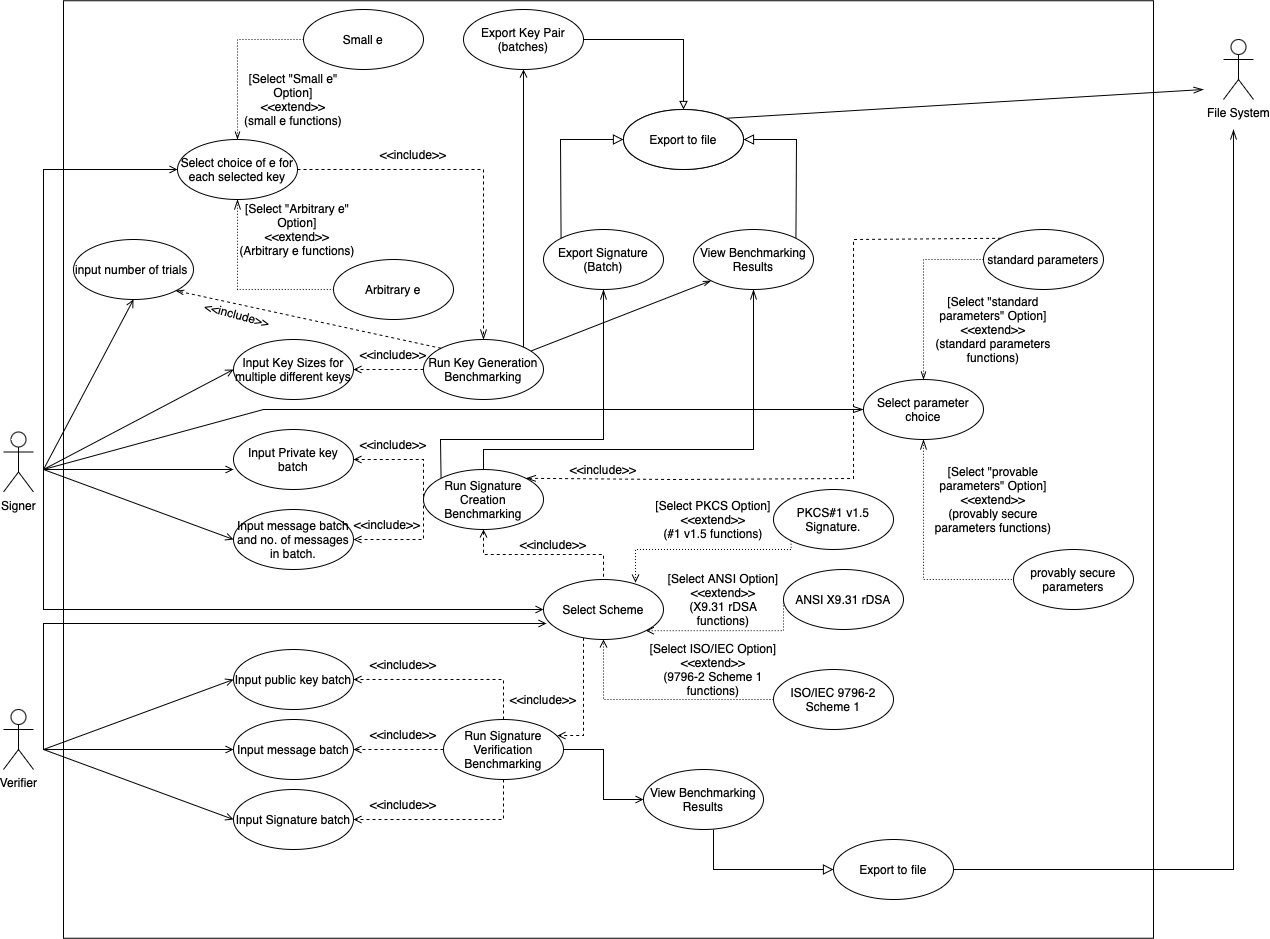
\includegraphics[scale=0.4]{main_pictures/MAIN_USE-CASE.png}
    \caption{UML Use Case Diagram}
    \label{fig:uc}
\end{figure}

Please see Appendix Appendix B.1 for a full breakdown of relevant requirements (capturing essential behaviour), and a flow-of-events type description for figure \ref{fig:uc} representing completed UML use cases, derived from preceding user stories.



\section{A Horizontal Slice: Key Generation}
\subsection{Design}
\begin{figure}[H]
    \centering
    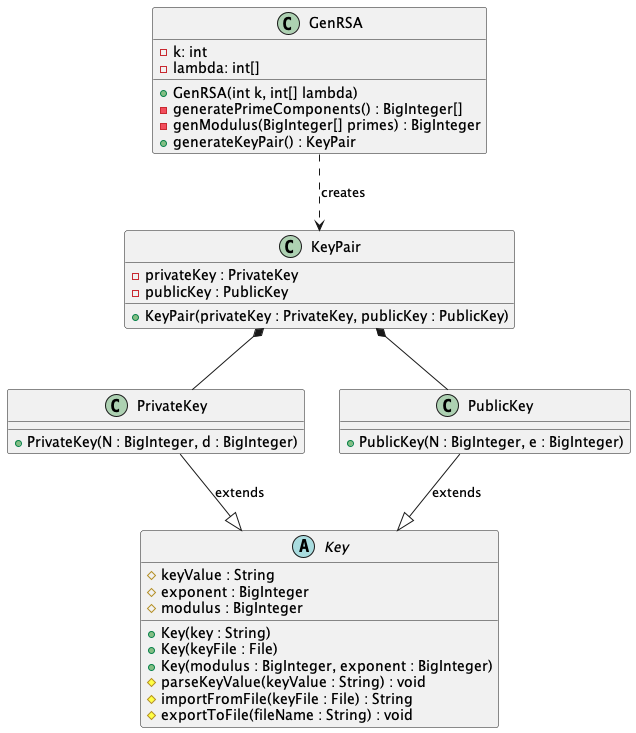
\includegraphics[scale=0.48]{main_pictures/KeyGeneration.png}
    \caption{Key Generation Class Design}
    \label{fig:kg}
\end{figure}

Figure \ref{fig:kg} provides a conceptualised design view of the foundational GenRSA definition discussed in section  \ref{subSec:keygen} with the process broken down into smaller components corresponding to roles/entities supportive to the purpose of generating keys. 


\begin{table}[H]
    \centering
    \caption{GenRSA Design}
    \label{tab:actors_description}
    \begin{tabular}{|l|p{10cm}|}
    \hline
    \textbf{Class} & \textbf{Description} \\
    \hline
    KeyGenRSA & Central class responsible for generating the key pair by providing a method to fulfil the generation process. \\
    \hline
    Key & Abstract class that serves as a blueprint for the public and private keys, encapsulating the use of the modulus and an accompanying exponent with further the ability to import/export its content. \\
    \hline
    PrivateKey / PublicKey & These classes extend from Key, specialising it for private and public key functionalities respectively. \\
    \hline
    \end{tabular}
\end{table}



\subsection{Implementation}
The approach taken to key generation deviates from standard practices by offering customisable options, particularly in the number of prime factors forming the modulus. Unlike traditional methods that limit the number of primes to two, the code allows the user to specify any number of primes, each with different bit sizes. The modulus and, consequently, the RSA key, are computed based on this specification. This approach aligns with the generalised key generation process outlined in Section \ref{subSec:keygen}. It applies as a consequence of proof implication \ref{IMP:3prime} which requires the use of a non-standard number of primes.  Specifically, the proofs require a 3-prime factor modulus configured as ($\lambda$/4, $\lambda$/4, $\lambda$/2). Under the 2v3PA[$\lambda$] (\ref{def:2v3}) this is deemed to be indistinguishable from the standard two-prime factor modulus (N = pq) thus still acting in alignment with standard RSA.


\begin{lstlisting}[caption=Initialisation of parametrisable Key Generation]
public void initialise(int k, int[] lambda) throws IllegalArgumentException {
    if (lambda.length != k) {
      throw new IllegalArgumentException("Lambda array must have k elements.");
    }

    for (int bitLength : lambda) { 
      keySize += bitLength;
    }

    this.k = k;
    this.lambda = lambda;
  }
 \end{lstlisting}
 
The suitability of Java's BigInteger class as discussed prior becomes evident from the outset. For example when the considering a foundational task: RSA Key Generation and more precisely the generation of the large primes required to encompass the modulus N.
Utilising the constructor BigInteger(int bitLength, int certainty, Random rnd), it is possible to generate probable prime numbers of some arbitrary value, providing a certainty level is indicated.
\begin{lstlisting}[caption=Parametrisable Prime Generation with BigInteger]
public BigInteger[] generatePrimeComponents() {
    BigInteger[] components = new BigInteger[k];
    for (int i = 0; i < k; i++) {
      components[i] = new BigInteger(lambda[i], this.certainty, new SecureRandom());
    }
    return components;
  }
\end{lstlisting}
This leads to the first step to be taken in any implementation of RSA: the initialisation of large prime numbers. 
Due to the magnitude of possible integers required in question, attempting to factorise both p and q to establish their primality with absolute certainty is computationally impractical. Instead, BigInteger employs the Miller-Rabin primality test to assess the probability of primality based on the probability  \[ 1 - \frac{1}{2^{certainty}}\]
For a balance between security and practicality, a certainty value between 50-100 is typical. I chose the midpoint value as a practical compromise.


\begin{lstlisting}[caption= Adaptation for specification of small e]
 private int eBitLength;
 
 public GenRSA(int k, int[] lambda, boolean isSmallE) throws IllegalArgumentException {
    initialise(k, lambda);
    eBitLength = isSmallE ? keySize / 4 : keySize;
  }
  
  public BigInteger computeE(BigInteger phi) {
    BigInteger e = new BigInteger(eBitLength, new SecureRandom());
    while (e.compareTo(ONE) <= 0 || !phi.gcd(e).equals(ONE) || e.compareTo(phi) >= 0) {
      e = new BigInteger(eBitLength, new SecureRandom());
    }
    return e;
  }
\end{lstlisting}

Another novel aspect of this implementation as per implication \ref{IMP:PHI} of the $\varphi$-Hiding Assumption, is the provision for a small public exponent \( e \leqslant N^{1/4} \). This is initiated by providing an additional constructor that includes an isSmallE flag to specify whether a small e is desired. The bit length of e is then calculated accordingly.  If a small \( e \) is chosen, its bit length is set to a quarter of the key size, ensuring compliance as per the considered proof. Otherwise, \( e \)'s bit length matches that of \( \phi \). In either case we have it that \( e \), belongs to the group \( (Z/ Z_{\phi})^{\times} \) meeting standard RSA requirements.

The remaining computation in the attempt to obtain the private exponent d is straightforward with a naturally supported modInverse operation.
\begin{lstlisting}[caption=Java Implementation of Key Generation (\ref{subSec:keygen})]
  
  public KeyPair generateKeyPair() {
    BigInteger[] primes = this.generatePrimeComponents();
    BigInteger N = genModulus(primes);
    BigInteger phi = computePhi(primes);
    BigInteger e = computeE(phi);
    
    BigInteger d = e.modInverse(phi);
    PublicKey publicKey = new PublicKey(N, e);
    PrivateKey privateKey = new PrivateKey(N, primes, phi, e, d);

    return new KeyPair(publicKey, privateKey);
  }

\end{lstlisting}


\section{Design}

\textcolor{red} {For other types of design documentation, please see Appendix B.2.}

This section depicts the structure of classes to be used in the implementation of the project deliverable. For brevity, The section details the design only up to the SignatureController Assembly. The remaining components are detailed at the beginning of Appendix B.2. It can however be noted that the application's modular structure is consistent throughout, so the design principles and patterns applied here for the signature module are similarly reflected across all other modules. 

Embedded within the architecture is a deliberate emphasis on separation of concerns, following the Model-View-Controller (MVC) design pattern. In general terms, MVC separates the application into three interconnected components: the 'Model' for the application's data, the 'View' for the user interface, and the 'Controller' for managing user inputs and updating the Model and View accordingly.
\subsection{Design of Main Controller: Orchestration of Application Flow}


\begin{figure}[H]
    \centering
    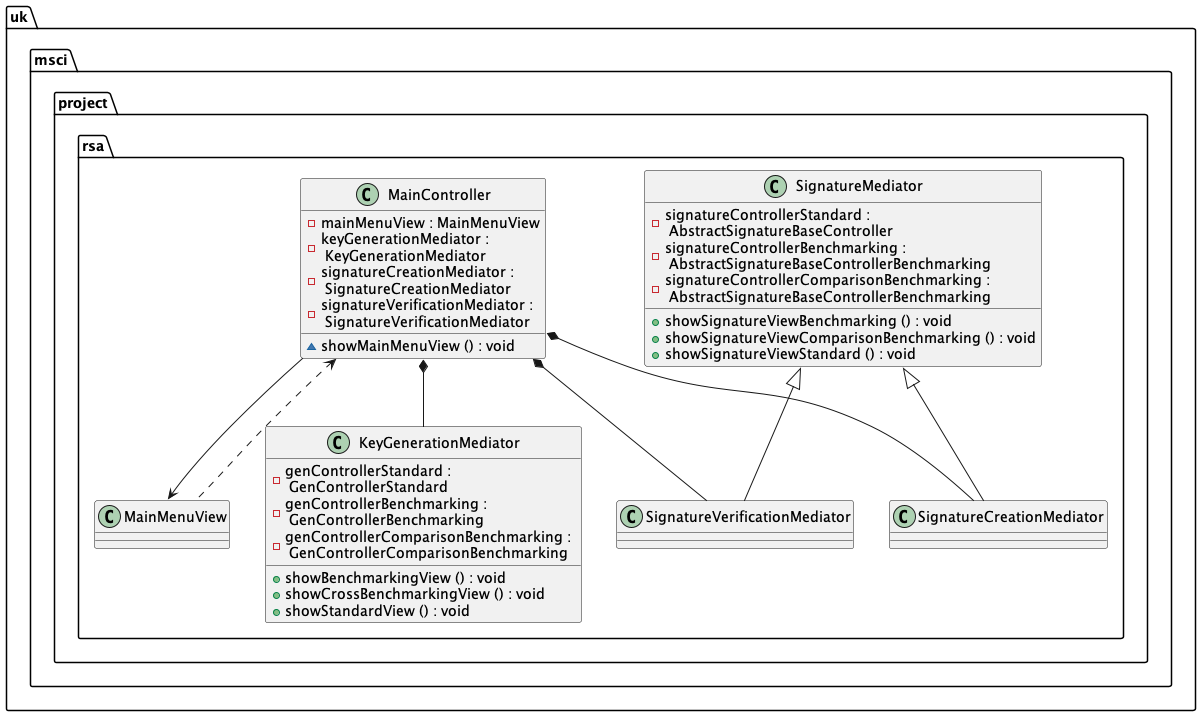
\includegraphics[width=\textwidth]{main_pictures/mainController.png}
    \caption{Design of Main Controller: Orchestration of Application Flow}
    \label{fig:MAINCONTROLLERDESIGN}
\end{figure}


\subsection{MVC pattern}
At the heart of the design is the MainController, which orchestrates the application flow by responding to user actions and coordinating the display of different views linked to the specialised modules. 

There are two applications of the MVC coordinated by the MainController i.e., the applications two functional (pre-benchmarking) modules: the signatures and additionally the Key Generation module. Most essentially, each of these module's, controller assembly's are encapsulated using a respective mediator class. The role of the mediator classes are to act as an intermediary between the main controller of the application and controller assembly of the relevant functional module. This is required because the application is to consist of various operational modes: i.e., standard, benchmarking, and comparison benchmarking. This class ensures the appropriate controllers are utilised and configured based on the operational context and mode. The mediator pattern fulfils this by obviating the need for the MainController to interact with each controller for an application module individually. The first of these to be considered SignatureMediator.



\subsection{Signature Module}

\textbf{Design of SignatureController Assembly: Orchestration of Signature Related functionalities}

\begin{figure}[H]
    \centering
    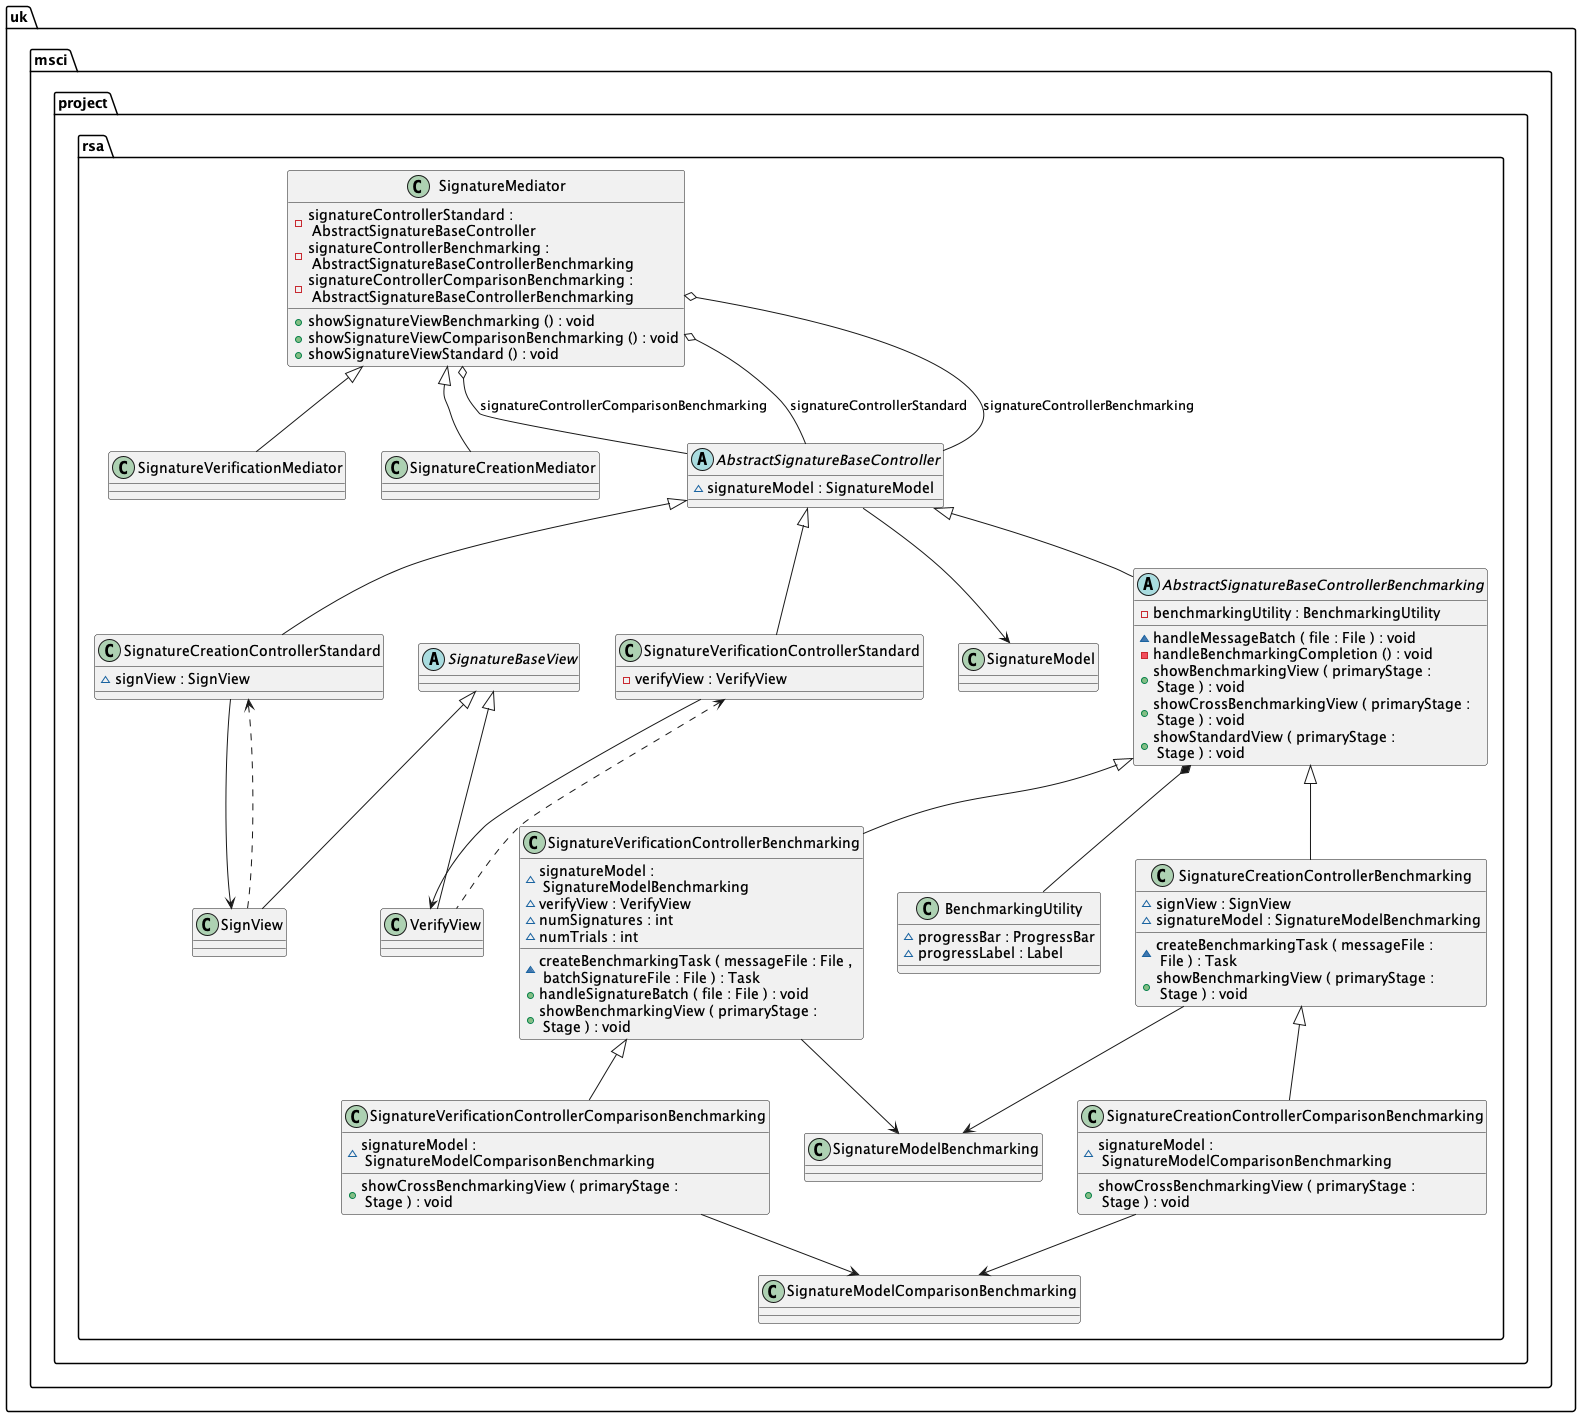
\includegraphics[width=1.2\textwidth]{main_pictures/signatureController.png}
    \caption{Design of SignatureController Assembly: Orchestration of Signature Related functionalities}
    \label{fig:SIGCONTROLLERDESIGN}
\end{figure}
Delving deeper into the orchestration of signature-related functionalities, the UML class diagram presents overview of the structure, facilitated by the SignatureMediator class.  
The SignatureMediator serves as a centralised hub acting to manage the flow between the MainController and the application mode specific signature controllers. Its design encompasses concretely the subclasses: SignatureCreationMediator and the SignatureVerificationMediator, each tasked with a specific aspect of signature processing.

The SignatureCreationMediator class is responsible for the initiation and management of signature generation. It interacts with the SignatureCreationControllerStandard (which handles single use non-benchmarked signature creation processes), and with the SignatureCreationControllerBenchmarking for recording and documenting the performance of signature schemes instantiated using differing parameter types on a batch of messages. 
The SignatureVerificationMediator mirrors this structure for the verification processes. 
\begin{comment}
It acts in concert with the SignatureVerificationControllerStandard for singular signature-message pairings and liaises with the SignatureVerificationControllerBenchmarking to handle the benchmarking of verification processes. For example, aiming to record and document the performance of signature schemes instantiated for verifying a provided message-signature batch pairing using differing parameter types.
\end{comment}
Both the SignatureCreationControllerBenchmarking and the SignatureVerificationControllerBenchmarking classes are equipped with a BenchmarkingUtility, which includes a ProgressBar component. This provides live feedback during benchmarking processes, enhancing the user experience by delivering a visual indication of the operation's progress from 0 to 100.

The subclass SignatureCreationControllerComparisonBenchmarking and its verification counterpart, SignatureVerificationControllerComparisonBenchmarking, extend normal benchmarking functionality to accommodate comparison benchmarking. They allow for the side-by-side evaluation of parameter types for a provided signature scheme by key size, offering insights into the relative performance of each signature scheme.

The SignatureModel and SignatureModelBenchmarking classes (see Appendix B.2) serve as a software approximation of a real-world processes of the signing and verification processes. They maintain the state of signature data and respectively handle standard or benchmarking mode operations thus fulfilling the processing of signatures and execution of benchmarking tasks if applicable.

The KeyGenerationMediator mirrors the structure of the SignatureMediator but is focused on generating cryptographic keys through the key generation model assembly which manages the GenRSA facilitated key creation.

\textbf{Observer pattern}

The UML diagram also hints at the observer pattern, a subset of MVC, with the Signature Controllers acting as observers to their relevant Views, which are the observables. When a user interacts with a signature view, such as initiating a signature generation request, the View notifies the SignatureController, which in turn invokes the necessary methods in both the View and the Model to fulfil the request. This decouples the user interface from the business logic, allowing for independent development and refinement of each component.


\section{Implementation: An Extensible Signature Scheme framework}
Having explored the theoretical underpinnings and practical applications of digital signature schemes, we now transition to a more technical focus of how signature schemes can be concretely implemented with a generalised framework.

The foundation of this is provided by SigSchemeInterface, an interface that outlines the essential functionalities required for any digital signature scheme. This interface serves as a contract for implementing classes, ensuring that fundamental operations such as signing, verifying, and data conversion between different formats are standardised and consistent.

\begin{lstlisting}[caption=SigSchemeInterface Interface code] 
public interface SigSchemeInterface {

  byte[] sign(byte[] M) throws SignatureException, DataFormatException;

  boolean verify(byte[] data, byte[] signature) throws SignatureException, DataFormatException;

  BigInteger OS2IP(byte[] EM);

  byte[] I2OSP(BigInteger m) throws IllegalArgumentException;

  BigInteger RSASP1(BigInteger m);

  BigInteger RSAVP1(BigInteger s);
}
 \end{lstlisting}

Signing a message m (sign(m)) works as follows:
\begin{enumerate}
\item Encode the message: encodeMessage(m).

\item Convert the message to representative integer form: OS2IP(m).

\item Using a private key sk, calculate the signature representative s using RSA: RSASP1(sk, m).

\item Convert the signature (integer) representative back to a byte string: I2OSP(s).
\end{enumerate}

Verification is the reverse, adapted accordingly. Given a signature s (verify(s)):

\begin{enumerate}
\item Convert s into an integer representative: OS2IP(s).

\item Using public key vk, calculate the message representative m: RSAVP1(vk, s)

\item Convert m to a byte string: I2OSP(m).

\item Verify the byte string using verifyMessage.
\end{enumerate}

This generalised flow presents two further methods: 'encodeMessage', an algorithm to format data before performing a cryptographic signing operation on its integer representation, and 'verifyMessage', an algorithm that verifies the signature after a cryptographic verification operation has been performed on its integer representation. 
 
Building upon the SigSchemeInterface, the abstract class SigScheme is introduced as a concrete implementation of the Interface for implementing RSA-based signature schemes. This class provides standardised implementations of the interface's methods and 
includes additional functionality specific to RSA operations. It encapsulates key components like the RSA modulus, exponent, and message digest, contributing to a modular and extensible design suitable for various RSA-based signature schemes.

\begin{lstlisting}[caption=Implementation of RSA primitives]

  /**
   * Converts a BigInteger to an octet string of length emLen is the byte length of the RSA modulus.
   */
  public byte[] I2OSP(BigInteger m) throws IllegalArgumentException {
    return ByteArrayConverter.toFixedLengthByteArray(m, this.emLen);
  }

  /**
   * Calculates the RSA signature of a given message representative by raising it to the power of
   * the private exponent as outlined by the RSA algorithm.
   */
  public BigInteger RSASP1(BigInteger m) {
    BigInteger s = m.modPow(this.exponent, this.modulus);
    return s;
  }

  /**
   * Facilitates the verification of RSA signature by raising it to the power of the public exponent
   * as outlined by the RSA algorithm.
   */
  public BigInteger RSAVP1(BigInteger s) {
    return this.RSASP1(s);
  }

}
 \end{lstlisting}
We note that the implementation of RSAVP1 re-uses RSASP1. This design choice is viable because the exponent field in the SigScheme class is generic and can represent either the public or private exponent, depending on the type of key the scheme is instantiated with. This reuse simplifies the code and centralises the modular exponentiation logic in one place.
\newline

\begin{lstlisting}[caption=]
  public BigInteger OS2IP(byte[] EM) {
    return new BigInteger(1, EM);
  }
 \end{lstlisting}
For octet string to integer conversion, the BigInteger(int signum, byte[] magnitude) constructor provides a concise application of the concept succinctly converting the byte array that represents an octet string. The signum is set to 1 (since messages are non-negative) and the byte array of the message acts as the magnitude. The end result is a BigInteger representation of the message, which can then be used in RSA signing or verification processes.

 

\begin{lstlisting}[caption=Signature Scheme specialisation methods]
  // Abstract method to be implemented by derived classes for encoding
  protected abstract byte[] encodeMessage(byte[] M) throws DataFormatException;

  public boolean verifyMessage(byte[] M, byte[] S)
      throws DataFormatException {
    BigInteger s = OS2IP(S);
    BigInteger m = RSAVP1(s);
    byte[] EM;
    try {
      EM = I2OSP(m);
    } catch (IllegalArgumentException e) {
      return false;
    }

    byte[] EMprime = encodeMessage(M);

    return Arrays.equals(EM, EMprime);
  }
 \end{lstlisting}
 
The SigScheme class provides two further methods as compared to the interface with encodeMessage and verifyMessage. The encodeMessage method is left abstract because the encoding of messages is essentially what distinguishes different signature schemes. On the other hand, verifyMessage has a standardised implementation because, in many cases, it simply reverses the signing process. Since the core logic of this reversal often follows a standard procedure that is largely independent of the specifics of the message encoding, it is feasible to provide a standardised implementation for verifyMessage within the SigScheme class.

\subsection*{Message Recovery}

Message recovery schemes, such as ISO/IEC 9796-2 Scheme 1, represent a special case, thereby challenging the notion of standardised implementations for key methods like sign and verifyMessage.
\begin{lstlisting}[caption=Implementation changes for Message Recovery Schemes]
public abstract class SigScheme implements SigSchemeInterface {

  byte[] nonRecoverableM;

  byte[] recoverableM;
}
public class ISO_IEC_9796_2_SCHEME_1 extends SigScheme {
  @Override
  public byte[] sign(byte[] M) throws DataFormatException {
    byte[] S = super.sign(M);
    // Extract m2 from the original message M using the computed m2's length
    if (m2Len > 0) {
      nonRecoverableM = Arrays.copyOfRange(M, m1Len - m2Len, m1Len);
    }
    return S;
  }
}
 \end{lstlisting}
The sign method for these schemes needs to be able to set the non recoverable message field of the class, to allow the respective portion message to be returned to the user, as part of the conclusion to the signature creation process. Hence, the ISO/IEC 9796-2 Scheme 1 class includes an overridden implementation of sign modified accordingly to account for this.

Along these same lines the verifyMessage method which we omit for brevity has to incorporate logic related to the separation of the message into recoverable/non-recoverable parts into the verification process. During verification, the verifyMessage method must correctly reconstruct the original message from these two parts. 

\section{Implementation: Enabling a Provably Secure hash output}
\label{hashOutput} 

This implementation includes support for an unusually large hash output (\(|H()| \ge \frac{\lambda}{2}\)) as required by both proofs. This is accomplished using variable length hash functions like SHAKE-128, or via MGF1 applied to fixed-length functions such as SHA-256.


 \begin{lstlisting}[caption=Retrieval of Message Digest Instances]
public class DigestFactory {
  public static MessageDigest getMessageDigest(DigestType digestType)
      throws NoSuchAlgorithmException, NoSuchProviderException {
    switch (digestType) {
      case SHA_256 -> {return MessageDigest.getInstance("SHA-256");}
      case MGF_1_SHA_256 -> {return MessageDigest.getInstance("SHA-256");}
      case SHA_512 -> {return MessageDigest.getInstance("SHA-512");}
      case MGF_1_SHA_512 -> {return MessageDigest.getInstance("SHA-512");}
      case SHAKE_128 -> {Security.addProvider(new BouncyCastleProvider());
        return MessageDigest.getInstance("SHAKE128", BouncyCastleProvider.PROVIDER_NAME);
      }
      case SHAKE_256 -> {Security.addProvider(new BouncyCastleProvider());
      return MessageDigest.getInstance("SHAKE256", BouncyCastleProvider.PROVIDER_NAME);}
      default -> throw new NoSuchAlgorithmException("Unsupported digest type: " + digestType);
    }
  }
}
 \end{lstlisting}
An enumeration (enum) `DigestType` classifies each hash function. To abstract their creation, a factory pattern is used, which provides a consistent interface to obtain `MessageDigest` objects for each signature scheme. Notably, for SHA-3 family hashes like SHAKE-128 and SHAKE-256, BouncyCastle cryptographic API is used due to the absence of native Java support.

\begin{lstlisting}[caption=Adaptation of Signature Scheme initialisation for specification of provably secure hash output ]
public abstract class SigScheme implements SigSchemeInterface {

  boolean isProvablySecureParams;
  int hashSize;
  
  public SigScheme(Key key, boolean isProvablySecureParams) {
    initialise(key);
    this.isProvablySecureParams = isProvablySecureParams;
  }
  
}
 \end{lstlisting}
To facilitate scheme instantiation with a larger hash output, constructors include an 'isProvablySecureParams' flag. This flag aids in specifying whether an enhanced security hash output is required, allowing the bit length of the hash size to be computed accordingly.



   \begin{lstlisting}[caption=Configuration of Hash Size]
public void setDigest(DigestType digestType, int customHashSize)
      throws NoSuchAlgorithmException, InvalidDigestException, NoSuchProviderException {
    md.reset();
    this.currentHashType = digestType;
    this.md = DigestFactory.getMessageDigest(digestType);
    this.hashID = getHashID(currentHashType);

    if (digestType == DigestType.SHA_256 || digestType == DigestType.SHA_512) {
      this.hashSize = md.getDigestLength(); // Fixed size
    } else if (isProvablySecureParams) {
      this.hashSize = (emLen + 1) / 2; // Provably secure size
    } else {
      if (customHashSize <= 0) {
        throw new IllegalArgumentException("Custom hash size must be a positive integer");
      }
      this.hashSize = customHashSize; // Custom size for variable-length hash types
    }
  }
 \end{lstlisting}

The setDigest method configures the hash size based on the hash type and operational parameters. For fixed size hashes (e.g., SHA-256, SHA-512), it sets the size corresponding to the digest type. For variable-length hashes (e.g., SHAKE-128, SHAKE-256), it offers two options: a preset provably secure size (half the length of the modulus) or a user-defined custom size.


\begin{comment}
This option for a custom size provides extra flexibility since in theory, a provably secure hash output size is not limited to being  half the length of the modulus, and in fact any custom  \textit{Hash output $\displaystyle|H()| \ge \displaystyle\frac{\lambda}{2}$} fulfils the criteria for being provably secure respective to a corresponding key. Additionally it allows for generalised usage of the variable length hash functions within the considered signature schemes thereby facilitating other unrelated use cases and adhering to the principle of scalable design.
\end{comment}

After the hash function is determined and the hash output size configured, marking the final step of the hashing process, the computation of the actual hash within the signature scheme is required.
  \begin{lstlisting}[caption=Final Computation of hash]
public byte[] computeHashWithOptionalMasking(byte[] message) {
    if (!(currentHashType == DigestType.SHA_256 || currentHashType == DigestType.SHA_512)) {
      if (currentHashType == DigestType.MGF_1_SHA_256
          || currentHashType == DigestType.MGF_1_SHA_512) {
        return new MGF1(this.md).generateMask(message, this.hashSize);
      } else {
        return computeShakeHash(message);
      }
    } else {
      return computeHash(message);
    }
  }
 \end{lstlisting}
Finally, the computeHashWithOptionalMasking method calculates the hash within the signature scheme. It handles variable length hash functions distinctively, especially for MGF1, which requires generating a mask using the determined hash size.




\section{Implementation: Application Overview}
The application comprises four main portals, each linked to functionalities essential for facilitating digital signatures. These portals allow transition between standard and benchmarking-specific operations.
\begin{enumerate}
    \item \textbf{Main Menu:} The gateway to key and signature functionalities within the application.
    \item \textbf{Key Generation:} Allows generation of RSA key pairs, either singularly for standard operations or in batches for benchmarking purposes.
    \item \textbf{Signature Creation:} Facilitates creation of individual signatures in standard mode or signature batches in benchmarking mode for deterministic signature types.
    \item \textbf{Signature Verification:} Enables validation of individual or batch signatures against messages or message batches, respectively, in standard or benchmarking modes.
\end{enumerate}


\textbf{Focus on Comparison Benchmarking:}

\begin{comment}
 including Benchmarking (default), Comparison Benchmarking, and Custom Comparison Benchmarking. However this 
\end{comment}
The application offers four modalities, categorised into standard mode and a suite of benchmarking modes. This section focusses on the preset Comparison Benchmarking mode since it most directly aligns with the project's aim to assess the burden on computational time that arises when using provably secure parameters in deterministic RSA signature schemes. Please see the user manual for a user friendly explanation of the remaining modes.


Comparison Benchmarking mode offers a direct comparative analysis between standard and provably secure key configuration groups (with user selected hash functions for each group). This allows evaluation of the performance of the Standard and Provably Secure groupings, with all trials repeated for every hash function and key configuration combination for each group. Results are then presented side by side in a table and/or overlaid graphs for each entered key size.

\subsection{Main Menu}

\begin{figure}[H]
    \centering
    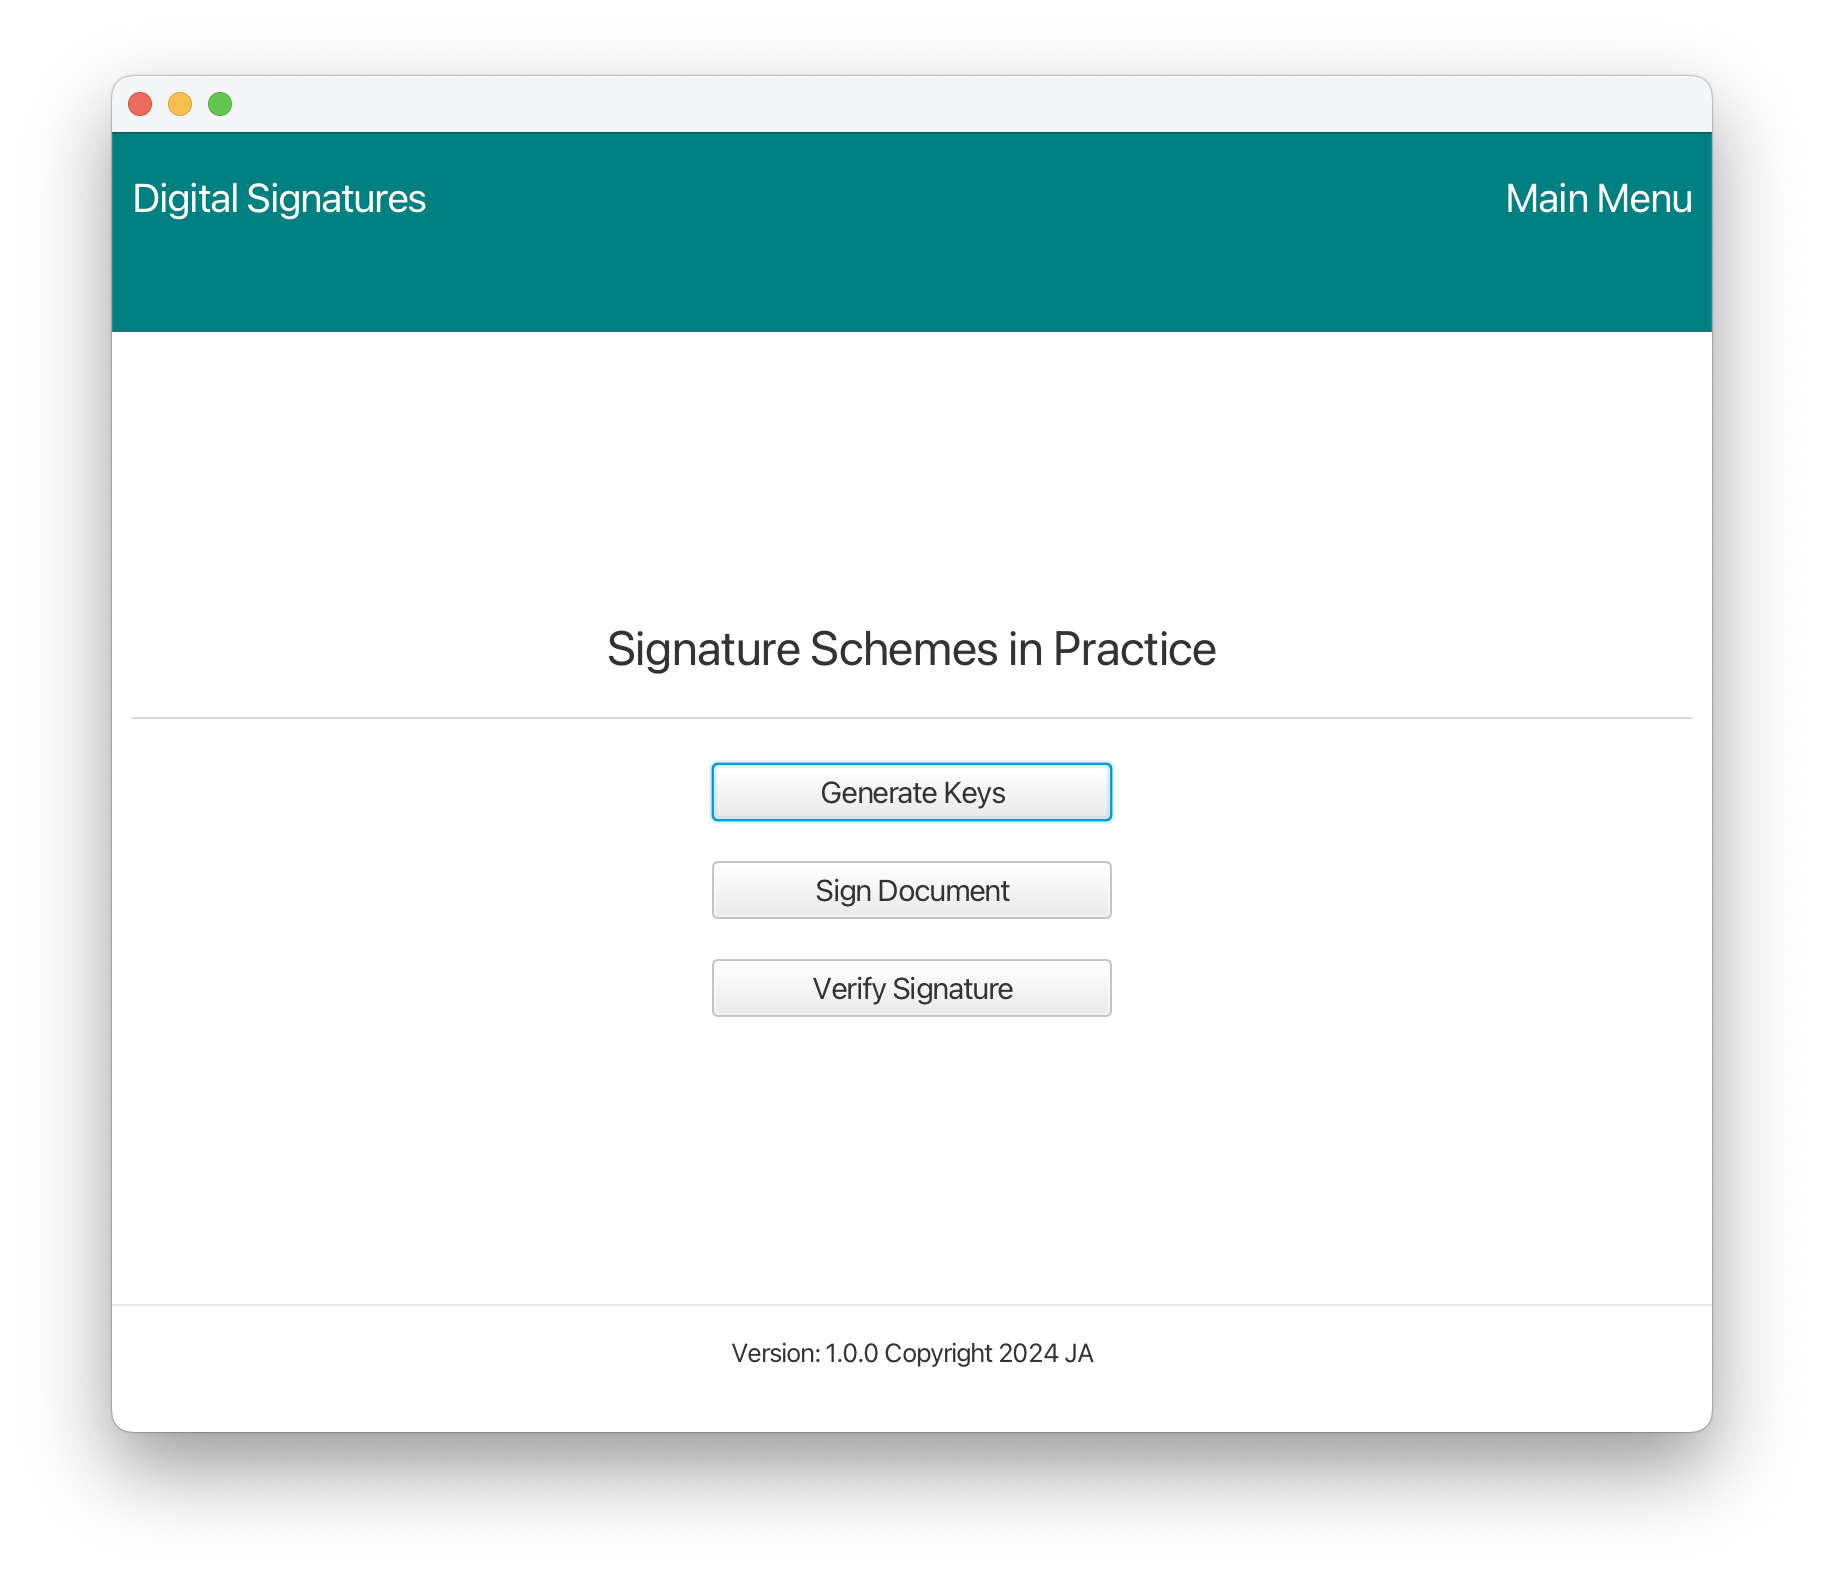
\includegraphics[scale=0.4]{main_pictures/ui/mainMenu.png}
    \caption{Main Menu}
\end{figure}
The main menu screen of the application presents a straightforward and functional layout, serving as the gateway to its core features via menu buttons. Its design is realised through an FXML layout file, which defines the graphical user interface elements such as buttons. Each button on the main menu is associated with a specific functionality and is observable by the virtue of its MainMenu domain object class. On launch, the MainController registers observers on the observable components of the main menu screen. User interactions prompt the corresponding observer to trigger its effects. The equivalent pattern is followed for all other components in the design of the program. From this point we assume its usage.

\begin{comment}
 For example, the "Generate Keys" button is linked to the following method contained in the class:
\begin{lstlisting}[caption=Mechanism for registering observers]
@FXML private Button generateKeysButton;

void addGenerateKeysObserver(EventHandler<ActionEvent> observer) {
  generateKeysButton.setOnAction(observer);
}
\end{lstlisting}
This mechanism enables the MainController to register observers and observe the main menu, while also underpinning the main menu by setting the primary stage of the application and displaying the MainMenuView as the initial scene.


\begin{lstlisting}[caption=MainController registering an observer to be notified on selection of key generation button]
void showMainMenuView() {
  FXMLLoader loader = new FXMLLoader(getClass().getResource("/MainMenuView.fxml"));
  Parent root = loader.load();
  mainMenuView = loader.getController();
  primaryStage.setScene(new Scene(root));
  primaryStage.show();

  mainMenuView.addGenerateKeysObserver(new GenerateKeysButtonObserver());
  // ...additional observers for other buttons
}
\end{lstlisting}
On launch, the MainController registers observers on the observable components of the main menu screen. User interactions prompt the corresponding observer to trigger its effects.  For example  clicking the "Generate Keys" button, will the trigger GenerateKeysButtonObserver to display of the key generation interface through the KeyGenerationMediator. The mediator serves as an intermediary to the key generation controller assembly. It activates the relevant controller i.e., GenControllerBenchmarking in this case, which in turn presents the user with the appropriate key generation interface in alignment with the system's default state.

\begin{lstlisting}[caption=Implementation of an observer]
public class MainController {
  class GenerateKeysButtonObserver implements EventHandler<ActionEvent> {
    @Override
    public void handle(ActionEvent event) {
      keyGenerationMediator.showBenchmarkingView();
    }
  }
  }
\end{lstlisting}
The equivalent pattern is followed for all other components in the design of the program. From this point we assume its usage.

\end{comment}
\subsection{Key Generation}
\begin{figure}[H]
    \centering % Center the images
    
    % First image in a minipage
    \begin{minipage}{0.495\textwidth}
        \centering
        \fbox{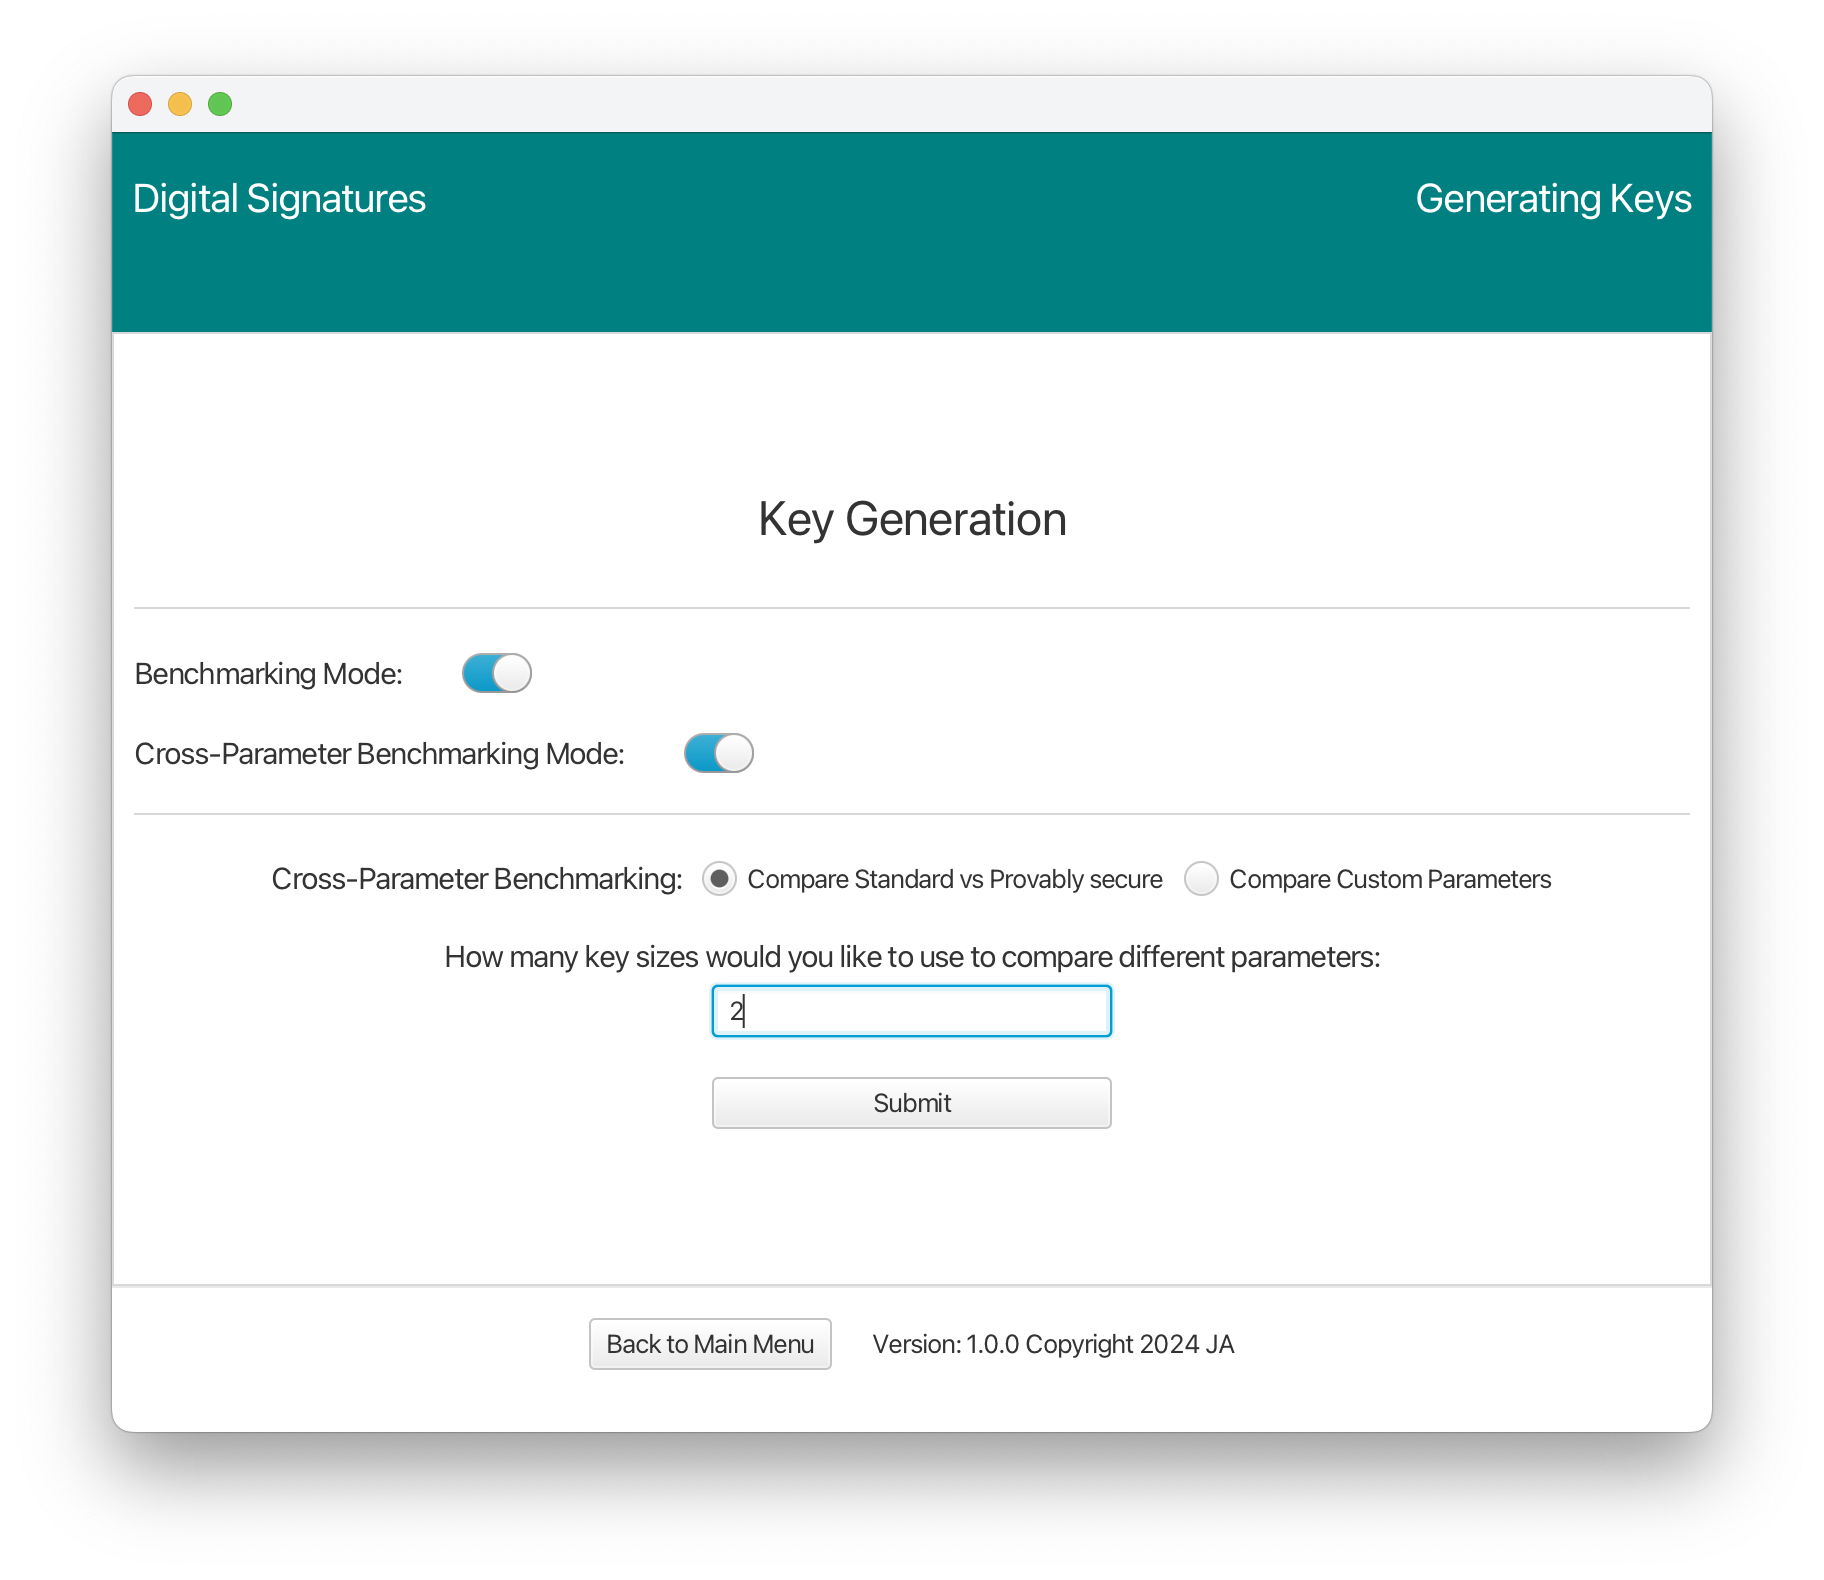
\includegraphics[width=\textwidth]{main_pictures/ui/keyGen/keyGen1.png}} % Adding border here
        \caption{Comparison Benchmarking: Key Generation (number of key sizes)}
        \label{fig:image1}
    \end{minipage}
    \hfill % Add some space between the images
    % Second image in a minipage
    \begin{minipage}{0.495\textwidth}
        \centering
        \fbox{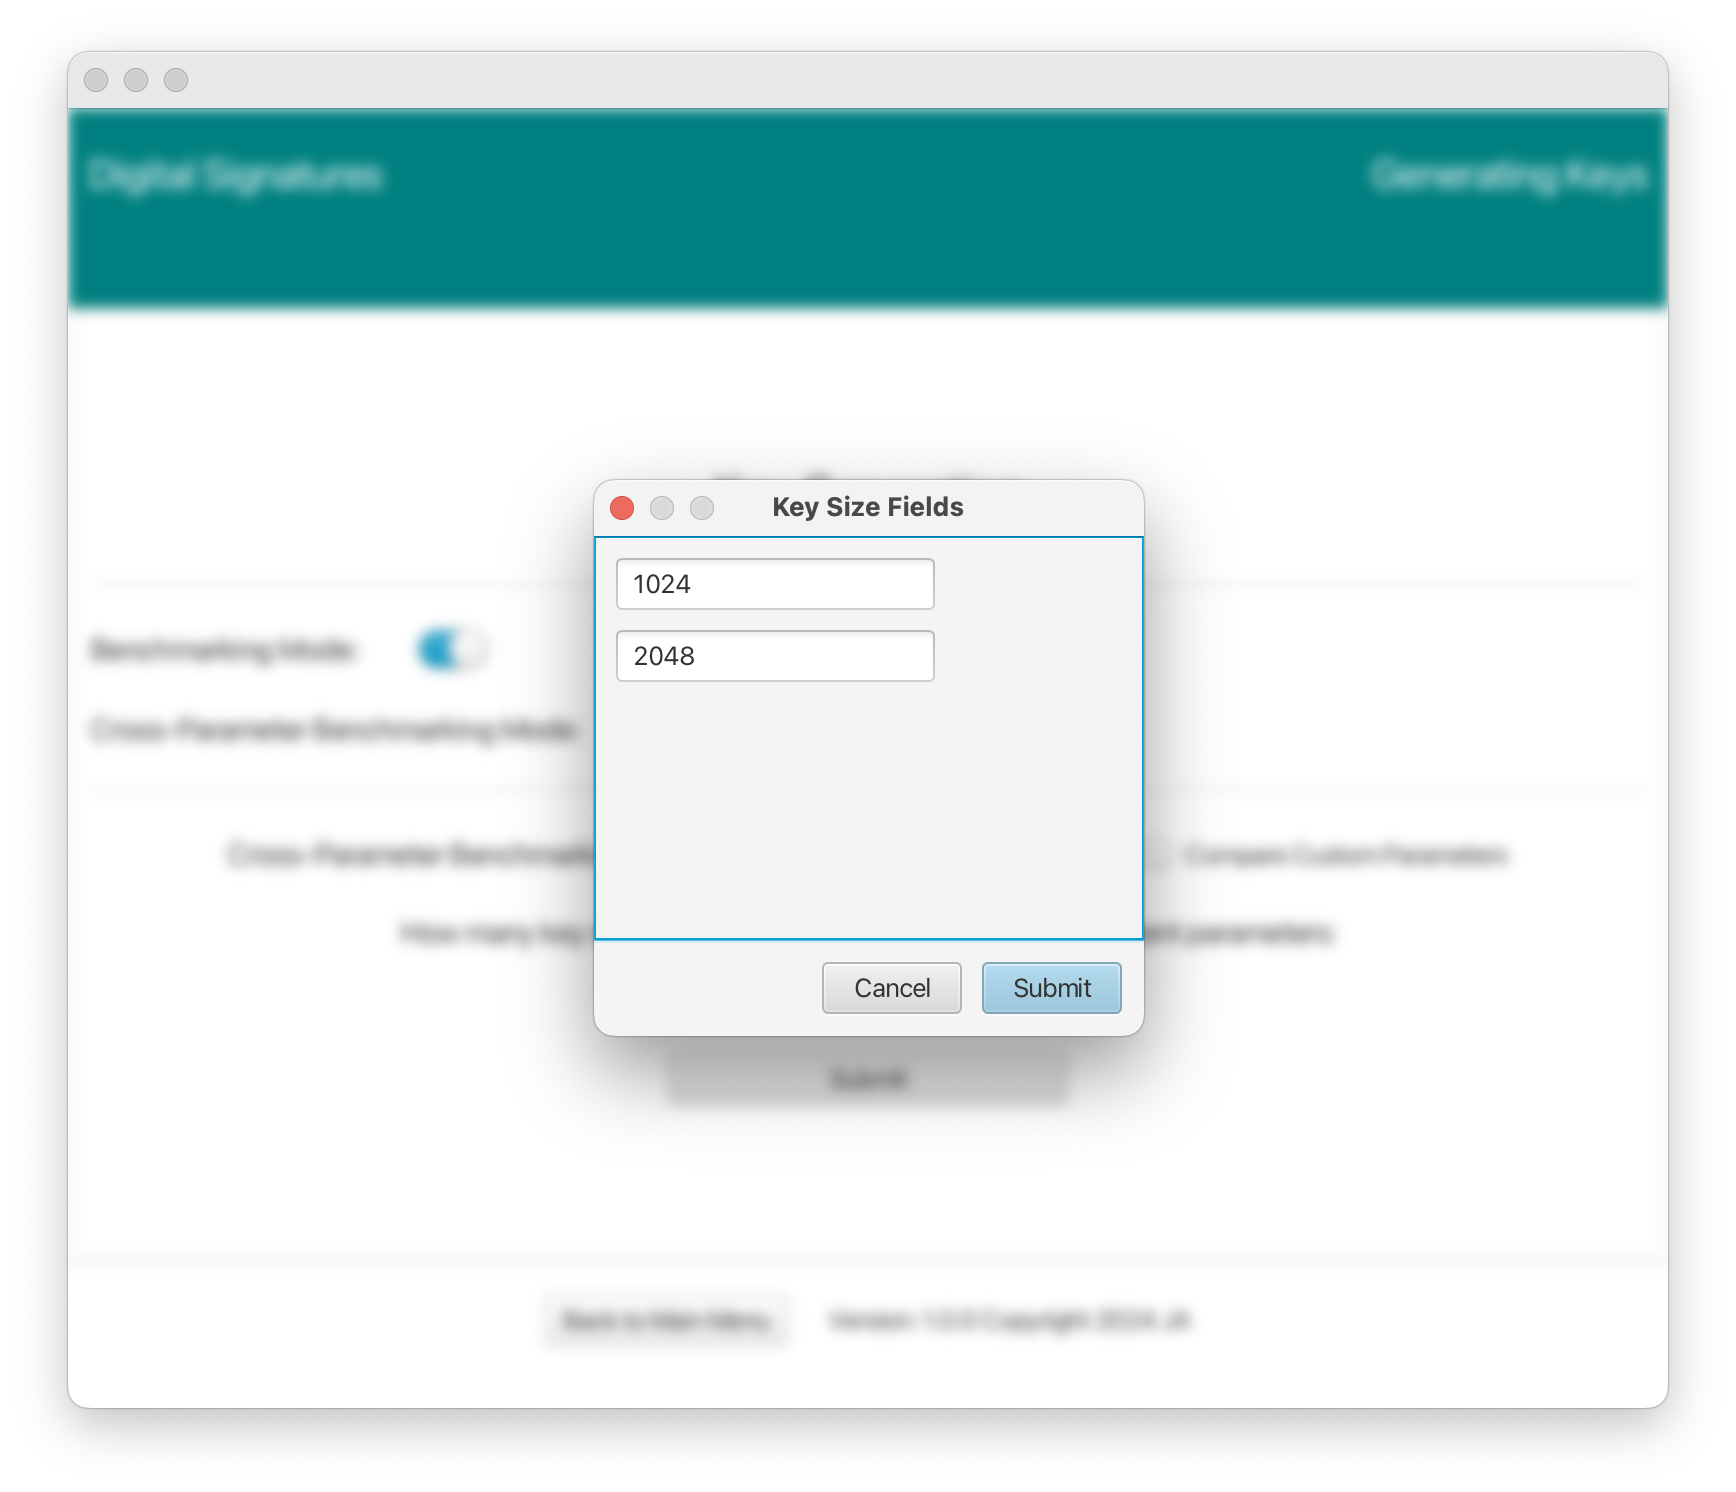
\includegraphics[width=\textwidth]{main_pictures/ui/keyGen/keyGen2.png}} % Adding border here
        \caption{Comparison Benchmarking: Key Generation (key sizes)}
        \label{fig:image2}
    \end{minipage}
    
     \begin{minipage}{0.55\textwidth}
        \centering
        \fbox{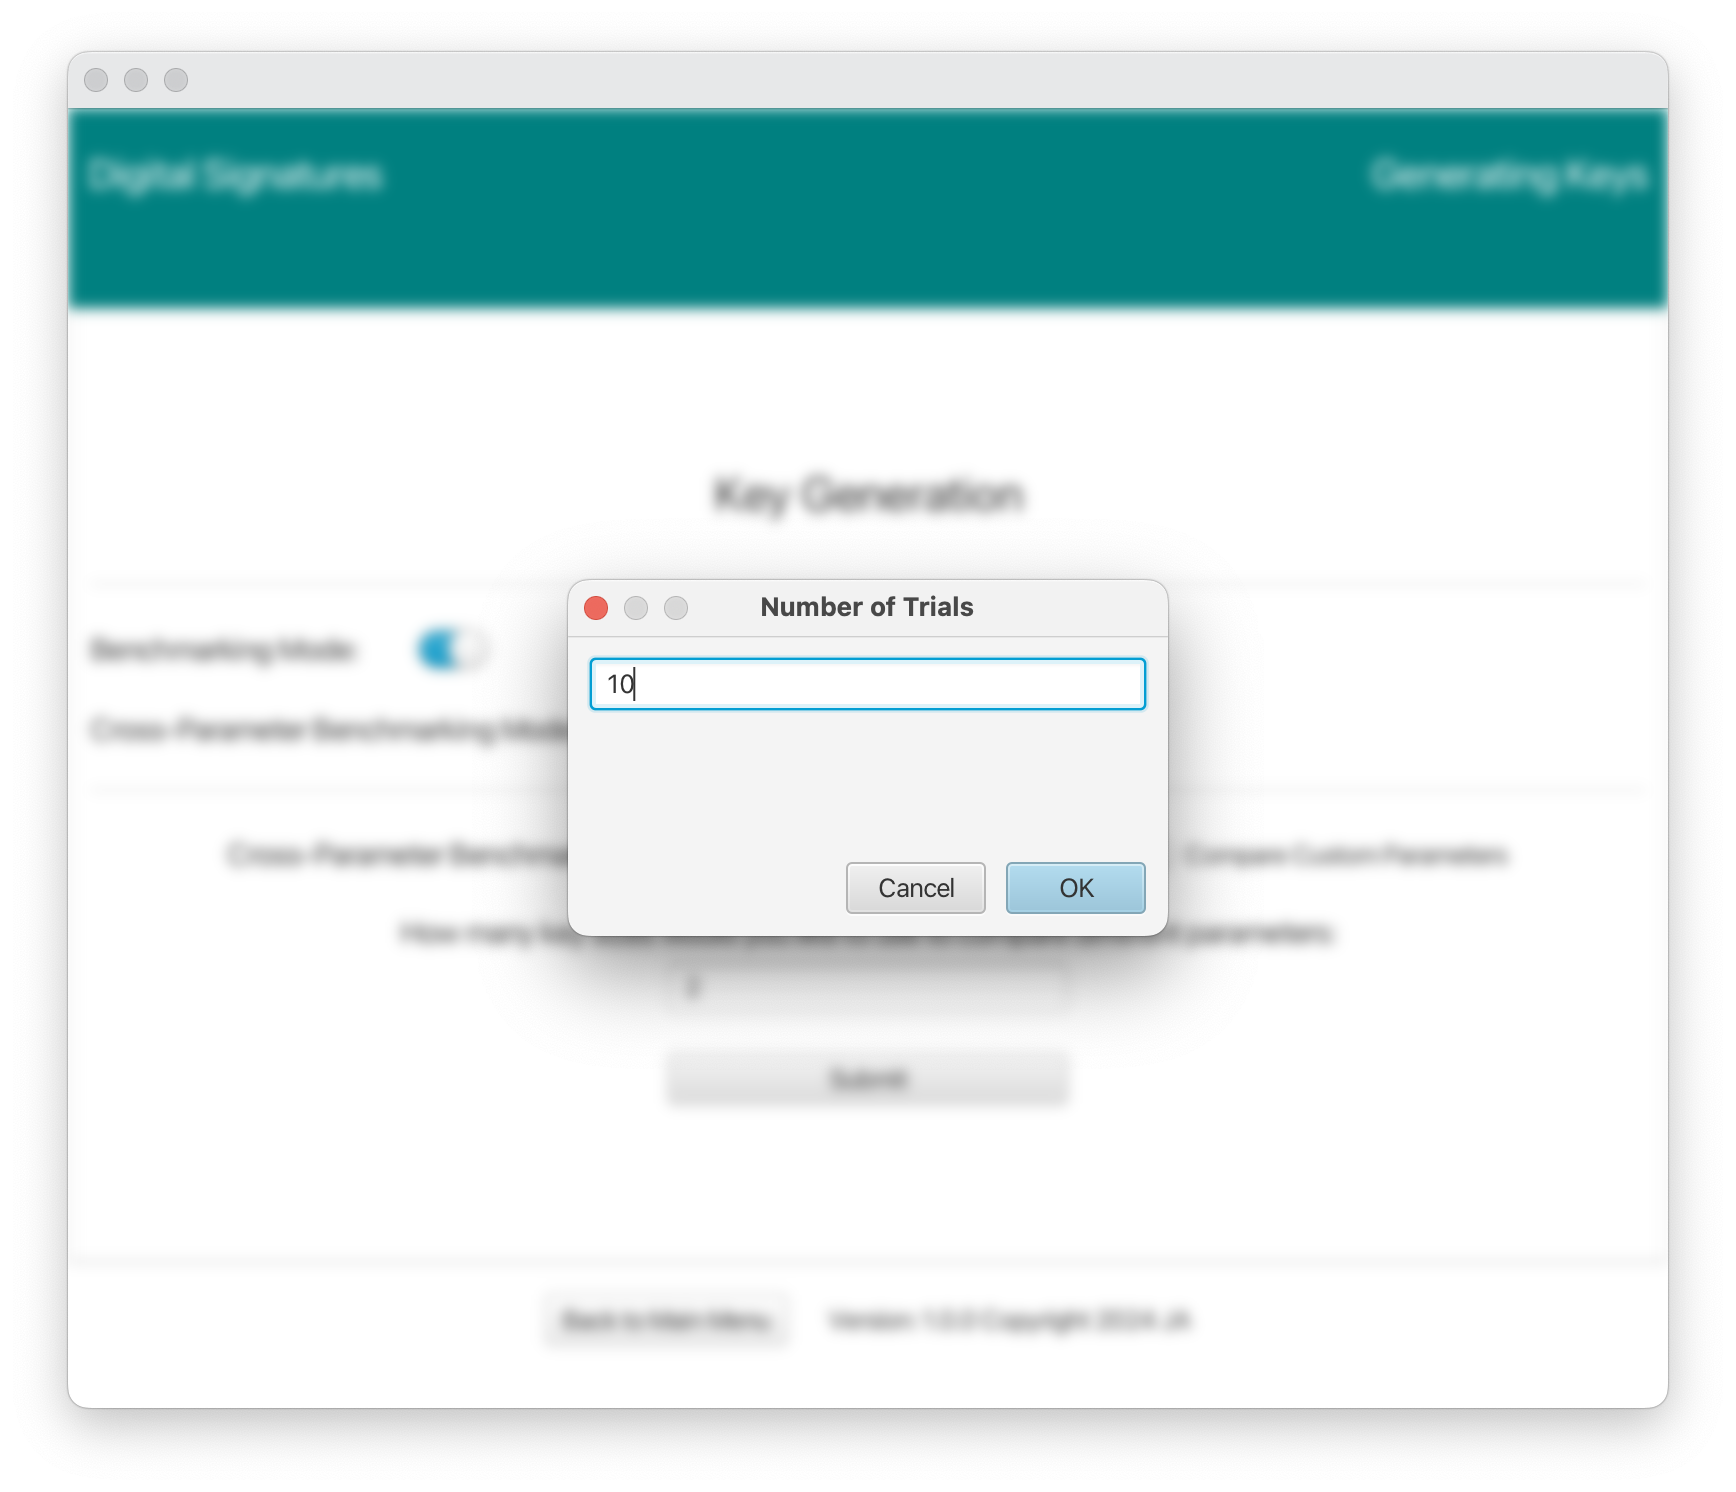
\includegraphics[width=\textwidth]{main_pictures/ui/keyGen/keyGen3.png}} % Adding border here
        \caption{Comparison Benchmarking: Key Generation (number of trials)}
        \label{fig:image2}
    \end{minipage}
\end{figure}
The key generation interface for comparison benchmarking is activated through a toggle switch. This interface offers a radio button to select the default comparison benchmarking mode, which compares standard and provably secure key configurations. Users specify the number of key sizes they wish to test, and corresponding input fields are displayed for each size (e.g., Key Size 1: 1024, Key Size 2: 2048).

For each entered key size, the application generates two groups of key configurations:
\begin{itemize}
    \item A \textbf{Standard Parameters} group, with both 2-prime and 3-prime modulus configurations and arbitrary e values.
    \item A \textbf{Provably Secure Parameters} group, with 2-prime and 3-prime modulus configurations and small e values.
\end{itemize}

Users then input the desired number of trials for key generation benchmarking, such as 10 trials. The application executes these trials for each of the four key configurations at the selected key sizes.

\begin{comment}
The GenController class manages the process flow, validating inputs for format and range. Upon confirming the number of trials, the GenModel initiates the benchmarking, with a progress bar indicating real-time completion status.

The initial key generation screen for cross-parameter (comparison) benchmarking is activated by switching on its relevant toggle switch. The first option featured by the screen is a radio button selection for the mode of comparison benchmarking to activate, on  clicking of the submit button. It is the default comparison mode option which facilitates comparison of preset key configuration groupings corresponding to standard and provably secure parameters. After inputting a number corresponding to a desired number of key sizes e.g., 2, a dynamic dialog is displayed with a matching number of key size fields to input individual key sizes e.g., Key Size 1: 1024, Key Size 2: 2048.

This triggers the application on initiation of benchmarking to do the following, for each of the entered key sizes:
\begin{itemize}
\item generate one group of key configurations for \textbf{standard parameters} inclusive of the key configurations for the 2 and 3 prime factor modulus settings i.e., Key 1: $\lambda$/4, $\lambda$/4, $\lambda$/2 \textbf{with arbitrary e} and Key 2: $\lambda$/2, $\lambda$/2 \textbf{with arbitrary e}.
\item generate a second group of key configurations for \textbf{provably secure parameters} inclusive of the key configurations for the 2 and 3 prime factor modulus settings i.e., Key 3: $\lambda$/4, $\lambda$/4, $\lambda$/2 \textbf{with small e} and Key 4: $\lambda$/2, $\lambda$/2 \textbf{with small e}.
\end{itemize}

Subsequently via an updated dialog, the number of  trials intended for the benchmarking of the key generation process can then be entered. In the current scenario with 10 trials, a benchmarking run would consist of running 10 key generations for each of the 4 key configurations for the selected key sizes.

Behind the scenes, the GenController class orchestrates flow between these various stages. Inputs submitted for any stage are subjected to a validation process. This ensures that the provided bit sizes are in an acceptable format and within the operational range for key generation or that more generally submitted inputs are positive integers.
Clicking the "OK" button on the number of trials dialog sets the benchmarking process in motion and engages the GenModel to perform the task. A progress bar is displayed for a length of time spanning the duration of the task allowing for real-time indication of progress.
\end{comment}

\begin{figure}[H]
    \centering
    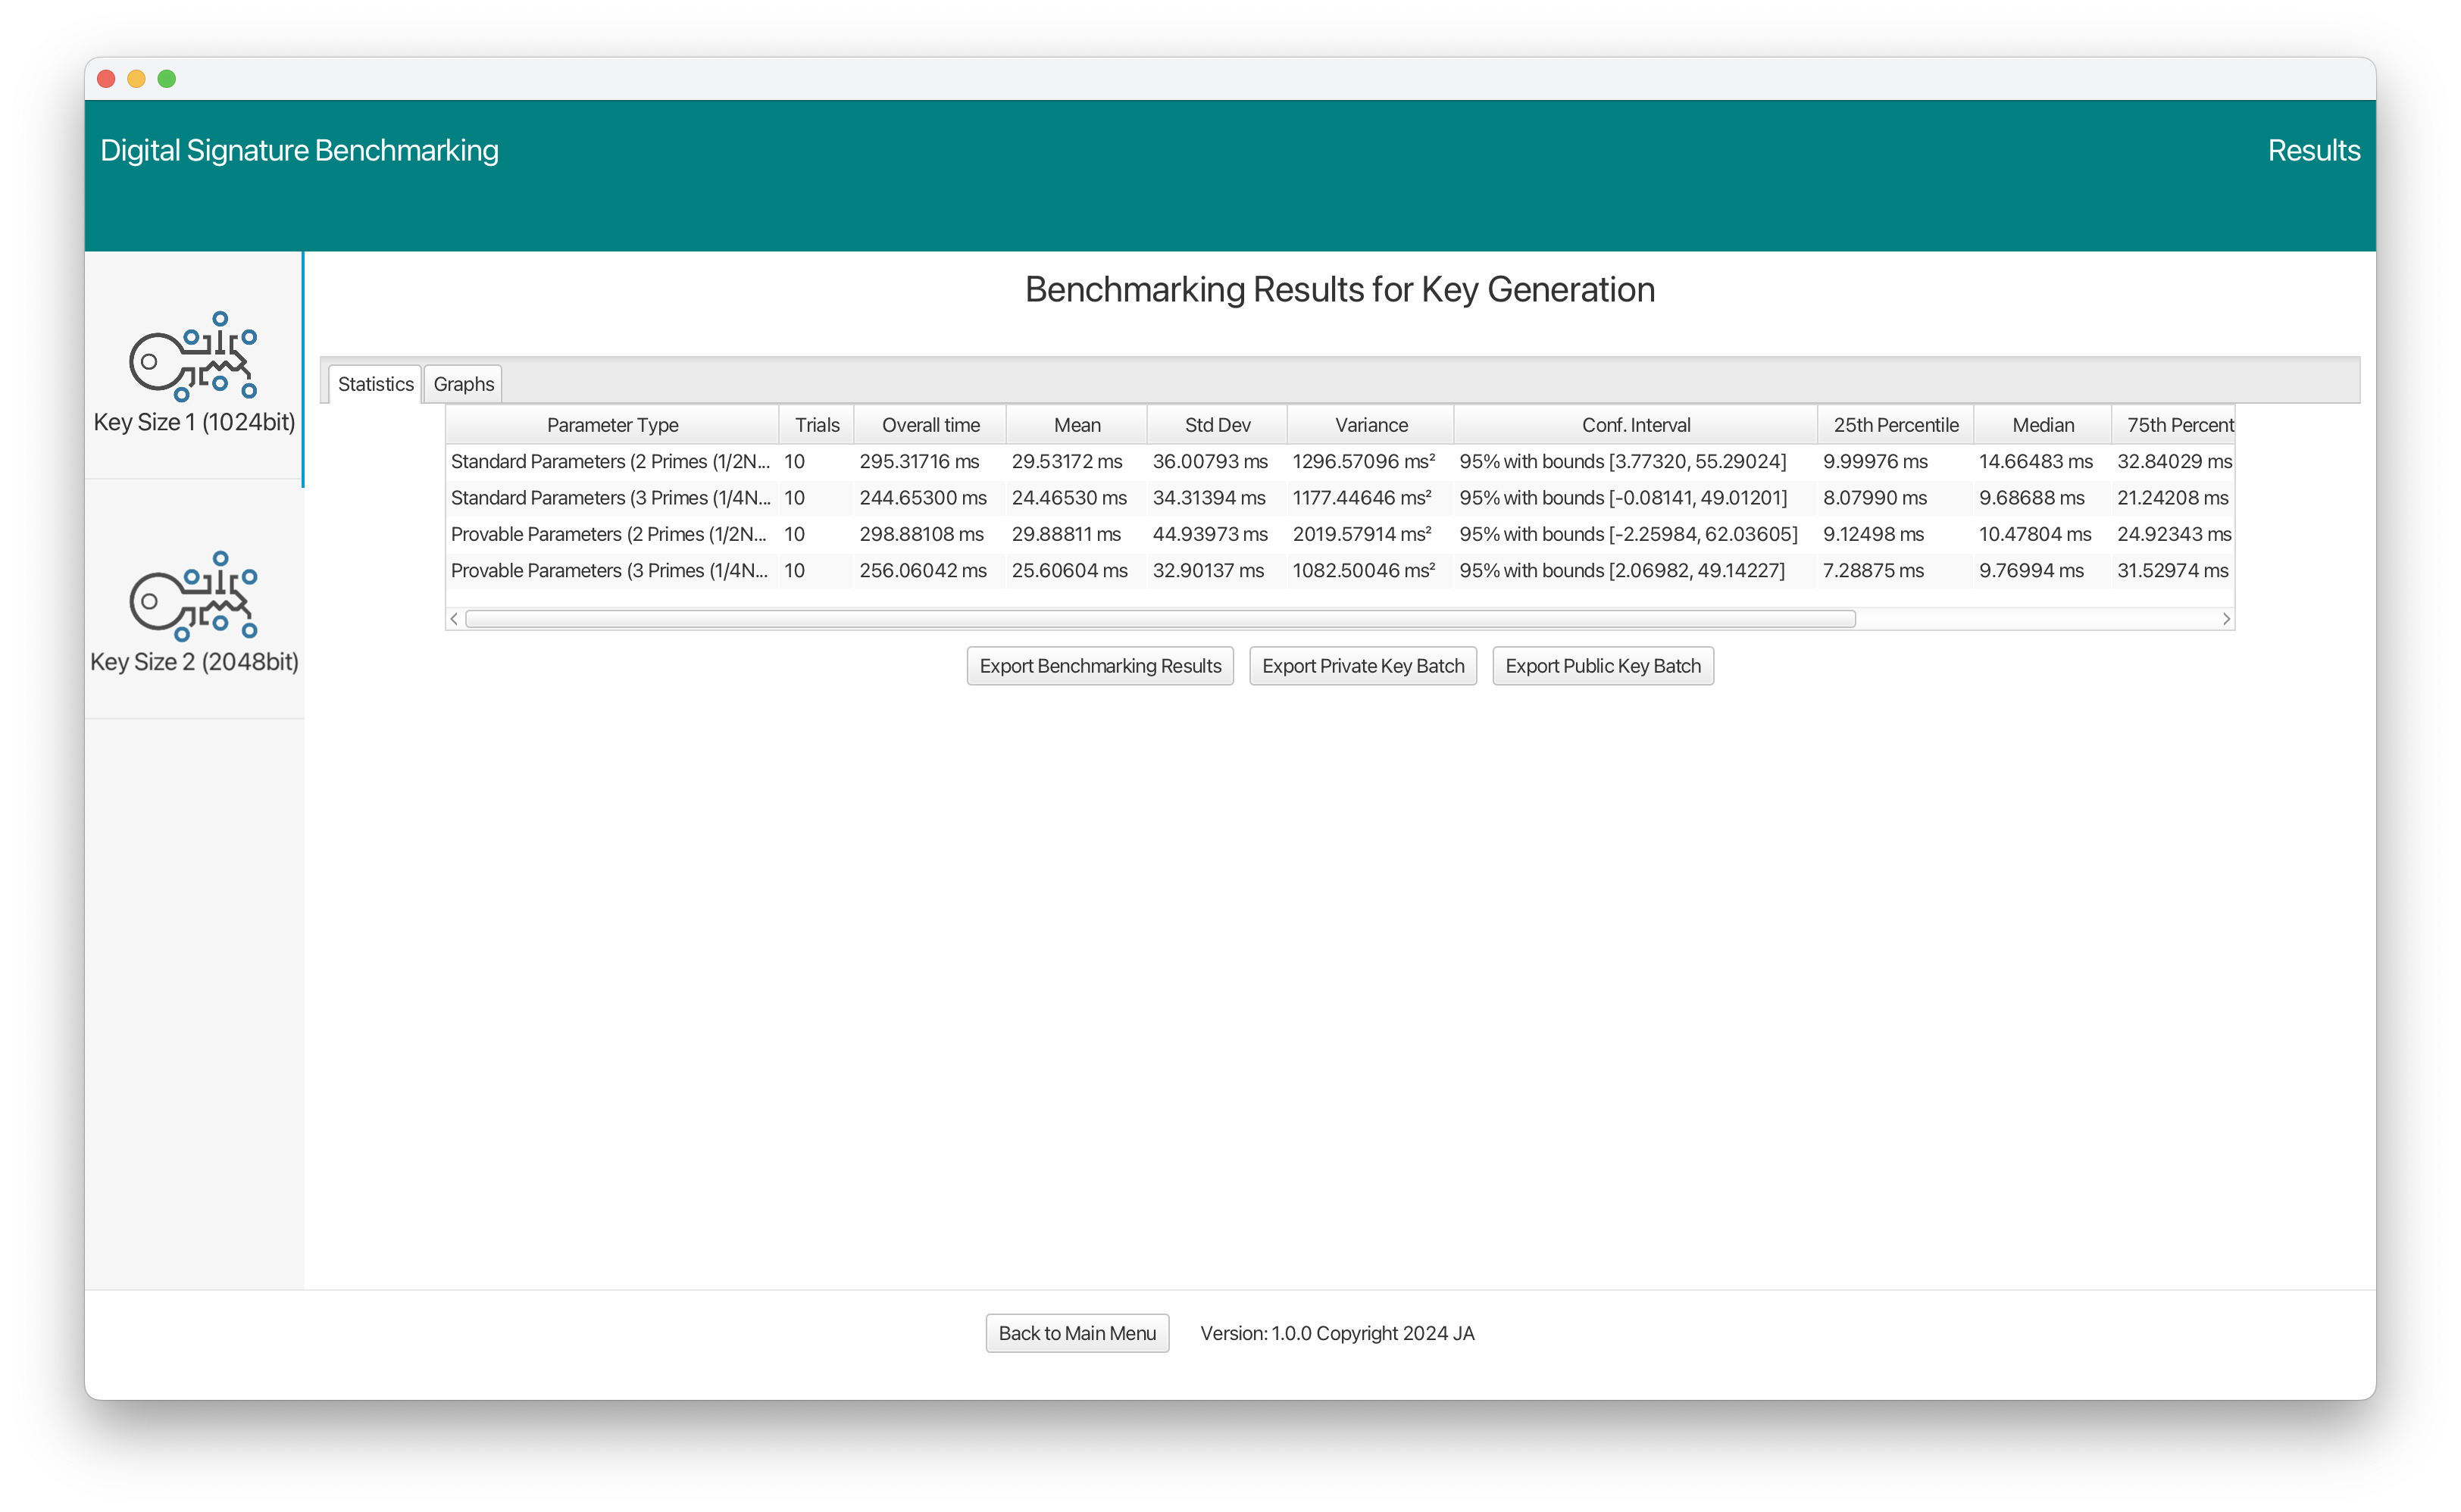
\includegraphics[scale= 0.325]{main_pictures/ui/keyGen/keyGen4.png}
    \caption{Comparison Benchmarking: Key Generation (Results Screen)}
\end{figure}
Upon completion of benchmarking, the ResultsController is engaged to display the results from benchmarking. The results screen contains a side pane with buttons corresponding to each individual key size previously entered. Within each side tab, the results table displays a row by row sequence of statistical metrics for all 4 key configurations.  The ordering is by parameter set (i.e., 2 key configurations for standard parameter key results first, followed by the 2 key configurations for provably secure parameter results second). Below the results table, the application also provides the functionality to export the benchmarking results and if desired public or private key batches corresponding to a global set of keys matching the key configurations enumerated in a sequence for all key sizes.




\begin{figure}[H]
    \centering % Center the images
    
    % First image in a minipage
    \begin{minipage}{0.7\textwidth}
        \centering
        \fbox{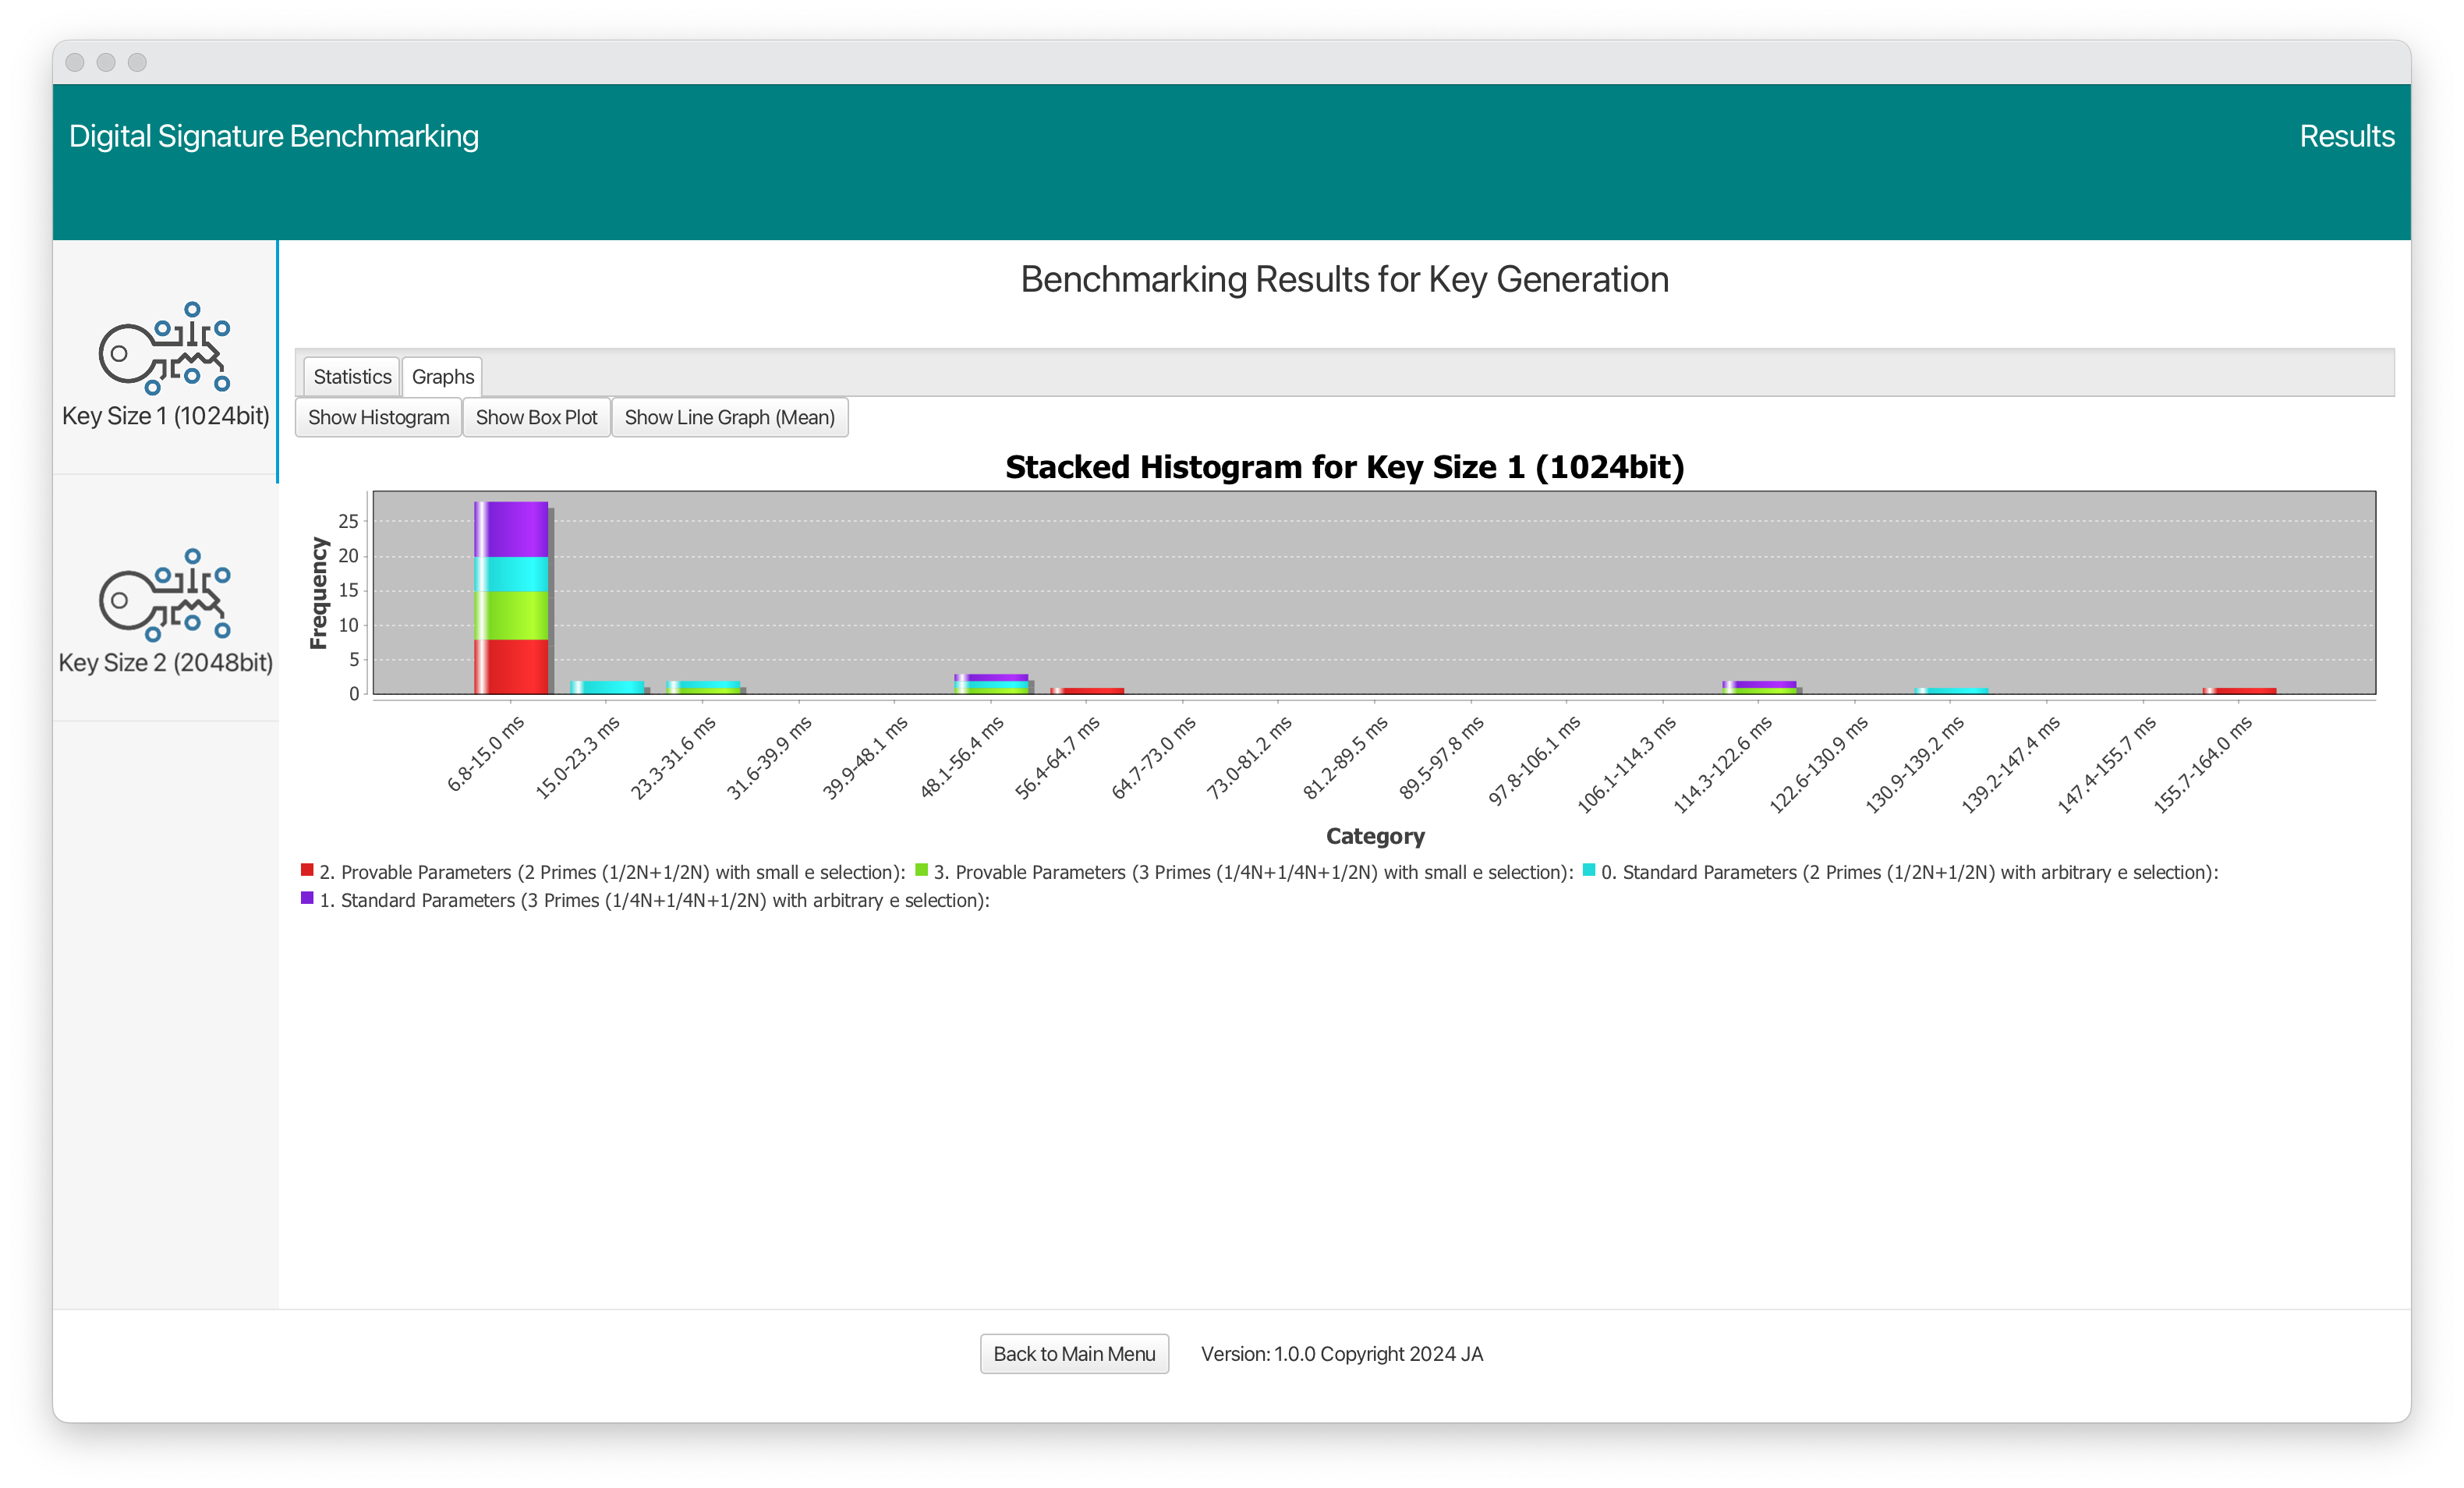
\includegraphics[width=\textwidth]{main_pictures/ui/keyGen/keyGen5.png}} % Adding border here
        \caption{Comparison Benchmarking: Key Generation: Overlaid Histogram}
        \label{fig:image1}
    \end{minipage}
    \hfill % Add some space between the images
    % Second image in a minipage
    \begin{minipage}{0.7\textwidth}
        \centering
        \fbox{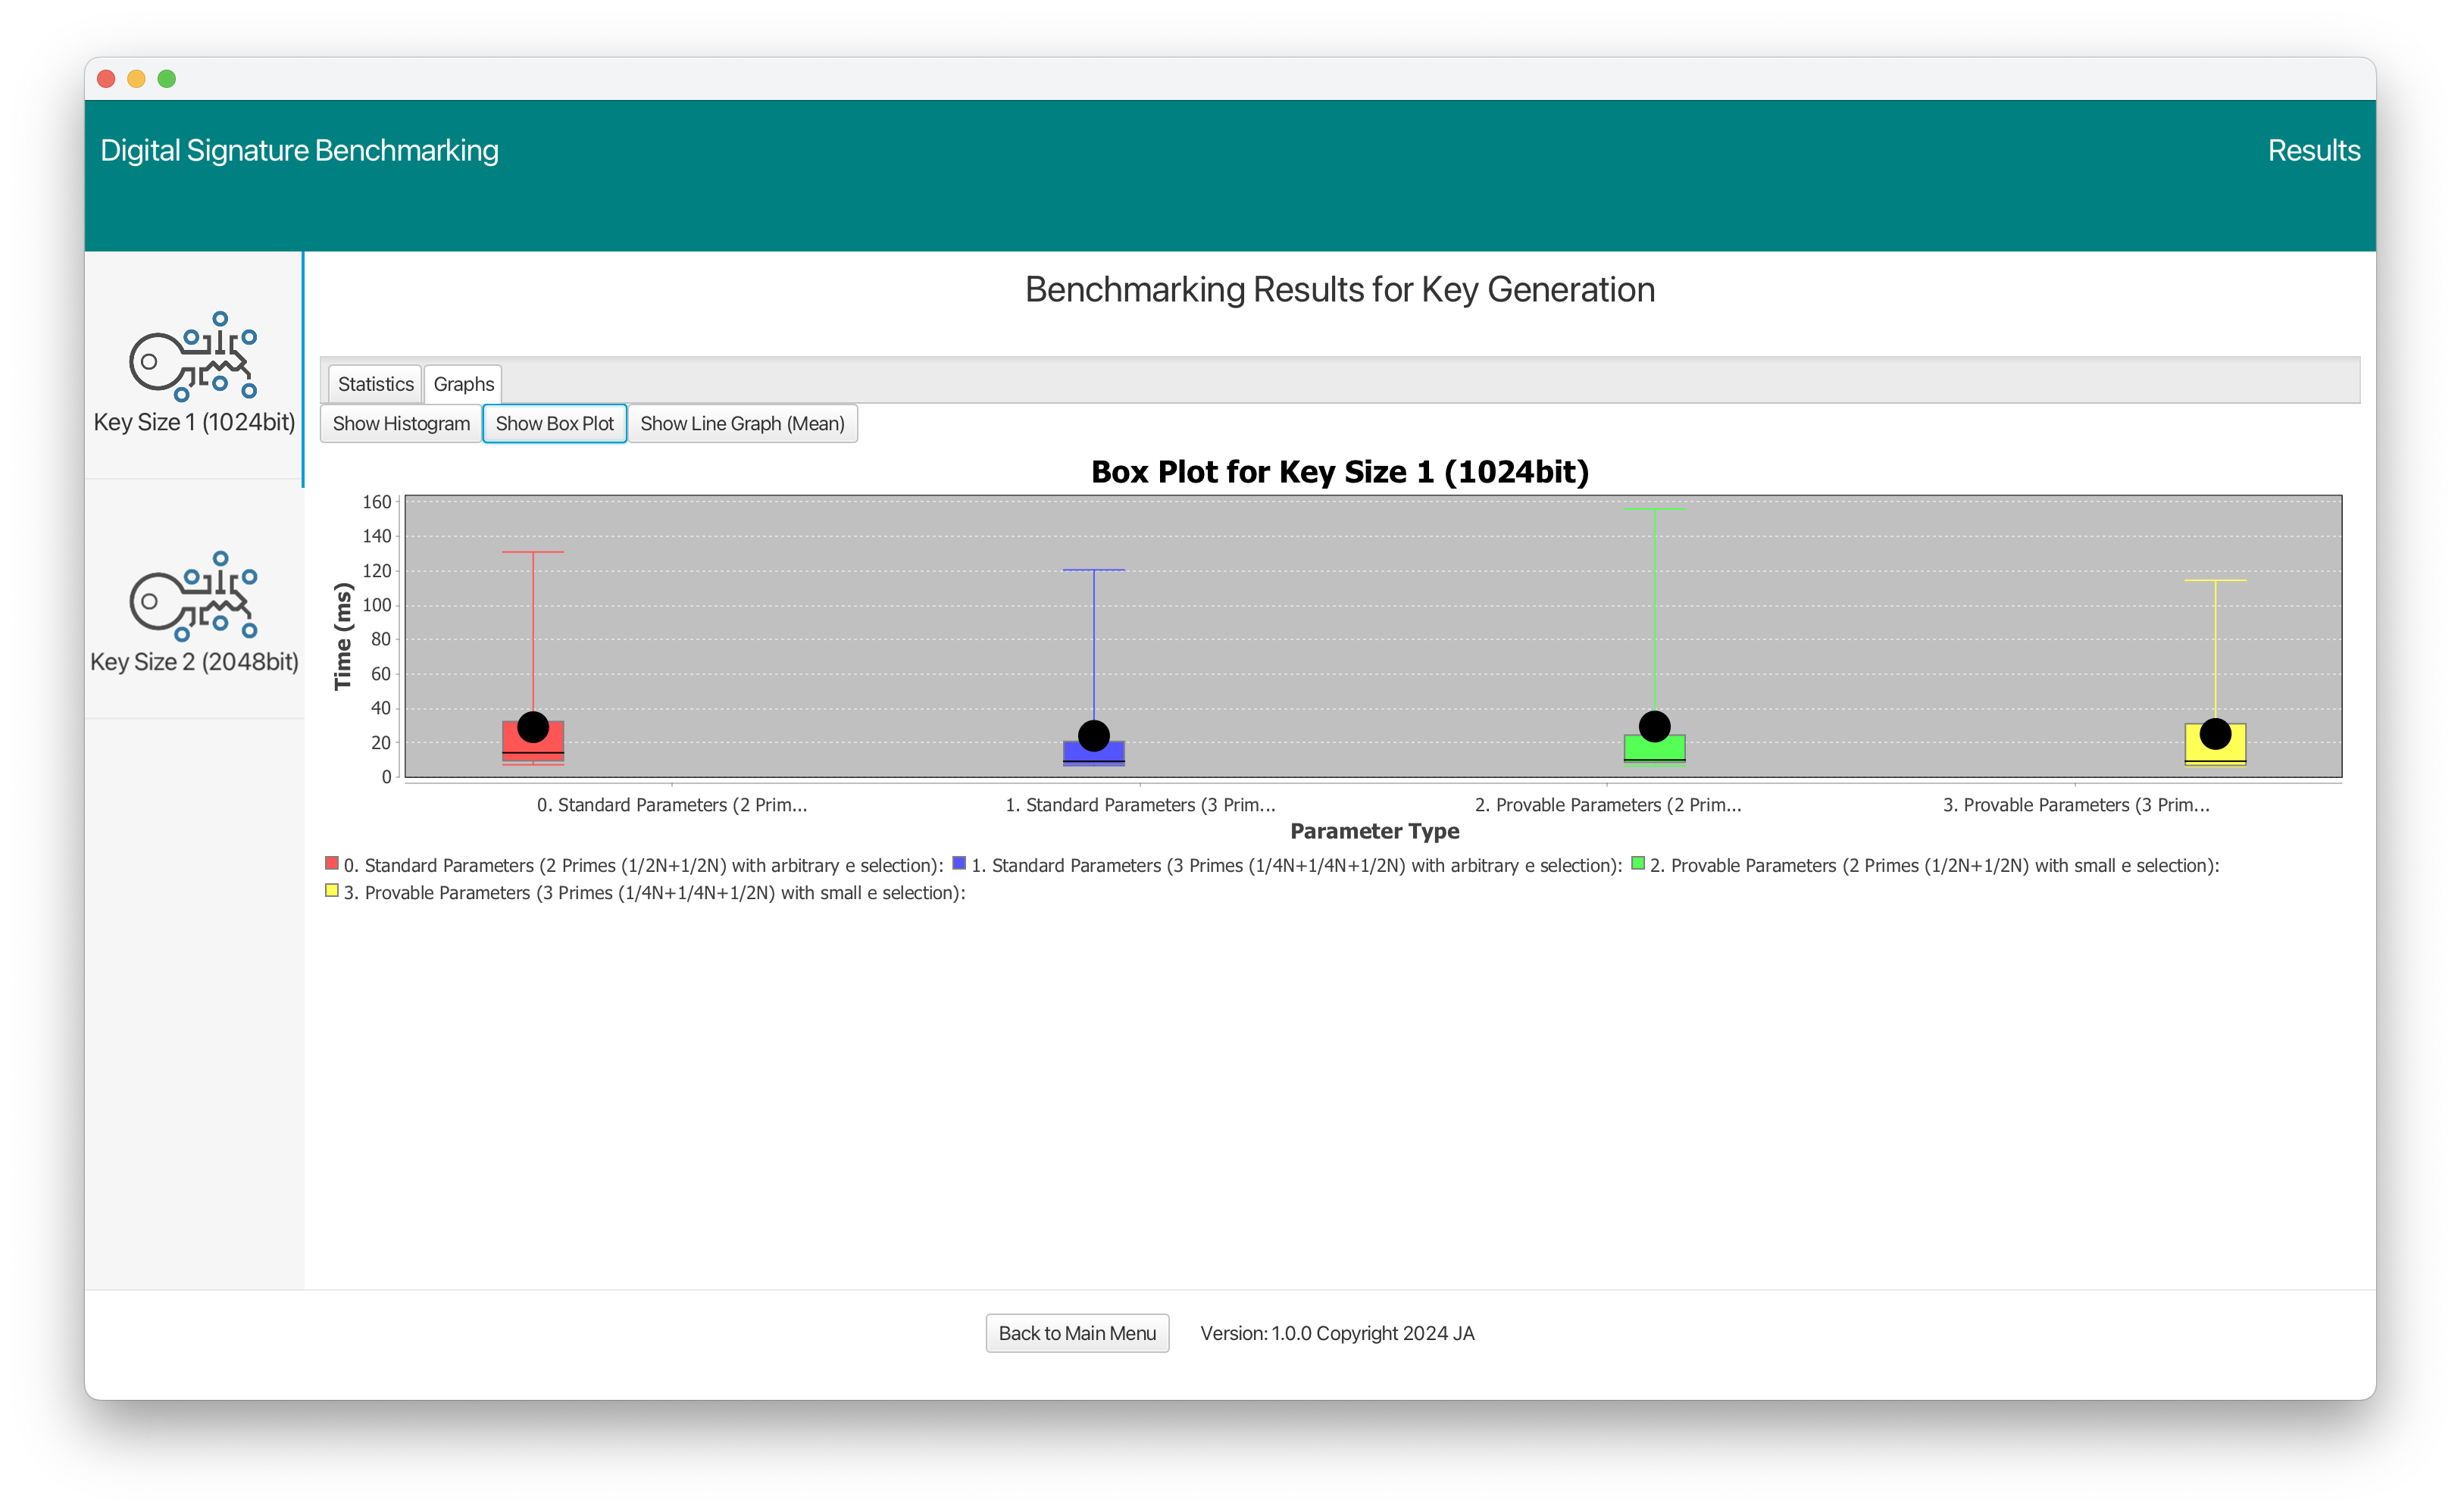
\includegraphics[width=\textwidth]{main_pictures/ui/keyGen/keyGen6.png}} % Adding border here
        \caption{Comparison Benchmarking: Key Generation: Overlaid Box plot graph}
        \label{fig:image2}
    \end{minipage}
     \begin{minipage}{0.7\textwidth}
        \centering
        \fbox{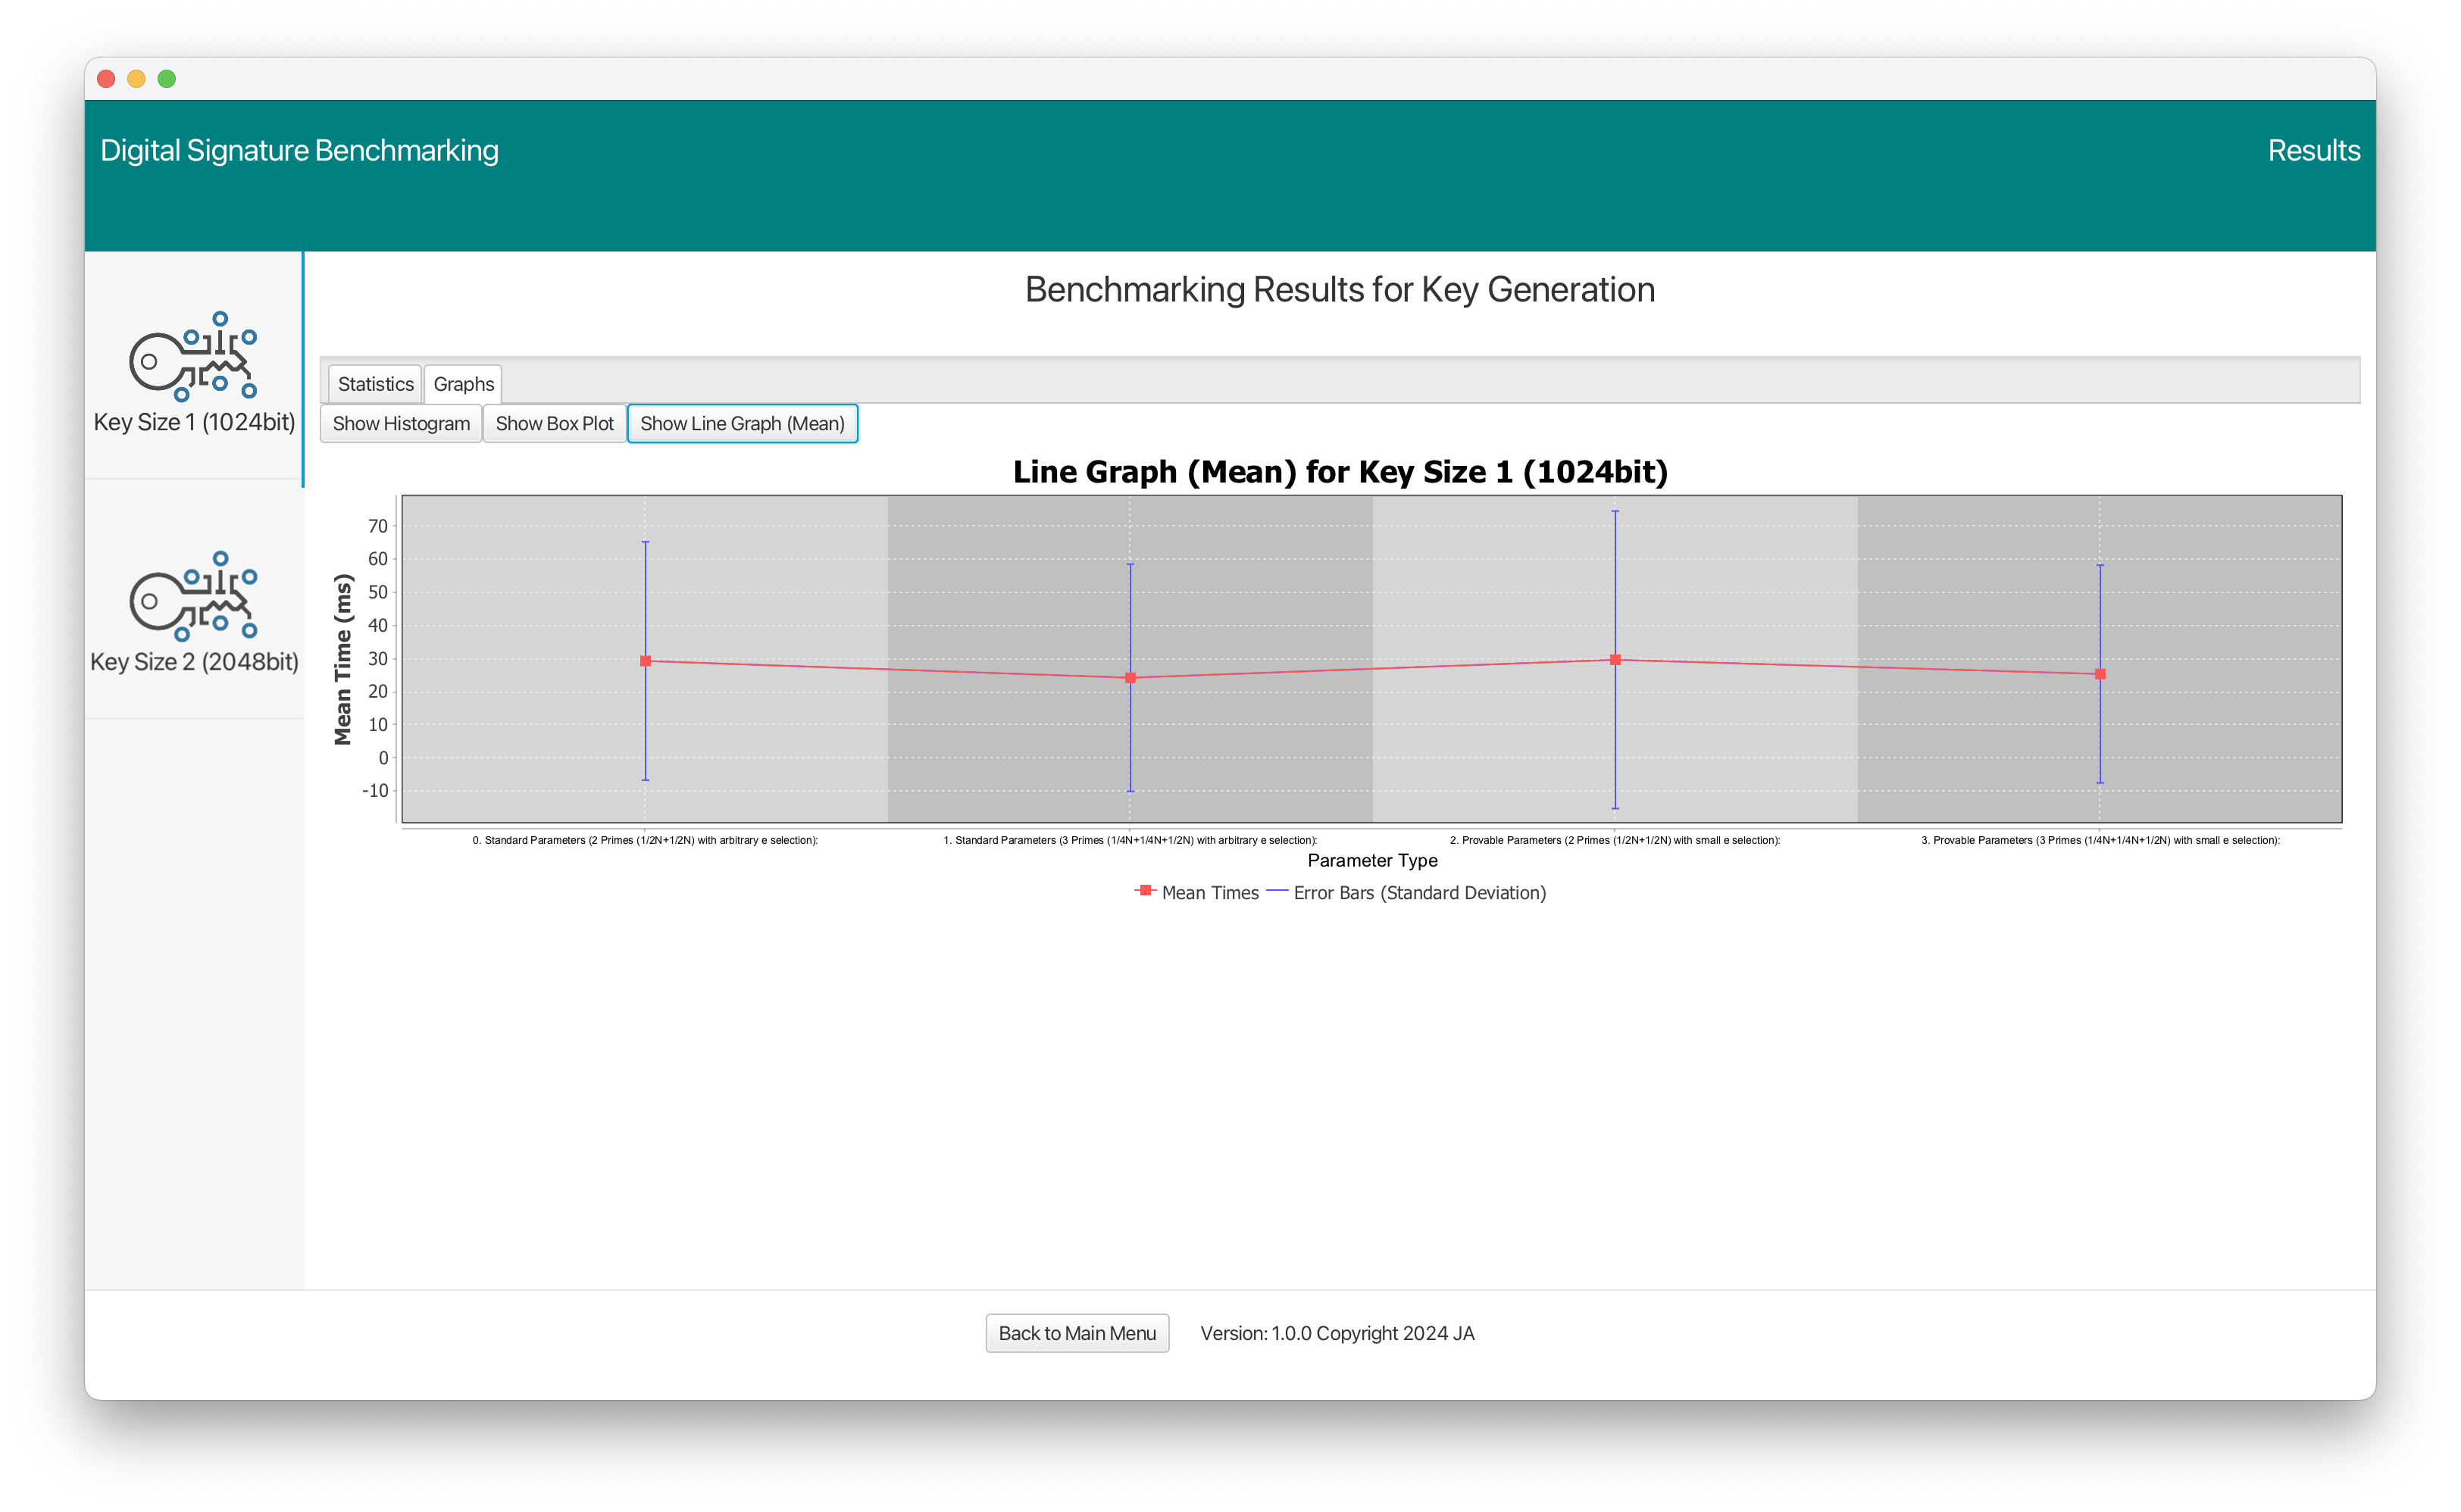
\includegraphics[width=\textwidth]{main_pictures/ui/keyGen/keyGen7.png}} % Adding border here
        \caption{Comparison Benchmarking: Key Generation: Overlaid Line graph for mean times}
        \label{fig:image2}
    \end{minipage}
\end{figure}
An alternative graphical representation of the results can be accessed by navigating to the "Graphs" tab within the central tab pane, where the results table is situated. This tab offers support for three distinct types of graphs, each containing data from all key configurations mapped from the table for easy comparison. These graph types include a stacked histogram, which visualises the distribution of results among configurations for each key size. Additionally, box plots are provided for inferring the distribution of data among configurations. Lastly, mean time line graphs (with error bars for standard deviation) facilitate comparison of average performance and variability among configurations.

\subsection{Signature Generation}
\begin{figure}[H]
    \centering
    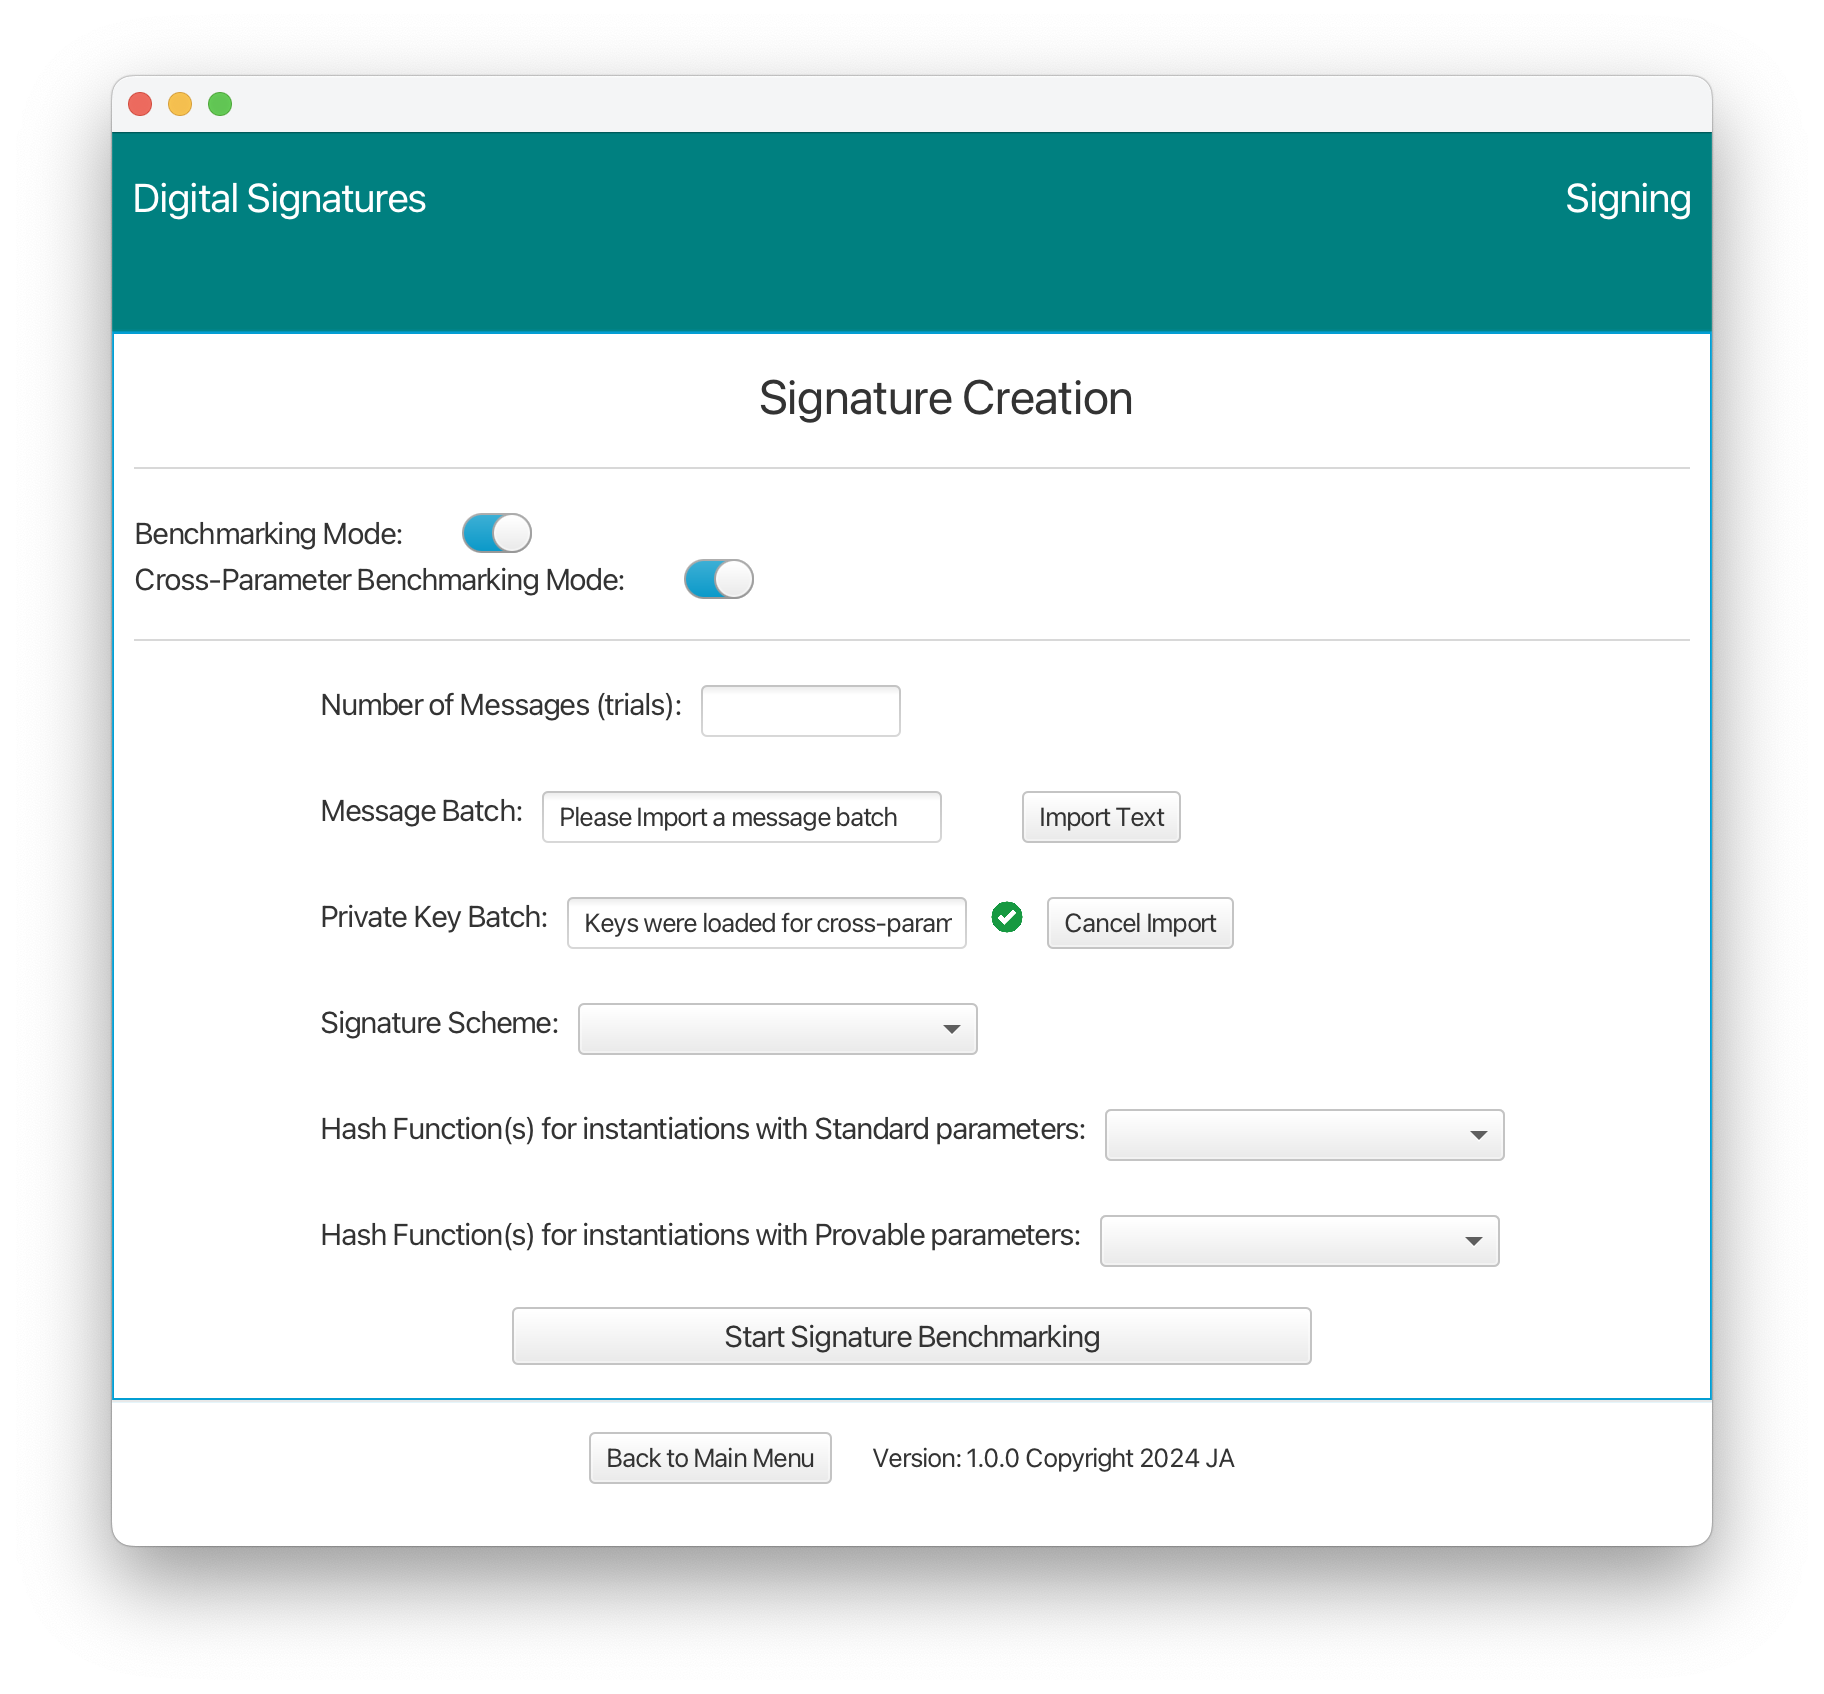
\includegraphics[scale= 0.4]{main_pictures/ui/signing/signing1.png}
    \caption{Signature Generation (Comparison Benchmarking)}
\end{figure}
The initial signature generation screen for comparison benchmarking is activated by completing a key generation benchmarking run in comparison mode. On completion of this, the private key batch (which is also available for export from the results table tab) is preloaded into the signature creation controller. Thus when signature generation option is selected from the main menu, the comparison benchmarking screen is displayed rather than the default benchmarking screen.
This explains the state of cross-parameter benchmarking toggle being set as switched on, as well as, specialised options appearing such as the application displaying a visual indication that a comparison-compatible private key batch was preloaded.



\begin{figure}[H]
    \centering % Center the images
    
    % First image in a minipage
    \begin{minipage}{0.4\textwidth}
        \centering
        \fbox{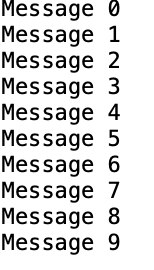
\includegraphics[width=0.4\textwidth]{main_pictures/ui/signing/signing2.png}} % Adding border here
        \caption{Signature Creation (Test message batch (testMessages.txt))}
        \label{fig:image1}
    \end{minipage}
    \hfill % Add some space between the images
    % Second image in a minipage
    \begin{minipage}{0.58\textwidth}
        \centering
        \fbox{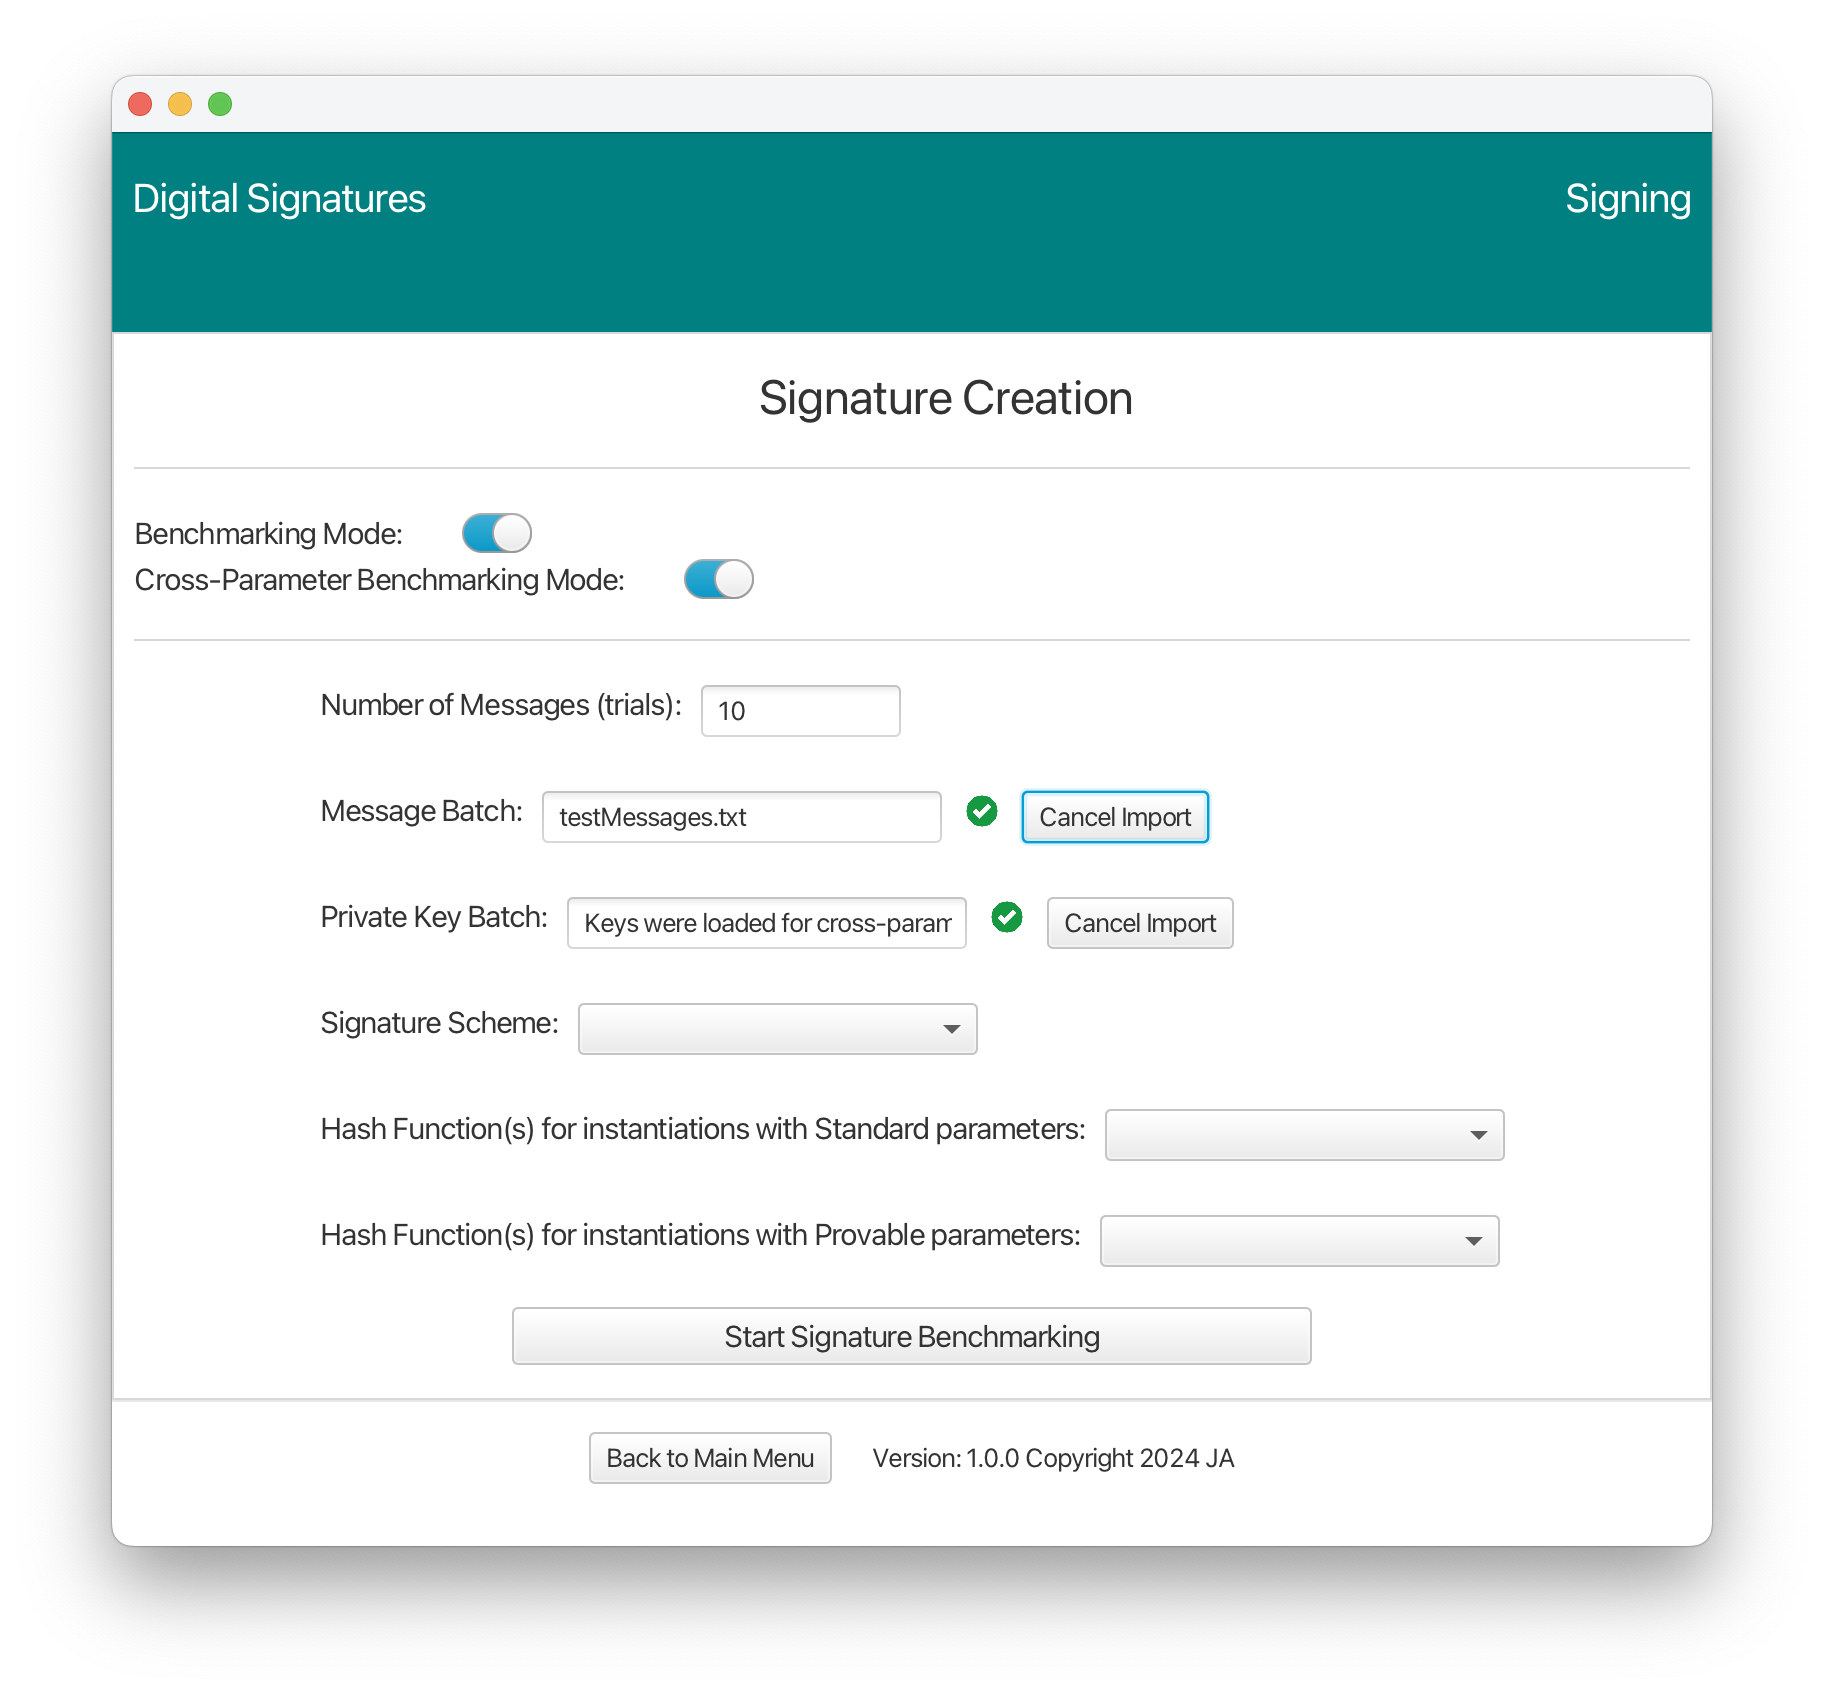
\includegraphics[width=\textwidth]{main_pictures/ui/signing/signing3.png}} % Adding border here
        \caption{Comparison Benchmarking: Signature Creation (Imported message batch)}
        \label{fig:image2}
    \end{minipage}
\end{figure}


The signature creation screen is first organised with a pair of fields related to the importing of a message batch. In the backdrop, the SignatureController class waits to be notified of interaction with the message batch import button. The SignatureController expects the message batch as a non interrupted and new line separated sequence of messages. Upon attempt at an import of a message batch, the SignatureController validates that the number of messages in the message batch candidate, matches the number entered in the adjacently above field, and prevents the import in case of a mismatch. On successful validation it updates the screen with a checkmark indicator that provides visual confirmation that the message batch was successfully imported. The interface also includes a dropdown menu labeled signature scheme giving users the option to select the desired signature scheme  to be applied. 

\begin{figure}[H]
    \centering % Center the images
    
    % First image in a minipage
    \begin{minipage}{0.49\textwidth}
        \centering
        \fbox{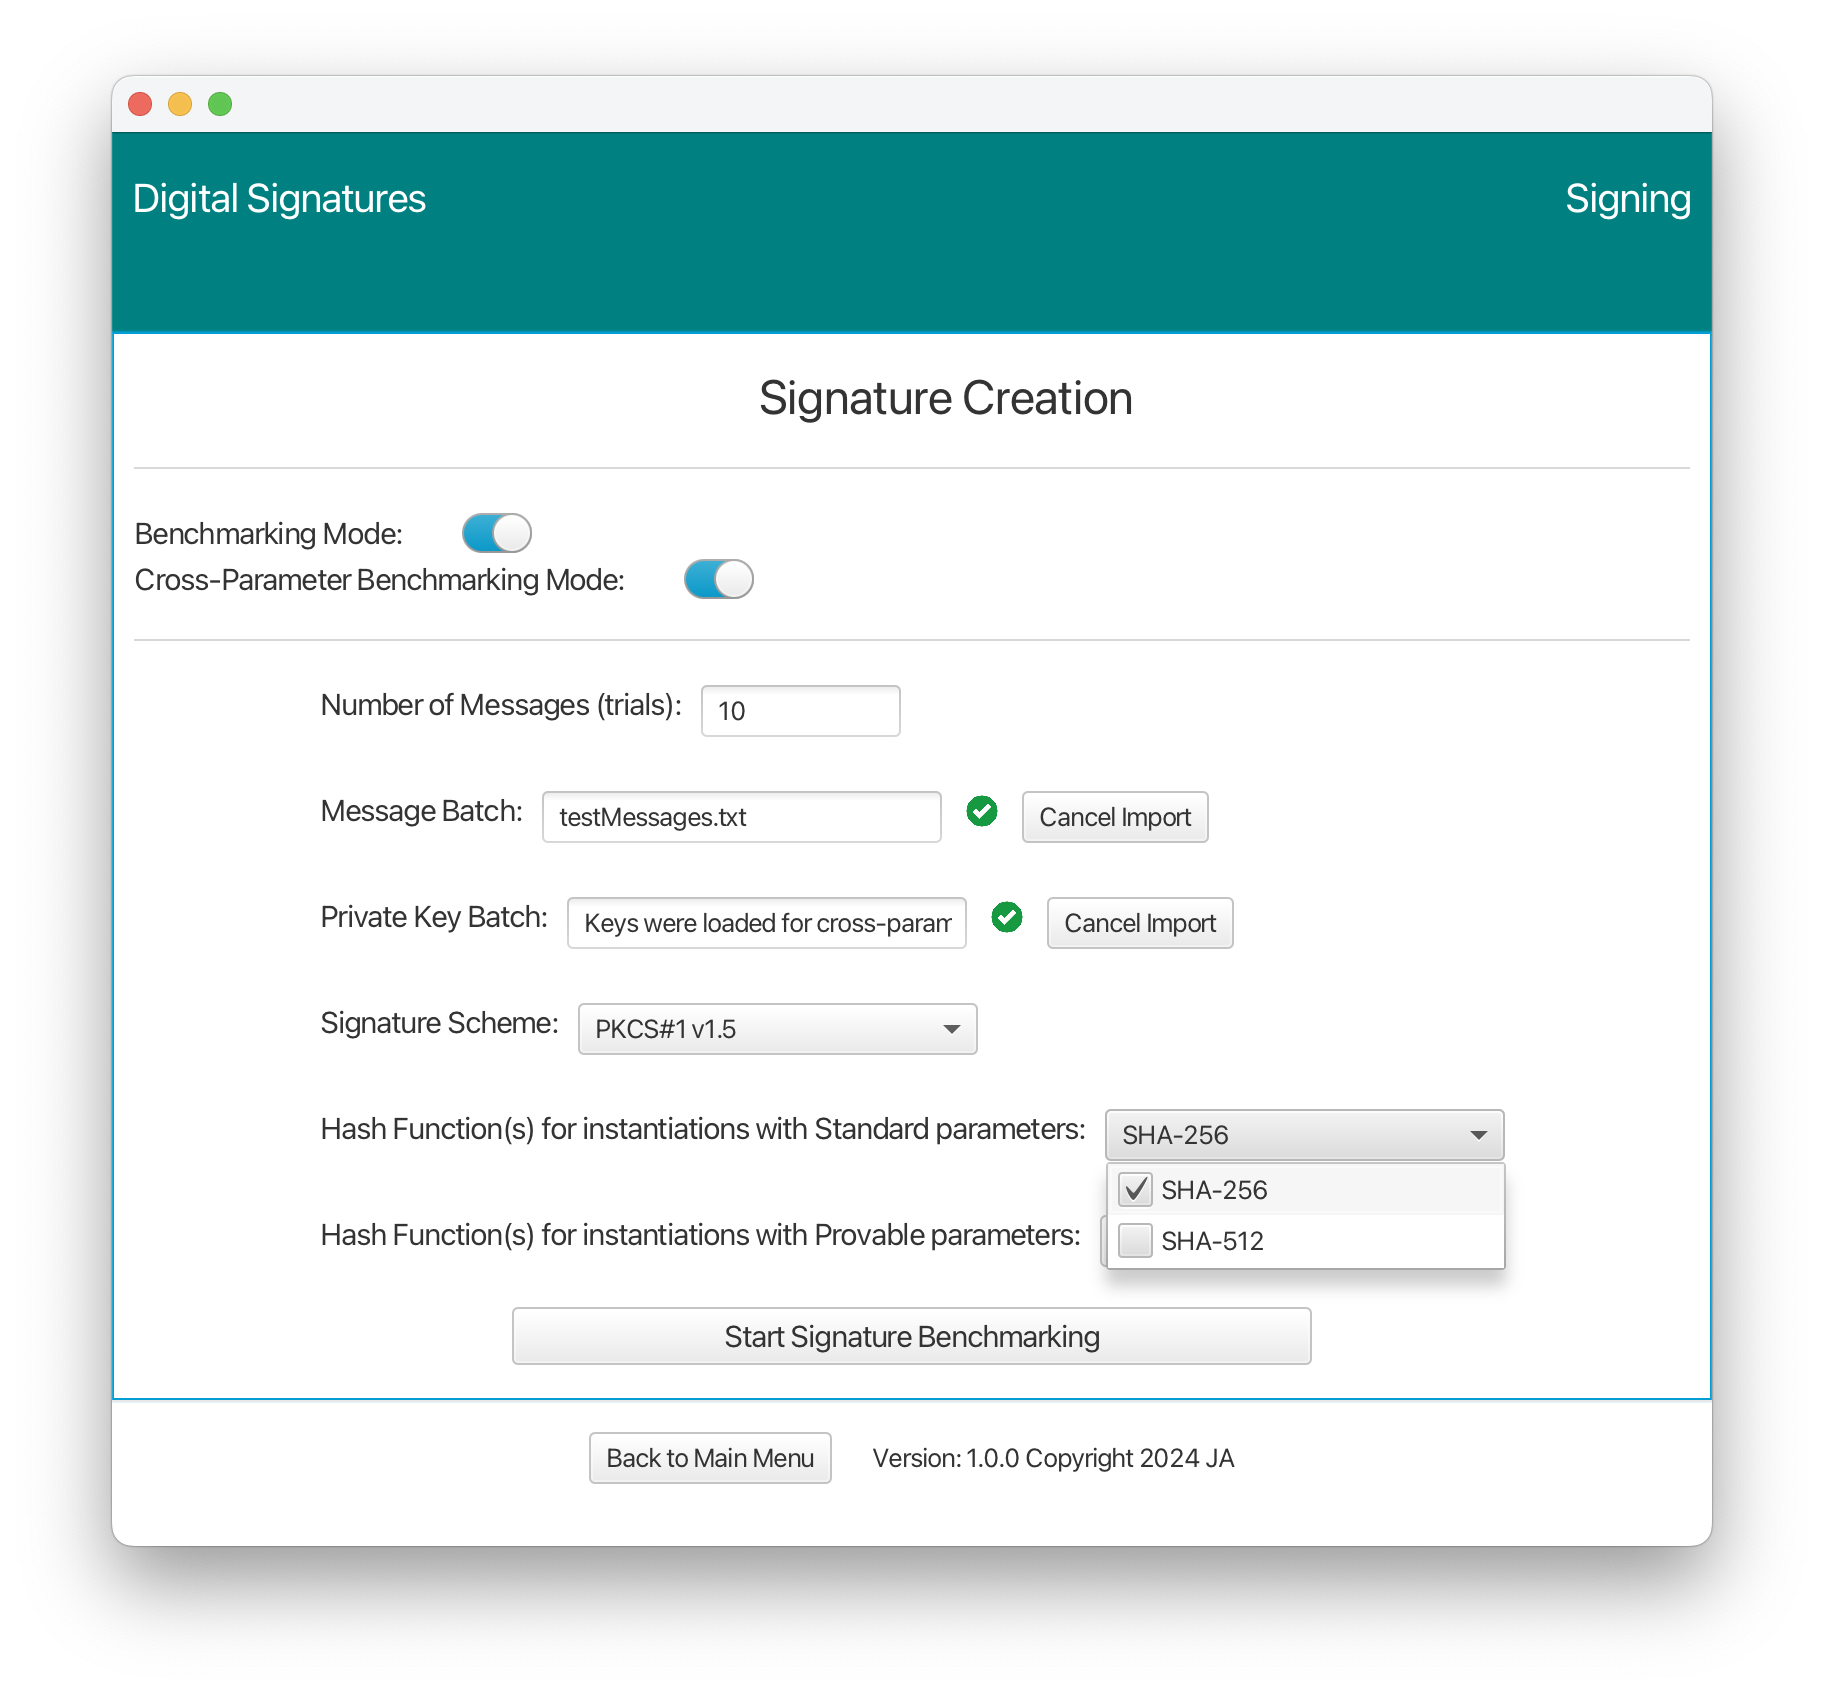
\includegraphics[width=\textwidth]{main_pictures/ui/signing/signing4.png}} % Adding border here
        \caption{Comparison Benchmarking: Signature Creation (Standard Parameter Hash Functions)}
        \label{fig:image1}
    \end{minipage}
    \hfill % Add some space between the images
    % Second image in a minipage
    \begin{minipage}{0.49\textwidth}
        \centering
        \fbox{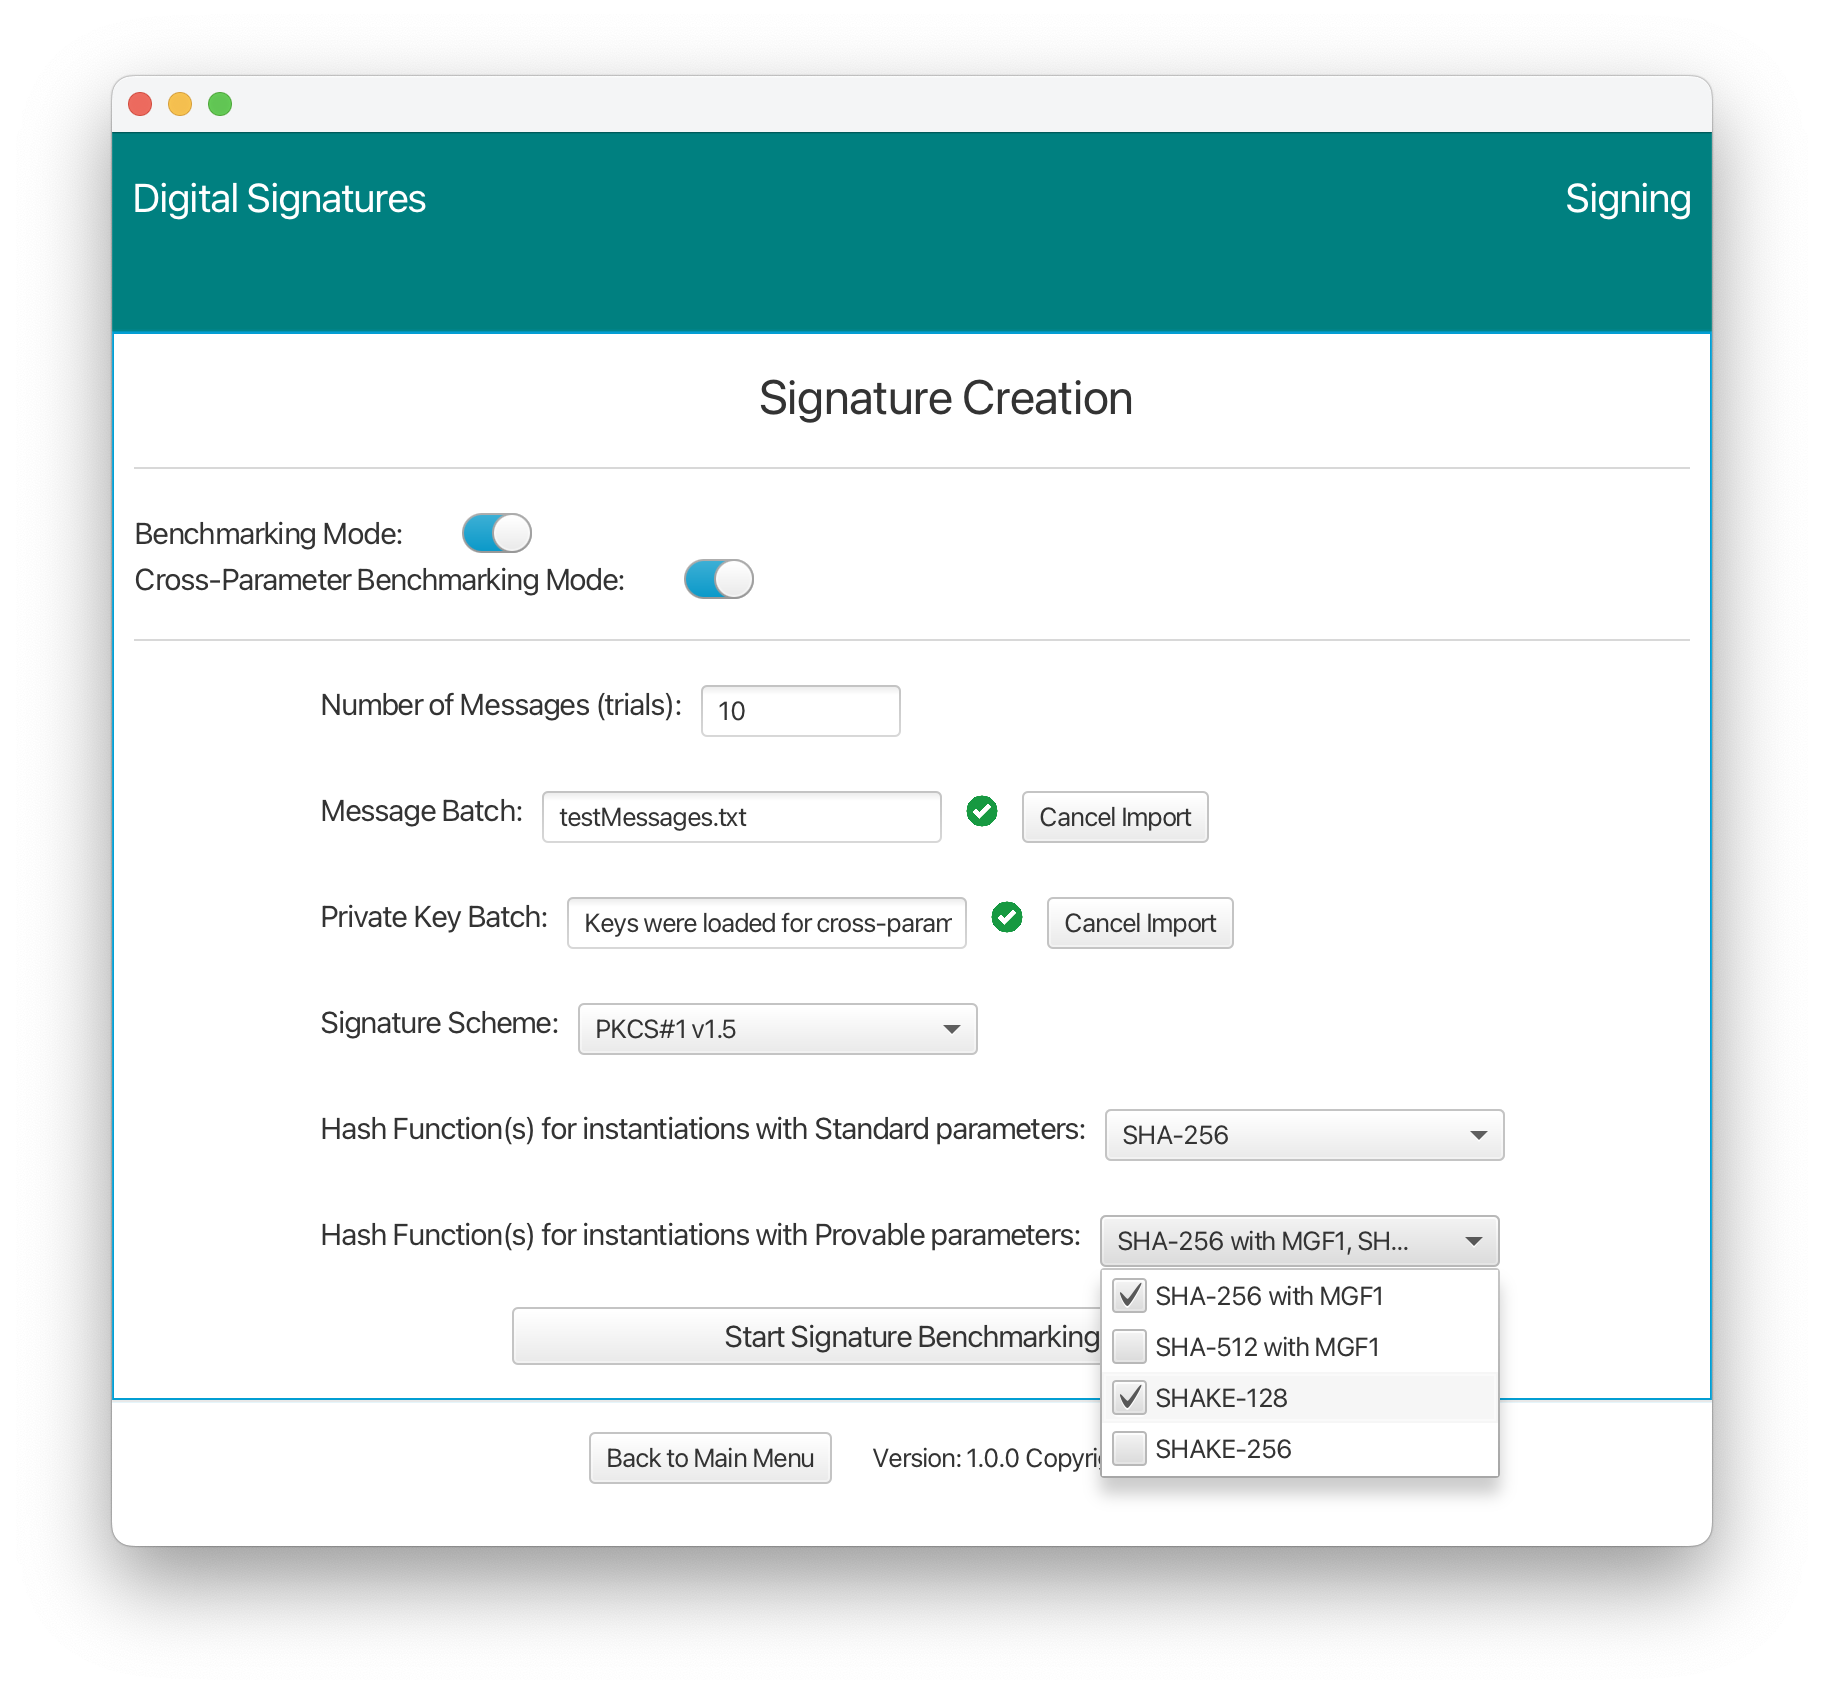
\includegraphics[width=\textwidth]{main_pictures/ui/signing/signing5.png}} % Adding border here
        \caption{Comparison Benchmarking: Signature Creation (Provably Secure Parameter Hash Functions)}
        \label{fig:image2}
    \end{minipage}
      \begin{minipage}{0.55\textwidth}
        \centering
        \fbox{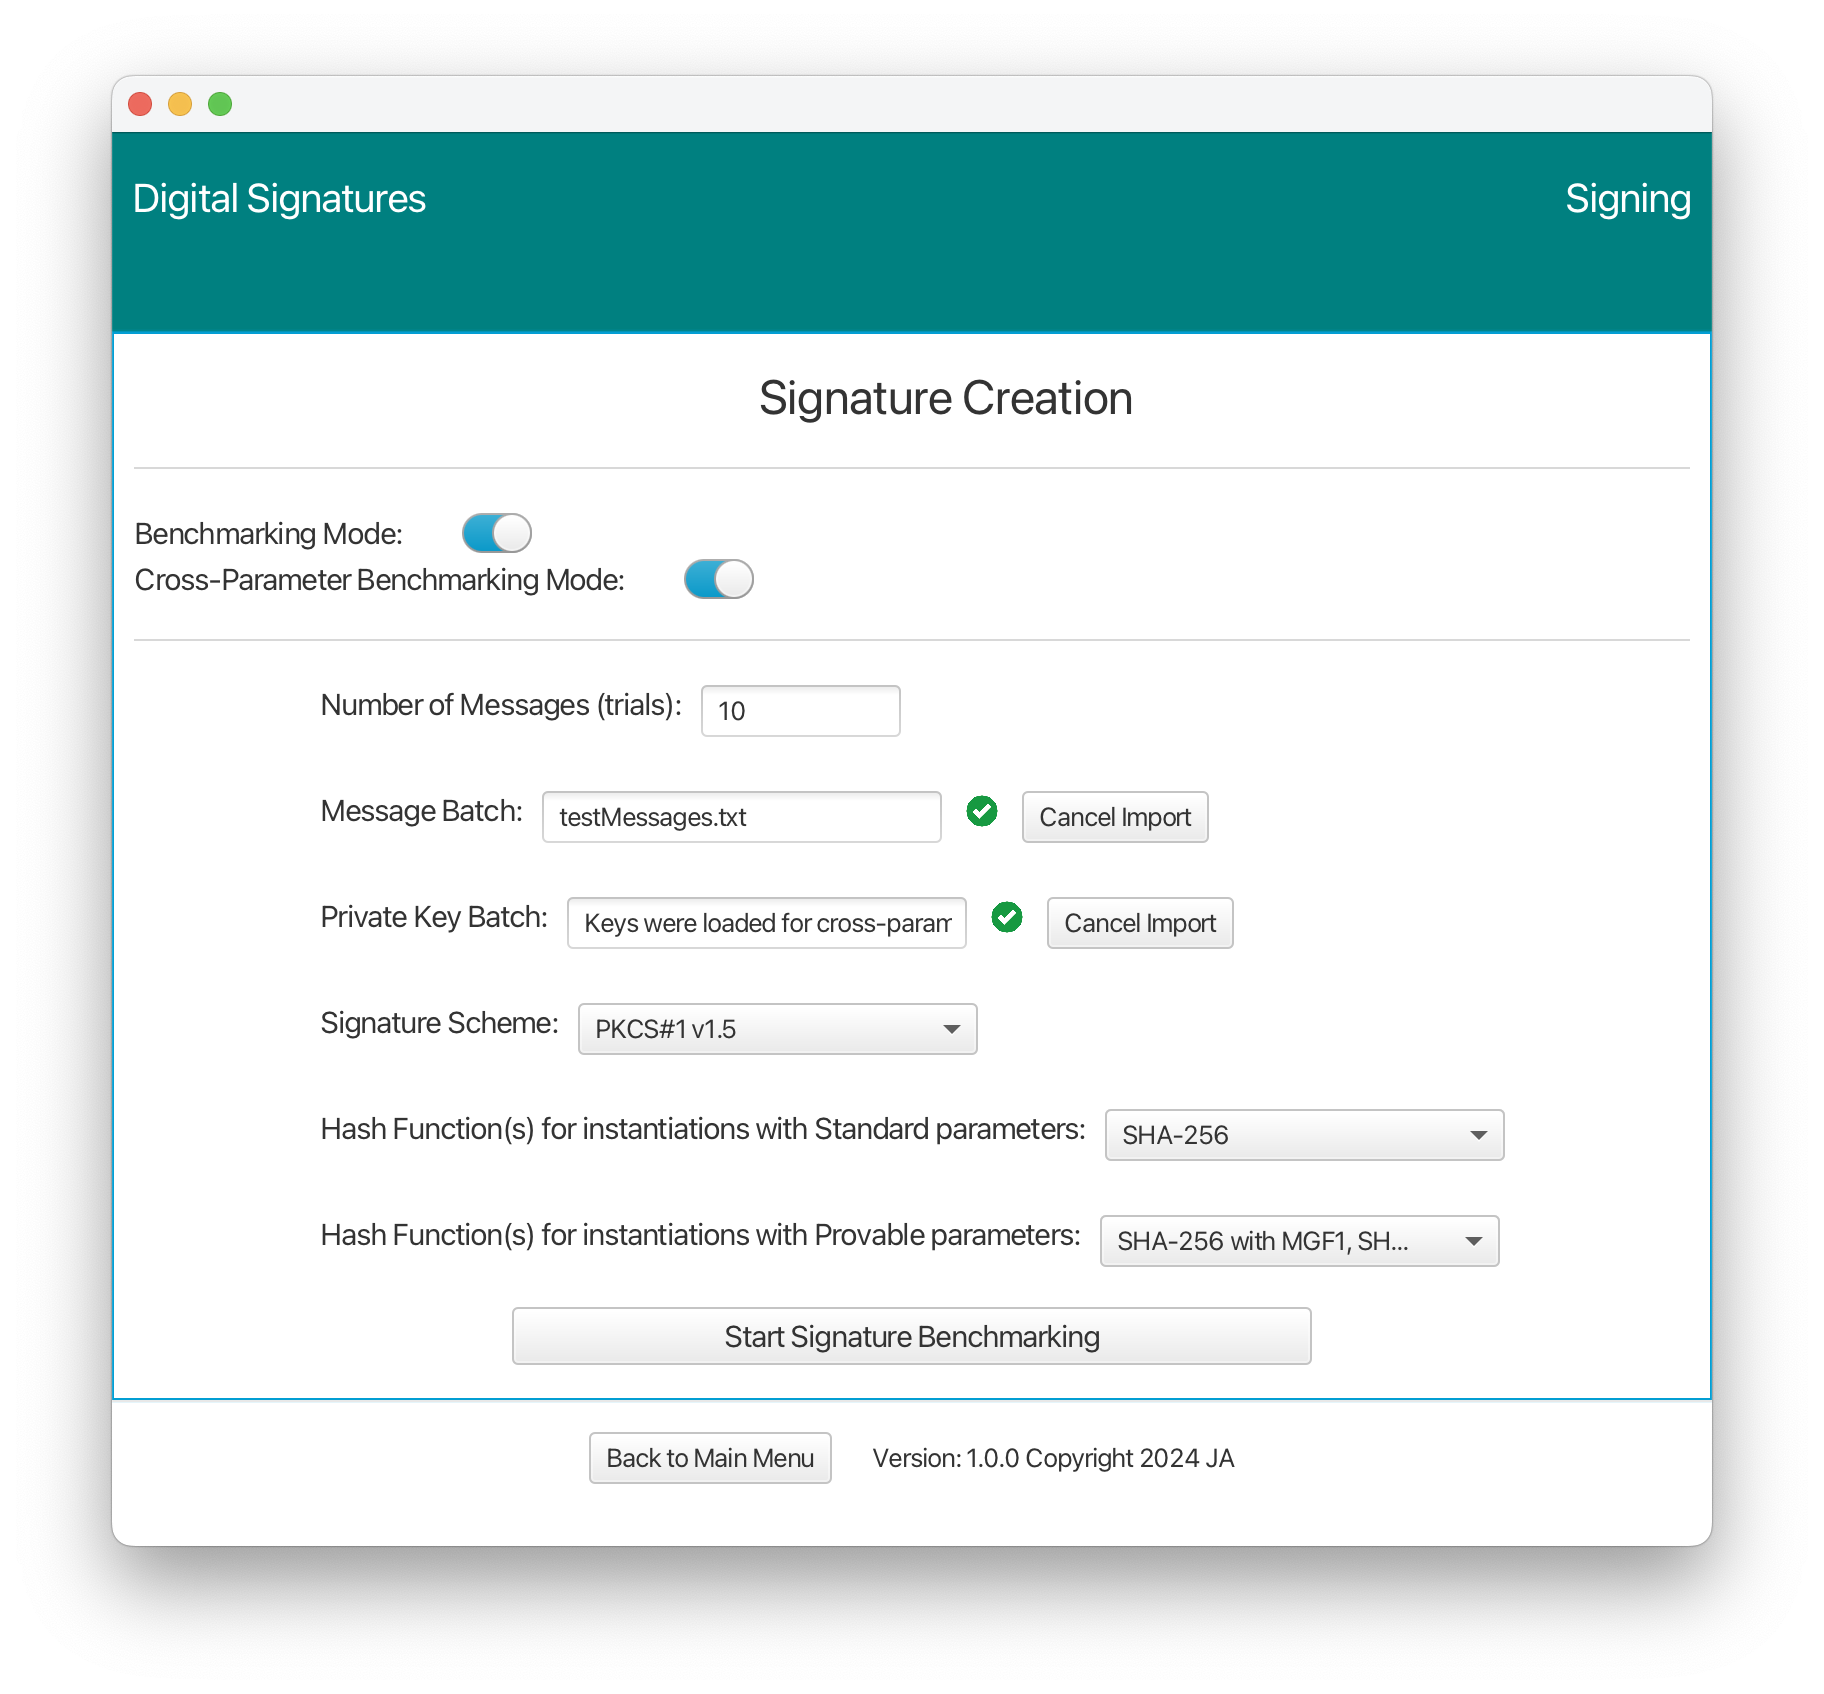
\includegraphics[width=1.2\textwidth]{main_pictures/ui/signing/signing6.png}} % Adding border here
        \caption{Comparison Benchmarking: Signature Creation (All inputs provided)}
        \label{fig:image2}
    \end{minipage}
\end{figure}

In comparison benchmarking mode for signature generation, users select hash functions for standard (fixed-length) and provably secure (variable-length) parameters via a multi-choice drop-down menu. The process involves:

Computing signatures for each selected fixed-length hash function, using the first two key configurations (standard parameters).
Computing signatures for each chosen variable-length hash function, using the last two key configurations (provably secure parameters). This is done sequentially for each key size.

The "Start Signature Benchmarking" button initiates a series of checks and processes. The SignatureController validates the message batch, private key batch, signature scheme, and hash function choices. If any issues are detected, an alert prompts the user to correct them.

Upon passing these checks, the SignatureModel executes the benchmarking task, creating a batch of signatures for the message batch using the designated signature scheme and hash function-key combinations. A progress bar indicates progress in real time.


\begin{comment}
Selection of hash functions for signature generation in comparison benchmarking mode is presented on a per-group basis, with relevant hash function options displayed to enable instantiation of the selected scheme with standard parameters (e.g., fixed-length hash functions) and provably secure parameters (e.g., variable-length hash functions).

The mechanism for selecting the hash function(s) for each group is via a multi-choice drop-down menu. This entails repeating the computation of signatures for the full message set and the first two key configurations (e.g., standard parameter keys) for each of the fixed-length hash functions chosen. Similarly, the computation of signatures for the full message set and the final two key configurations (e.g., provably secure keys) will be repeated for each of the variable-length hash functions selected from the provably secure drop-down menu. This process is enumerated sequentially for each key size.

Upon selection of the "Start Signature Benchmarking" button, a chain of validation and execution steps are executed. The SignatureController first verifies that the message batch input, private key batch, signature scheme and hash function selections are valid and present. Should any discrepancies arise during this stage, the interface promptly presents an alert, informing the user of the necessary corrective measures.


Once the preliminary checks are met, the SignatureModel assumes control to perform the benchmarking task. It computes a batch of  signatures for the provided message batch with the private key batch using the selected signature scheme and relevant hash function to key combinations. A progress bar is displayed for a length of time spanning the duration of the task allowing for real-time indication of progress.
\end{comment}

\begin{figure}[H]
    \centering
    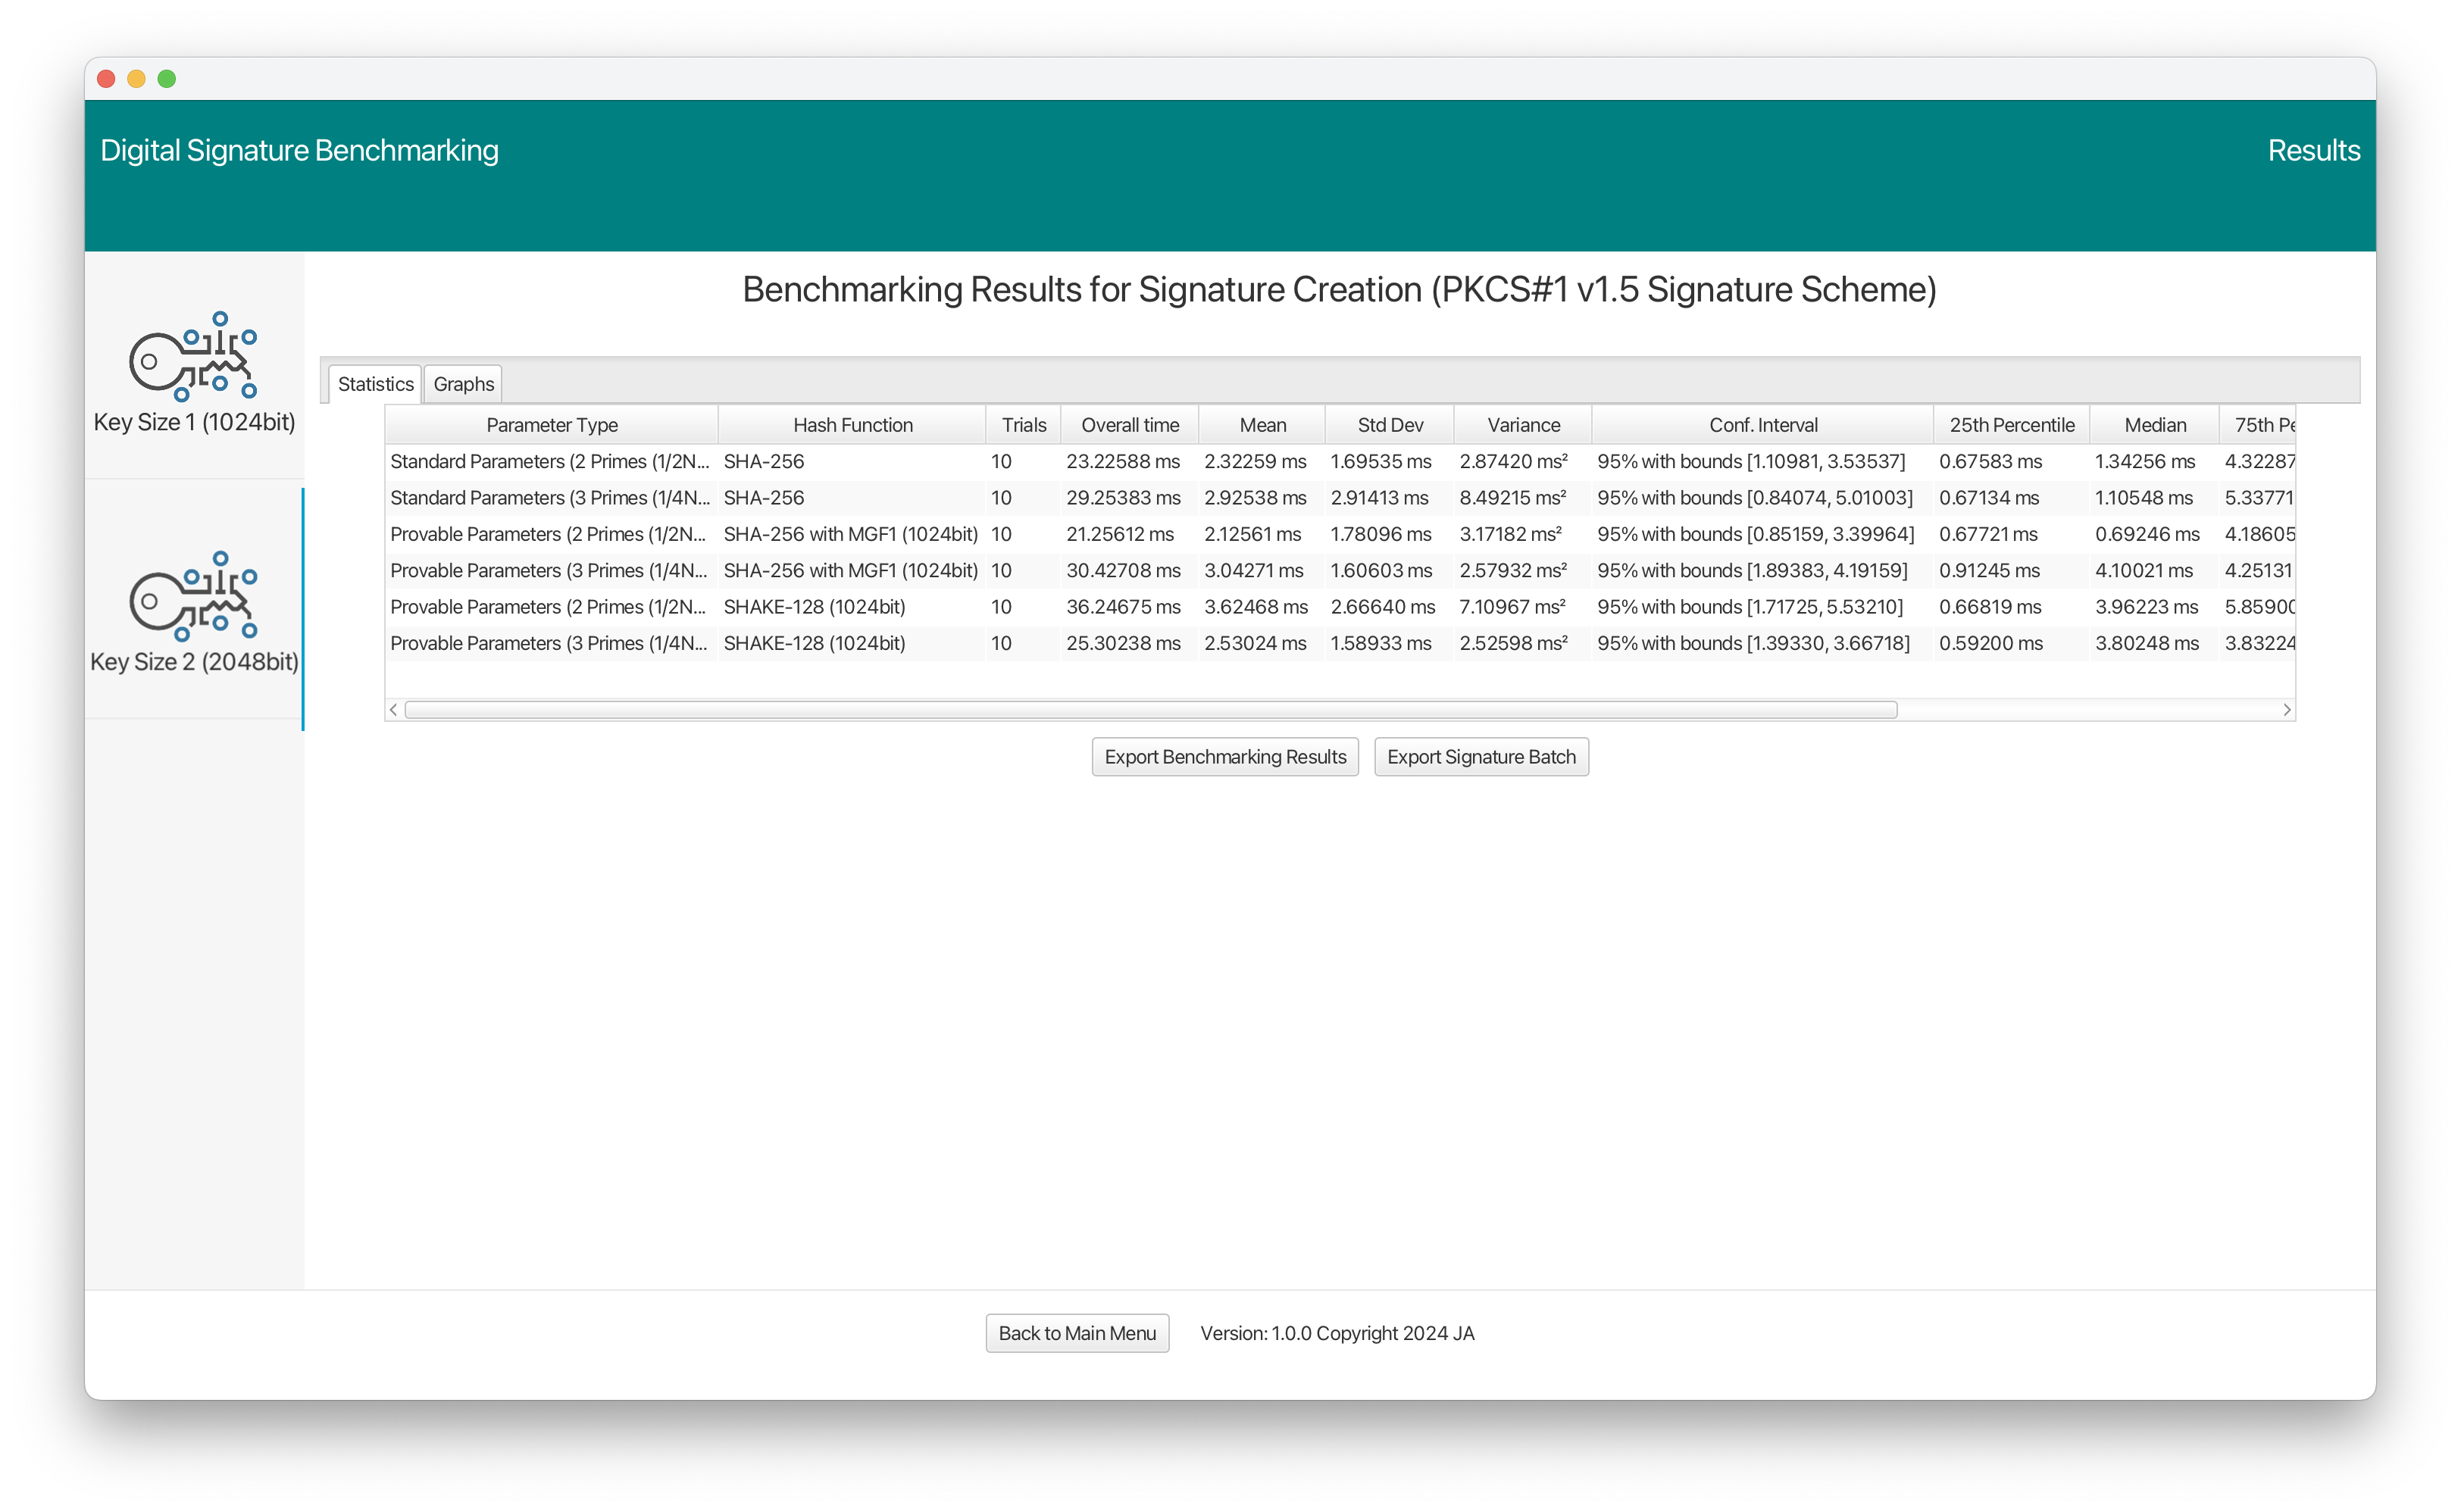
\includegraphics[scale= 0.325]{main_pictures/ui/signing/signing7-2.png}
    \caption{Comparison Benchmarking: Signature Generation (Results Screen)}
\end{figure}

After completing signature generation benchmarking, the ResultsController displays the results. The results screen features a side pane with tabs for each key size entered. Each tab reveals a results table displaying statistical metrics for all hash function-key combinations.

The table format aligns with the user's hash function choices. For example, selecting one hash function (e.g., SHA-256) for standard parameters results in two rows for this set. For provably secure parameters, if two functions like SHA-256 with MGF1 and SHAKE-128 are chosen, they each generate two rows, totalling four rows. This format leads to six rows per key size, each row representing signature computations for the full message batch.

Below the table, options are available to export benchmarking results and signature batches for each key size. The exported signature batch aligns with the key configurations and hash function combinations used, covering all key sizes in a single file.



%TC:ignore
\textbf{Comparison Benchmarking: Signature Generation Results Screen Graphs}
%TC:endignore

\begin{figure}[H]
    \centering % Center the images
    
    % First image in a minipage
    \begin{minipage}{0.7\textwidth}
        \centering
        \fbox{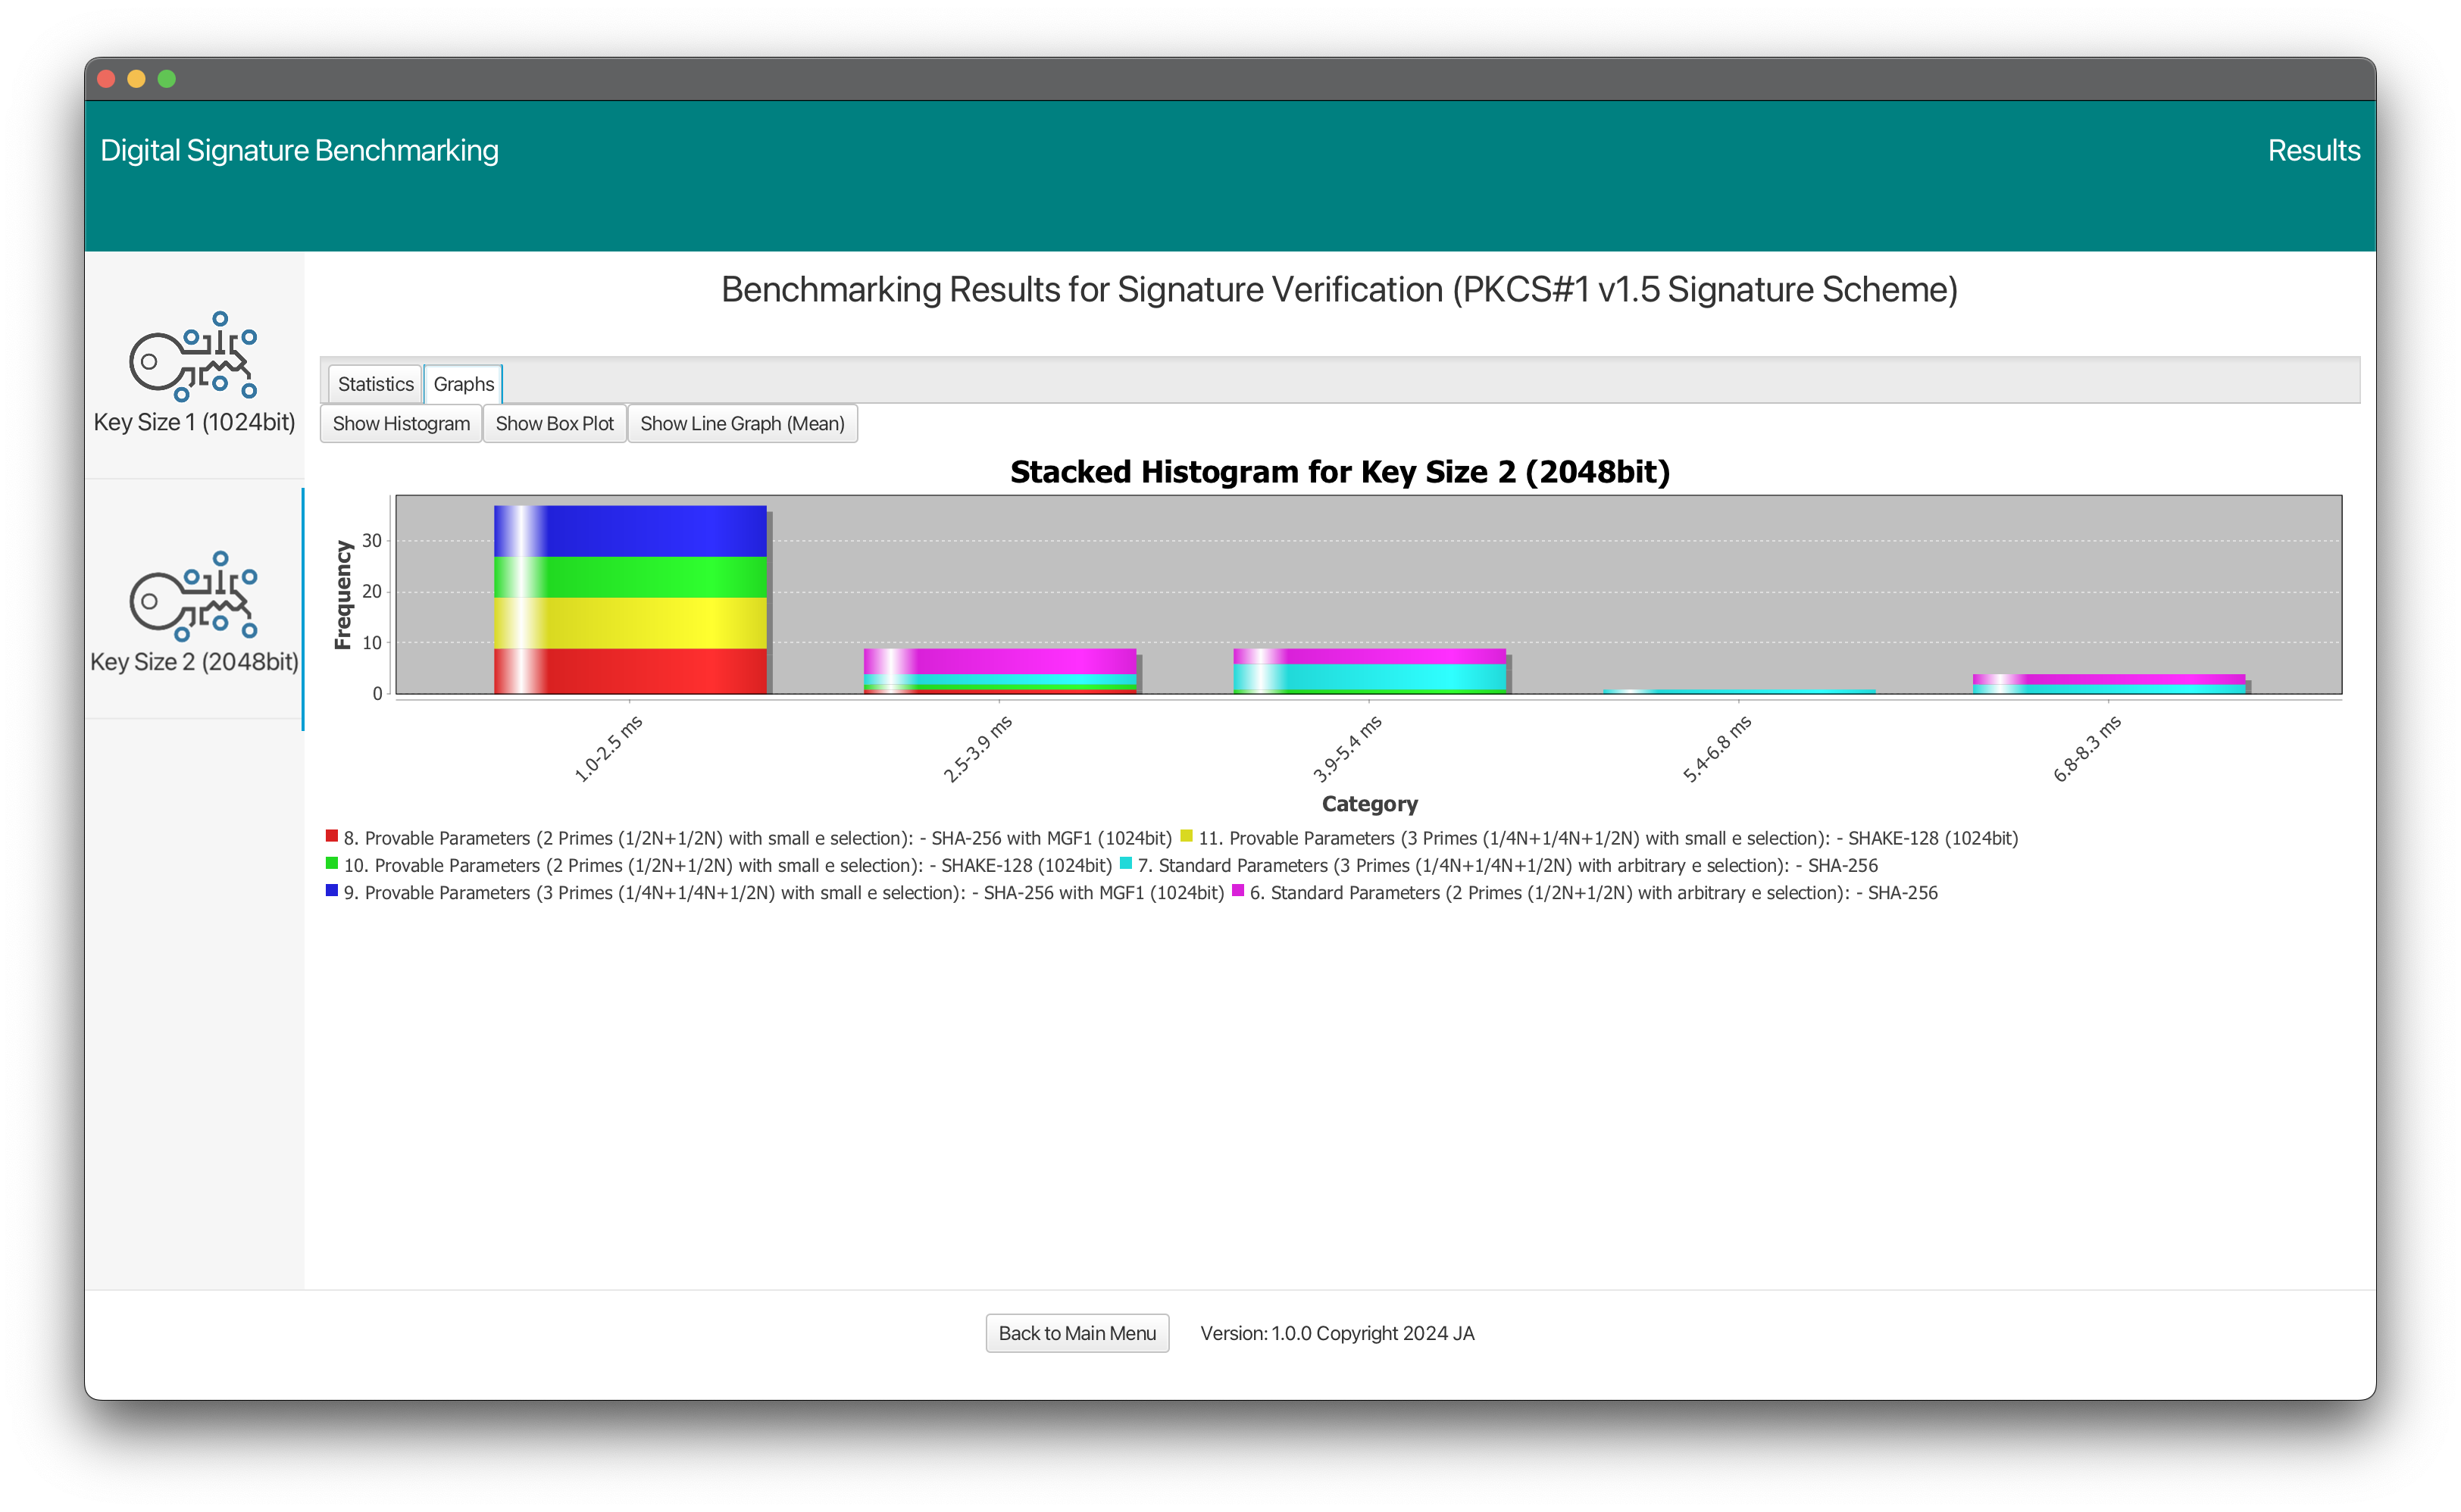
\includegraphics[width=\textwidth]{main_pictures/ui/signing/signing8-2.png}} % Adding border here
        \caption{Comparison Benchmarking: Signature Generation: Overlaid Histogram}
        \label{fig:image1}
    \end{minipage}
    \hfill % Add some space between the images
    % Second image in a minipage
    \begin{minipage}{0.7\textwidth}
        \centering
        \fbox{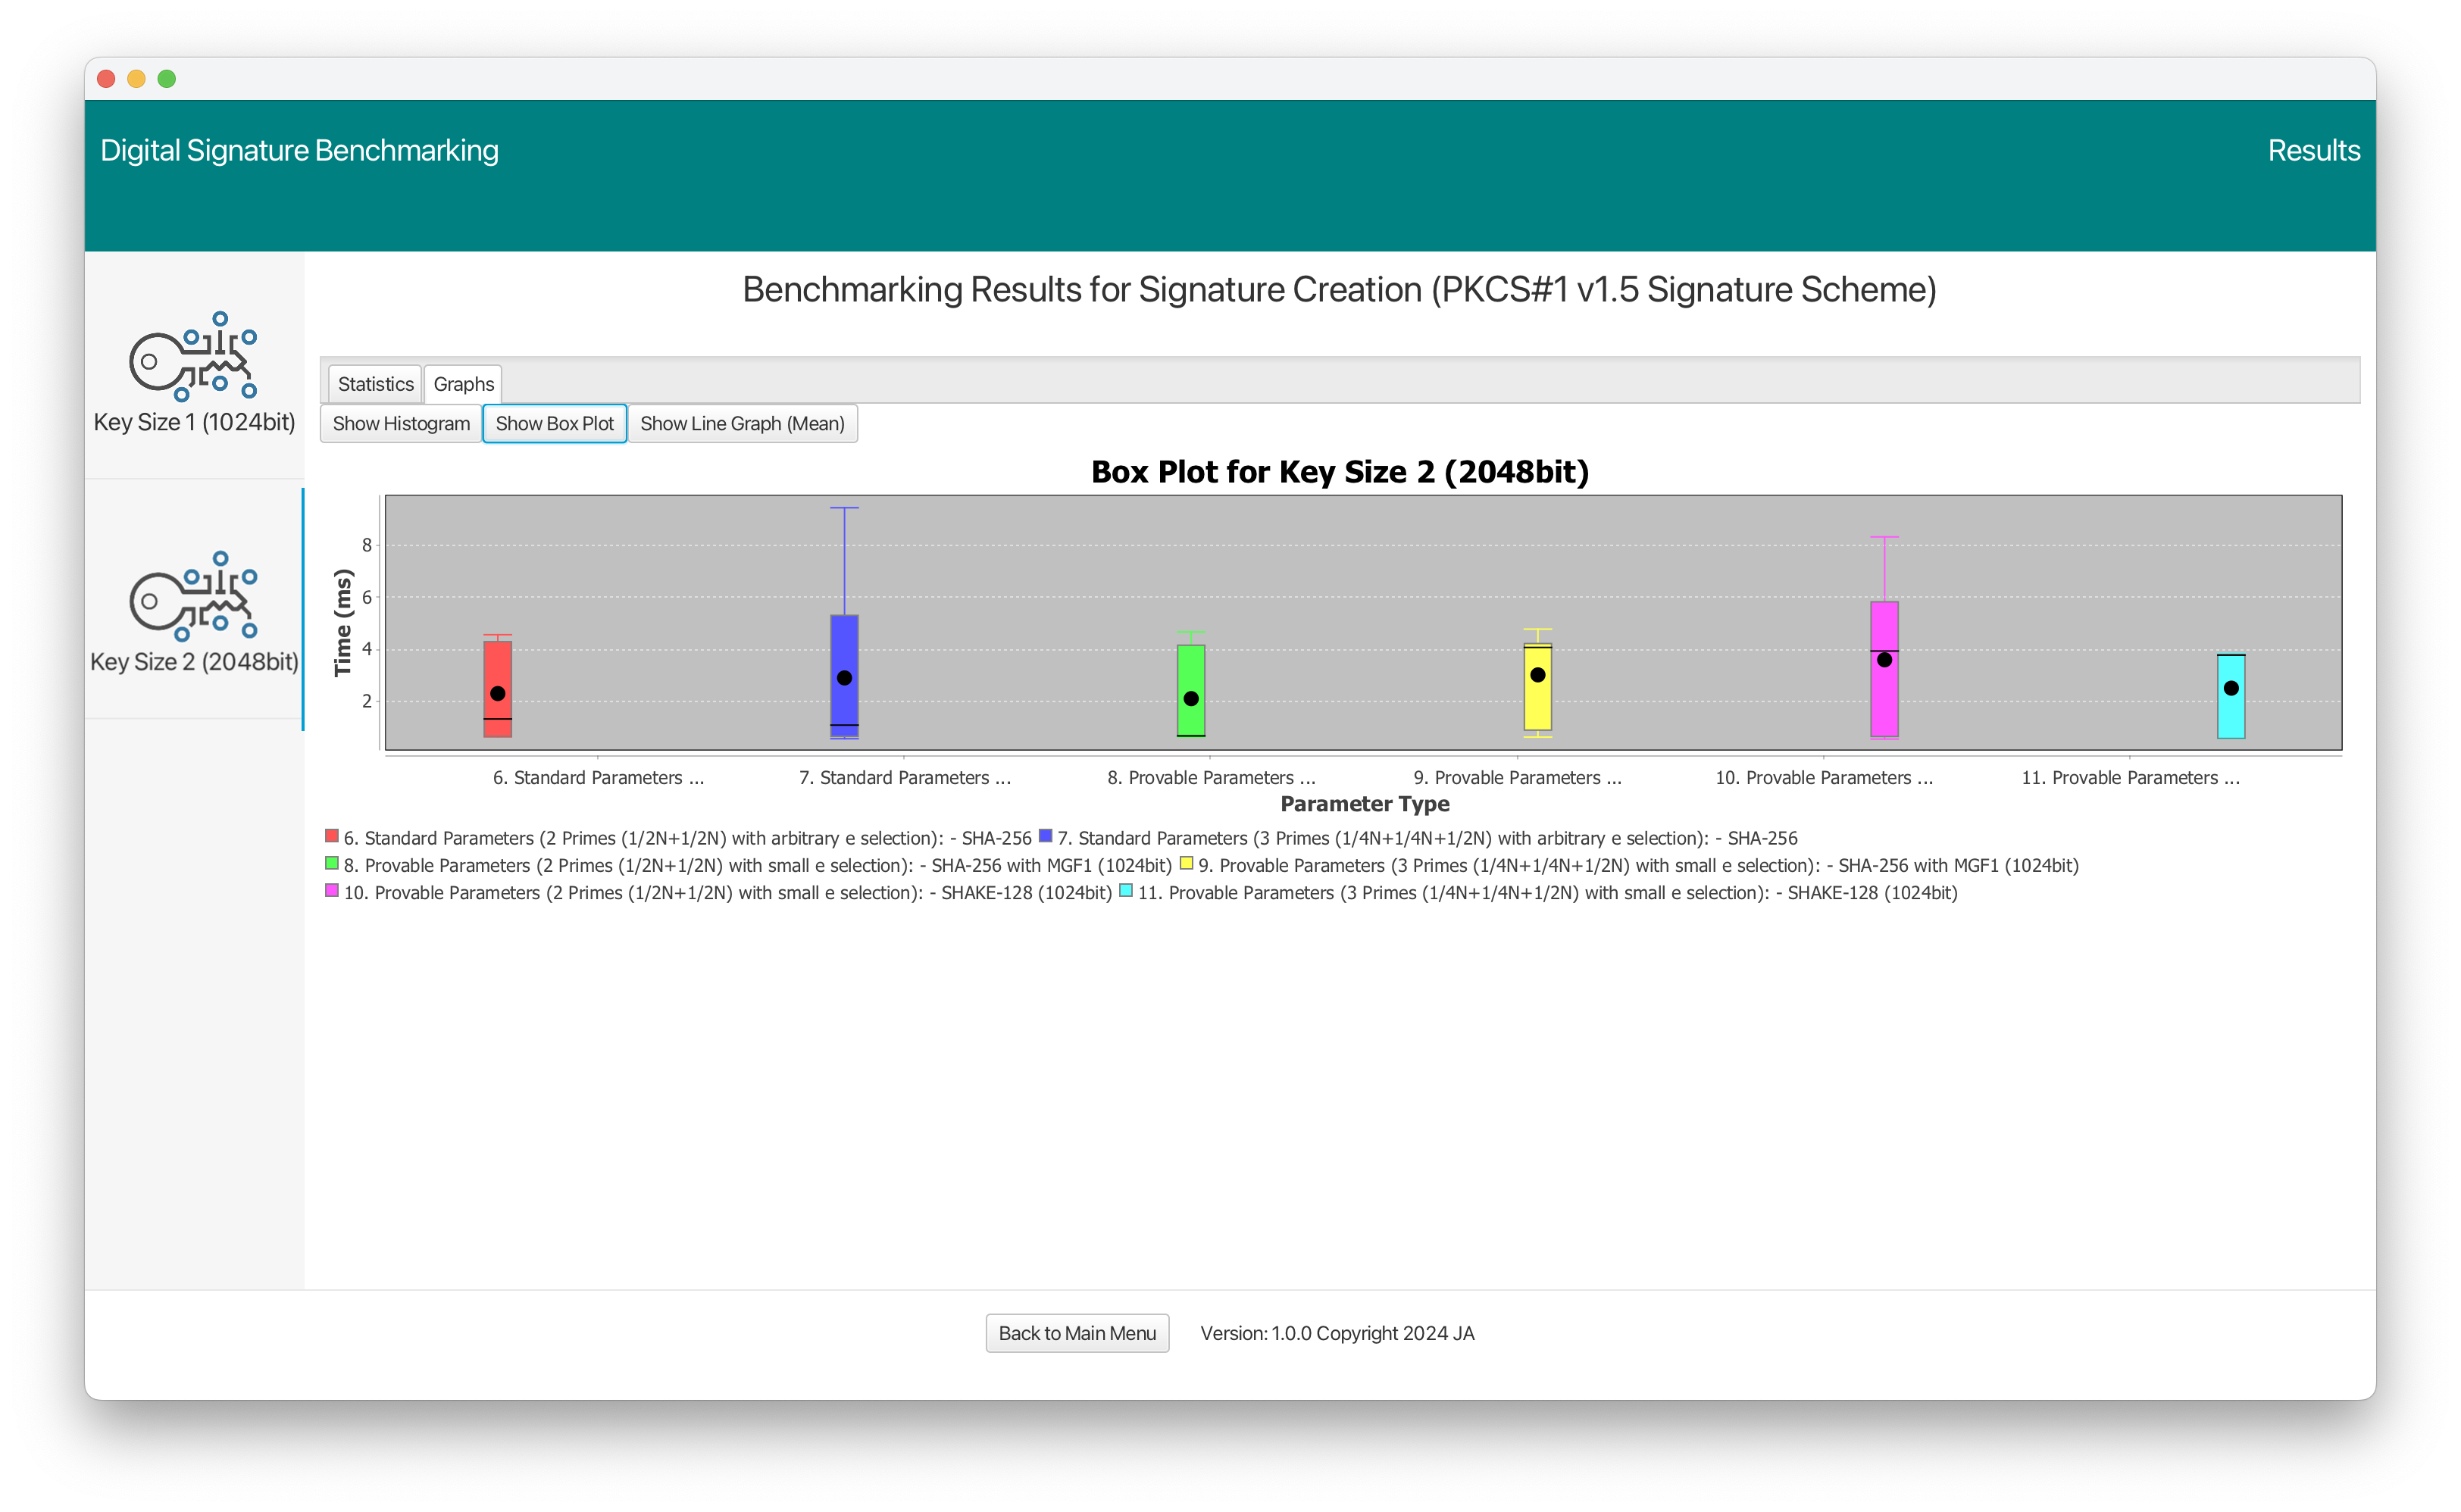
\includegraphics[width=\textwidth]{main_pictures/ui/signing/signing9-2.png}} % Adding border here
        \caption{Comparison Benchmarking: Signature Generation: Overlaid Box plot graph}
        \label{fig:image2}
    \end{minipage}
        \begin{minipage}{0.7\textwidth}
        \centering
        \fbox{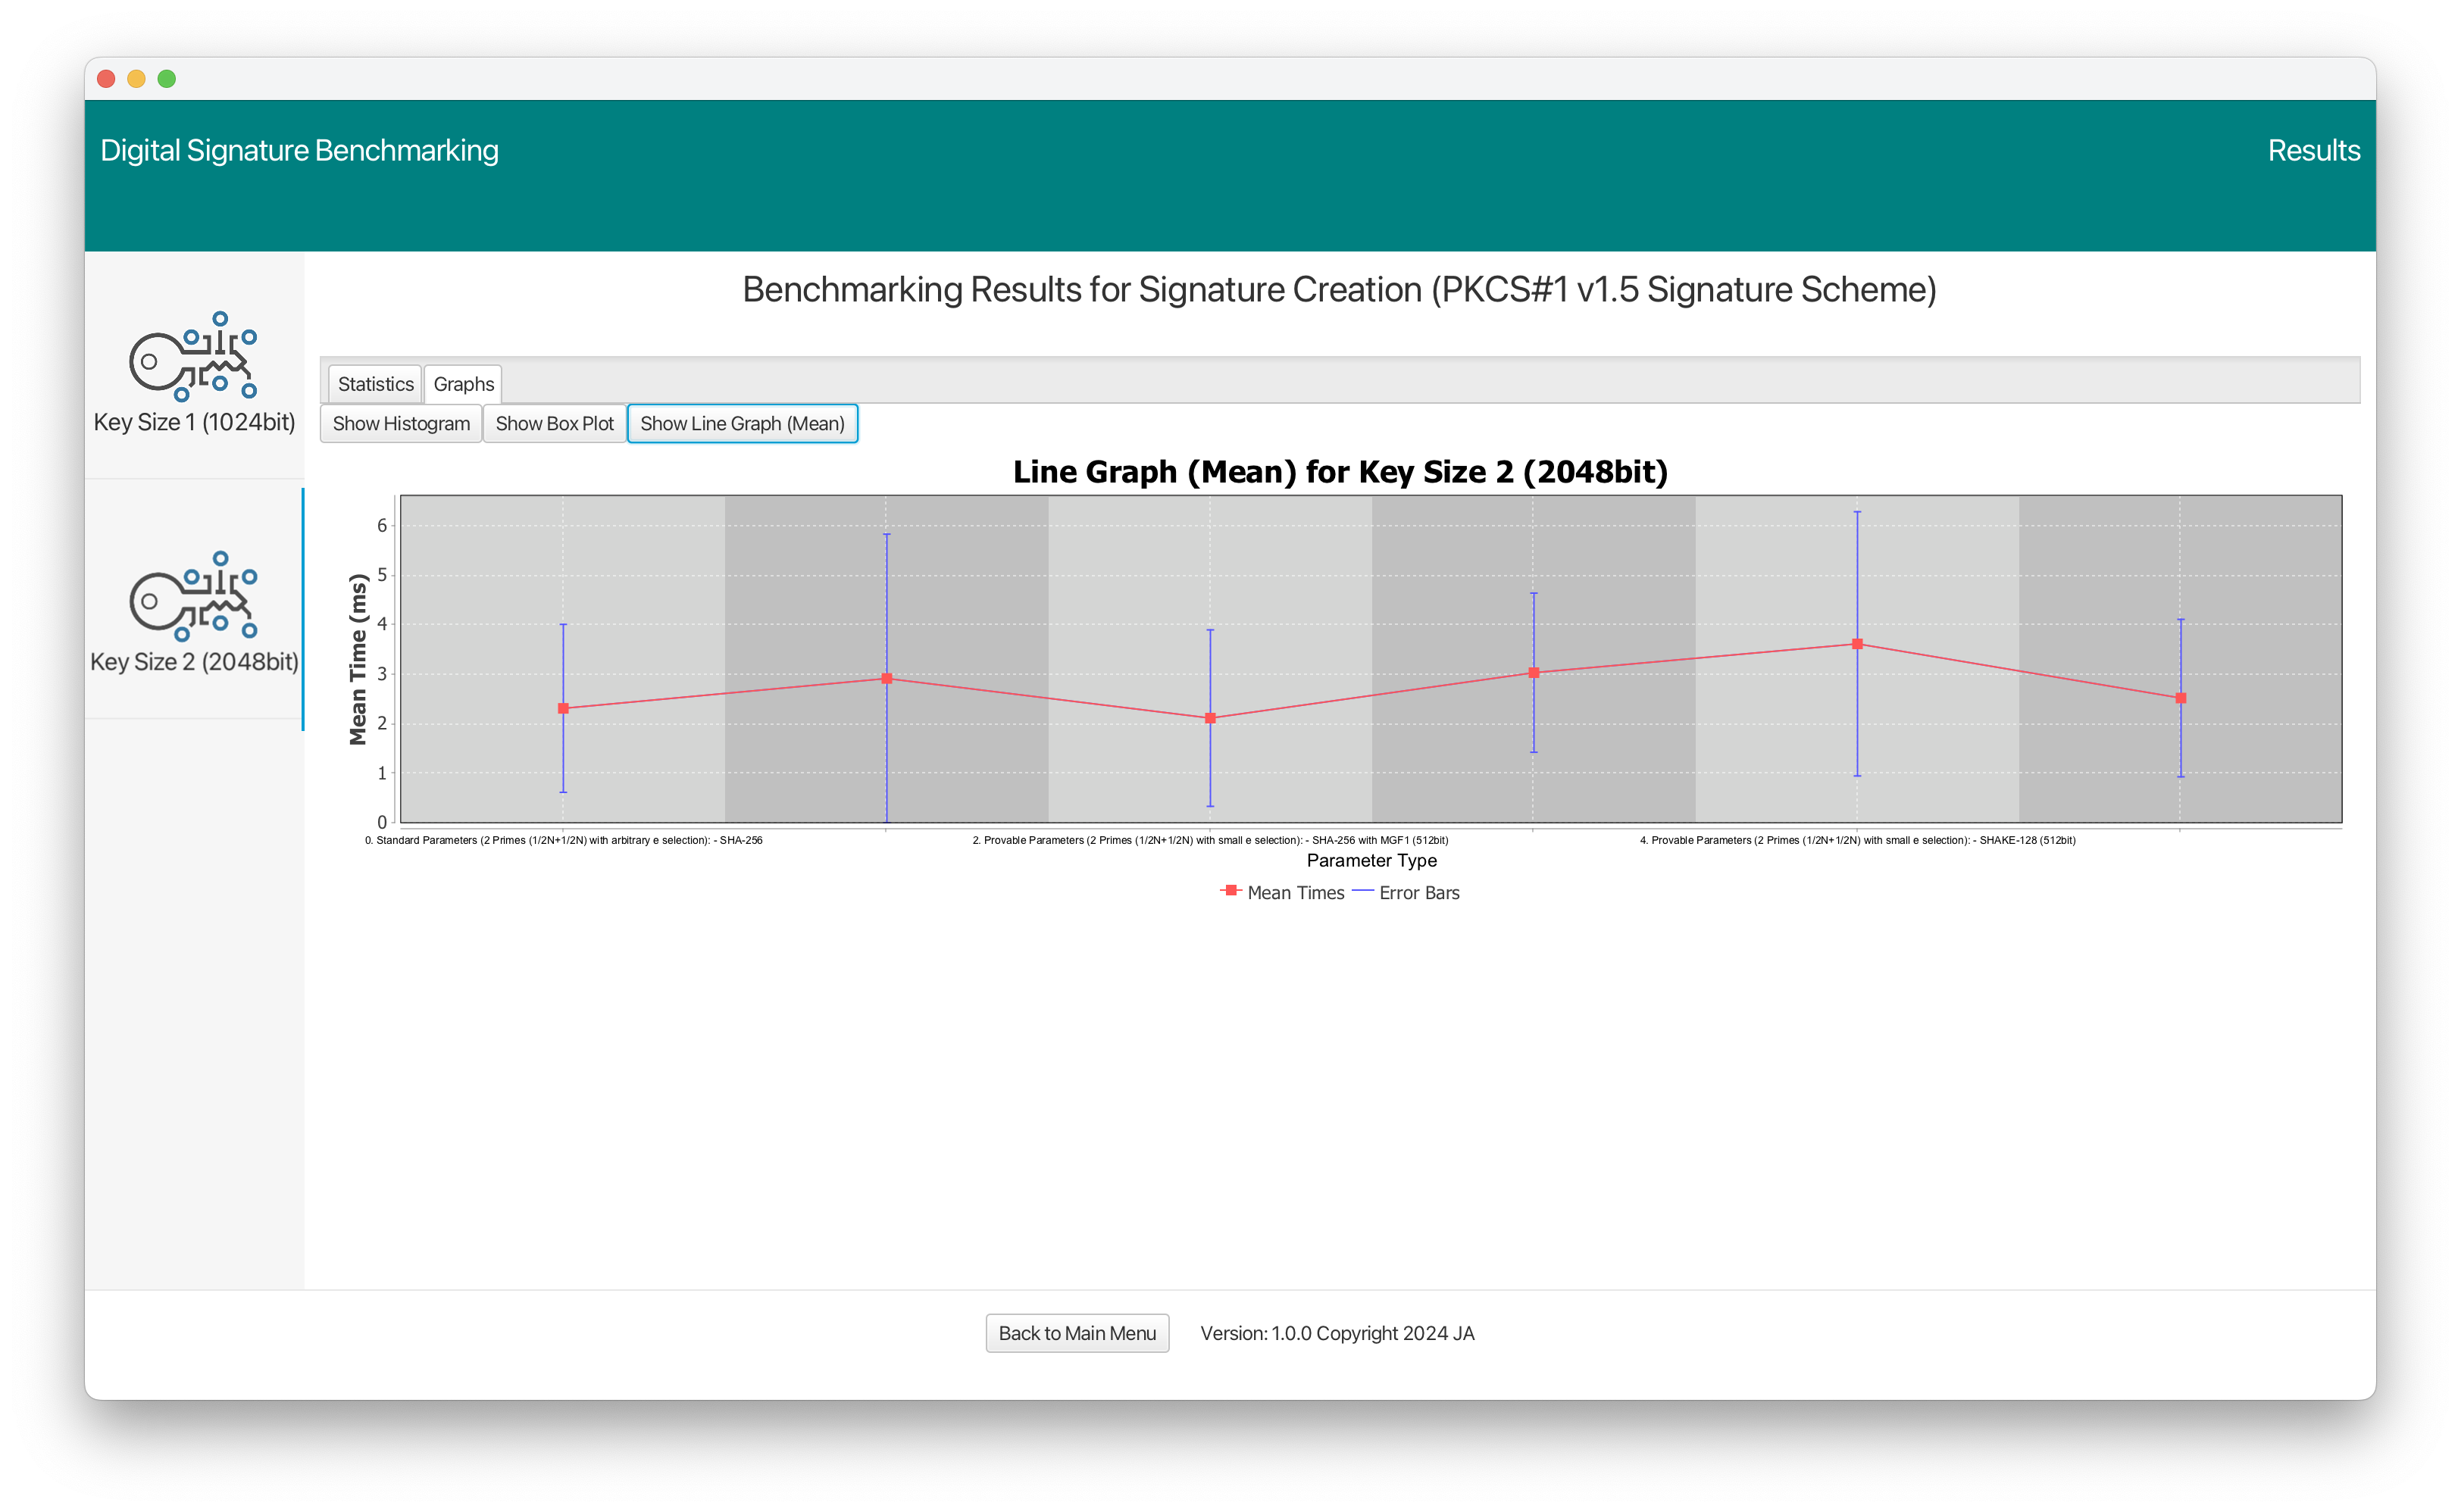
\includegraphics[width=\textwidth]{main_pictures/ui/signing/signing10-2.png}} % Adding border here
        \caption{Comparison Benchmarking: Signature Generation: Overlaid Line graph for mean times}
        \label{fig:image2}
    \end{minipage}
\end{figure}

Signature generation results can also be visualised graphically, accessible under the "Graphs" tab in the central pane. These graphs, which correlate to key configuration-hash function combinations from the results table, offer an alternate method for interpreting the results.

\begin{comment}
Another way to interpret signature generation results is visually through graphical representation and this aligns with key configurations from the respective results table. The alternative view can be found under the "Graphs" tab, located in the central tab pane where the results table is placed. Accessing and interpreting these graphs follows the same procedure as those created during the benchmarking of key generation. 
\end{comment}
\subsection{Comparison Benchmarking: Signature Verification}

\begin{figure}[H]
    \centering
    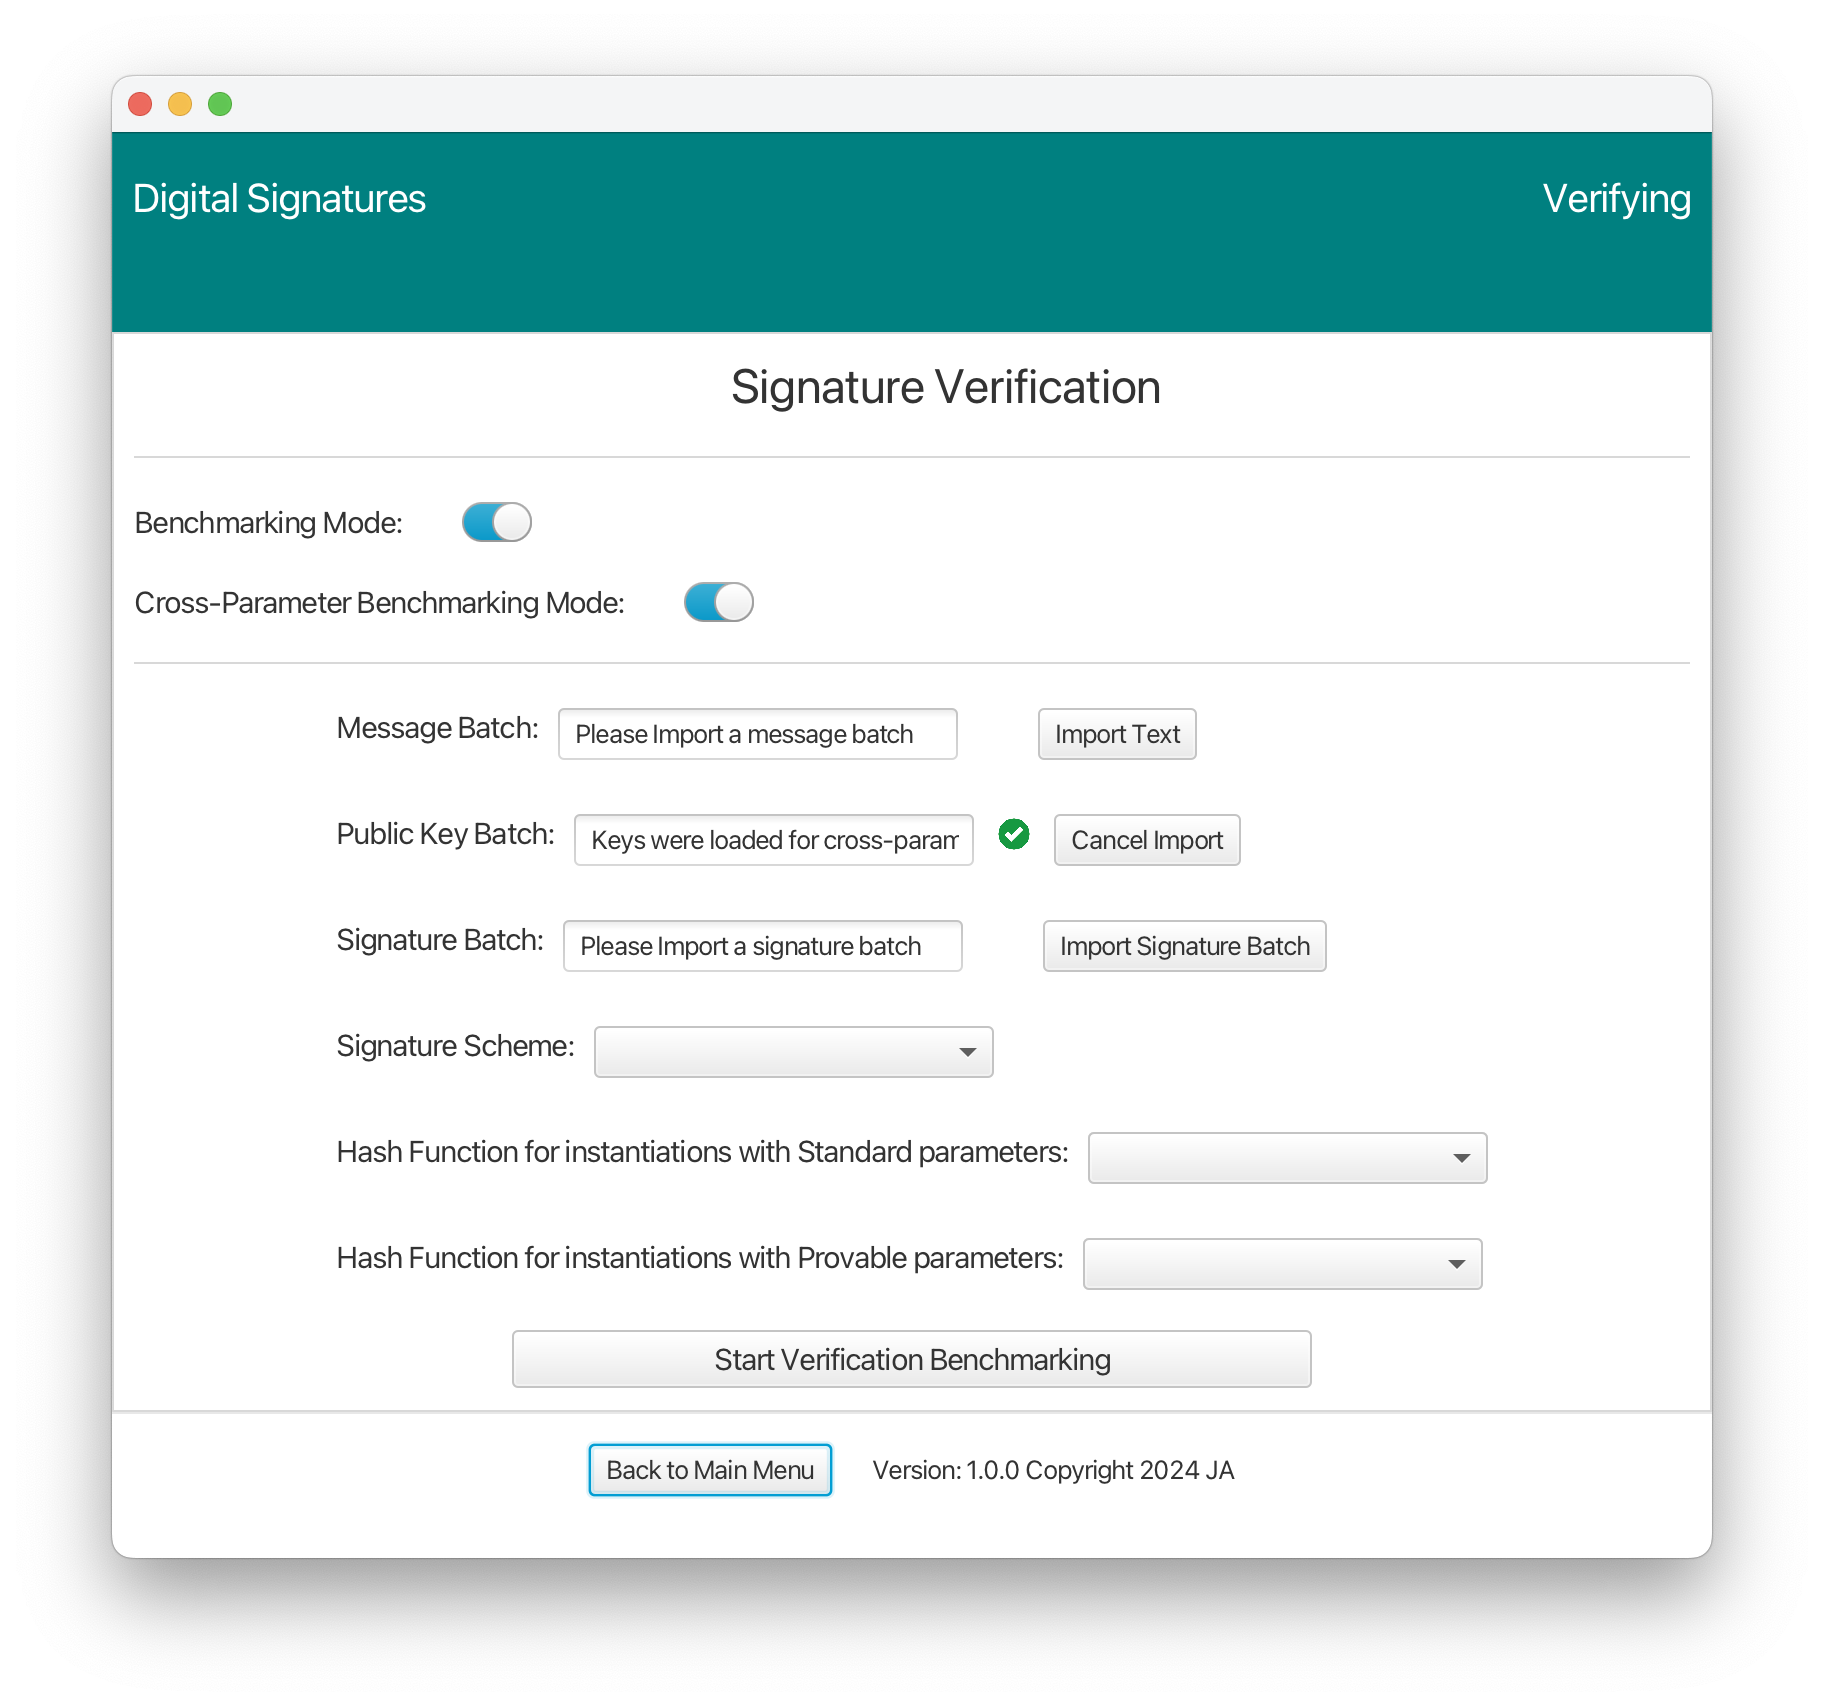
\includegraphics[scale= 0.4]{main_pictures/ui/verifying/verifying0.png}
    \caption{Comparison Benchmarking: Signature Verification}
\end{figure}

Similar to the process for signature generation, the signature verification screen for comparison benchmarking is accessible after completing a key generation benchmark in comparison mode. This procedure also includes preloading a batch of keys. However, the key distinction lies in the type of key batch loaded. In the case of signature verification, it's a public key batch that gets preloaded, as opposed to a private key batch used for signature generation.


\begin{figure}[H]
    \centering % Center the images
    
    % First image in a minipage
    \begin{minipage}{0.4\textwidth}
        \centering
        \fbox{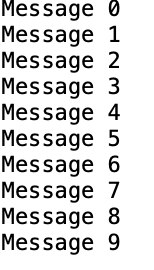
\includegraphics[width=0.4\textwidth]{main_pictures/ui/signing/signing2.png}} % Adding border here
        \caption{Signature Verification (Test message batch (testMessages.txt))}
        \label{fig:image1}
    \end{minipage}
    \hfill % Add some space between the images
    % Second image in a minipage
    \begin{minipage}{0.58\textwidth}
        \centering
        \fbox{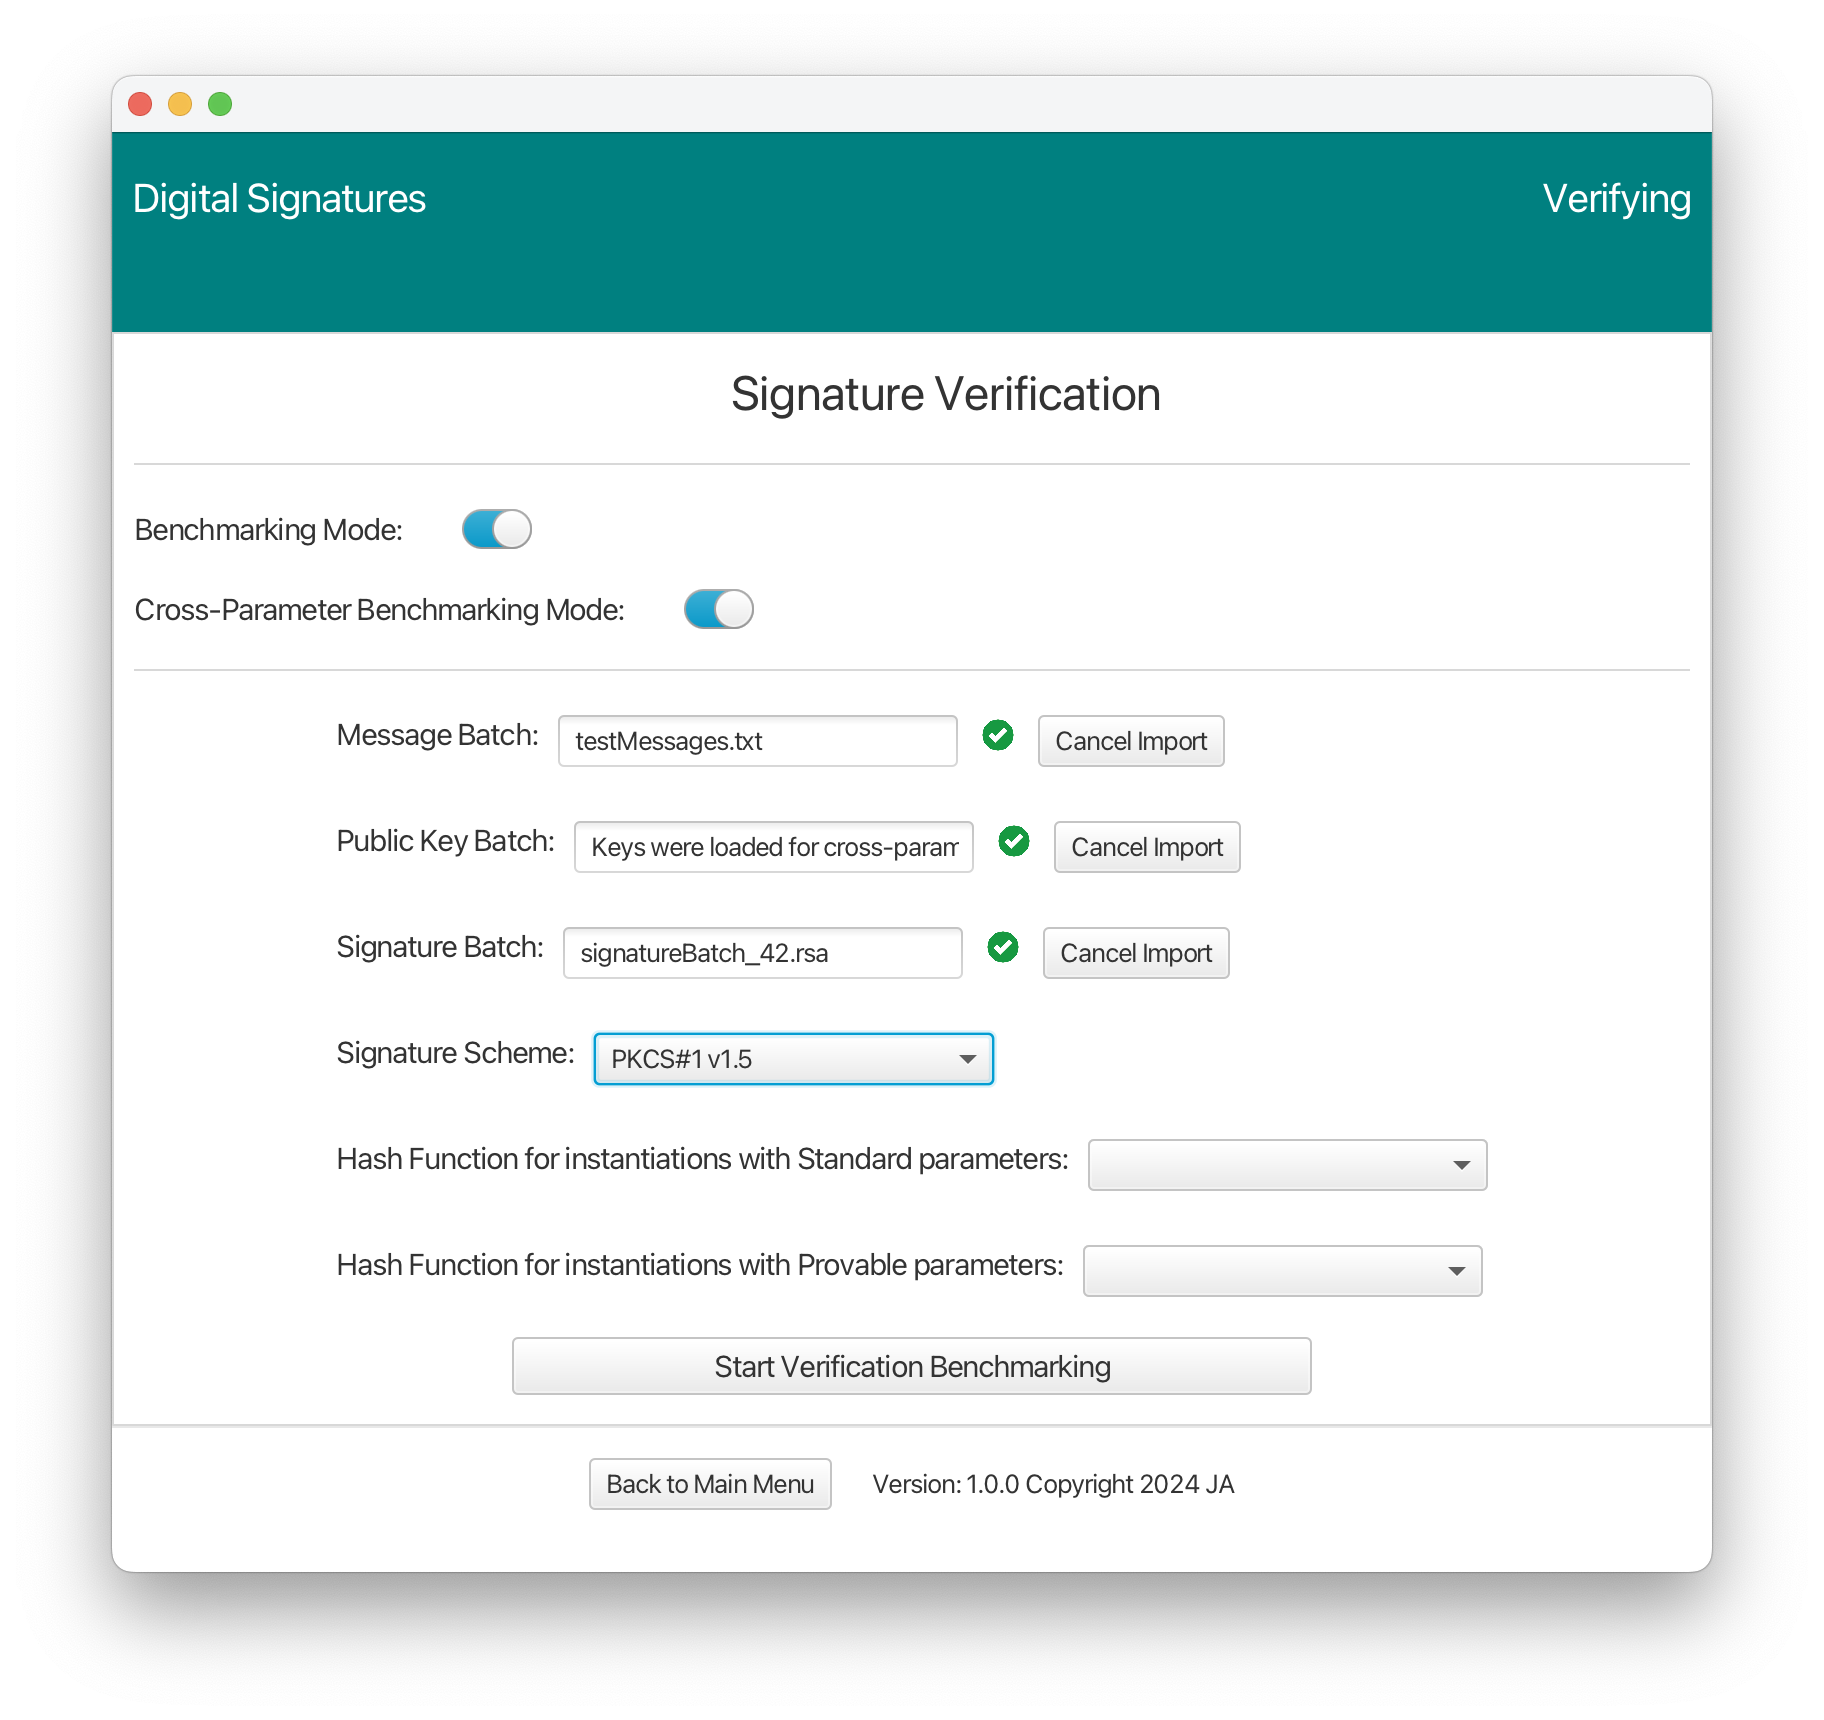
\includegraphics[width=\textwidth]{main_pictures/ui/verifying/verifying2.png}} % Adding border here
        \caption{Comparison Benchmarking: Signature Verification (Imported message batch)}
        \label{fig:image2}
    \end{minipage}
\end{figure}

Aside from the preloaded public key batch used for comparison benchmarking, the signature verification screen includes fields for importing both message and signature batches. For correctness, it's necessary that the submitted message batch aligns with the submitted signature batch. Moreover, these batches must be compatible with the public key batch, which, in turn, is associated with the private key batch employed during the prior signature generation phase.


\begin{figure}[H]
    \centering % Center the images
    
    % First image in a minipage
    \begin{minipage}{0.49\textwidth}
        \centering
        \fbox{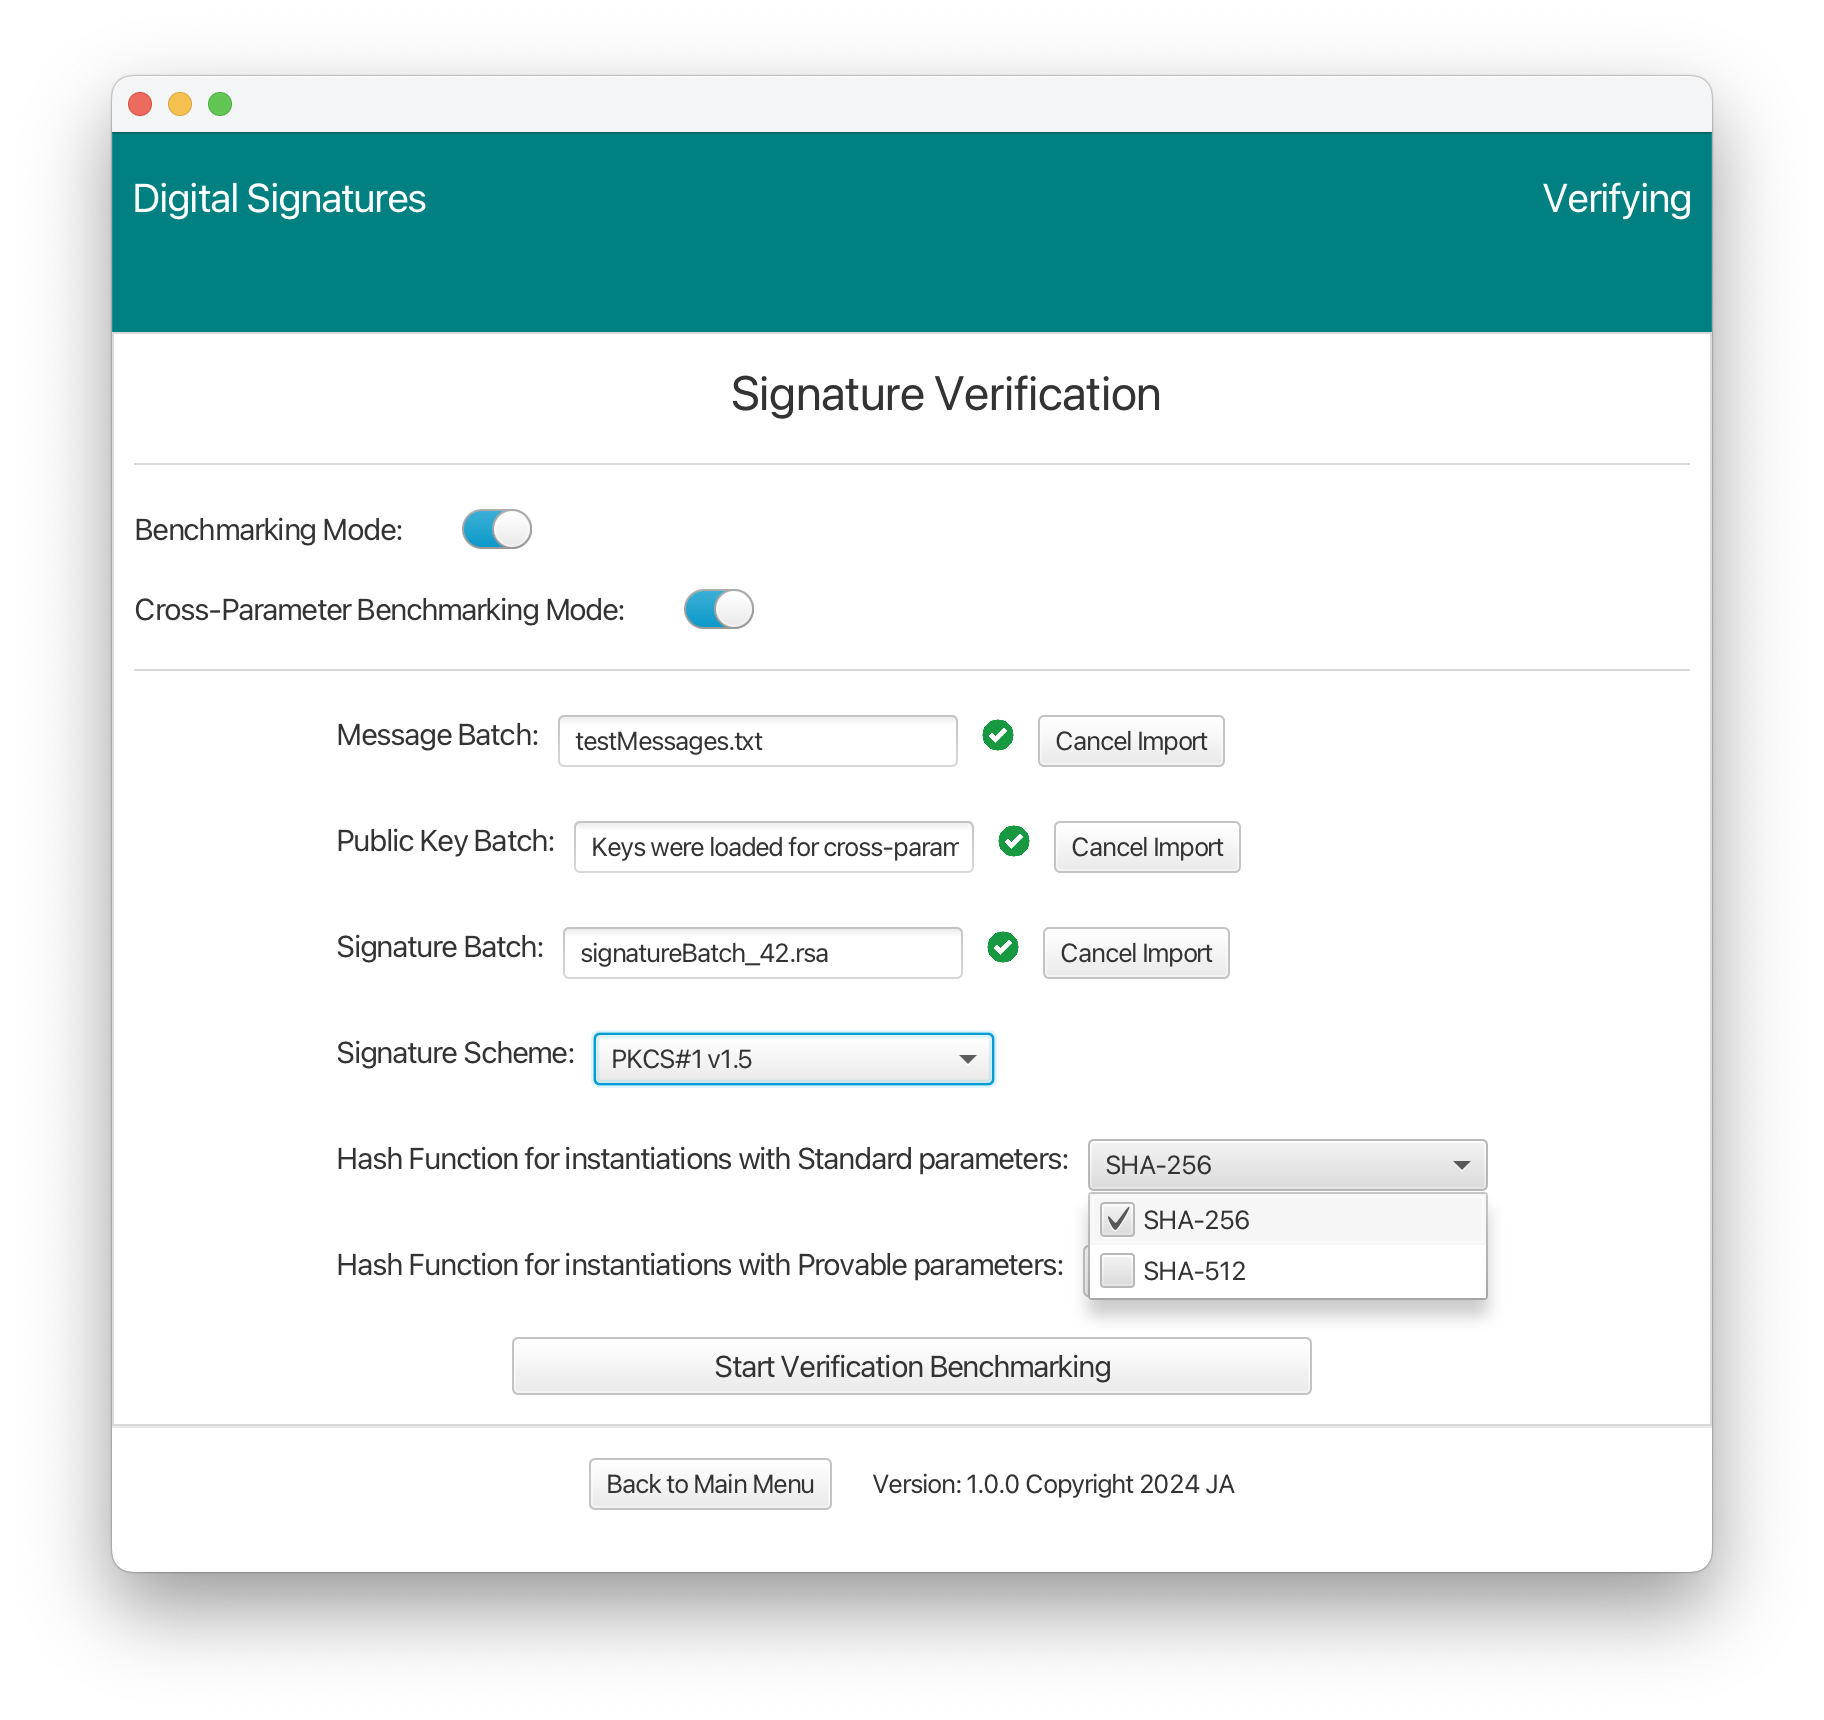
\includegraphics[width=\textwidth]{main_pictures/ui/verifying/verifying3.png}} % Adding border here
        \caption{Comparison Benchmarking: Signature Verification (Standard Parameter Hash Functions)}
        \label{fig:image1}
    \end{minipage}
    \hfill % Add some space between the images
    % Second image in a minipage
    \begin{minipage}{0.49\textwidth}
        \centering
        \fbox{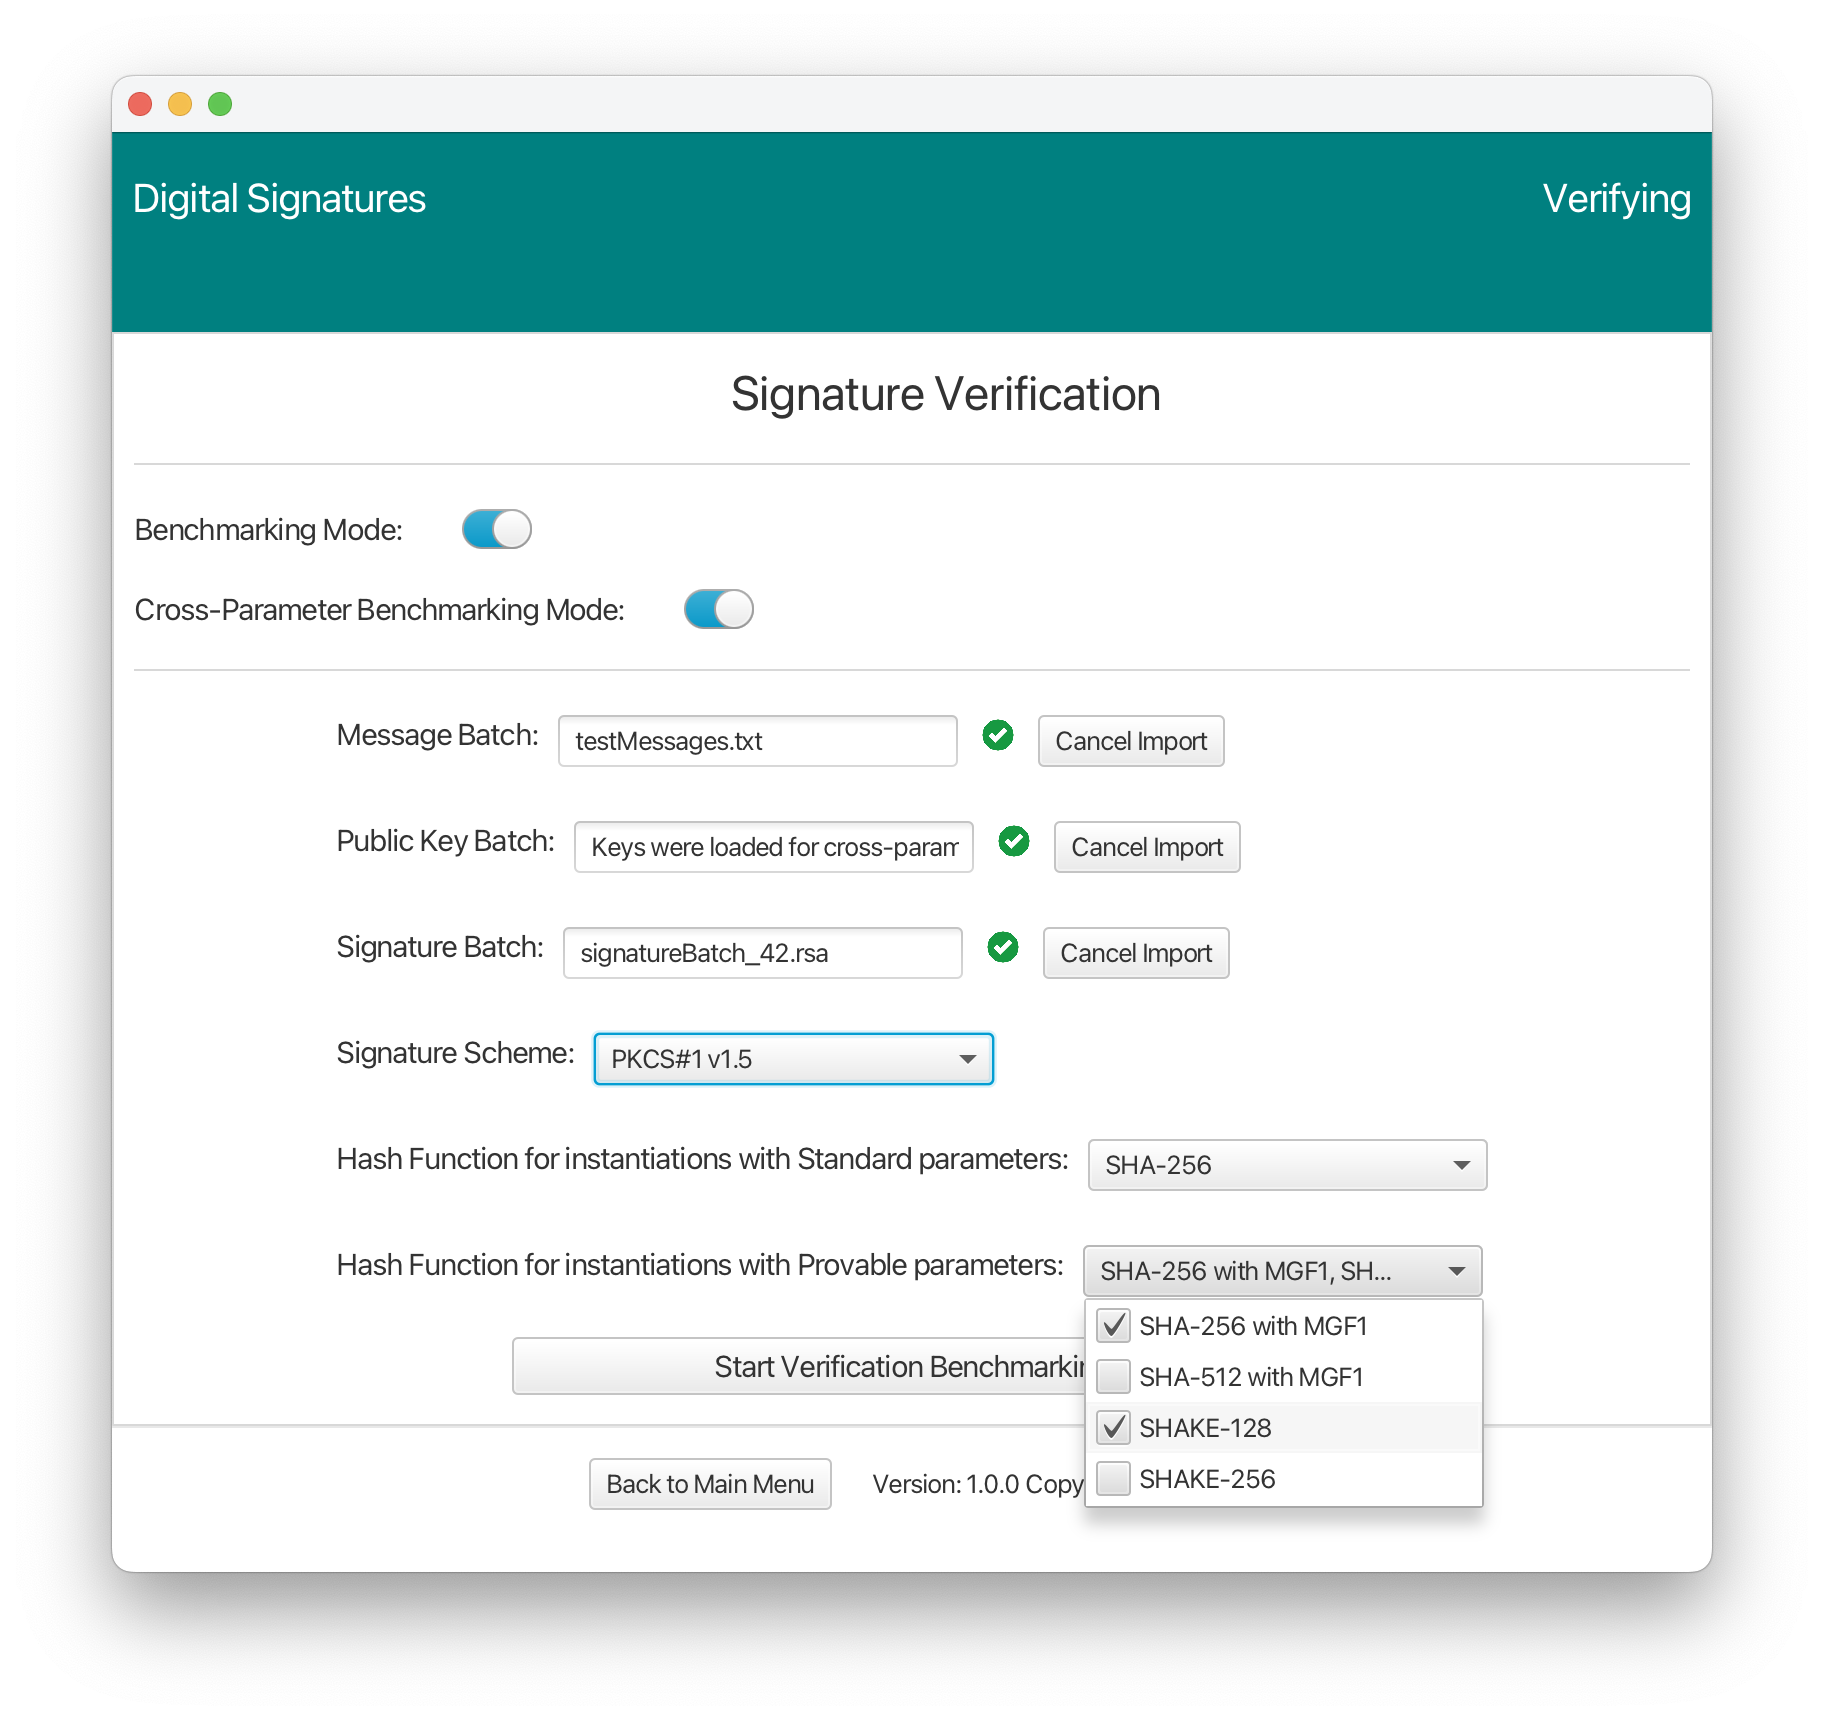
\includegraphics[width=\textwidth]{main_pictures/ui/verifying/verifying4.png}} % Adding border here
        \caption{Comparison Benchmarking: Signature Verification (Provably Secure Parameter Hash Functions)}
        \label{fig:image2}
    \end{minipage}
\end{figure}


In signature verification (comparison) benchmarking, hash function selection must align with those used in signature generation to ensure correctness. The process starts with the user choosing matching hash functions for each parameter type. This is vital because the hash functions used must correspond to the message-signature pairs created in the signature generation phase, which used the private key batch related to the currently imported public key batch.

Upon selecting "Start Verification Benchmarking," the SignatureController validates the number of signatures against the message batch and chosen hash functions. If there's a mismatch, an alert notifies the user of the discrepancy. Following successful validation, the SignatureModel takes over to execute the verification benchmarking. This involves comparing the signature batch with the message batch and public keys, using the selected signature scheme and hash functions. The process generates batches of verification results for each entered key size, and a progress bar provides real-time progress updates.


\begin{comment}
Hash function selection for signature verification in comparison benchmarking mode mirrors the mechanism used for signature creation. For correctness,  the selected hash functions for each parameter type must match those submitted for the equivalent message-signature batch pairing generated during the prior signature generation process that contained the private key batch  corresponding to the currently imported public key batch.

Upon selection of the "Start Verification Benchmarking" button, a chain of validation and execution steps are executed. The SignatureController first verifies that the number of signatures in the signature batch matches the expected based on the number of messages and selected hash function choices. Should a discrepancy arise during this stage with a mismatch between the number of signatures and message batch/hash function combination, the interface promptly presents an alert, informing the user of the necessary corrective measures.

Once the preliminary checks are met, the SignatureModel assumes control to execute the benchmarking task for verification. It compares the provided signature batch against the message batch with the public key batch using the selected signature scheme and relevant hash function to key combinations. A byproduct of the process is the generation of batches of verification results corresponding to each previously entered key size, while a progress bar is displayed for a length of time spanning the duration of the task allowing for real-time indication of progress.
\end{comment}



\newpage
%TC:ignore
\textbf{Comparison Benchmarking: Signature Verification Results Screen}
%TC:endignore

\begin{figure}[H]
    \centering
    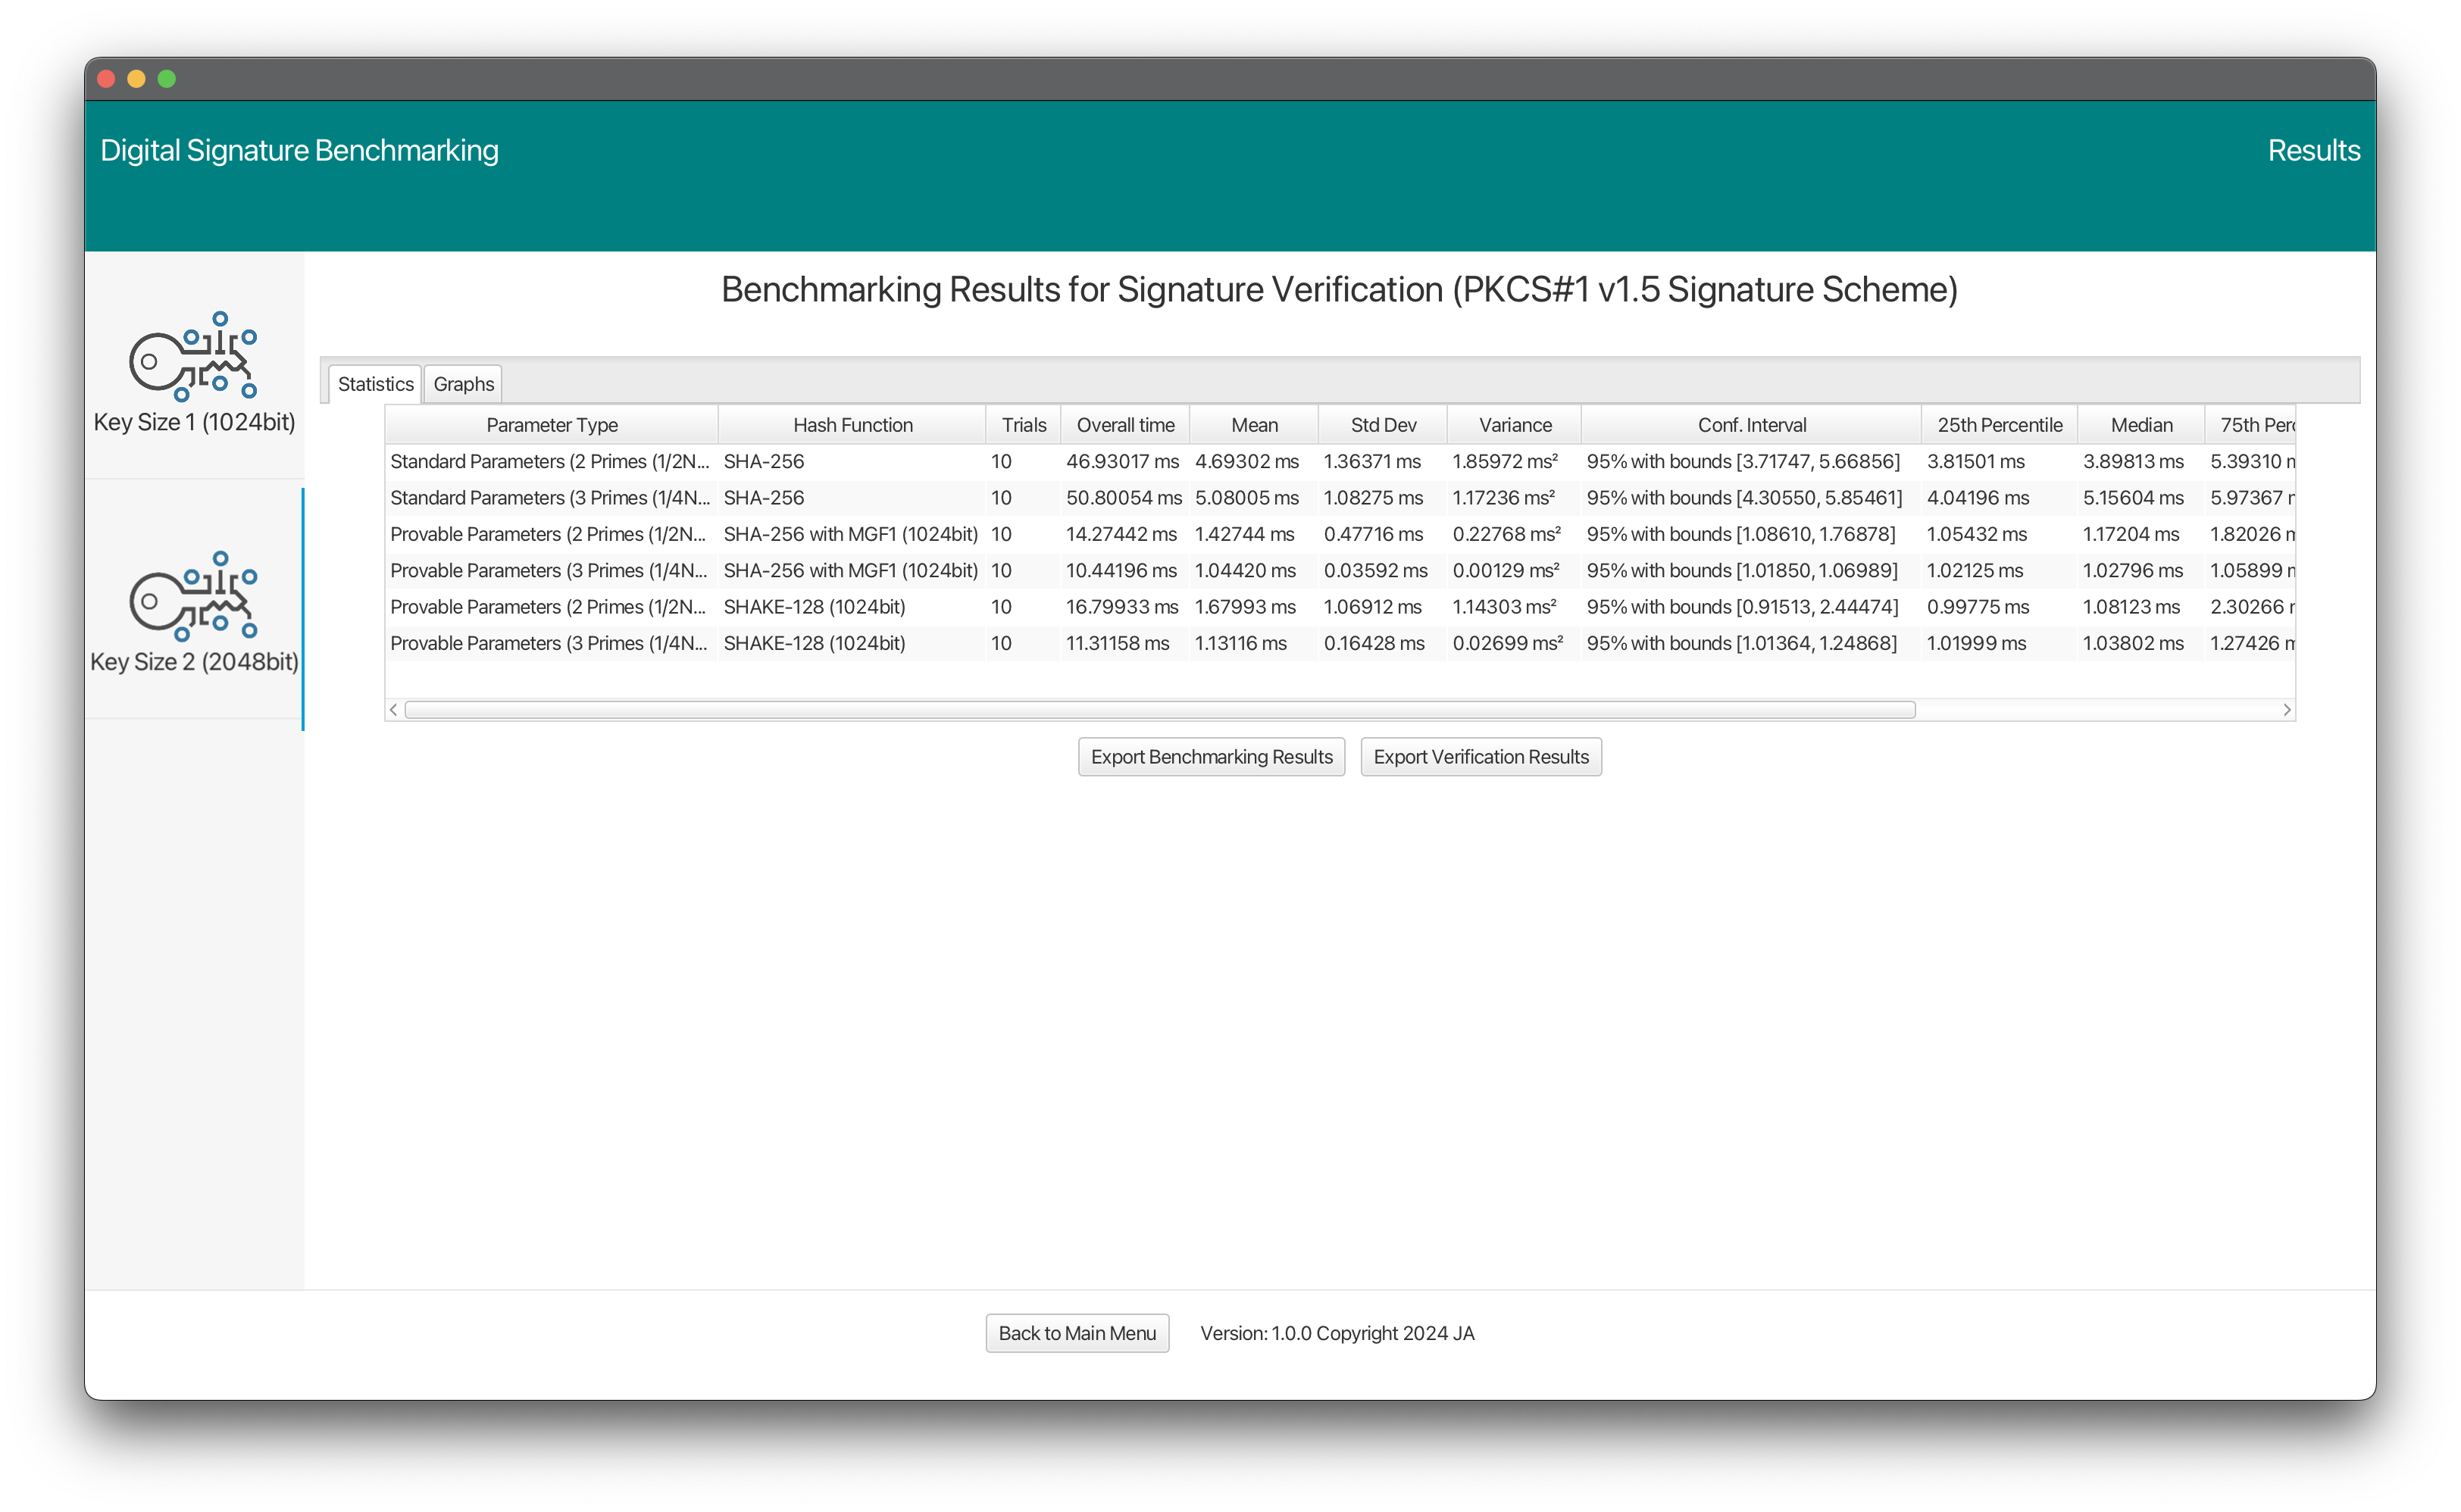
\includegraphics[scale= 0.325]{main_pictures/ui/verifying/verifying6.png}
    \caption{Comparison Benchmarking: Signature Verification (Results Screen)}
\end{figure}

Once the signature verification benchmarking concludes, the ResultsController takes over to showcase the obtained results. The layout of this results screen is largely as was shown for signature generation. The distinction is the enabling of the export of verification results for each key size displayed below each results table.

\begin{figure}[H]
    \centering % Center the images
    
    % First image in a minipage
    \begin{minipage}{0.7\textwidth}
        \centering
        \fbox{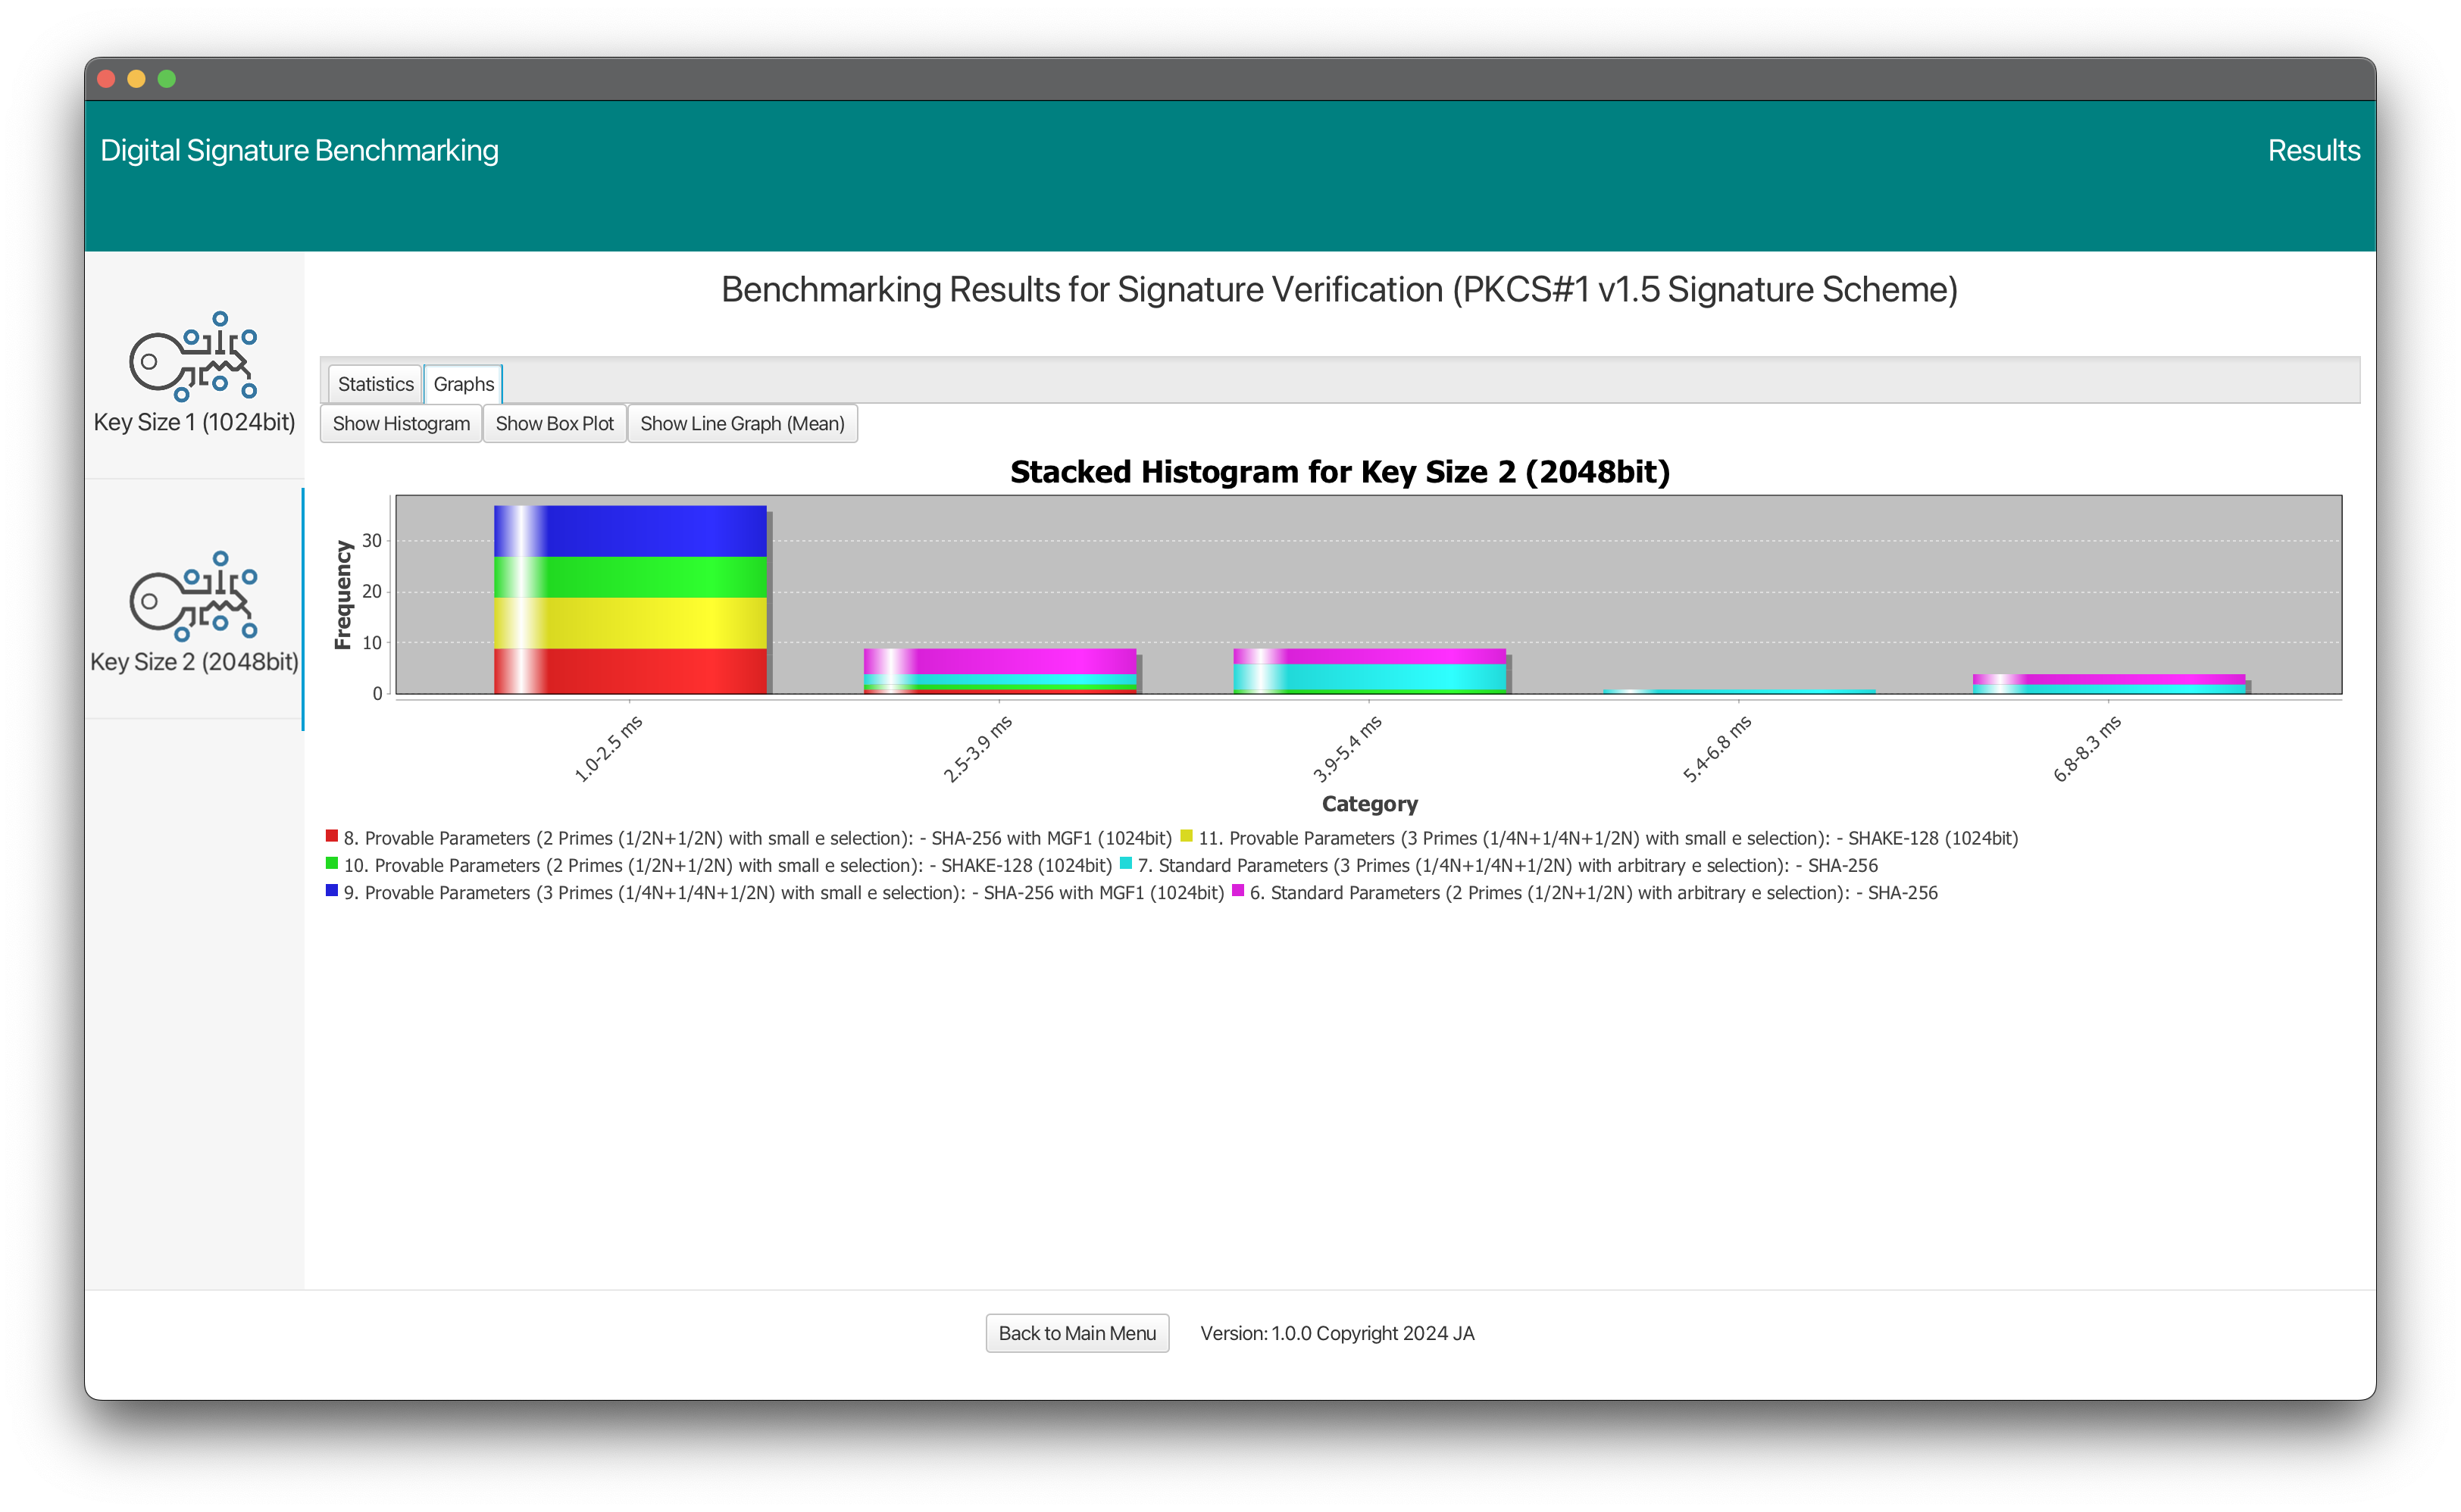
\includegraphics[width=\textwidth]{main_pictures/ui/verifying/verifying7.png}} % Adding border here
        \caption{Comparison Benchmarking: Signature Verification: Overlaid Histogram}
        \label{fig:image1}
    \end{minipage}
    \hfill % Add some space between the images
    % Second image in a minipage
    \begin{minipage}{0.7\textwidth}
        \centering
        \fbox{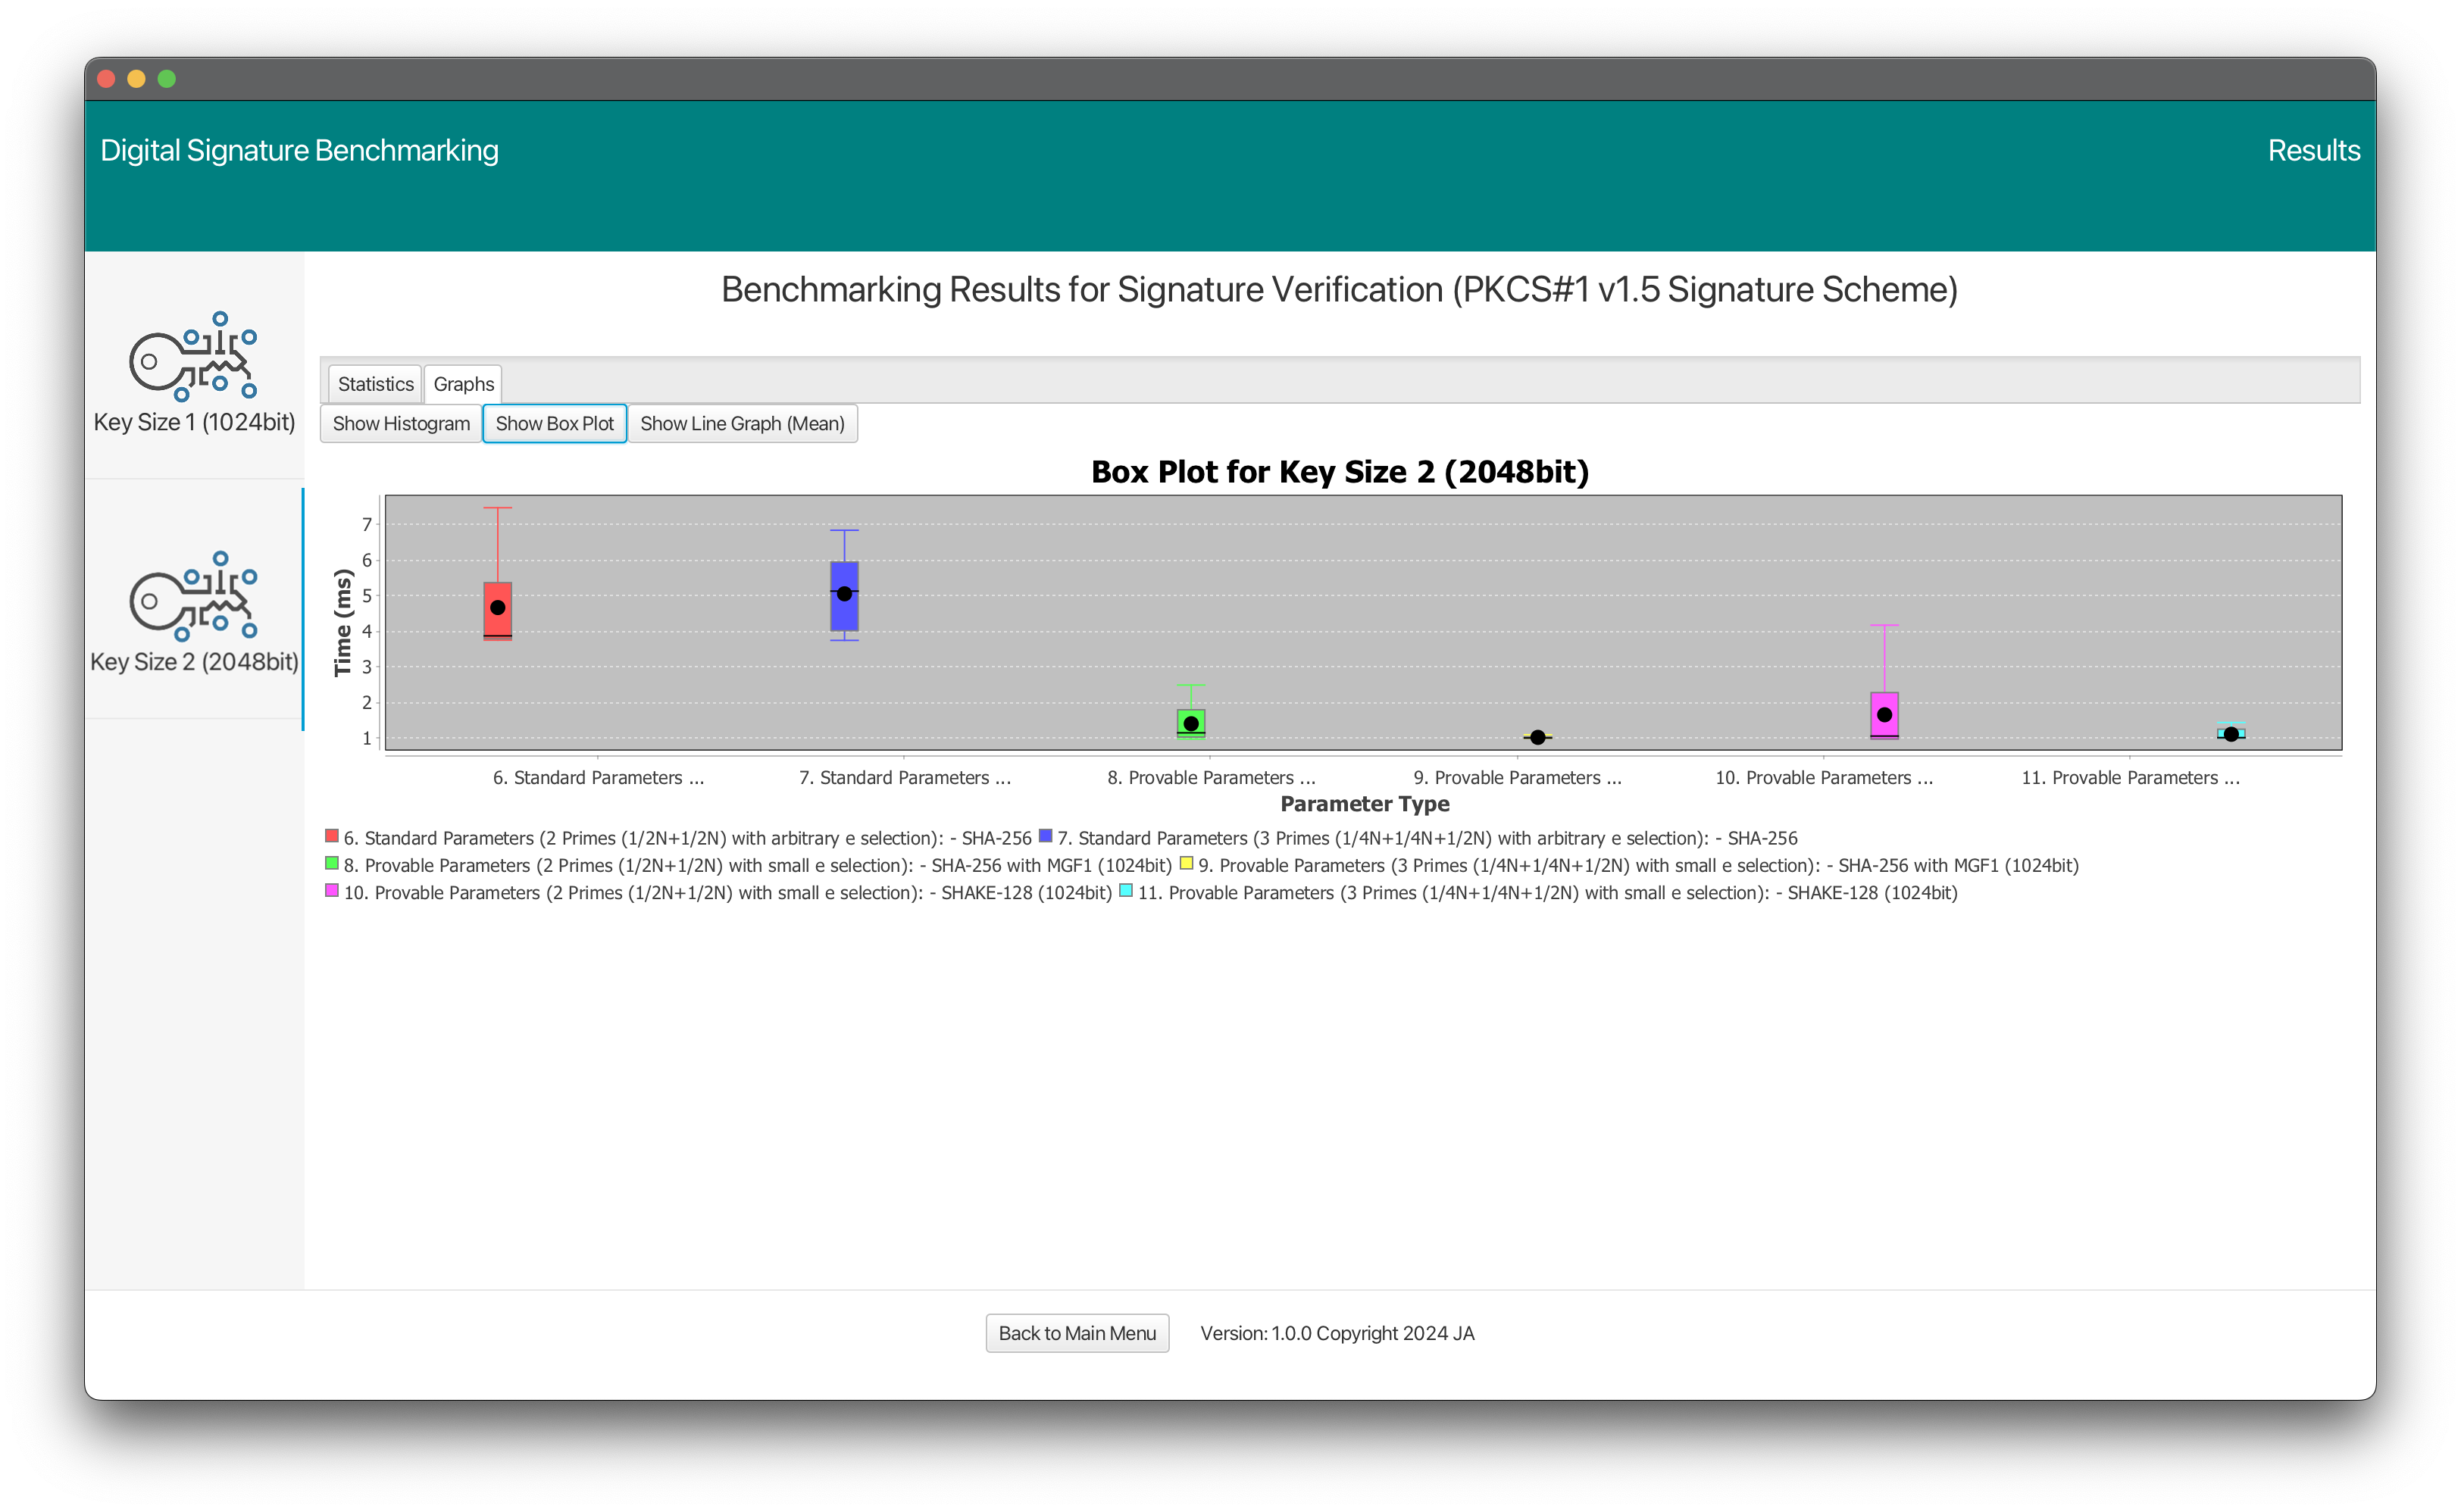
\includegraphics[width=\textwidth]{main_pictures/ui/verifying/verifying8.png}} % Adding border here
        \caption{Comparison Benchmarking: Signature Verification: Overlaid Box plot graph}
        \label{fig:image2} 
    \end{minipage}
     \begin{minipage}{0.7\textwidth}
        \centering
        \fbox{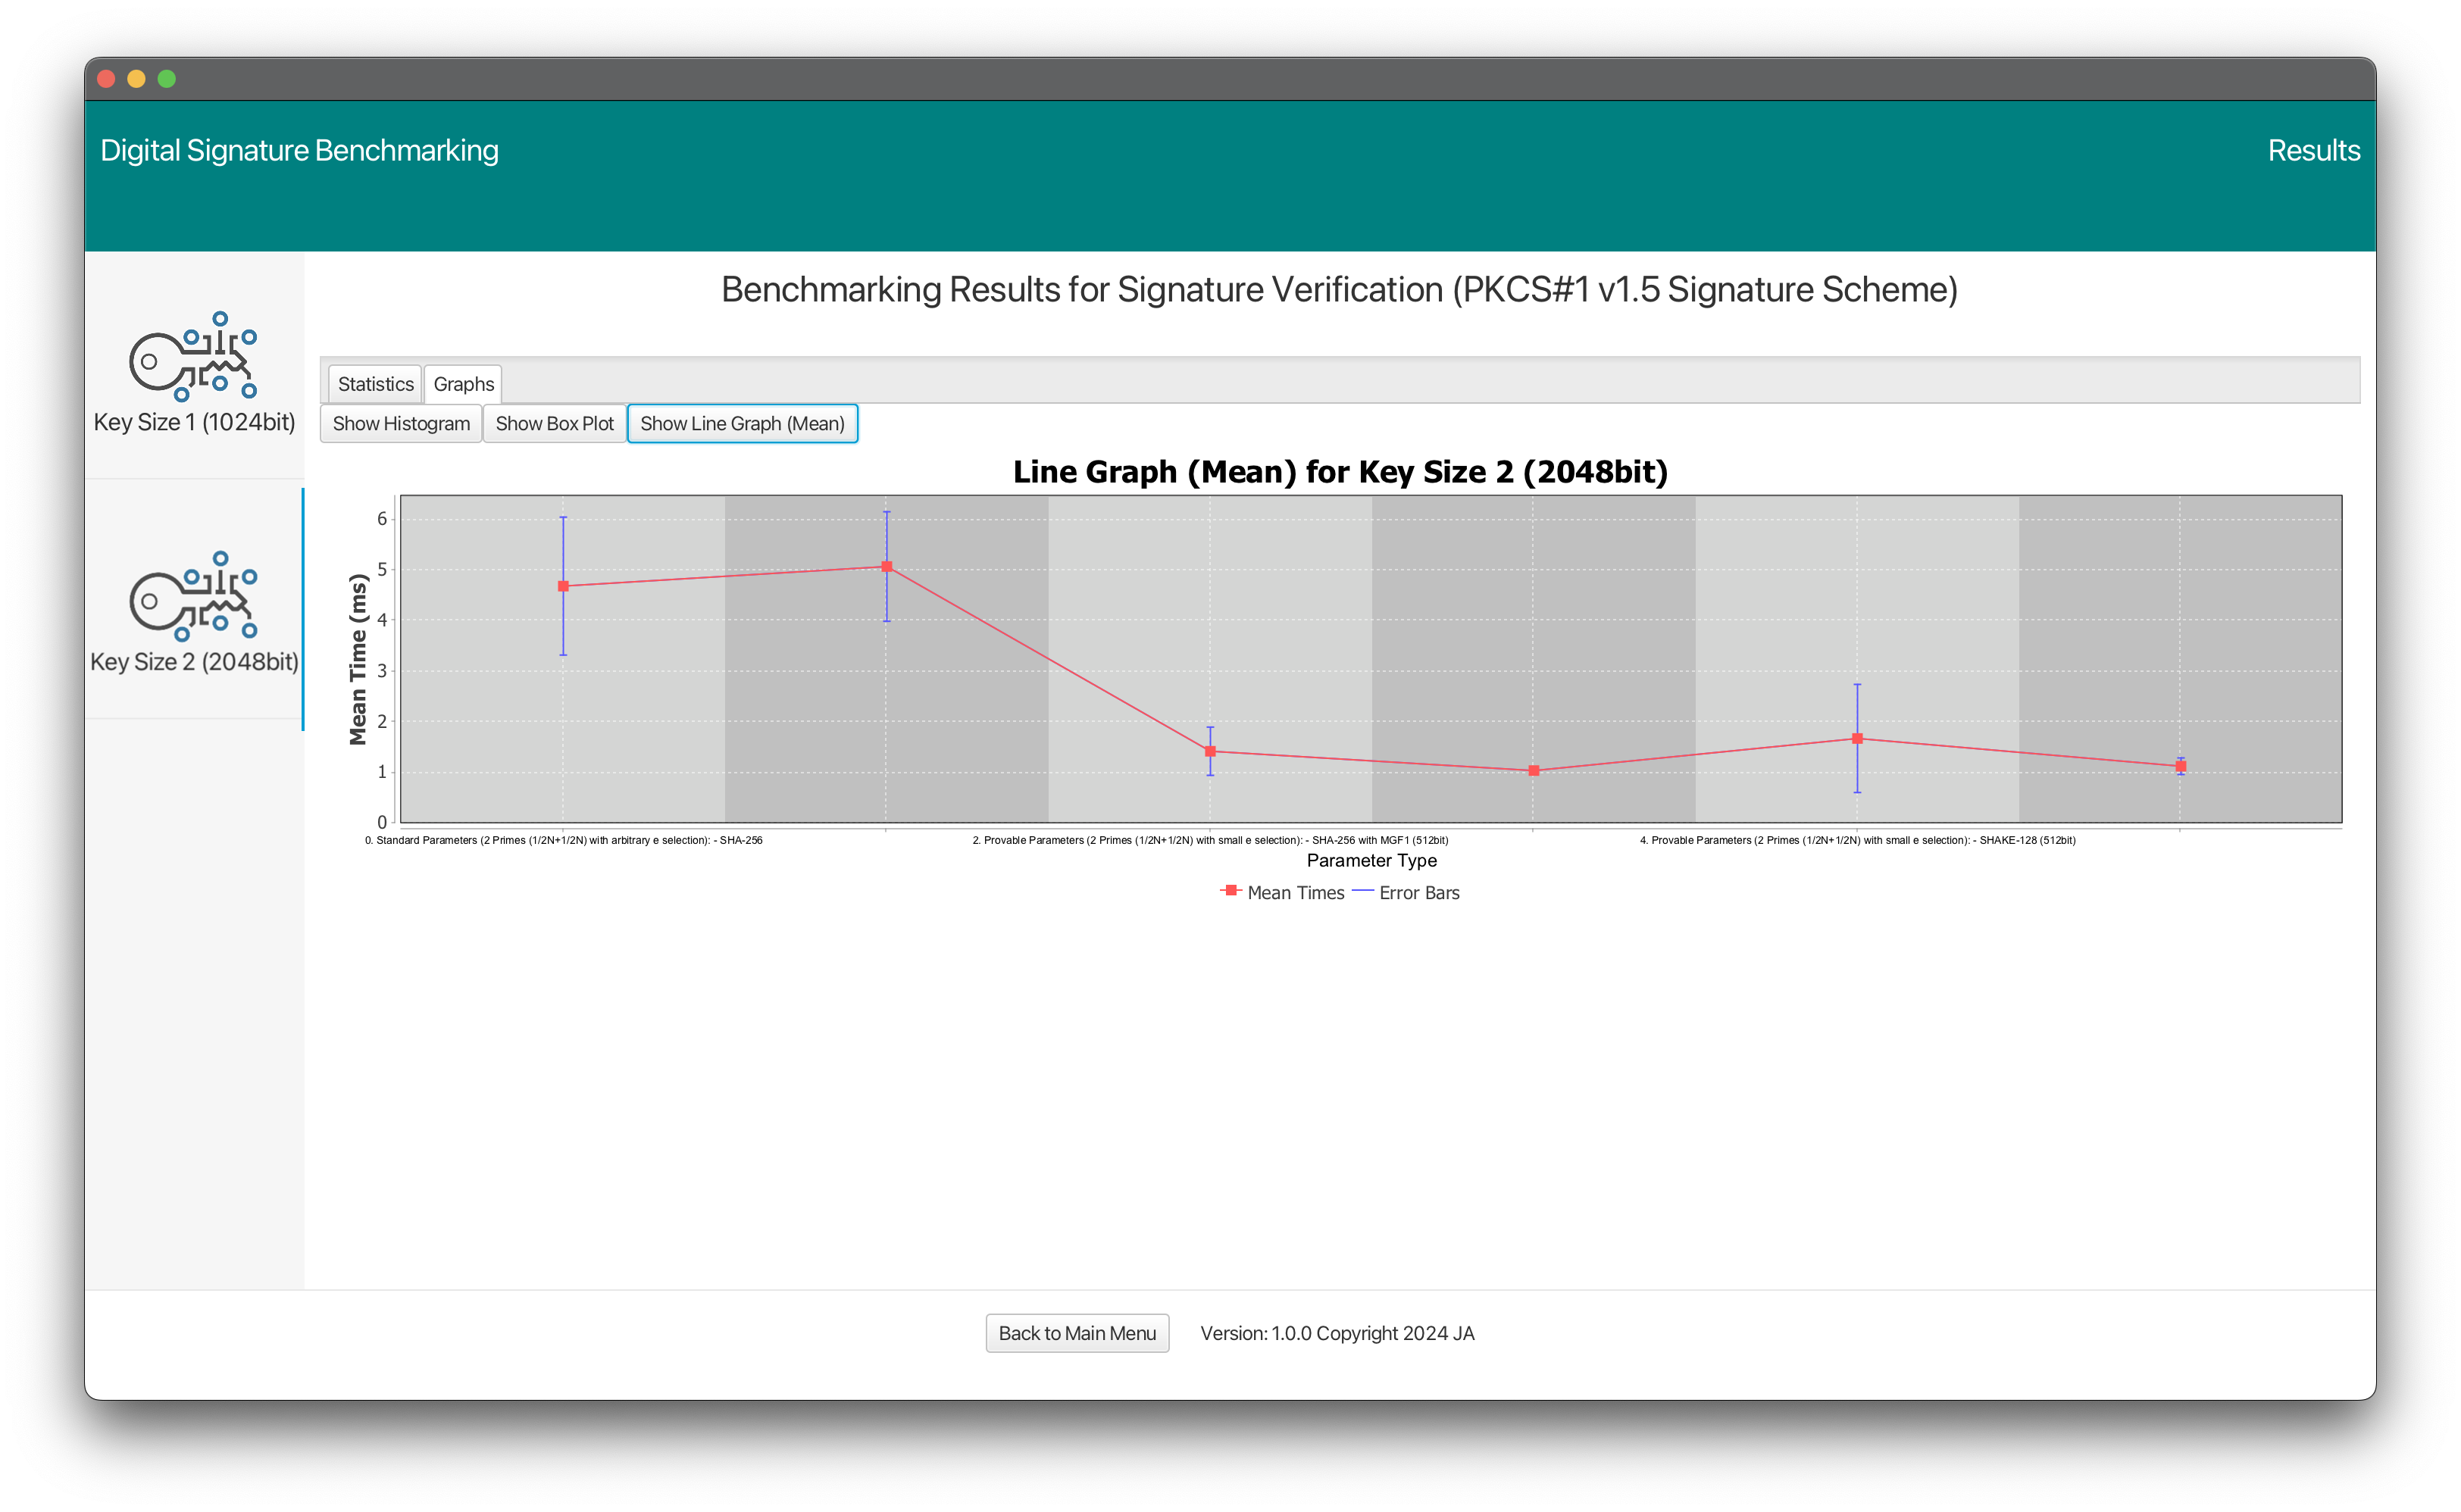
\includegraphics[width=\textwidth]{main_pictures/ui/verifying/verifying9.png}} % Adding border here
        \caption{Comparison Benchmarking: Signature Verification: Overlaid Line graph for mean times}
        \label{fig:image2}
    \end{minipage}
\end{figure}

\subsection{Comparison Benchmarking: Signature Processing for Message Recovery Schemes}

In the Signature processes, when utilising the message recovery ISO/IEC 9796-2 Scheme, there is a specific approach for handling non-recoverable portion when signature generation is performed and recovered portion of messages when signature verification is performed.

\begin{figure}[H]
    \centering % Center the images
    
    % First image in a minipage
    \begin{minipage}{0.2\textwidth}
        \centering
        \fbox{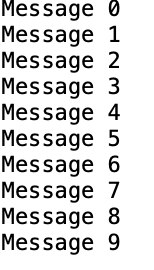
\includegraphics[width=\textwidth]{main_pictures/ui/signing/signing2.png}} % Adding border here
        \caption{Signature Creation (Test message batch (testMessages.txt))}

        \label{fig:image1}
    \end{minipage}
    \hfill % Add some space between the images
    % Second image in a minipage
    \begin{minipage}{0.7\textwidth}
        \centering
         \fbox{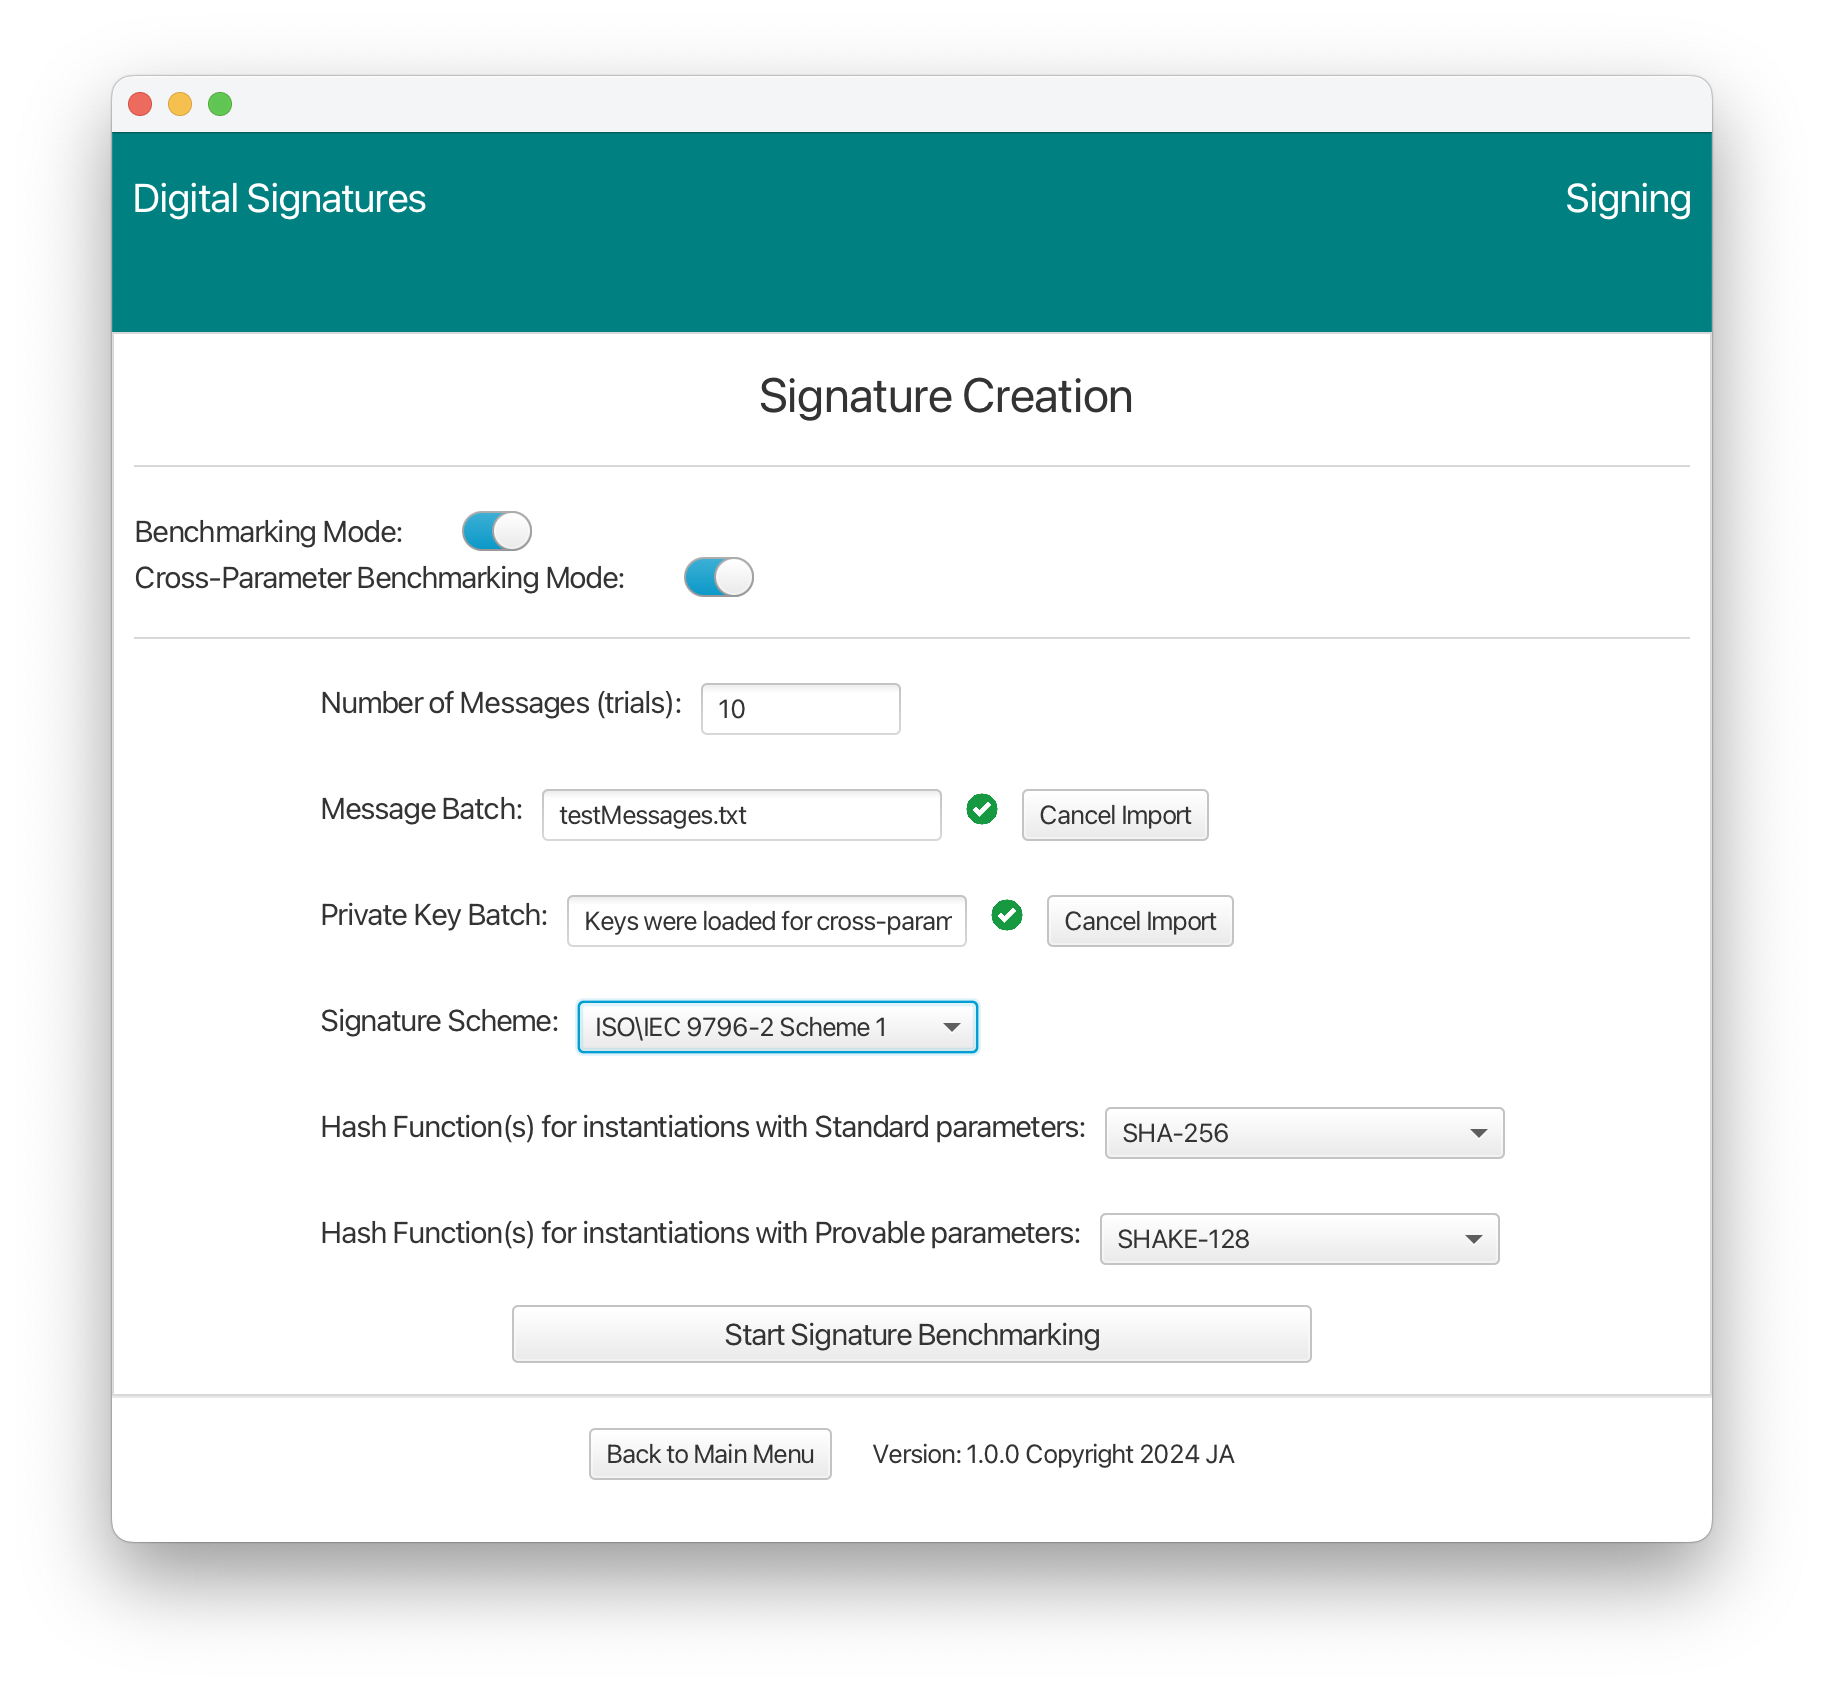
\includegraphics[width=\textwidth]{main_pictures/ui/signing/signing11.png}} % Adding border here
        \caption{Comparison Benchmarking: Signature Generation with ISO scheme selected}        \label{fig:image2}
    \end{minipage}
    
      \begin{minipage}{0.7\textwidth}
        \centering
         \fbox{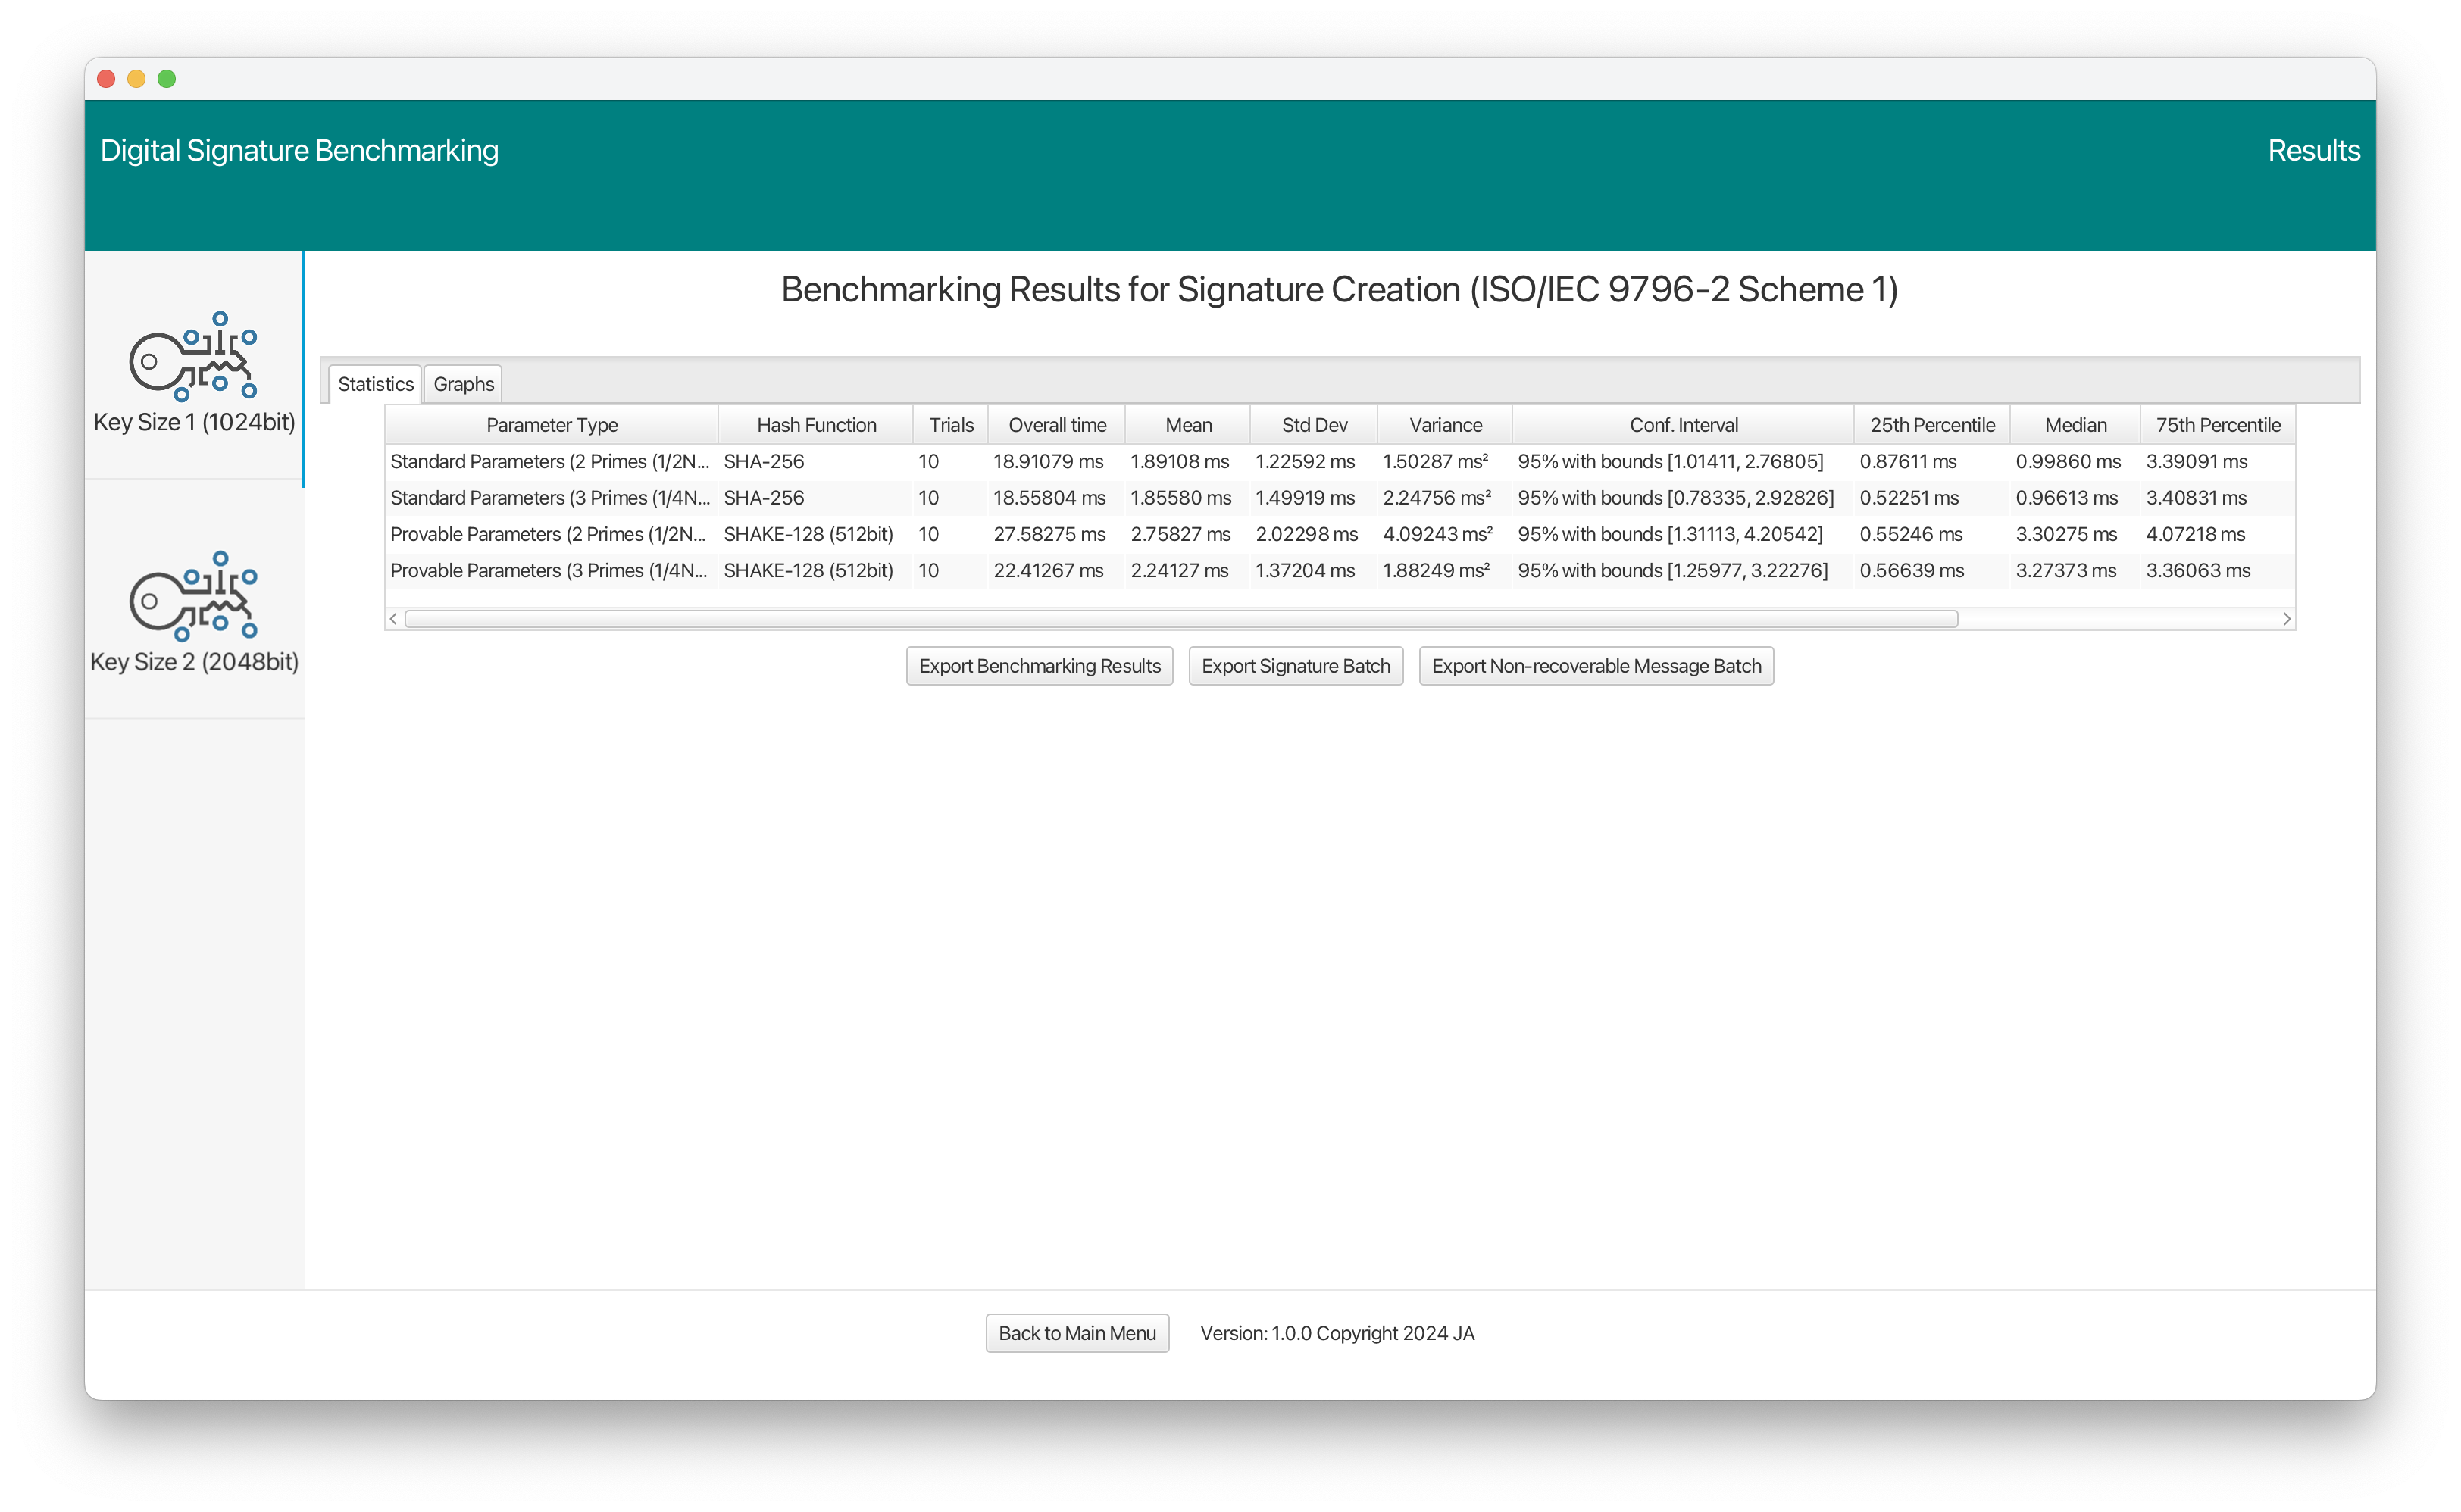
\includegraphics[width=\textwidth]{main_pictures/ui/signing/signing12.png}} % Adding border here
        \caption{Comparison Benchmarking: Signature Generation Results Screen (with Message Recovery Options)}        \label{fig:image2}
    \end{minipage}
\end{figure}

For signature generation this process involves exporting a batch of non-recoverable messages where each line corresponds with a signature. Lines are prefixed with a "1" to indicate the presence of a non-recoverable message and "0" when there is none. In this specific case, since all messages are too short to produce a non-recoverable part regardless of the key sizes selected, the resulting file comprises a sequence of "0" flags, each separated by a new line.


\begin{figure}[H]
    \centering
    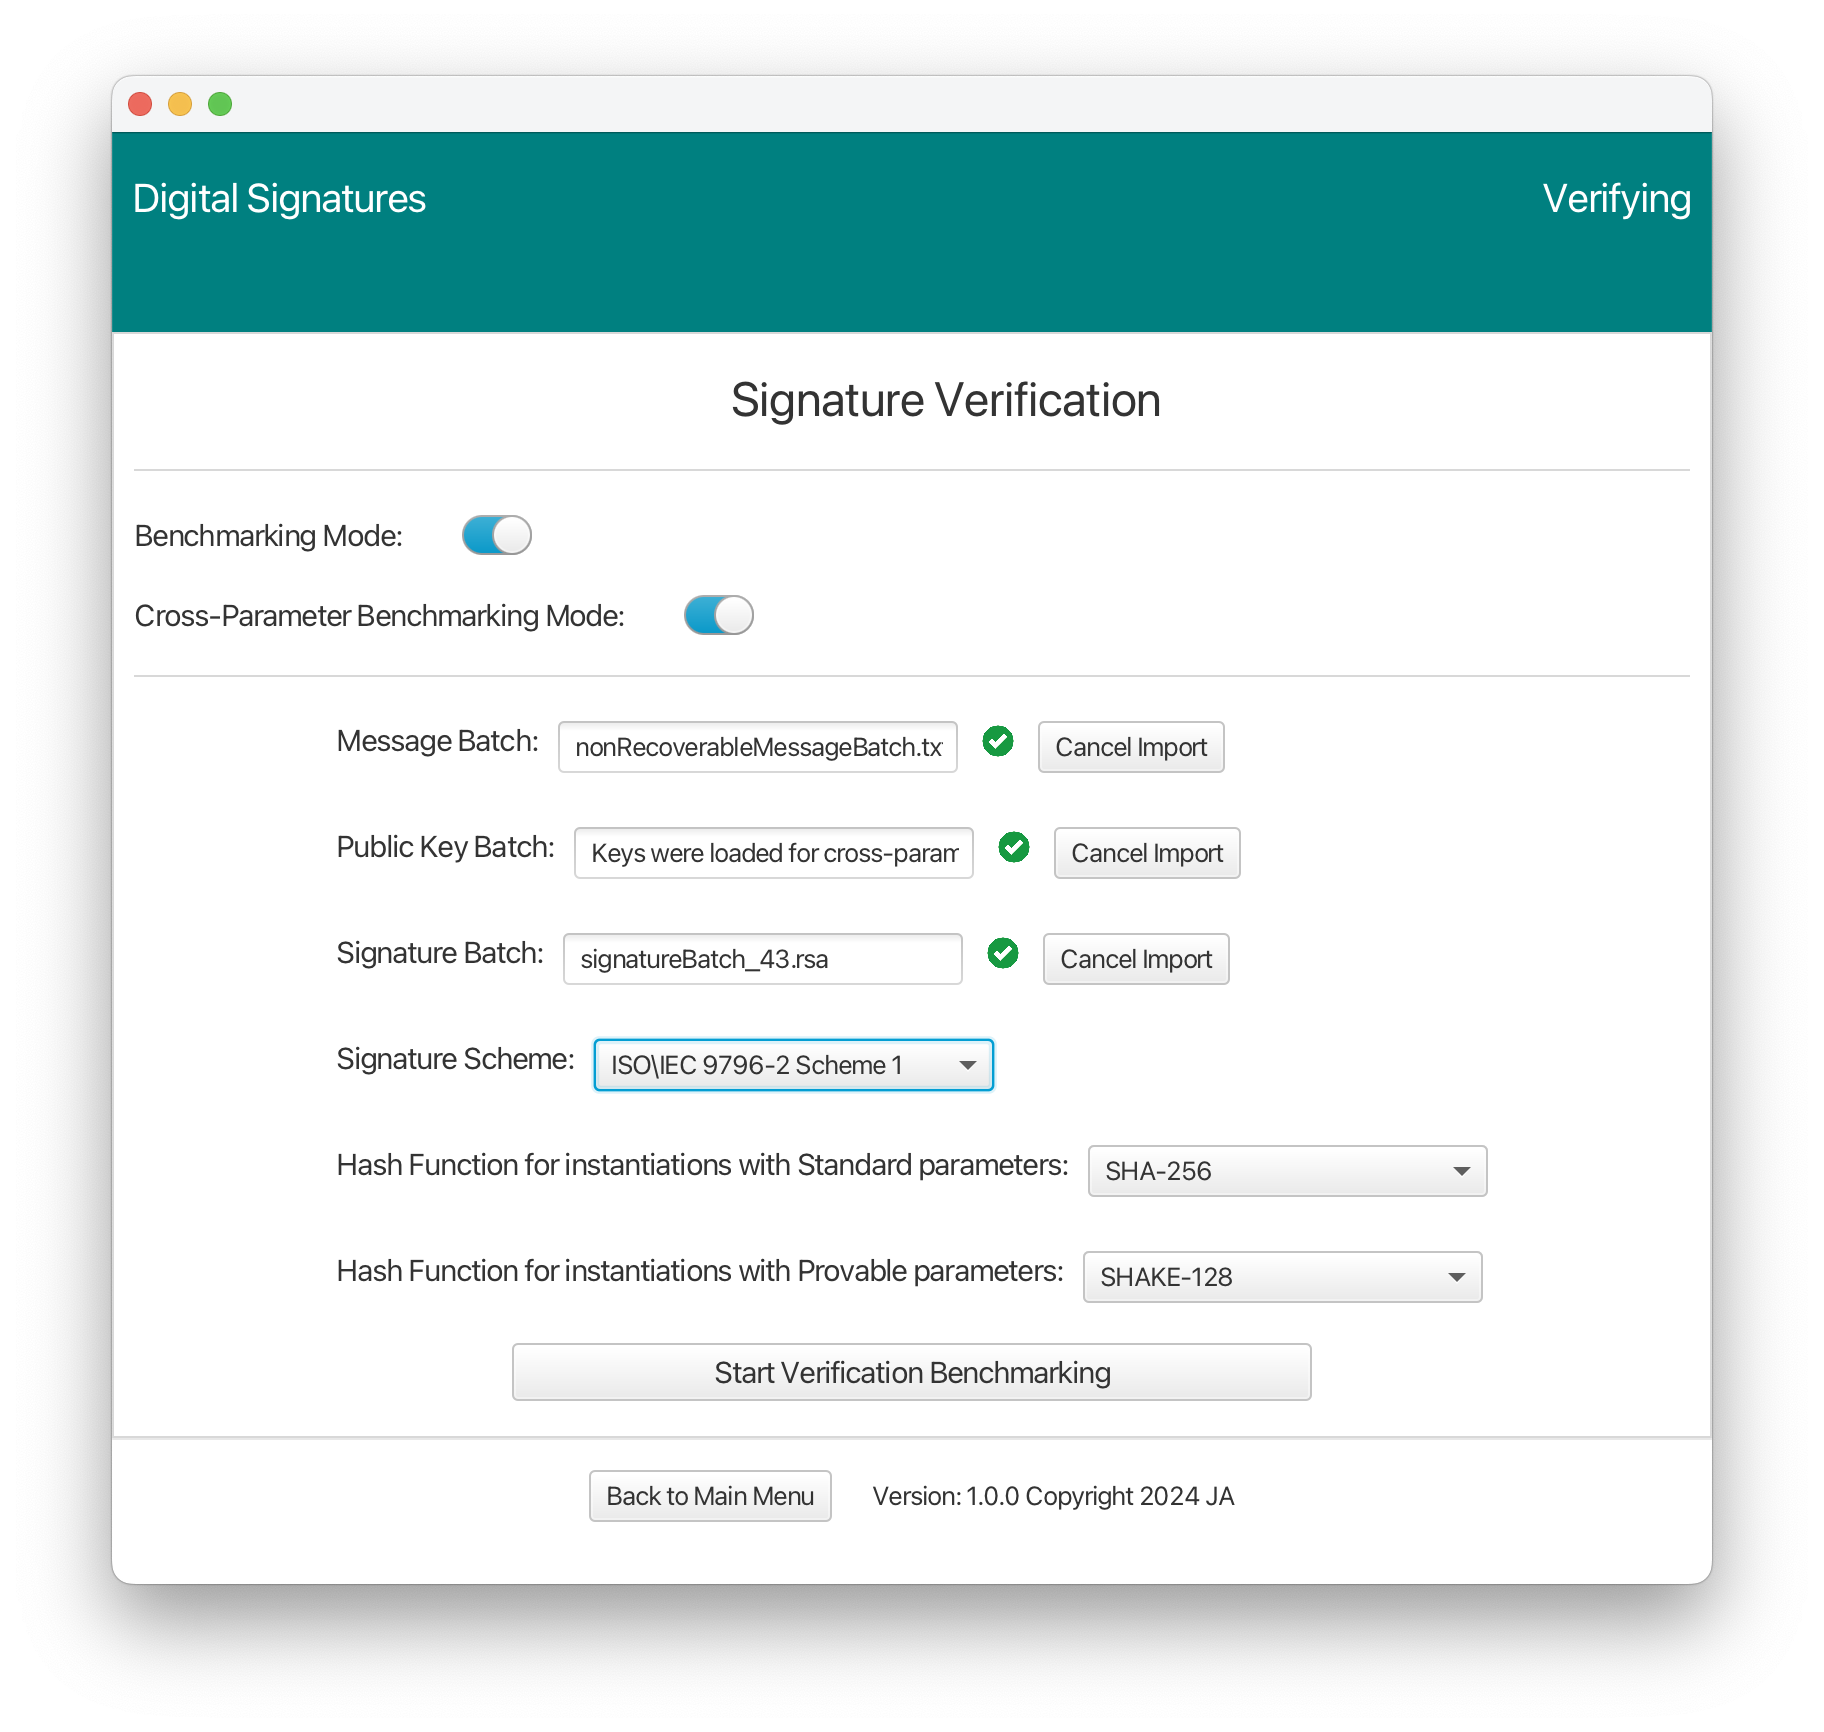
\includegraphics[width=\textwidth]{main_pictures/ui/verifying/verifying10.png}
    \caption{Comparison Benchmarking: Signature verification with ISO scheme selected}
\end{figure}

The corresponding verification of signatures necessitates import of a non-recoverable message batch file generated from the preceding signature generation benchmarking process. As discussed it contains entries aligned with each signature, organised line by line where each entry starts with a "1" or "0" flag, indicating whether a non-recoverable message part is present or absent, respectively. The application then leverages these non-recoverable message parts, to construct the content of a recovered message batch. This information is then displayed as a dedicated column in the verificationResults CSV files, which users can export for further analysis.


\textcolor{red} {
\begin{itemize}
\item For insight into the testing process see Appendix B.3 for more details.
\item For full code documentation in the form of javadoc, please see the application/docs/apidocs directory.
\end{itemize}
}
\begin{comment} (the the basis for many other de facto standards including ANSI X9, IETF, TLS) t \end{comment}
\chapter{Professional Issues: Adherence to Standards in Cryptography}



A standard is an established set of guidelines or specifications that provide recommendations for processes, practices, or systems. They are internationally agreed ways of working make technology more secure and interoperable \cite{isoCryptography2024}. In fact the most common mechanism for determining an appropriate cryptographic primitive, scheme or parameter choice is to consult a standard. 

The evolution of cryptography from military to commercial applications created a demand for standardisation in the area. There are thus an extensive range of international standards related to cryptography.  Of most pertinence to the signature schemes considered in this project we have the following three:
\begin{itemize}

\item \textit{\textbf{PKCS\# 1 (\cite{rfc8017})}} 
foundational RSA standard that outlines the mathematical properties and structure of RSA public and private keys. It also defines basic algorithms, encoding methods, and padding schemes necessary for RSA primitives.
\item \textit{\textbf{ANSI X9.31 (\cite{ANSI-1998-X9-31})}} is a now withdrawn United States financial industry standard for digital signatures based on the RSA algorithm.
\item \textit{\textbf{ISO/IEC 9796-2 (\cite{ISO/2010/9796-2-2010})}} defines three different RSA signature schemes that support message recovery including Digital Signature 1 which is used in the EMV payment system (provides a “platform” for enabling a chip card to be used in banking applications).
\end{itemize}

The demand for standards in cryptography has supplanted the traditional practice of security through obscurity, where keeping algorithmic details secret was the norm. Today, these details are open to the public, inviting scrutiny and evaluation from the international community of cryptographic researchers. This open approach assures that by the time an algorithm is integrated into a standard, it has withstood the rigours of peer evaluation, instilling confidence in developers who rely on these standards for secure application development.

Standards distill theoretical cryptographic techniques into clear guidelines covering implementation, appropriate contexts for use, and selection of algorithm parameters. They effectively bridge the gap between cryptographers, who typically have a deep understanding of mathematical theory but may lack practical software development experience, and software developers, who often lack extensive knowledge in cryptography.

This delineation of responsibilities ensures that each group can focus on their area of expertise while relying on shared, vetted practices. Standards in cryptography thus serve as a common language, enabling developers to adopt secure algorithms without needing to understand their theoretical underpinnings fully.


The world of cryptography offers numerous instances where implementations found not to follow standards correctly led to critical vulnerabilities \cite{4223237, 10.1145/2382196.2382205, 10.1145/2382196.2382204,  bleichenbacher1998chosen}. Among these, the Bleichenbacher signature forgery attacks \cite{finney2006bleichenbacher, kuhn2008variants} stands out as a prime example. This class of attacks, which worked on vulnerable implementations of the PKCS\#1 signature scheme, showcased the potential for serious security breaches. A real-world example targeting Facebook  \cite{bock2018return} in 2018 underscored the risk and during the same period, had been found to be affecting almost a third of the top 100 domains in the Alexa Top 1 Million list. Going further, such was severity of the threat, that a server could potentially be impersonated without accessing its private key. This starkly demonstrate how deviations from standards can lead to severe security breaches, and emphasises how it should be professional responsibility to implement these standards correctly.


In the context of this project, a key consideration was adhering to the standards defining the implemented signature schemes. It was paramount, not only to ensure that my initial implementations of these schemes conformed to the respective standards delineating them, but also to ensure that any modifications made for incorporating provably secure parameters aligned with established standards.

For example considering the latter, the first change included implementing  signatures to use RSA keys with a non-standard number of primes (three instead of two), which the PKCS\#1 standard already readily accommodates by defining the modulus N as a product of two or more primes. Another adjustment was the use of a large hash size ($\geq \lambda/2$). Although not directly addressed in the three standards for use in the signature schemes, standardised solutions are available as per the use of variable length hash functions for other use cases.  I adopted two of the most established methods for this: one being the MGF1 construction detailed in the PKCS\#1 standard \cite{rfc8017} and the other being the Keccak-based SHAKE hash functions (standardised by NIST in FIPS 202 \cite{1421}), both of which allow for variable length output. These adaptations ensured the project stayed within the bounds of established cryptographic standards. 

Furthermore, it was important for me that alignment with standards was to be achieved in a manner that was both ethical and practical. Since cryptographic algorithms are almost always necessary for securing sensitive data that might be communicated or stored, implementation of cryptographic standards, therefore, transcends mere technical expertise. It encompasses a broader professional and ethical responsibility towards safeguarding data and protecting privacy. This responsibility becomes increasingly significant in the current era where data breaches and cyberattacks are commonplace. Thus the approach of attempting to adhere to cryptographic standards I did not view simply a professional mandate but also as an ethical imperative to uphold the integrity and security of digital systems. This holds even in the context of my project which while academic, strived to emulate real-world conditions and implement actual signature schemes.
Throughout the project, I was cognisant of these factors and took steps to ensure that my implementations and modifications did not stray significantly from the path charted by the standards.

One example of a hurdle I faced was the foremost one: obtaining the required documentation for the standards related to schemes. Specifically, accessing the ANSI X9.31 and ISO/IEC 9796-2 standards was difficult as they are not publicly available, and ISO/IEC standards, in general, are often not freely accessible and can be costly.

Fortunately, the BSI website offers free access to ISO/IEC standards for students at institutions with subscriptions. As Royal Holloway has such a subscription \cite{BSIWebsite}, I was able to obtain the ISO/IEC 9796-2 standard. Meanwhile, the PKCS\#1 standard was readily available as it is published as part of the Internet Engineering Task Force's (IETF) RFC (Request for comments) series, specifically as RFC 8017 \cite{rfc8017}.

Addressing the issue with ANSI X9.31, which is a deprecated standard and hence not publicly available, required a different approach. I turned to peer-reviewed academic research papers that detailed the ANSI X9.31 implementation \cite{10.1007/978-3-030-64357-7_5}. These papers, while providing more of a high-level overview, aided me building in understanding the scheme. This then allowed me to leverage the similarities between ANSI X9.31 and PKCS\#1, both being variants of the signature schemes with appendix class. Using insights provided by the PKCS\#1 standard, I was able to address the implementation details that the academic papers did not fully cover. Furthermore the PKCS\#1 standard provided a reference for updating the implementation of the ANSI X9.31 scheme to reflect current cryptographic practices not available at the time the ANSI X9.31 standard was devised. 








\chapter{Results and Discussion}

\section{Setup and Methodology}
In order to compare the timing differential between standard and provably secure parameters, multiple disparate benchmarking runs were initiated in comparison benchmarking mode through the key generation portal for 6 key sizes increasing in 1024-bit segments from 1024-bit to 6144-bit. The number of trials for benchmarking was set to 3847 (which is the control variable used for every key configuration across key generation and signature creation/verification) to observe the behaviour of time taken. This specific number is related to the number of trials (messages) in the message batch that was used in benchmarking of the signature schemes.

\subsection{Dataset}

\begin{figure}[H]
    \centering
    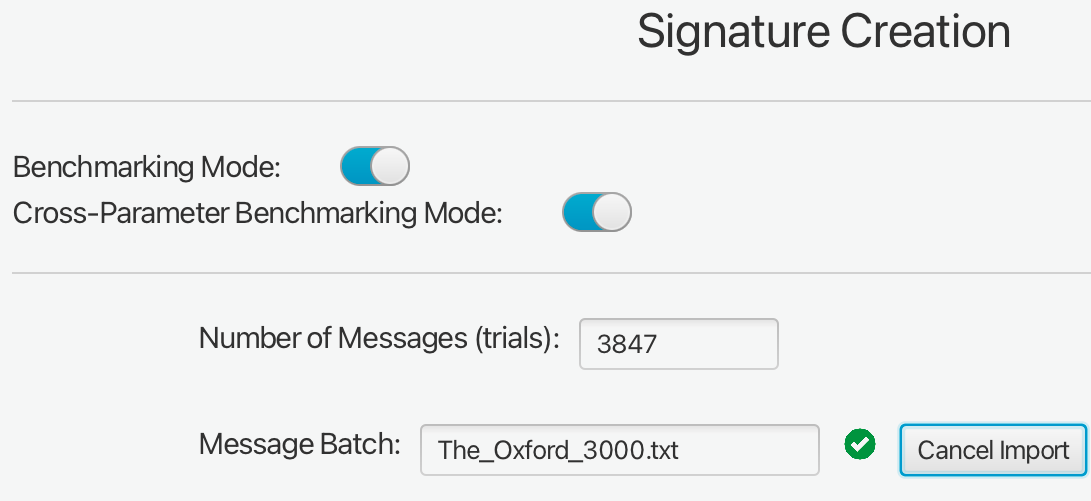
\includegraphics[width=\textwidth]{main_pictures/ui/dataset.png}
    \caption{Example of Oxford 3000 Dataset being imported for benchmarking}
\end{figure}

The dataset employed for the benchmarking of Signature Creation and Verification was derived from the first edition of the Oxford 3000 (2017) \cite{Oxford3000_2022}, a collection of the 3847 most important words to learn in English, as defined by the Oxford University Press. This dataset was utilised as the message batch taken from a text file representation of the list \cite{Oxford3000_GitHub} publicly available on GitHub. The aim was for each word/line from the Oxford 3000 list to serve as an individual message for processing through the signature schemes. The size of this dataset, with its 3847 entries, served as the control variable applied for every key configuration as its number of trials. 

\begin{comment}
By using this dataset, the benchmarking aimed to replicate realistic scenarios where such commonly used words might be part of digital communications that require digital signature operations. The size of the Oxford 3000 was appropriately large enough to provide substantial data for processing, yet manageable enough for a benchmarking exercise, helping to find balance to ensure that the benchmarking was comprehensive but not overly time-consuming or resource-intensive.
\end{comment}


\subsection{Hash function selection}

\begin{figure}[H]
    \centering 
    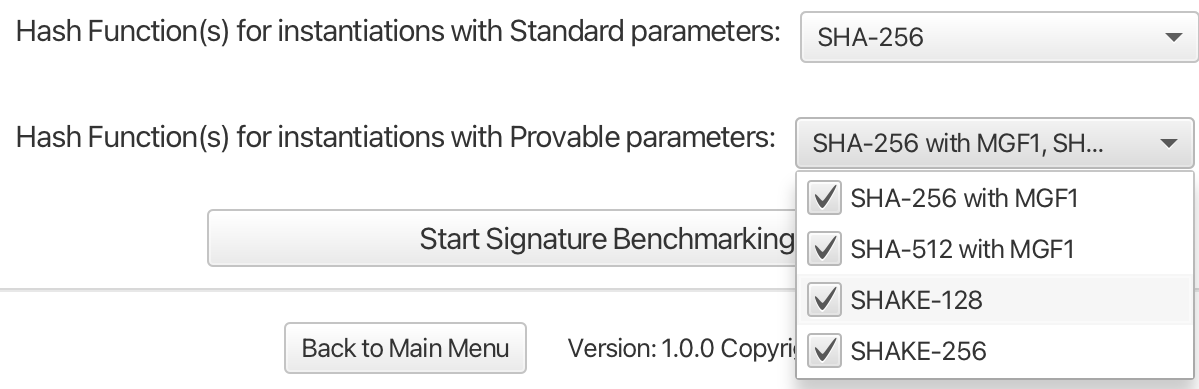
\includegraphics[width=\textwidth]{main_pictures/ui/hashChoices.png}
    \caption{Hash function selections respective to each parameter type used for benchmarking}
\end{figure}

\begin{comment}
For purposes of the comparative benchmarking, SHA-256 was selected as the hash function for instantiation of the schemes with standard parameters. Endorsed by the National Institute of Standards and Technology (NIST) as the minimum acceptable standard, SHA-256 is the most commonly utilised hash function thanks to its balance of performance and security. These reasons make it apt for representing standard instantiation of the considered signature schemes. 

For the instantiation of schemes with provably secure parameters, all variable-length hash functions available in the application were selected. This choice aimed to ensure that all types of provably secure instantiations could be accounted for in the subsequent analysis and allow deeper inspection into the implications of using provably secure parameters.
\end{comment}


\subsection{Hardware Specifications}
The following hardware specifications outline the computing environment used for all benchmarking exercises:
\begin{itemize}
\begin{comment} \item \textbf{Model:} Macbook Pro 14' (2021) \end{comment}
\item \textbf{Operating System:} macOS Sonoma 14.3.1
\item \textbf{CPU:} Apple M1 Pro
\item \textbf{Total Number of Cores:} 10 (8 performance and 2 efficiency)
\item \textbf{Clock Speed:} 3220 MHz (and 2064 MHz for Efficiency Cores)
\item \textbf{Instruction set:} ARMv8-A64 (64 bit)
\item \textbf{Memory:} 32 GB (LPDDR5 RAM)
\end{itemize}

The selected hardware represents a modern consumer-grade computing environment. Therefore, the results obtained from the benchmarking are indicative of the performance one might expect in similar settings.

\begin{comment}
It's important to note, that the considered deterministic schemes, often operate in environments vastly different from this testing setup which constitutes a modern computing environment. These include constrained legacy devices or low-performance environments, such as those found in payment/banking systems (e.g., EMV chip-and-pin cards) and secure network protocols.  Consequently benchmarking results may not be fully applicable or generalisable to the diverse range of use cases where these older schemes are still operational.  
\end{comment}
\begin{comment}

While the benchmarking results provide valuable insights into the performance of cryptographic operations on modern hardware, they may not be fully applicable or generalisable to the diverse range of use cases where these older schemes are still operational. Therefore, caution should be exercised when interpreting these results outside the specific context of the testing environment.
\end{comment}

\section{Results}
The timing results for key generation, signature creation, and verification across each deterministic signature scheme were captured using the developed application. These results are summarised in tables presented in textual format. These tables were generated from CSV exports file provided by and corresponding with the tables displayed on the application’s results screen when benchmarking was performed.


\textit{*For the views of the complete result tables and subsequent breakdown by parameter type, specific to the ANSI X9.31 rDSA and ISO/IEC 9796-2:2010 Signature Schemes, please consult Appendix D.} 


\begin{landscape}
\pagestyle{empty}%

\section{Key Generation Results}

%TC:ignore
\begin{table}[H]
\caption{\textbf{Standard vs Provably Secure Key Configurations for 1024-bit Key Size}}
\centering

\begin{tabular}{|p{2.5cm}|p{1cm}|p{1.5cm}|p{1.5cm}|p{1.3cm}|p{1.5cm}|p{2.5cm}|p{1.5cm}|p{1.5cm}|p{1.5cm}|p{1.5cm}|p{1.5cm}|p{1.5cm}|}

\hline
\textbf{Parameter Type} & \textbf{Trials} & \textbf{Overall Time} & \textbf{Mean} & \textbf{Std Dev} & \textbf{Variance} & \textbf{Conf. Interval} & \textbf{25th Percentile} & \textbf{Median} & \textbf{75th Percentile} & \textbf{Range} & \textbf{Min} & \textbf{Max} \\
\hline
Standard Parameters (2 Primes) & 3847 & 32500.
03302 ms & 8.44815 ms & 3.06326 ms & 9.38357 ms\textsuperscript{2} & 95\% [8.35135 ms - 8.54495 ms] & 6.45296 ms & 7.93108 ms & 9.81196 ms & 109.36288 ms & 4.48542 ms & 113.84
829 ms \\
\hline
Standard Parameters (3 Primes) & 3847 & 25971.
95539 ms & 6.75122 ms & 2.77931 ms & 7.72459 ms\textsuperscript{2} & 95\% [6.66340 ms - 6.83905 ms] & 5.04292 ms & 6.25900 ms & 7.93117 ms & 110.15567 ms & 3.46463 ms & 113.62
029 ms \\
\hline
Provable Parameters (2 Primes) & 3847 & 31838.
01822 ms & 8.27606 ms & 2.98431 ms & 8.90612 ms\textsuperscript{2} & 95\% [8.18176 ms - 8.37037 ms] & 6.27650 ms & 7.78642 ms & 9.73663 ms & 98.98717 ms & 4.30804 ms & 103.29
521 ms \\
\hline
Provable Parameters (3 Primes) & 3847 & 24060.
58383 ms & 6.25438 ms & 2.58707 ms & 6.69292 ms\textsuperscript{2} & 95\% [6.17262 ms - 6.33613 ms] & 4.61788 ms & 5.72271 ms & 7.32038 ms & 100.38979 ms & 3.45338 ms & 103.84
317 ms \\
\hline
\end{tabular}
    \label{keyGen_1024bit_table}
\end{table}

\begin{table}[H]
\caption{\textbf{Standard vs Provably Secure Key Configurations for 2048-bit Key Size}}
\centering

\begin{tabular}{|p{2.5cm}|p{1cm}|p{1.5cm}|p{1.5cm}|p{1.3cm}|p{1.5cm}|p{2.5cm}|p{1.5cm}|p{1.5cm}|p{1.5cm}|p{1.5cm}|p{1.5cm}|p{1.6cm}|}

\hline
\textbf{Parameter Type} & \textbf{Trials} & \textbf{Overall Time} & \textbf{Mean} & \textbf{Std Dev} & \textbf{Variance} & \textbf{Conf. Interval} & \textbf{25th Percentile} & \textbf{Median} & \textbf{75th Percentile} & \textbf{Range} & \textbf{Min} & \textbf{Max} \\
\hline
Standard Parameters (2 Primes) & 3847 & 216832.
70813 ms & 56.36410 ms & 25.11093 ms & 630.
55905 ms\textsuperscript{2} & 95\% [55.57060 ms - 57.15761 ms] & 38.30242 ms & 50.84733 ms & 69.46363 ms & 251.96708 ms & 20.66575 ms & 272.63283 ms \\
\hline
Standard Parameters (3 Primes) & 3847 & 142789.
88957 ms & 37.11721 ms & 18.77580 ms & 352.
53051 ms\textsuperscript{2} & 95\% [36.52389 ms - 37.71052 ms] & 24.18892 ms & 31.63142 ms & 43.91163 ms & 149.11308 ms & 15.19508 ms & 164.30817 ms \\
\hline
Provable Parameters (2 Primes) & 3847 & 211874.
31649 ms & 55.07521 ms & 25.43492 ms & 646.
93532 ms\textsuperscript{2} & 95\% [54.27146 ms - 55.87895 ms] & 36.39042 ms & 48.82779 ms & 67.61679 ms & 225.86154 ms & 19.86850 ms & 245.73004 ms \\
\hline
Provable Parameters (3 Primes) & 3847 & 140797.
38616 ms & 36.59927 ms & 18.11657 ms & 328.
21007 ms\textsuperscript{2} & 95\% [36.02679 ms - 37.17175 ms] & 23.74371 ms & 31.40804 ms & 43.76967 ms & 164.12904 ms & 14.48221 ms & 178.61125 ms \\
\hline
\end{tabular}
\label{keyGen_2048bit_table}
\end{table}
\begin{table}[H]
\caption{\textbf{Standard vs Provably Secure Key Configurations for 3072-bit Key Size}}
\centering

\begin{tabular}{|p{2.5cm}|p{1cm}|p{1.5cm}|p{1.5cm}|p{1.3cm}|p{1.5cm}|p{2.5cm}|p{1.5cm}|p{1.5cm}|p{1.5cm}|p{1.5cm}|p{1.5cm}|p{1.6cm}|}

\hline
\textbf{Parameter Type} & \textbf{Trials} & \textbf{Overall Time} & \textbf{Mean} & \textbf{Std Dev} & \textbf{Variance} & \textbf{Conf. Interval} & \textbf{25th Percentile} & \textbf{Median} & \textbf{75th Percentile} & \textbf{Range} & \textbf{Min} & \textbf{Max} \\
\hline
Standard Parameters (2 Primes) & 3847 & 859374.
27891 ms & 223.38817 ms & 110.
51449 ms & 12213.
45183 ms\textsuperscript{2} & 95\% [219.89591 ms - 226.88042 ms] & 141.93146 ms & 201.04146 ms & 278.57204 ms & 890.91733 ms & 66.01350 ms & 956.93083 ms \\
\hline
Standard Parameters (3 Primes) & 3847 & 522259.
93065 ms & 135.75772 ms & 79.
61435 ms & 6338.
44448 ms\textsuperscript{2} & 95\% [133.24190 ms - 138.27353 ms] & 79.61400 ms & 111.80900 ms & 167.72454 ms & 682.03238 ms & 42.99892 ms & 725.03129 ms \\
\hline
Provable Parameters (2 Primes) & 3847 & 935726.
17065 ms & 243.23529 ms & 116.
81273 ms & 13645.
21423 ms\textsuperscript{2} & 95\% [239.54401 ms - 246.92657 ms] & 157.94288 ms & 219.19454 ms & 303.23038 ms & 1007.12354 ms & 69.48767 ms & 1076.61121 ms \\
\hline
Provable Parameters (3 Primes) & 3847 & 586821.
93877 ms & 152.54015 ms & 89.
76538 ms & 8057.82387 ms\textsuperscript{2} & 95\% [149.70356 ms - 155.37673 ms] & 88.34038 ms & 125.12150 ms & 189.
92954 ms & 732.55608 ms & 42.01850 ms & 774.57458 ms \\
\hline
\end{tabular}
\label{keyGen_3072bit_table}
\end{table}
\begin{table}[H]
\caption{\textbf{Standard vs Provably Secure Key Configurations for 4096-bit Key Size}}
\centering

\begin{tabular}{|p{2.5cm}|p{1cm}|p{1.5cm}|p{1.5cm}|p{1.5cm}|p{1.5cm}|p{2.5cm}|p{1.5cm}|p{1.5cm}|p{1.5cm}|p{1.5cm}|p{1.5cm}|p{1.65cm}|}

\hline
\textbf{Parameter Type} & \textbf{Trials} & \textbf{Overall Time} & \textbf{Mean} & \textbf{Std Dev} & \textbf{Variance} & \textbf{Conf. Interval} & \textbf{25th Percentile} & \textbf{Median} & \textbf{75th Percentile} & \textbf{Range} & \textbf{Min} & \textbf{Max} \\
\hline
Standard Parameters (2 Primes) & 3847 & 2512465.
59783 ms & 653.09737 ms & 349.82224 ms & 122375.
60291 ms\textsuperscript{2} & 95\% [642.04299 ms - 664.15175 ms] & 394.05558 ms & 568.76025 ms & 823.37171 ms & 2480.62675 ms & 156.76954 ms & 2637.39629 ms \\
\hline
Standard Parameters (3 Primes) & 3847 & 1524916.
73096 ms & 396.39114 ms & 244.54868 ms & 59804.
05520 ms\textsuperscript{2} & 95\% [388.66341 ms - 404.11888 ms] & 220.45496 ms & 326.98117 ms & 497.99713 ms & 2063.10838 ms & 103.00438 ms & 2166.11275 ms \\
\hline
Provable Parameters (2 Primes) & 3847 & 2494789.
87108 ms & 648.50270 ms & 340.86642 ms & 116189.
91836 ms\textsuperscript{2} & 95\% [637.73132 ms - 659.27407 ms] & 396.17483 ms & 577.23179 ms & 823.48121 ms & 2562.00825 ms & 144.18433 ms & 2706.19258 ms \\
\hline
Provable Parameters (3 Primes) & 3847 & 1516030.
63440 ms & 394.08127 ms & 251.03722 ms & 63019.
68474 ms\textsuperscript{2} & 95\% [386.14849 ms - 402.01404 ms] & 218.82379 ms & 318.45613 ms & 490.04521 ms & 1877.85863 ms & 99.98625 ms & 1977.84488 ms \\
\hline
\end{tabular}
\label{keyGen_4096bit_table}
\end{table}

\begin{table}[H]
\caption{\textbf{Standard vs Provably Secure Key Configurations for 5120-bit Key Size}}
\centering

\begin{tabular}{|p{2.5cm}|p{1cm}|p{1.5cm}|p{1.5cm}|p{1.5cm}|p{1.5cm}|p{2.5cm}|p{1.5cm}|p{1.75cm}|p{1.6cm}|p{1.5cm}|p{1.5cm}|p{1.55cm}|}

\hline
\textbf{Parameter Type} & \textbf{Trials} & \textbf{Overall Time} & \textbf{Mean} & \textbf{Std Dev} & \textbf{Variance} & \textbf{Conf. Interval} & \textbf{25th Percentile} & \textbf{Median} & \textbf{75th Percentile} & \textbf{Range} & \textbf{Min} & \textbf{Max} \\
\hline
Standard Parameters (2 Primes) & 3847 & 5139570.
81048 ms & 1335.
99449 ms & 768.65487 ms & 590830.
30418 ms\textsuperscript{2} & 95\% [1311.70500 ms - 1360.28398 ms] & 764.87479 ms & 1181.51417 ms & 1742.
38763 ms & 6430.
46850 ms & 213.62488 ms & 6644.
09338 ms \\
\hline
Standard Parameters (3 Primes) & 3847 & 3127106.
74416 ms & 812.
86892 ms & 581.48345 ms & 338123.
00804 ms\textsuperscript{2} & 95\% [794.49405 ms - 831.24380 ms] & 406.25875 ms & 644.99658 ms & 1035.
09046 ms & 6498.
48363 ms & 149.57371 ms & 6648.
05733 ms \\
\hline
Provable Parameters (2 Primes) & 3847 & 5177297.
05958 ms & 1345.
80116 ms & 789.79128 ms & 623770.
26124 ms\textsuperscript{2} & 95\% [1320.84376 ms - 1370.75856 ms] & 757.04067 ms & 1157.88358 ms & 1740.
98383 ms & 5979.
87283 ms & 216.35467 ms & 6196.
22750 ms \\
\hline
Provable Parameters (3 Primes) & 3847 & 3096978.
48924 ms & 805.
03730 ms & 555.58792 ms & 308677.
94012 ms\textsuperscript{2} & 95\% [787.48072 ms - 822.59387 ms] & 409.86204 ms & 636.65933 ms & 1035.
07746 ms & 4388.
49479 ms & 156.91004 ms & 4545.
40483 ms \\
\hline
\end{tabular}
\label{keyGen_5120bit_table}
\end{table}

\begin{table}[H]
\caption{\textbf{Standard vs Provably Secure Key Configurations for 6144-bit Key Size}}
\centering

\begin{tabular}{|p{2.5cm}|p{1cm}|p{1.5cm}|p{1.6cm}|p{1.3cm}|p{1.5cm}|p{2.5cm}|p{1.5cm}|p{1.38cm}|p{1.7cm}|p{1.5cm}|p{1.5cm}|p{1.7cm}|}

\hline
\textbf{Parameter Type} & \textbf{Trials} & \textbf{Overall Time} & \textbf{Mean} & \textbf{Std Dev} & \textbf{Variance} & \textbf{Conf. Interval} & \textbf{25th Percentile} & \textbf{Median} & \textbf{75th Percentile} & \textbf{Range} & \textbf{Min} & \textbf{Max} \\
\hline
Standard Parameters (2 Primes) & 3847 & 10025508.
51280 ms & 2606.
05888 ms & 1614.
90918 ms & 2607931.
66202 ms\textsuperscript{2} & 95\% [2555.02776 ms - 2657.09000 ms] & 1417.
27975 ms & 2245.
02108 ms & 3422.26542 ms & 11525.
95642 ms & 341.26588 ms & 11867.
22229 ms \\
\hline
Standard Parameters (3 Primes) & 3847 & 5937935.
29067 ms & 1543.
52360 ms & 1162.
66910 ms & 1351799.
44484 ms\textsuperscript{2} & 95\% [1506.78326 ms - 1580.26394 ms] & 715.
96850 ms & 1207.
89275 ms & 1981.24696 ms & 8259.
66388 ms & 269.06354 ms & 8528.
72742 ms \\
\hline
Provable Parameters (2 Primes) & 3847 & 9976397.
40289 ms & 2593.
29280 ms & 1566.
57388 ms & 2454153.
70771 ms\textsuperscript{2} & 95\% [2543.78908 ms - 2642.79653 ms] & 1420.
57613 ms & 2256.
76554 ms & 3417.35108 ms & 10998.
30175 ms & 320.67396 ms & 11318.
97571 ms \\
\hline
Provable Parameters (3 Primes) & 3847 & 5899550.
30713 ms & 1533.
54570 ms & 1147.
96010 ms & 1317812.
38040 ms\textsuperscript{2} & 95\% [1497.27017 ms - 1569.82123 ms] & 721.
49154 ms & 1194.
99279 ms & 2007.73946 ms & 11288.
17233 ms & 224.15396 ms & 11512.
32629 ms \\
\hline
\end{tabular}
\label{keyGen_6144bit_table}
\end{table}

%TC:endignore

\end{landscape}


  
Tables \ref{keyGen_1024bit_table} to \ref{keyGen_6144bit_table} show timing statistics in milliseconds (correct to 5 decimal places) for both standard and provably secure key configurations across a range of key sizes, incrementing by 1024 bits from 1024 to 6144 bits. 


\textbf{Comparing 2 vs 3 primes within parameter groups}


Table \ref{tab:2vs3primes_percentage} illustrates the percentage difference in mean generation times when moving from 2-prime to 3-prime configurations for each parameter group. 

\begin{table}[H]
\centering
\caption{Efficiency Comparison of 2 vs 3 Primes in Key Generation (Percentage Difference)}
\begin{tabular}{|c|c|c|}
\hline
\textbf{Key Size (bits)} & \textbf{2 Primes to 3 Primes \% Diff} & \textbf{2 Primes to 3 Primes \% Diff} \\
 & \textbf{(Standard Parameters)} & \textbf{(Provably Secure Parameters)} \\
\hline
1024 & -20.07\% & -24.43\% \\
2048 & -34.17\% & -33.54\% \\
3072 & -39.22\% & -37.30\% \\
4096 & -39.30\% & -39.23\% \\
5120 & -39.16\% & -40.20\% \\
6144 & -40.77\% & -40.85\% \\
\hline
\end{tabular}
\label{tab:2vs3primes_percentage}
\end{table}

A consistent trend observed across all key sizes from 1024 to 6144 bits is the superior performance of 3-prime configurations over 2-prime configurations. This pattern holds true within both standard and provably secure parameter types. Notably, the efficiency advantage of 3-prime configurations also increased with key size.


\textbf{Comparing Standard vs provably secure key configurations}

The distinction of the pattern being within parameter types is an important one to make because it illustrates what appears to be an inherent efficiency gain in key generation when additional prime factors are used, irrespective of whether the parameters are standard or provably secure. For example, at the 1024-bit key size, while both provably secure configurations with 2 and 3 primes show a slight performance increase over their standard counterparts, comparing across different parameter types with a different number of primes (like 2 primes provably secure vs. 3 primes standard) is not equitable due to the fundamental difference in the configuration setup.

More concretely, at the 1024-bit key size \ref{keyGen_1024bit_table}, provably secure configurations with both 2 and 3 primes show modest efficiency gains over standard counterparts. Specifically, the provably secure 2-prime configuration was approximately 2.04\% quicker (8.27606 ms compared to 8.44815 ms), and the provably secure 3-prime configurations demonstrated a 7.35\% reduction in mean time (6.25438 ms versus 6.75122 ms). This trend challenges the usual belief that enhanced security compromises performance. Both configuration types exhibit relatively lower standard deviation and variance at this size, indicating consistent performance.

As key sizes increase, to 2048 bits \ref{keyGen_2048bit_table}, the pattern of improved efficiency in provably secure configurations compared to standard holds, with about 2\% faster mean time in the  2-prime configuration and 1.4\% in 3-prime configuration. However, at 3072 bits  \ref{keyGen_3072bit_table}, a deviation emerges: while the 3-prime provably secure configuration maintained a 12.3\% efficiency advantage, the  2-prime provably secure configuration bucked the trend coming in at 8.91\% slower than its standard counterpart. This size also marked a notable increase in standard deviation and variance, a suggestion of a wider spread in key generation times.

Moving to 4096-bit  and 5120-bit key sizes, provably secure configurations maintain their lead in efficiency over standard configurations, although the margin gets narrower. 

\begin{comment}
Specifically, at 4096 bits \ref{keyGen_4096bit_table}, the mean time for generating a key with a provably secure 2-prime configuration was marginally faster by 0.70\% (648.50270 ms) than the standard setup (653.09737 ms). The advantage is even slighter in the 3-prime category, with a 0.58\% quicker generation time (394.08127 ms for provably secure versus 396.39114 ms for standard).
At the 5120-bit Key Size \ref{keyGen_5120bit_table}, the provably secure 2-prime configuration was 1.38\% faster (1335.99449 ms compared to 1345.80116 ms for standard), while the 3-prime configuration was 0.96\% faster (805.03730 ms compared to 812.86892 ms for standard). The progressive deterioration in standard deviation and variance continued, hinting at greater variability and a potential overshadowing of the small efficiency gains.
 \end{comment}
 
At the largest tested size of 6144 bits \ref{keyGen_6144bit_table}, the efficiency gap remains minimal, with provably secure parameters showing only about 0.49\% and 0.64\% improvements for 2-prime and 3-prime configurations respectively. This key size experienced the highest standard deviation and variance, emphasising significant variability in key generation times.


\subsection*{Summary}
Throughout the analysis, as expected, the time taken for key generation increases with the key size. However, the increase is not linear; it tends to grow more than proportional, reflecting the greater computational complexity involved in generating and handling larger primes. This complexity becomes particularly evident through the marked rise in standard deviation and variance in larger key sizes for both standard and provably secure configurations.
While provably secure parameters exhibit some efficiency improvements, these gains are relatively minimal, especially as key sizes grow larger. The increased variability at larger key sizes, as indicated by higher standard deviation and variance, obscures the true impact of opting for provably secure parameters since the small percentage difference may fall within the broader range of natural variability of the key generation process. Consequently, although provably secure configurations show efficiency improvements at smaller key sizes, their practical significance wanes with increasing key sizes.

In essence, when considering solely the smaller value of e used in provably secure configurations as the distinguishing factor as compared to standard configurations, there is no significant difference in key generation between both types. Moreover the distinction between the two becomes negligible, with increasingly larger key sizes. 

However, if the increased number of primes (to three) used for both configuration types is taken into account, the results point towards a notable efficiency advantage for 3-prime configurations over 2-prime configurations across all key sizes. Notably, it's important to acknowledge that while the extra prime is utilised in both configuration types, its necessity stems also as implication of the proofs, so can thus be considered a form of provably secure key configuration in its own right. 

The counterintuitive results suggests that adopting provably secure parameters—which would have been presumed to be less efficient due to enhancing security— actually offer performance benefits. The first scenario reflecting minimal improvements at lower key sizes can attributed to the use of  a smaller e values. In the second scenario, there is an inherent and significant advantage of using 3-prime configurations over 2-prime configuration and one that that intensifies with increasing key size.





\begin{landscape}
\pagestyle{empty}%

\section{Signature Creation Results}
\subsection{Signature Creation Results (PKCS\#1 v1.5)}

%TC:ignore
\begin{longtable}{|p{2.3cm}|p{1.8cm}|p{1.0cm}|p{1.7cm}|p{1.2cm}|p{1.5cm}|p{1.8cm}|p{1.5cm}|p{1.2cm}|p{1.5cm}|p{1.3cm}|p{1.2cm}|p{1.3cm}|p{1.3cm}|}

\caption{\textbf{Instantiation of PKCS\#1 v1.5 with Standard vs Provably Secure Parameters (1024-bit Key Size) for Signature Creation}}
     \label{pkcs_sign_1024bit_table} \\
\hline
\textbf{Parameter Type} & \textbf{Hash Function} & \textbf{Trials} & \textbf{Overall Time} & \textbf{Mean} & \textbf{Std Dev} & \textbf{Variance} & \textbf{Conf. Interval} & \textbf{25th Percentile} & \textbf{Median} & \textbf{75th Percentile} & \textbf{Range} & \textbf{Min} & \textbf{Max} \\
\hline
\endfirsthead

\multicolumn{14}{c}%
{{\bfseries \tablename\ \thetable{} -- Signature Creation Results for PKCS\#1 v1.5 with 1024-bit Key Size (continued from previous page)}} \\
\hline
\textbf{Parameter Type} & \textbf{Hash Function} & \textbf{Trials} & \textbf{Overall Time} & \textbf{Mean} & \textbf{Std Dev} & \textbf{Variance} & \textbf{Conf. Interval} & \textbf{25th Percentile} & \textbf{Median} & \textbf{75th Percentile} & \textbf{Range} & \textbf{Min} & \textbf{Max} \\
\hline
\endhead

\hline \multicolumn{14}{|r|}{{Continued on next page}} \\ \hline
\endfoot

\hline
\endlastfoot

Standard Parameters (2 Primes) & SHA-256 & 3847 & 118177.
02163 ms & 30.
71927 ms & 33.07081 ms & 1093.
67843 ms\textsuperscript{2} & 95\% [29.67423 ms - 31.76430 ms] & 3.03771 ms & 22.12350 ms & 50.83954 ms & 140.
51642 ms & 0.42242 ms & 140.
93883 ms \\
\hline
Standard Parameters (3 Primes) & SHA-256 & 3847 & 115791.
12898 ms & 30.
09907 ms & 31.
98768 ms & 1023.21183 ms\textsuperscript{2} & 95\% [29.08826 ms - 31.10988 ms] & 3.03488 ms & 18.00500 ms & 50.58250 ms & 118.
82333 ms & 0.42608 ms & 119.
24942 ms \\
\hline
Provable Parameters (2 Primes) & SHA-256 with MGF1 (512bit) & 3847 & 115272.
70898 ms & 29.
96431 ms & 31.
73466 ms & 1007.08866 ms\textsuperscript{2} & 95\% [28.96150 ms - 30.96713 ms] & 3.03171 ms & 18.21867 ms & 50.26879 ms & 113.
74892 ms & 0.42229 ms & 114.
17121 ms \\
\hline
Provable Parameters (3 Primes) & SHA-256 with MGF1 (512bit) & 3847 & 115671.
24224 ms & 30.
06791 ms & 31.
83358 ms & 1013.37703 ms\textsuperscript{2} & 95\% [29.06197 ms - 31.07385 ms] & 3.03213 ms & 17.74683 ms & 50.27175 ms & 125.
09771 ms & 0.42179 ms & 125.
51950 ms \\
\hline
Provable Parameters (2 Primes) & SHA-512 with MGF1 (512bit) & 3847 & 116170.
35977 ms & 30.
19765 ms & 31.
86701 ms & 1015.50602 ms\textsuperscript{2} & 95\% [29.19065 ms - 31.20465 ms] & 3.03246 ms & 22.24804 ms & 50.72604 ms & 116.
11454 ms & 0.42108 ms & 116.
53563 ms \\
\hline
Provable Parameters (3 Primes) & SHA-512 with MGF1 (512bit) & 3847 & 115125.
70527 ms & 29.
92610 ms & 31.
58010 ms & 997.30245 ms\textsuperscript{2} & 95\% [28.92817 ms - 30.92403 ms] & 3.03092 ms & 22.40379 ms & 50.36567 ms & 114.
46588 ms & 0.42367 ms & 114.
88954 ms \\
\hline
Provable Parameters (2 Primes) & SHAKE-128 (512bit) & 3847 & 115843.
34085 ms & 30.
11264 ms & 31.
82802 ms & 1013.02270 ms\textsuperscript{2} & 95\% [29.10688 ms - 31.11841 ms] & 3.03104 ms & 22.11000 ms & 50.45063 ms & 124.
24679 ms & 0.42171 ms & 124.
66850 ms \\
\hline
Provable Parameters (3 Primes) & SHAKE-128 (512bit) & 3847 & 116287.
14955 ms & 30.
22801 ms & 31.
88017 ms & 1016.34492 ms\textsuperscript{2} & 95\% [29.22060 ms - 31.23542 ms] & 3.03183 ms & 22.40679 ms & 50.35983 ms & 133.
25854 ms & 0.42046 ms & 133.
67900 ms \\
\hline
Provable Parameters (2 Primes) & SHAKE-256 (512bit) & 3847 & 116012.
33564 ms & 30.
15657 ms & 31.
81386 ms & 1012.12174 ms\textsuperscript{2} & 95\% [29.15126 ms - 31.16189 ms] & 3.03171 ms & 21.99000 ms & 50.58658 ms & 122.
58917 ms & 0.42133 ms & 123.
01050 ms \\
\hline
Provable Parameters (3 Primes) & SHAKE-256 (512bit) & 3847 & 115285.
59635 ms & 29.
96766 ms & 31.
57840 ms & 997.19519 ms\textsuperscript{2} & 95\% [28.96978 ms - 30.96554 ms] & 3.03167 ms & 18.76663 ms & 50.47438 ms & 119.
35754 ms & 0.42046 ms & 119.
77800 ms \\
\hline

\end{longtable}


\begin{longtable}{|p{2.3cm}|p{1.8cm}|p{1.0cm}|p{1.7cm}|p{1.2cm}|p{1.5cm}|p{1.8cm}|p{1.5cm}|p{1.2cm}|p{1.5cm}|p{1.3cm}|p{1.2cm}|p{1.3cm}|p{1.3cm}|}

\caption{\textbf{Instantiation of PKCS\#1 v1.5 with Standard vs Provably Secure Parameters (2048-bit Key Size) for Signature Creation}}
     \label{pkcs_sign_2048bit_table} \\
\hline
\textbf{Parameter Type} & \textbf{Hash Function} & \textbf{Trials} & \textbf{Overall Time} & \textbf{Mean} & \textbf{Std Dev} & \textbf{Variance} & \textbf{Conf. Interval} & \textbf{25th Percentile} & \textbf{Median} & \textbf{75th Percentile} & \textbf{Range} & \textbf{Min} & \textbf{Max} \\
\hline
\endfirsthead

\multicolumn{14}{c}%
{{\bfseries \tablename\ \thetable{} -- Signature Creation Results for PKCS\#1 v1.5 with 2048-bit Key Size (continued from previous page)}} \\
\hline
\textbf{Parameter Type} & \textbf{Hash Function} & \textbf{Trials} & \textbf{Overall Time} & \textbf{Mean} & \textbf{Std Dev} & \textbf{Variance} & \textbf{Conf. Interval} & \textbf{25th Percentile} & \textbf{Median} & \textbf{75th Percentile} & \textbf{Range} & \textbf{Min} & \textbf{Max} \\
\hline
\endhead

\hline \multicolumn{14}{|r|}{{Continued on next page}} \\ \hline
\endfoot

\hline
\endlastfoot

Standard Parameters (2 Primes) & SHA-256 (1024bit) & 3847 & 115894.
04309 ms & 30.
12582 ms & 31.83583 ms & 1013.
51994 ms\textsuperscript{2} & 95\% [29.11981 ms - 31.13184 ms] & 3.03108 ms & 18.60683 ms & 50.49133 ms & 117.
63146 ms & 0.42183 ms & 118.
05329 ms \\
\hline
Standard Parameters (3 Primes) & SHA-256 (1024bit) & 3847 & 116100.
80914 ms & 30.
17957 ms & 31.75342 ms & 1008.
27967 ms\textsuperscript{2} & 95\% [29.17616 ms - 31.18298 ms] & 3.03263 ms & 19.40667 ms & 50.79829 ms & 140.
20000 ms & 0.42175 ms & 140.
62175 ms \\
\hline
Provable Parameters (2 Primes) & SHA-256 with MGF1 (1024bit) & 3847 & 116078.
59544 ms & 30.
17380 ms & 31.89360 ms & 1017.
20177 ms\textsuperscript{2} & 95\% [29.16596 ms - 31.18163 ms] & 3.03221 ms & 22.03592 ms & 50.46375 ms & 143.
56496 ms & 0.42196 ms & 143.
98692 ms \\
\hline
Provable Parameters (3 Primes) & SHA-256 with MGF1 (1024bit) & 3847 & 116163.
26252 ms & 30.
19581 ms & 31.88449 ms & 1016.
62090 ms\textsuperscript{2} & 95\% [29.18826 ms - 31.20335 ms] & 3.03083 ms & 22.31388 ms & 50.98775 ms & 129.
38404 ms & 0.42146 ms & 129.
80550 ms \\
\hline
Provable Parameters (2 Primes) & SHA-512 with MGF1 (1024bit) & 3847 & 116442.
44590 ms & 30.
26838 ms & 31.96614 ms & 1021.
83396 ms\textsuperscript{2} & 95\% [29.25825 ms - 31.27851 ms] & 3.03313 ms & 22.35254 ms & 50.78783 ms & 118.
54888 ms & 0.42700 ms & 118.
97588 ms \\
\hline
Provable Parameters (3 Primes) & SHA-512 with MGF1 (1024bit) & 3847 & 116923.
53677 ms & 30.
39343 ms & 31.97411 ms & 1022.
34388 ms\textsuperscript{2} & 95\% [29.38305 ms - 31.40381 ms] & 3.03263 ms & 22.28929 ms & 51.09275 ms & 127.
96396 ms & 0.42529 ms & 128.
38925 ms \\
\hline
Provable Parameters (2 Primes) & SHAKE-128 & 3847 (1024bit) & 117215.
94171 ms & 30.
46944 ms & 32.21764 ms & 1037.
97641 ms\textsuperscript{2} & 95\% [29.45136 ms - 31.48752 ms] & 3.03213 ms & 22.39679 ms & 51.17671 ms & 118.
40113 ms & 0.42204 ms & 118.
82317 ms \\
\hline
Provable Parameters (3 Primes) & SHAKE-128 (1024bit) & 3847 & 116643.
37989 ms & 30.
32061 ms & 32.19367 ms & 1036.
43216 ms\textsuperscript{2} & 95\% [29.30329 ms - 31.33793 ms] & 3.03233 ms & 18.40088 ms & 50.55325 ms & 123.
30838 ms & 0.42517 ms & 123.
73354 ms \\
\hline
Provable Parameters (2 Primes) & SHAKE-256 (1024bit) & 3847 & 116398.
67975 ms & 30.
25700 ms & 32.32774 ms & 1045.
08307 ms\textsuperscript{2} & 95\% [29.23544 ms - 31.27856 ms] & 3.03133 ms & 21.05121 ms & 50.39117 ms & 124.
59971 ms & 0.42133 ms & 125.
02104 ms \\
\hline
Provable Parameters (3 Primes) & SHAKE-256 (1024bit) & 3847 & 117083.
39122 ms & 30.
43499 ms & 32.77618 ms & 1074.
27770 ms\textsuperscript{2} & 95\% [29.39926 ms - 31.47071 ms] & 3.03158 ms & 19.80338 ms & 50.94558 ms & 158.
42054 ms & 0.42033 ms & 158.
84088 ms \\
\hline

\end{longtable}



\begin{longtable}{|p{2.3cm}|p{1.8cm}|p{1.0cm}|p{1.7cm}|p{1.2cm}|p{1.5cm}|p{1.8cm}|p{1.5cm}|p{1.2cm}|p{1.5cm}|p{1.3cm}|p{1.2cm}|p{1.3cm}|p{1.3cm}|}

\caption{\textbf{Instantiation of PKCS\#1 v1.5 with Standard vs Provably Secure Parameters (3072-bit Key Size) for Signature Creation}}
     \label{pkcs_sign_3072bit_table} \\
\hline
\textbf{Parameter Type} & \textbf{Hash Function} & \textbf{Trials} & \textbf{Overall Time} & \textbf{Mean} & \textbf{Std Dev} & \textbf{Variance} & \textbf{Conf. Interval} & \textbf{25th Percentile} & \textbf{Median} & \textbf{75th Percentile} & \textbf{Range} & \textbf{Min} & \textbf{Max} \\
\hline
\endfirsthead

\multicolumn{14}{c}%
{{\bfseries \tablename\ \thetable{} -- Signature Creation Results for PKCS\#1 v1.5 with 3072-bit Key Size (continued from previous page)}} \\
\hline
\textbf{Parameter Type} & \textbf{Hash Function} & \textbf{Trials} & \textbf{Overall Time} & \textbf{Mean} & \textbf{Std Dev} & \textbf{Variance} & \textbf{Conf. Interval} & \textbf{25th Percentile} & \textbf{Median} & \textbf{75th Percentile} & \textbf{Range} & \textbf{Min} & \textbf{Max} \\
\hline
\endhead

\hline \multicolumn{14}{|r|}{{Continued on next page}} \\ \hline
\endfoot

\hline
\endlastfoot
Standard Parameters (2 Primes) & SHA-256 & 3847 & 117705.
64336 ms & 30.
59674 ms & 32.96844 ms & 1086.91792 ms² & 95\% with bounds 29.55493 ms - 31.63854 ms & 3.03146 ms & 18.44171 ms & 51.52792 ms & 128.
68675 ms & 0.42100 ms & 129.
10775 ms \\
\hline
Standard Parameters (3 Primes) & SHA-256 & 3847 & 117165.
38414 ms & 30.
45630 ms & 32.32973 ms & 1045.21151 ms² & 95\% with bounds 29.43468 ms - 31.47792 ms & 3.03329 ms & 21.95804 ms & 51.24796 ms & 122.
42842 ms & 0.42500 ms & 122.
85342 ms \\
\hline
Provable Parameters (2 Primes) & SHA-256 with MGF1 (1536bit) & 3847 & 116466.
41138 ms & 30.
27461 ms & 31.98576 ms & 1023.08857 ms² & 95\% with bounds 29.26386 ms - 31.28536 ms & 3.03283 ms & 22.34921 ms & 50.30683 ms & 152.
77792 ms & 0.42183 ms & 153.
19975 ms \\
\hline
Provable Parameters (3 Primes) & SHA-256 with MGF1 (1536bit) & 3847 & 116553.
96427 ms & 30.
29737 ms & 31.87730 ms & 1016.16221 ms² & 95\% with bounds 29.29004 ms - 31.30469 ms & 3.03250 ms & 22.40579 ms & 51.05638 ms & 122.
49400 ms & 0.42158 ms & 122.
91558 ms \\
\hline
Provable Parameters (2 Primes) & SHA-512 with MGF1 (1536bit) & 3847 & 116116.
92751 ms & 30.
18376 ms & 31.74670 ms & 1007.85299 ms² & 95\% with bounds 29.18057 ms - 31.18696 ms & 3.03183 ms & 22.36933 ms & 50.70367 ms & 122.
10129 ms & 0.42171 ms & 122.
52300 ms \\
\hline
Provable Parameters (3 Primes) & SHA-512 with MGF1 (1536bit) & 3847 & 116510.
25554 ms & 30.
28600 ms & 31.93910 ms & 1020.10617 ms² & 95\% with bounds 29.27673 ms - 31.29528 ms & 3.03142 ms & 22.40842 ms & 50.87596 ms & 120.
22854 ms & 0.42225 ms & 120.
65079 ms \\
\hline
Provable Parameters (2 Primes) & SHAKE-128 (1536bit) & 3847 & 115793.
97446 ms & 30.
09981 ms & 31.79126 ms & 1010.68398 ms² & 95\% with bounds 29.09521 ms - 31.10441 ms & 3.03138 ms & 17.76617 ms & 50.61175 ms & 122.
37137 ms & 0.42392 ms & 122.
79529 ms \\
\hline
Provable Parameters (3 Primes) & SHAKE-128 (1536bit) & 3847 & 115983.
36724 ms & 30.
14904 ms & 31.89507 ms & 1017.29529 ms² & 95\% with bounds 29.14116 ms - 31.15693 ms & 3.03250 ms & 18.95975 ms & 50.37463 ms & 125.
28946 ms & 0.42508 ms & 125.
71454 ms \\
\hline
Provable Parameters (2 Primes) & SHAKE-256 (1536bit) & 3847 & 115285.
74923 ms & 29.
96770 ms & 31.78061 ms & 1010.00743 ms² & 95\% with bounds 28.96343 ms - 30.97197 ms & 3.03254 ms & 17.96900 ms & 50.19038 ms & 138.
74025 ms & 0.42121 ms & 139.
16146 ms \\
\hline
Provable Parameters (3 Primes) & SHAKE-256 (1536bit) & 3847 & 115970.
42458 ms & 30.
14568 ms & 31.84966 ms & 1014.40085 ms² & 95\% with bounds 29.13923 ms - 31.15213 ms & 3.03142 ms & 17.09983 ms & 50.35596 ms & 124.
84604 ms & 0.42142 ms & 125.
26746 ms \\
\hline

\end{longtable}

\begin{longtable}{|p{2.3cm}|p{1.8cm}|p{1.0cm}|p{1.7cm}|p{1.2cm}|p{1.5cm}|p{1.8cm}|p{1.5cm}|p{1.2cm}|p{1.5cm}|p{1.3cm}|p{1.2cm}|p{1.3cm}|p{1.3cm}|}

\caption{\textbf{Instantiation of PKCS\#1 v1.5 with Standard vs Provably Secure Parameters (4096-bit Key Size) for Signature Creation}}
     \label{pkcs_sign_4096bit_table} \\
\hline
\textbf{Parameter Type} & \textbf{Hash Function} & \textbf{Trials} & \textbf{Overall Time} & \textbf{Mean} & \textbf{Std Dev} & \textbf{Variance} & \textbf{Conf. Interval} & \textbf{25th Percentile} & \textbf{Median} & \textbf{75th Percentile} & \textbf{Range} & \textbf{Min} & \textbf{Max} \\
\hline
\endfirsthead

\multicolumn{14}{c}%
{{\bfseries \tablename\ \thetable{} -- Signature Creation Results for PKCS\#1 v1.5 with 4096-bit Key Size (continued from previous page)e}} \\
\hline
\textbf{Parameter Type} & \textbf{Hash Function} & \textbf{Trials} & \textbf{Overall Time} & \textbf{Mean} & \textbf{Std Dev} & \textbf{Variance} & \textbf{Conf. Interval} & \textbf{25th Percentile} & \textbf{Median} & \textbf{75th Percentile} & \textbf{Range} & \textbf{Min} & \textbf{Max} \\
\hline
\endhead

\hline \multicolumn{14}{|r|}{{Continued on next page}} \\ \hline
\endfoot

\hline
\endlastfoot
Standard Parameters (2 Primes) & SHA-256 & 3847 & 116477.
05804 ms & 30.
27737 ms & 32.03323 ms & 1026.12814 ms² & 95\% with bounds 29.26512 ms - 31.28962 ms & 3.03117 ms & 22.38642 ms & 50.94454 ms & 137.
01371 ms & 0.42096 ms & 137.
43467 ms \\
\hline
Standard Parameters (3 Primes) & SHA-256 & 3847 & 115630.
60308 ms & 30.
05734 ms & 31.65295 ms & 1001.90939 ms² & 95\% with bounds 29.05711 ms - 31.05758 ms & 3.03233 ms & 22.36142 ms & 50.44204 ms & 117.
87071 ms & 0.42179 ms & 118.
29250 ms \\
\hline
Provable Parameters (2 Primes) & SHA-256 with MGF1 (2048bit) & 3847 & 116203.
62697 ms & 30.
20630 ms & 31.90966 ms & 1018.22637 ms² & 95\% with bounds 29.19795 ms - 31.21464 ms & 3.03188 ms & 22.40979 ms & 50.50563 ms & 130.
77621 ms & 0.42279 ms & 131.
19900 ms \\
\hline
Provable Parameters (3 Primes) & SHA-256 with MGF1 (2048bit) & 3847 & 116029.
59923 ms & 30.
16106 ms & 31.84316 ms & 1013.98705 ms² & 95\% with bounds 29.15482 ms - 31.16730 ms & 3.03175 ms & 22.14871 ms & 50.50817 ms & 117.
88046 ms & 0.42267 ms & 118.
30313 ms \\
\hline
Provable Parameters (2 Primes) & SHA-512 with MGF1 (2048bit) & 3847 & 116632.
21012 ms & 30.
31770 ms & 32.29462 ms & 1042.94253 ms² & 95\% with bounds 29.29719 ms - 31.33821 ms & 3.03133 ms & 17.67000 ms & 50.82550 ms & 163.
76354 ms & 0.42146 ms & 164.
18500 ms \\
\hline
Provable Parameters (3 Primes) & SHA-512 with MGF1 (2048bit) & 3847 & 115964.
05449 ms & 30.
14402 ms & 31.82126 ms & 1012.59251 ms² & 95\% with bounds 29.13847 ms - 31.14957 ms & 3.03350 ms & 19.80613 ms & 50.36192 ms & 126.
57013 ms & 0.42188 ms & 126.
99200 ms \\
\hline
Provable Parameters (2 Primes) & SHAKE-128 (2048bit) & 3847 & 115296.
34676 ms & 29.
97046 ms & 31.70262 ms & 1005.05589 ms² & 95\% with bounds 28.96865 ms - 30.97226 ms & 3.03254 ms & 17.72296 ms & 49.96438 ms & 120.
12150 ms & 0.42208 ms & 120.
54358 ms \\
\hline
Provable Parameters (3 Primes) & SHAKE-128 (2048bit) & 3847 & 115307.
76742 ms & 29.97343 ms & 31.
69619 ms & 1004.64876 ms² & 95\% with bounds 28.97183 ms - 30.97502 ms & 3.03400 ms & 18.13317 ms & 50.40213 ms & 115.
79379 ms & 0.42104 ms & 116.
21483 ms \\
\hline
Provable Parameters (2 Primes) & SHAKE-256 (2048bit) & 3847 & 116152.
32253 ms & 30.
19296 ms & 31.95081 ms & 1020.85413 ms² & 95\% with bounds 29.18332 ms - 31.20261 ms & 3.03575 ms & 19.52125 ms & 50.71421 ms & 141.
55213 ms & 0.42121 ms & 141.
97333 ms \\
\hline
Provable Parameters (3 Primes) & SHAKE-256 (2048bit) & 3847 & 115948.
15903 ms & 30.
13989 ms & 31.96615 ms & 1021.83485 ms² & 95\% with bounds 29.12976 ms - 31.15002 ms & 3.03442 ms & 22.40546 ms & 50.63800 ms & 168.
05567 ms & 0.42238 ms & 168.
47804 ms \\
\hline

\end{longtable}


\begin{longtable}{|p{2.3cm}|p{1.8cm}|p{1.0cm}|p{1.7cm}|p{1.2cm}|p{1.5cm}|p{1.8cm}|p{1.5cm}|p{1.2cm}|p{1.5cm}|p{1.3cm}|p{1.2cm}|p{1.3cm}|p{1.3cm}|}

\caption{\textbf{Instantiation of PKCS\#1 v1.5 with Standard vs Provably Secure Parameters (5120-bit Key Size) for Signature Creation}}
     \label{pkcs_sign_5120bit_table} \\
\hline
\textbf{Parameter Type} & \textbf{Hash Function} & \textbf{Trials} & \textbf{Overall Time} & \textbf{Mean} & \textbf{Std Dev} & \textbf{Variance} & \textbf{Conf. Interval} & \textbf{25th Percentile} & \textbf{Median} & \textbf{75th Percentile} & \textbf{Range} & \textbf{Min} & \textbf{Max} \\
\hline
\endfirsthead

\multicolumn{14}{c}%
{{\bfseries \tablename\ \thetable{} -- Signature Creation Results for PKCS\#1 v1.5 with 5120-bit Key Size (continued from previous page)}} \\
\hline
\textbf{Parameter Type} & \textbf{Hash Function} & \textbf{Trials} & \textbf{Overall Time} & \textbf{Mean} & \textbf{Std Dev} & \textbf{Variance} & \textbf{Conf. Interval} & \textbf{25th Percentile} & \textbf{Median} & \textbf{75th Percentile} & \textbf{Range} & \textbf{Min} & \textbf{Max} \\
\hline
\endhead

\hline \multicolumn{14}{|r|}{{Continued on next page}} \\ \hline
\endfoot

\hline
\endlastfoot
Standard Parameters (2 Primes) & SHA-256 & 3847 & 115989.
71794 ms & 30.
15069 ms & 31.76533 ms & 1009.03590 ms² & 95\% with bounds 29.14691 ms - 31.15448 ms & 3.03417 ms & 22.40783 ms & 50.84492 ms & 129.
18425 ms & 0.42079 ms & 129.
60504 ms \\
\hline
Standard Parameters (3 Primes) & SHA-256 & 3847 & 115650.
89943 ms & 30.
06262 ms & 31.63348 ms & 1000.67682 ms² & 95\% with bounds 29.06300 ms - 31.06224 ms & 3.03467 ms & 22.40542 ms & 50.31250 ms & 122.
30113 ms & 0.42146 ms & 122.
72258 ms \\
\hline
Provable Parameters (2 Primes) & SHA-256 with MGF1 (2560bit) & 3847 & 116573.
86325 ms & 30.
30254 ms & 32.12846 ms & 1032.23770 ms² & 95\% with bounds 29.28728 ms - 31.31780 ms & 3.03404 ms & 22.36004 ms & 50.47217 ms & 130.
90871 ms & 0.42379 ms & 131.
33250 ms \\
\hline
Provable Parameters (3 Primes) & SHA-256 with MGF1 (2560bit) & 3847 & 115782.
84073 ms & 30.
09692 ms & 31.79148 ms & 1010.69826 ms² & 95\% with bounds 29.09231 ms - 31.10153 ms & 3.03521 ms & 17.52829 ms & 50.54267 ms & 137.
77763 ms & 0.42088 ms & 138.
19850 ms \\
\hline
Provable Parameters (2 Primes) & SHA-512 with MGF1 (2560bit) & 3847 & 115534.
41875 ms & 30.
03234 ms & 31.74501 ms & 1007.74593 ms² & 95\% with bounds 29.02920 ms - 31.03548 ms & 3.03488 ms & 19.59029 ms & 50.11175 ms & 132.
19042 ms & 0.42196 ms & 132.
61238 ms \\
\hline
Provable Parameters (3 Primes) & SHA-512 with MGF1 (2560bit) & 3847 & 115333.
49845 ms & 29.
98011 ms & 31.62940 ms & 1000.41918 ms² & 95\% with bounds 28.98063 ms - 30.97960 ms & 3.03408 ms & 17.93683 ms & 50.60075 ms & 128.
66463 ms & 0.42271 ms & 129.
08733 ms \\
\hline
Provable Parameters (2 Primes) & SHAKE-128 (2560bit) & 3847 & 115767.
11848 ms & 30.
09283 ms & 31.86566 ms & 1015.42033 ms² & 95\% with bounds 29.08588 ms - 31.09979 ms & 3.03467 ms & 17.96204 ms & 50.62421 ms & 113.
48308 ms & 0.42596 ms & 113.
90904 ms \\
\hline
Provable Parameters (3 Primes) & SHAKE-128 (2560bit) & 3847 & 115933.
87066 ms & 30.
13618 ms & 31.80781 ms & 1011.73649 ms² & 95\% with bounds 29.13105 ms - 31.14130 ms & 3.03429 ms & 22.16242 ms & 50.28967 ms & 119.
85496 ms & 0.42133 ms & 120.
27629 ms \\
\hline
Provable Parameters (2 Primes) & SHAKE-256 (2560bit) & 3847 & 116307.
03245 ms & 30.
23318 ms & 32.00628 ms & 1024.40179 ms² & 95\% with bounds 29.22178 ms - 31.24458 ms & 3.03388 ms & 22.34100 ms & 51.16583 ms & 135.
87683 ms & 0.42204 ms & 136.
29888 ms \\
\hline
Provable Parameters (3 Primes) & SHAKE-256 (2560bit) & 3847 & 115746.
46795 ms & 30.
08746 ms & 31.66297 ms & 1002.54369 ms² & 95\% with bounds 29.08691 ms - 31.08801 ms & 3.03533 ms & 22.40604 ms & 50.66075 ms & 141.
37508 ms & 0.42517 ms & 141.
80025 ms \\
\hline

\end{longtable}

\begin{longtable}{|p{2.3cm}|p{1.8cm}|p{1.0cm}|p{1.7cm}|p{1.2cm}|p{1.5cm}|p{1.8cm}|p{1.5cm}|p{1.2cm}|p{1.5cm}|p{1.3cm}|p{1.2cm}|p{1.3cm}|p{1.3cm}|}

\caption{\textbf{Instantiation of PKCS\#1 v1.5 with Standard vs Provably Secure Parameters (6144-bit Key Size) for Signature Creation}}
     \label{pkcs_sign_6144bit_table} \\
\hline
\textbf{Parameter Type} & \textbf{Hash Function} & \textbf{Trials} & \textbf{Overall Time} & \textbf{Mean} & \textbf{Std Dev} & \textbf{Variance} & \textbf{Conf. Interval} & \textbf{25th Percentile} & \textbf{Median} & \textbf{75th Percentile} & \textbf{Range} & \textbf{Min} & \textbf{Max} \\
\hline
\endfirsthead

\multicolumn{14}{c}%
{{\bfseries \tablename\ \thetable{} -- Signature Creation Results for PKCS\#1 v1.5 with 6144-bit Key Size (continued from previous page)}} \\
\hline
\textbf{Parameter Type} & \textbf{Hash Function} & \textbf{Trials} & \textbf{Overall Time} & \textbf{Mean} & \textbf{Std Dev} & \textbf{Variance} & \textbf{Conf. Interval} & \textbf{25th Percentile} & \textbf{Median} & \textbf{75th Percentile} & \textbf{Range} & \textbf{Min} & \textbf{Max} \\
\hline
\endhead

\hline \multicolumn{14}{|r|}{{Continued on next page}} \\ \hline
\endfoot

\hline
\endlastfoot
Standard Parameters (2 Primes) & SHA-256 & 3847 & 116794.
42671 ms & 30.
35987 ms & 32.26577 ms & 1041.08001 ms² & 95\% with bounds 29.34027 ms - 31.37947 ms & 3.03458 ms & 22.15775 ms & 50.50138 ms & 142.
65046 ms & 0.42321 ms & 143.
07367 ms \\
\hline
Standard Parameters (3 Primes) & SHA-256 & 3847 & 115904.
43480 ms & 30.
12852 ms & 31.94697 ms & 1020.60914 ms² & 95\% with bounds 29.11900 ms - 31.13805 ms & 3.03513 ms & 20.79950 ms & 50.54058 ms & 131.
83283 ms & 0.42583 ms & 132.
25867 ms \\
\hline
Provable Parameters (2 Primes) & SHA-256 with MGF1 (3072bit) & 3847 & 116174.
99635 ms & 30.
19886 ms & 32.05878 ms & 1027.76519 ms² & 95\% with bounds 29.18580 ms - 31.21191 ms & 3.03529 ms & 18.50317 ms & 50.55283 ms & 136.
54213 ms & 0.42221 ms & 136.
96433 ms \\
\hline
Provable Parameters (3 Primes) & SHA-256 with MGF1 (3072bit) & 3847 & 116202.
32548 ms & 30.
20596 ms & 32.07590 ms & 1028.86344 ms² & 95\% with bounds 29.19236 ms - 31.21956 ms & 3.03433 ms & 18.87758 ms & 49.97367 ms & 117.
61325 ms & 0.42633 ms & 118.
03958 ms \\
\hline
Provable Parameters (2 Primes) & SHA-512 with MGF1 (3072bit) & 3847 & 115845.
03774 ms & 30.
11308 ms & 32.06384 ms & 1028.08979 ms² & 95\% with bounds 29.09987 ms - 31.12630 ms & 3.03471 ms & 18.85367 ms & 50.00321 ms & 132.
56933 ms & 0.42163 ms & 132.
99096 ms \\
\hline
Provable Parameters (3 Primes) & SHA-512 with MGF1 (3072bit) & 3847 & 115758.
92520 ms & 30.
09070 ms & 31.86131 ms & 1015.14326 ms² & 95\% with bounds 29.08388 ms - 31.09752 ms & 3.03521 ms & 18.18292 ms & 50.97504 ms & 116.
12233 ms & 0.42617 ms & 116.
54850 ms \\
\hline
Provable Parameters (2 Primes) & SHAKE-128 (3072bit) & 3847 & 115839.
71936 ms & 30.
11170 ms & 31.96055 ms & 1021.47702 ms² & 95\% with bounds 29.10175 ms - 31.12166 ms & 3.03546 ms & 22.34000 ms & 49.97717 ms & 129.
19100 ms & 0.42608 ms & 129.
61708 ms \\
\hline
Provable Parameters (3 Primes) & SHAKE-128 (3072bit) & 3847 & 116267.
96066 ms & 30.
22302 ms & 32.00080 ms & 1024.05138 ms² & 95\% with bounds 29.21180 ms - 31.23425 ms & 3.03558 ms & 22.23392 ms & 50.52075 ms & 136.
16608 ms & 0.42404 ms & 136.
59013 ms \\
\hline
Provable Parameters (2 Primes) & SHAKE-256 (3072bit) & 3847 & 117157.
46986 ms & 30.
45424 ms & 32.31048 ms & 1043.96698 ms² & 95\% with bounds 29.43323 ms - 31.47525 ms & 3.03467 ms & 22.20038 ms & 51.34767 ms & 145.
08475 ms & 0.42571 ms & 145.
51046 ms \\
\hline
Provable Parameters (3 Primes) & SHAKE-256 (3072bit) & 3847 & 116655.
44133 ms & 30.
32374 ms & 32.06203 ms & 1027.97374 ms² & 95\% with bounds 29.31058 ms - 31.33690 ms & 3.03450 ms & 21.81783 ms & 50.41608 ms & 130.
49938 ms & 0.42279 ms & 130.
92217 ms \\
\hline


\end{longtable}

%TC:endignore
\end{landscape}


\begin{comment}
\textbf{1024-bit Key Size (\ref{pkcs_sign_1024bit_table})}:

For the 1024-bit key size, examining both standard and provably secure parameters reveals subtle differences. With standard parameters using two primes, the mean time for SHA-256 is 30.71927 ms. However, when comparing this with provably secure parameters with two primes across its various hash functions, the mean times range from 29.96431 ms to 30.22801 ms. This indicates a performance variation of up to approximately 2.46\%, either as a decrease or an increase, depending on the specific hash function and configuration. Similarly, with three primes, standard parameters for SHA-256 show a mean time of 30.09907 ms, whereas provably secure parameters exhibit a mean time range from 30.06791 ms to 30.22801 ms, reflecting a potential performance variation of up to around 0.43\%.

\textbf{2048-bit Key Size (\ref{pkcs_sign_2048bit_table})}:

With standard parameters and 2 primes, the mean time is 30.12582 ms. Comparing this to the provably secure parameters with 2 primes, the range is from 30.17380 ms to 30.46944 ms, showing an increase in time by up to 1.14\%. In the case of 3 primes, the mean time for standard parameters is 30.17957 ms. Provable parameters with 3 primes fluctuate from 30.19581 ms to 30.43499 ms, showing a slight performance decrease by up to 0.85\%.

\textbf{3072-bit Key Size (\ref{pkcs_sign_3072bit_table})}:

For standard parameters with 2 primes, the mean is 30.59674 ms. In contrast, provable parameters with 2 primes vary between 30.27461 ms and 30.45424 ms, representing an improvement of up to 1.05\% or a decrease of up to 0.3\%. The standard parameters with 3 primes show a mean time of 30.45630 ms, whereas the provable parameters are between 30.29737 ms and 30.32374 ms, implying very negligible changes in performance, with a decrease of up to 0.52\%.

\textbf{4096-bit Key Size (\ref{pkcs_sign_4096bit_table})}:

The standard 2 prime parameters yield a mean time of 30.27737 ms, while the provable parameters show a mean time range from 30.20630 ms to 30.45424 ms, reflecting a slight improvement of up to 0.24\% or an increase of up to 0.58\%. For 3 primes, the standard parameters stand at 30.05734 ms mean time, and the provable parameters range from 30.16106 ms to 30.32374 ms, with a potential increase in time up to 0.89\%.

\textbf{5120-bit Key Size (\ref{pkcs_sign_5120bit_table})}:

Standard 2 prime parameters give a mean time of 30.15069 ms. The provable parameters with 2 primes range from 30.03234 ms to 30.23318 ms, indicating an improvement of up to 0.39\% or a slight increase of up to 0.27\%. With 3 primes, the standard parameters show a mean of 30.06262 ms, compared to provable parameters ranging from 30.09692 ms to 30.13618 ms, suggesting a minimal performance change.

\textbf{6144-bit Key Size (\ref{pkcs_sign_6144bit_table})}:

Standard parameters with 2 primes have a mean time of 30.35987 ms, whereas the provable parameters range from 30.19886 ms to 30.45424 ms, showing an improvement of up to 0.53\% or an increase of up to 0.31\%. With 3 primes, the standard mean time is 30.12852 ms, and the provable parameter mean times vary from 30.20596 ms to 30.32374 ms, presenting a marginal performance decrease up to 0.65\%.
\end{comment}

\subsection*{Summary}


Across all key sizes, benchmarking results for signature creation with PKCS\#1 v1.5 demonstrate subtle variations between standard and provably secure parameters. For SHA-256 with standard parameters using two primes, mean times range from 30.71927 ms to 30.35987 ms. For provably secure parameters with two primes, across different hash functions, the mean times vary from 29.96431 ms to 30.45424 ms, indicating a performance variation up to approximately 2.46\%. Using three primes, standard parameters yield mean times from 30.09907 ms to 30.12852 ms, while for provably secure parameters, the range is from 30.06791 ms to 30.32374 ms, suggesting a potential variation of up to 0.65\% across all key sizes. 

Overall, the fluctuations in mean times across different configurations and hash functions are relatively minor. Given the scale of the operation and the small magnitude of change, these variations could likely be attributed to natural variances rather than a consistent performance trend. The standard deviations and confidence intervals reinforce that the timings are closely clustered, suggesting that any observed differences might not be statistically significant. This data indicates that using provably secure parameters for signature creation with PKCS\#1 v1.5 does not introduce an overhead, and their performance is essentially on par with standard parameters.

\subsection{Signature Creation Results (ANSI X9.31 rDSA)}

Benchmarking across all key sizes for signature creation with the ANSI X9.31 scheme reveals a consistent trend. With standard parameters using two primes, SHA-256 mean times range from 30.13104 ms to 30.41202 ms. For provably secure parameters with two primes, the mean times across different hash functions vary from 30.08570 ms to 30.50728 ms, demonstrating a performance variation of up to 1.39\%. With three primes, standard parameters yield mean times from 30.10680 ms to 30.41080 ms, while for provably secure parameters, the range is from 30.10680 ms to 30.86716 ms, indicating a potential variation of up to 1.49\% across all key sizes.


These results align with findings from PKCS\#1 v1.5, in that the difference between standard and provably secure parameters is negligible. The small fluctuations in performance times are likely inherent to computational processes and do not signify any significant statistical difference. Therefore it can be inferred that instantiation of ANSI X9.31 rDSA (for signature creation) with provably secure parameters does not introduce an overhead, and rather maintains effectiveness in line with standard parameters.

\subsection{Signature Creation Results (ISO/IEC 9796-2:2010 Signature Scheme 1)}

The ISO/IEC 9796-2:2010 Signature Scheme exhibits a similar performance profile in its benchmarking for signature creation across all key sizes. Standard parameters using two primes for SHA-256 show mean times between 28.57240 ms and 28.72859 ms. For provably secure parameters with two primes, the mean times across different hash functions vary from 28.48672 ms to 28.74465 ms, demonstrating a performance variation of up to 1.39\%. With three primes, standard parameters yield mean times from 28.60973 ms to 28.73497 ms, while for provably secure parameters, the range is from 28.54507 ms to 28.80356 ms, indicating a potential variation of up to 1.49\% across all key sizes.


Like the former two schemes ISO/IEC 9796-2:2010 Signature Scheme 1 demonstrates that the use of provably secure parameters for signature creation yields only negligible differences in performance when compared to standard parameters.  The small fluctuations in performance times are likely inherent to computational processes and do not signify any significant statistical difference. Therefore it can be inferred that instantiation of ISO-IEC 9796-2 Scheme 1 (for signature creation) with provably secure parameters does not introduce an overhead, and rather maintains effectiveness in line with standard parameters.






\begin{landscape}
\pagestyle{empty}%

\section{Signature Verification Results}

\subsection{Signature Verification Results (PKCS\#1 v1.5)}
%TC:ignore
\begin{longtable}{|p{2.3cm}|p{1.8cm}|p{1.0cm}|p{1.7cm}|p{1.4cm}|p{1.5cm}|p{1.8cm}|p{1.5cm}|p{1.43cm}|p{1.5cm}|p{1.3cm}|p{1.4cm}|p{1.3cm}|p{1.3cm}|}

\caption{\textbf{Instantiation of PKCS\#1 v1.5 with Standard vs Provably Secure Parameters (1024-bit Key Size) for Signature Verification}}
     \label{pkcs_verify_1024bit_table} \\
\hline
\textbf{Parameter Type} & \textbf{Hash Function} & \textbf{Trials} & \textbf{Overall Time} & \textbf{Mean} & \textbf{Std Dev} & \textbf{Variance} & \textbf{Conf. Interval} & \textbf{25th Percentile} & \textbf{Median} & \textbf{75th Percentile} & \textbf{Range} & \textbf{Min} & \textbf{Max} \\
\hline
\endfirsthead

\multicolumn{14}{c}%
{{\bfseries \tablename\ \thetable{} -- Signature Verification Results for PKCS\#1 v1.5 with 1024-bit Key Size (continued from previous page)}} \\
\hline
\textbf{Parameter Type} & \textbf{Hash Function} & \textbf{Trials} & \textbf{Overall Time} & \textbf{Mean} & \textbf{Std Dev} & \textbf{Variance} & \textbf{Conf. Interval} & \textbf{25th Percentile} & \textbf{Median} & \textbf{75th Percentile} & \textbf{Range} & \textbf{Min} & \textbf{Max} \\
\hline
\endhead

\hline \multicolumn{14}{|r|}{{Continued on next page}} \\ \hline
\endfoot

\hline
\endlastfoot

Standard Parameters (2 Primes) & SHA-256 & 3847 & 1935.
65263 ms & 0.50316 ms & 0.74488 ms & 0.55485 ms\textsuperscript{2} & 95\% with bounds 0.47962 ms - 0.52670 ms & 0.45304 ms & 0.47025 ms & 0.49883 ms & 45.73475 ms & 0.43825 ms & 46.17300 ms \\
\hline
Standard Parameters (3 Primes) & SHA-256 & 3847 & 1899.
38441 ms & 0.49373 ms & 0.73907 ms & 0.54622 ms\textsuperscript{2} & 95\% with bounds 0.47038 ms - 0.51709 ms & 0.45117 ms & 0.47133 ms & 0.48325 ms & 45.40883 ms & 0.43017 ms & 45.83900 ms \\
\hline
Provable Parameters (2 Primes) & SHA-256 with MGF1 (512bit) & 3847 & 595.
76908 ms & 0.15487 ms & 0.50898 ms & 0.25906 ms\textsuperscript{2} & 95\% with bounds 0.13878 ms - 0.17095 ms & 0.12179 ms & 0.13258 ms & 0.15304 ms & 31.43017 ms & 0.11896 ms & 31.54913 ms \\
\hline
Provable Parameters (3 Primes) & SHA-256 with MGF1 (512bit) & 3847 & 565.
91815 ms & 0.14711 ms & 0.50140 ms & 0.25140 ms\textsuperscript{2} & 95\% with bounds 0.13126 ms - 0.16295 ms & 0.12113 ms & 0.12388 ms & 0.13713 ms & 30.99375 ms & 0.11888 ms & 31.11263 ms \\
\hline
Provable Parameters (2 Primes) & SHA-512 with MGF1 (512bit) & 3847 & 495.
04912 ms & 0.12868 ms & 0.39810 ms & 0.15849 ms\textsuperscript{2} & 95\% with bounds 0.11610 ms - 0.14126 ms & 0.11954 ms & 0.12113 ms & 0.12254 ms & 24.61504 ms & 0.11392 ms & 24.72896 ms \\
\hline
Provable Parameters (3 Primes) & SHA-512 with MGF1 (512bit) & 3847 & 493.
71096 ms & 0.12834 ms & 0.37018 ms & 0.13704 ms\textsuperscript{2} & 95\% with bounds 0.11664 ms - 0.14003 ms & 0.11950 ms & 0.12108 ms & 0.12254 ms & 22.87246 ms & 0.11408 ms & 22.98654 ms \\
\hline
Provable Parameters (2 Primes) & SHAKE-128 (512bit) & 3847 & 612.
16702 ms & 0.15913 ms & 0.57029 ms & 0.32523 ms\textsuperscript{2} & 95\% with bounds 0.14111 ms - 0.17715 ms & 0.11983 ms & 0.12050 ms & 0.14342 ms & 35.11438 ms & 0.11813 ms & 35.23250 ms \\
\hline
Provable Parameters (3 Primes) & SHAKE-128 (512bit) & 3847 & 660.
57271 ms & 0.17171 ms & 0.56759 ms & 0.32215 ms\textsuperscript{2} & 95\% with bounds 0.15378 ms - 0.18965 ms & 0.11958 ms & 0.12450 ms & 0.18204 ms & 34.80358 ms & 0.11788 ms & 34.92146 ms \\
\hline
Provable Parameters (2 Primes) & SHAKE-256 (512bit) & 3847 & 491.
35095 ms & 0.12772 ms & 0.35716 ms & 0.12756 ms\textsuperscript{2} & 95\% with bounds 0.11644 ms - 0.13901 ms & 0.11971 ms & 0.12133 ms & 0.12292 ms & 22.16154 ms & 0.11379 ms & 22.27533 ms \\
\hline
Provable Parameters (3 Primes) & SHAKE-256 (512bit) & 3847 & 487.
03946 ms & 0.12660 ms & 0.23975 ms & 0.05748 ms\textsuperscript{2} & 95\% with bounds 0.11903 ms - 0.13418 ms & 0.11963 ms & 0.12142 ms & 0.12317 ms & 14.76317 ms & 0.11396 ms & 14.87713 ms \\
\hline

\end{longtable}

\begin{longtable}{|p{2.3cm}|p{1.8cm}|p{1.0cm}|p{1.7cm}|p{1.4cm}|p{1.5cm}|p{1.8cm}|p{1.5cm}|p{1.43cm}|p{1.5cm}|p{1.3cm}|p{1.4cm}|p{1.3cm}|p{1.3cm}|}

\caption{\textbf{Instantiation of PKCS\#1 v1.5 with Standard vs Provably Secure Parameters (2048-bit Key Size) for Signature Verification}}
     \label{pkcs_verify_2048bit_table} \\
\hline
\textbf{Parameter Type} & \textbf{Hash Function} & \textbf{Trials} & \textbf{Overall Time} & \textbf{Mean} & \textbf{Std Dev} & \textbf{Variance} & \textbf{Conf. Interval} & \textbf{25th Percentile} & \textbf{Median} & \textbf{75th Percentile} & \textbf{Range} & \textbf{Min} & \textbf{Max} \\
\hline
\endfirsthead

\multicolumn{14}{c}%
{{\bfseries \tablename\ \thetable{} -- Signature Verification Results for PKCS\#1 v1.5 with 2048-bit Key Size (continued from previous page)}} \\
\hline
\textbf{Parameter Type} & \textbf{Hash Function} & \textbf{Trials} & \textbf{Overall Time} & \textbf{Mean} & \textbf{Std Dev} & \textbf{Variance} & \textbf{Conf. Interval} & \textbf{25th Percentile} & \textbf{Median} & \textbf{75th Percentile} & \textbf{Range} & \textbf{Min} & \textbf{Max} \\
\hline
\endhead

\hline \multicolumn{14}{|r|}{{Continued on next page}} \\ \hline
\endfoot

\hline
\endlastfoot
Standard Parameters (2 Primes) & SHA-256 & 3847 & 12360.
20507 ms & 3.21295 ms & 0.43688 ms & 0.19086 ms\textsuperscript{2} & 95\% with bounds 3.19914 ms - 3.22675 ms & 3.04142 ms & 3.05442 ms & 3.13625 ms & 15.32813 ms & 3.02050 ms & 18.34863 ms \\
\hline
Standard Parameters (3 Primes) & SHA-256 & 3847 & 12309.
57280 ms & 3.19978 ms & 0.43425 ms & 0.18858 ms\textsuperscript{2} & 95\% with bounds 3.18606 ms - 3.21351 ms & 3.03496 ms & 3.04775 ms & 3.11233 ms & 15.10000 ms & 2.99213 ms & 18.09213 ms \\
\hline
Provable Parameters (2 Primes) & SHA-256 with MGF1 (1024bit) & 3847 & 3454.
33736 ms & 0.89793 ms & 0.30705 ms & 0.09428 ms\textsuperscript{2} & 95\% with bounds 0.88823 ms - 0.90763 ms & 0.80258 ms & 0.80375 ms & 0.81475 ms & 6.88421 ms & 0.77908 ms & 7.66329 ms \\
\hline
Provable Parameters (3 Primes) & SHA-256 with MGF1 (1024bit) & 3847 & 3351.
32969 ms & 0.87115 ms & 0.28556 ms & 0.08154 ms\textsuperscript{2} & 95\% with bounds 0.86213 ms - 0.88018 ms & 0.80229 ms & 0.80313 ms & 0.80538 ms & 6.81421 ms & 0.79446 ms & 7.60867 ms \\
\hline
Provable Parameters (2 Primes) & SHA-512 with MGF1 (1024bit) & 3847 & 3137.
56072 ms & 0.81559 ms & 0.11375 ms & 0.01294 ms\textsuperscript{2} & 95\% with bounds 0.81199 ms - 0.81918 ms & 0.80204 ms & 0.80275 ms & 0.80413 ms & 3.74258 ms & 0.76763 ms & 4.51021 ms \\
\hline
Provable Parameters (3 Primes) & SHA-512 with MGF1 (1024bit) & 3847 & 3142.
31266 ms & 0.81682 ms & 0.11886 ms & 0.01413 ms\textsuperscript{2} & 95\% with bounds 0.81307 ms - 0.82058 ms & 0.80204 ms & 0.80296 ms & 0.80525 ms & 3.67663 ms & 0.76929 ms & 4.44592 ms \\
\hline
Provable Parameters (2 Primes) & SHAKE-128 (1024bit) & 3847 & 3983.
86380 ms & 1.03558 ms & 0.45253 ms & 0.20478 ms\textsuperscript{2} & 95\% with bounds 1.02128 ms - 1.04988 ms & 0.79367 ms & 0.79792 ms & 1.23363 ms & 6.44908 ms & 0.77271 ms & 7.22179 ms \\
\hline
Provable Parameters (3 Primes) & SHAKE-128 (1024bit) & 3847 & 4442.
47688 ms & 1.15479 ms & 0.47014 ms & 0.22103 ms\textsuperscript{2} & 95\% with bounds 1.13993 ms - 1.16965 ms & 0.79429 ms & 0.90275 ms & 1.38596 ms & 6.27900 ms & 0.76992 ms & 7.04892 ms \\
\hline
Provable Parameters (2 Primes) & SHAKE-256 (1024bit) & 3847 & 3081.
04226 ms & 0.80089 ms & 0.09818 ms & 0.00964 ms\textsuperscript{2} & 95\% with bounds 0.79779 ms - 0.80400 ms & 0.78525 ms & 0.79358 ms & 0.79792 ms & 4.00133 ms & 0.75942 ms & 4.76075 ms \\
\hline
Provable Parameters (3 Primes) & SHAKE-256 (1024bit) & 3847 & 3065.
32076 ms & 0.79681 ms & 0.08804 ms & 0.00775 ms\textsuperscript{2} & 95\% with bounds 0.79403 ms - 0.79959 ms & 0.78117 ms & 0.79275 ms & 0.79592 ms & 3.49146 ms & 0.75971 ms & 4.25117 ms \\
\hline



\end{longtable}


\begin{longtable}{|p{2.3cm}|p{1.8cm}|p{1.0cm}|p{1.7cm}|p{1.4cm}|p{1.5cm}|p{1.8cm}|p{1.5cm}|p{1.43cm}|p{1.5cm}|p{1.3cm}|p{1.4cm}|p{1.3cm}|p{1.3cm}|}

\caption{\textbf{Instantiation of PKCS\#1 v1.5 with Standard vs Provably Secure Parameters (3072-bit Key Size) for Signature Verification}}
     \label{pkcs_verify_3072bit_table} \\
\hline
\textbf{Parameter Type} & \textbf{Hash Function} & \textbf{Trials} & \textbf{Overall Time} & \textbf{Mean} & \textbf{Std Dev} & \textbf{Variance} & \textbf{Conf. Interval} & \textbf{25th Percentile} & \textbf{Median} & \textbf{75th Percentile} & \textbf{Range} & \textbf{Min} & \textbf{Max} \\
\hline
\endfirsthead

\multicolumn{14}{c}%
{{\bfseries \tablename\ \thetable{} -- Signature Verification Results for PKCS\#1 v1.5 with 3072-bit Key Size (continued from previous page)}} \\
\hline
\textbf{Parameter Type} & \textbf{Hash Function} & \textbf{Trials} & \textbf{Overall Time} & \textbf{Mean} & \textbf{Std Dev} & \textbf{Variance} & \textbf{Conf. Interval} & \textbf{25th Percentile} & \textbf{Median} & \textbf{75th Percentile} & \textbf{Range} & \textbf{Min} & \textbf{Max} \\
\hline
\endhead

\hline \multicolumn{14}{|r|}{{Continued on next page}} \\ \hline
\endfoot

\hline
\endlastfoot
Standard Parameters (2 Primes) & SHA-256 & 3847 & 38486.
02661 ms & 10.00417 ms & 0.72094 ms & 0.51975 ms\textsuperscript{2} & 95\% with bounds 9.98138 ms - 10.02695 ms & 9.62929 ms & 9.70171 ms & 9.93058 ms & 8.11871 ms & 9.44650 ms & 17.56521 ms \\
\hline
Standard Parameters (3 Primes) & SHA-256 & 3847 & 38404.
63349 ms & 9.98301 ms & 0.71029 ms & 0.50451 ms\textsuperscript{2} & 95\% with bounds 9.96056 ms - 10.00545 ms & 9.61963 ms & 9.69317 ms & 9.89058 ms & 8.84187 ms & 9.42796 ms & 18.26983 ms \\
\hline
Provable Parameters (2 Primes) & SHA-256 with MGF1 (1536bit) & 3847 & 10559.
97723 ms & 2.74499 ms & 0.65171 ms & 0.42472 ms\textsuperscript{2} & 95\% with bounds 2.72440 ms - 2.76558 ms & 2.51746 ms & 2.52008 ms & 2.53367 ms & 5.67433 ms & 2.46408 ms & 8.13842 ms \\
\hline
Provable Parameters (3 Primes) & SHA-256 with MGF1 (1536bit) & 3847 & 10352.
14080 ms & 2.69096 ms & 0.60061 ms & 0.36073 ms\textsuperscript{2} & 95\% with bounds 2.67199 ms - 2.70994 ms & 2.51754 ms & 2.51988 ms & 2.52300 ms & 5.94338 ms & 2.44158 ms & 8.38496 ms \\
\hline
Provable Parameters (2 Primes) & SHA-512 with MGF1 (1536bit) & 3847 & 9869.
79314 ms & 2.56558 ms & 0.26480 ms & 0.07012 ms\textsuperscript{2} & 95\% with bounds 2.55721 ms - 2.57395 ms & 2.51646 ms & 2.51771 ms & 2.51992 ms & 5.75088 ms & 2.43788 ms & 8.18875 ms \\
\hline
Provable Parameters (3 Primes) & SHA-512 with MGF1 (1536bit) & 3847 & 9896.
49390 ms & 2.57252 ms & 0.25284 ms & 0.06393 ms\textsuperscript{2} & 95\% with bounds 2.56453 ms - 2.58051 ms & 2.51654 ms & 2.51792 ms & 2.52092 ms & 3.44142 ms & 2.44167 ms & 5.88308 ms \\
\hline
Provable Parameters (2 Primes) & SHAKE-128 (1536bit) & 3847 & 13454.
99051 ms & 3.49753 ms & 1.18705 ms & 1.40910 ms\textsuperscript{2} & 95\% with bounds 3.46002 ms - 3.53504 ms & 2.52929 ms & 2.60992 ms & 4.52546 ms & 6.01850 ms & 2.44896 ms & 8.46746 ms \\
\hline
Provable Parameters (3 Primes) & SHAKE-128 (1536bit) & 3847 & 14259.
50291 ms & 3.70666 ms & 1.14678 ms & 1.31509 ms\textsuperscript{2} & 95\% with bounds 3.67042 ms - 3.74289 ms & 2.52825 ms & 3.69283 ms & 4.75942 ms & 6.62200 ms & 2.48496 ms & 9.10696 ms \\
\hline
Provable Parameters (2 Primes) & SHAKE-256 (1536bit) & 3847 & 9832.
45230 ms & 2.55588 ms & 0.18170 ms & 0.03302 ms\textsuperscript{2} & 95\% with bounds 2.55013 ms - 2.56162 ms & 2.51892 ms & 2.52438 ms & 2.54346 ms & 5.48925 ms & 2.42392 ms & 7.91317 ms \\
\hline
Provable Parameters (3 Primes) & SHAKE-256 (1536bit) & 3847 & 9764.
40055 ms & 2.53819 ms & 0.11865 ms & 0.01408 ms\textsuperscript{2} & 95\% with bounds 2.53444 ms - 2.54194 ms & 2.50754 ms & 2.52371 ms & 2.53454 ms & 2.56504 ms & 2.41796 ms & 4.98300 ms \\
\hline


\end{longtable}



\begin{longtable}{|p{2.3cm}|p{1.8cm}|p{1.0cm}|p{1.7cm}|p{1.4cm}|p{1.5cm}|p{1.8cm}|p{1.5cm}|p{1.43cm}|p{1.5cm}|p{1.3cm}|p{1.4cm}|p{1.3cm}|p{1.3cm}|}

\caption{\textbf{Instantiation of PKCS\#1 v1.5 with Standard vs Provably Secure Parameters (4096-bit Key Size) for Signature Verification}}
     \label{pkcs_verify_4096bit_table} \\
\hline
\textbf{Parameter Type} & \textbf{Hash Function} & \textbf{Trials} & \textbf{Overall Time} & \textbf{Mean} & \textbf{Std Dev} & \textbf{Variance} & \textbf{Conf. Interval} & \textbf{25th Percentile} & \textbf{Median} & \textbf{75th Percentile} & \textbf{Range} & \textbf{Min} & \textbf{Max} \\
\hline
\endfirsthead

\multicolumn{14}{c}%
{{\bfseries \tablename\ \thetable{} -- Signature Verification Results for PKCS\#1 v1.5 with 4096-bit Key Size (continued from previous page)}} \\
\hline
\textbf{Parameter Type} & \textbf{Hash Function} & \textbf{Trials} & \textbf{Overall Time} & \textbf{Mean} & \textbf{Std Dev} & \textbf{Variance} & \textbf{Conf. Interval} & \textbf{25th Percentile} & \textbf{Median} & \textbf{75th Percentile} & \textbf{Range} & \textbf{Min} & \textbf{Max} \\
\hline
\endhead

\hline \multicolumn{14}{|r|}{{Continued on next page}} \\ \hline
\endfoot

\hline
\endlastfoot
Standard Parameters (2 Primes) & SHA-256 & 3847 & 88359.
61297 ms & 22.96845 ms & 1.28920 ms & 1.66204 ms\textsuperscript{2} & 95\% with bounds 22.92771 ms - 23.00919 ms & 22.36813 ms & 22.49146 ms & 22.78083 ms & 11.28154 ms & 21.83721 ms & 33.11875 ms \\
\hline
Standard Parameters (3 Primes) & SHA-256 & 3847 & 88075.
88337 ms & 22.89469 ms & 1.31200 ms & 1.72133 ms\textsuperscript{2} & 95\% with bounds 22.85323 ms - 22.93615 ms & 22.30988 ms & 22.44346 ms & 22.68775 ms & 25.71575 ms & 21.90171 ms & 47.61746 ms \\
\hline
Provable Parameters (2 Primes) & SHA-256 with MGF1 (2048bit) & 3847 & 24217.
45378 ms & 6.29515 ms & 1.35900 ms & 1.84689 ms\textsuperscript{2} & 95\% with bounds 6.25221 ms - 6.33810 ms & 5.80854 ms & 5.81638 ms & 5.83463 ms & 14.27529 ms & 5.66600 ms & 19.94129 ms \\
\hline
Provable Parameters (3 Primes) & SHA-256 with MGF1 (2048bit) & 3847 & 24025.
22649 ms & 6.24518 ms & 1.43174 ms & 2.04988 ms\textsuperscript{2} & 95\% with bounds 6.19994 ms - 6.29043 ms & 5.80533 ms & 5.81150 ms & 5.82529 ms & 35.29513 ms & 5.73788 ms & 41.03300 ms \\
\hline
Provable Parameters (2 Primes) & SHA-512 with MGF1 (2048bit) & 3847 & 23268.
64877 ms & 6.04852 ms & 0.68305 ms & 0.46656 ms\textsuperscript{2} & 95\% with bounds 6.02693 ms - 6.07010 ms & 5.80671 ms & 5.81442 ms & 5.86492 ms & 8.03696 ms & 5.60508 ms & 13.64204 ms \\
\hline
Provable Parameters (3 Primes) & SHA-512 with MGF1 (2048bit) & 3847 & 23527.
35175 ms & 6.11577 ms & 0.83822 ms & 0.70261 ms\textsuperscript{2} & 95\% with bounds 6.08928 ms - 6.14225 ms & 5.80804 ms & 5.82300 ms & 5.96350 ms & 24.75138 ms & 5.57613 ms & 30.32750 ms \\
\hline
Provable Parameters (2 Primes) & SHAKE-128 (2048bit) & 3847 & 31116.
05236 ms & 8.08839 ms & 2.40681 ms & 5.79275 ms\textsuperscript{2} & 95\% with bounds 8.01234 ms - 8.16445 ms & 5.83375 ms & 7.08050 ms & 10.31288 ms & 11.51325 ms & 5.69467 ms & 17.20792 ms \\
\hline
Provable Parameters (3 Primes) & SHAKE-128 (2048bit) & 3847 & 33521.
67960 ms & 8.71372 ms & 2.36527 ms & 5.59452 ms\textsuperscript{2} & 95\% with bounds 8.63898 ms - 8.78846 ms & 5.85675 ms & 9.43021 ms & 10.79529 ms & 20.15792 ms & 5.66688 ms & 25.82479 ms \\
\hline
Provable Parameters (2 Primes) & SHAKE-256 (2048bit) & 3847 & 23562.
75911 ms & 6.12497 ms & 0.59029 ms & 0.34845 ms\textsuperscript{2} & 95\% with bounds 6.10632 ms - 6.14362 ms & 5.79171 ms & 5.84521 ms & 6.31038 ms & 6.57133 ms & 5.55508 ms & 12.12642 ms \\
\hline
Provable Parameters (3 Primes) & SHAKE-256 (2048bit) & 3847 & 23185.
26052 ms & 6.02684 ms & 0.52548 ms & 0.27613 ms\textsuperscript{2} & 95\% with bounds 6.01024 ms - 6.04345 ms & 5.78763 ms & 5.80704 ms & 6.01171 ms & 4.19604 ms & 5.58571 ms & 9.78175 ms \\
\hline

\end{longtable}


\begin{longtable}{|p{2.3cm}|p{1.8cm}|p{1.0cm}|p{1.7cm}|p{1.4cm}|p{1.5cm}|p{1.8cm}|p{1.5cm}|p{1.43cm}|p{1.5cm}|p{1.3cm}|p{1.4cm}|p{1.3cm}|p{1.3cm}|}

\caption{\textbf{Instantiation of PKCS\#1 v1.5 with Standard vs Provably Secure Parameters (5120-bit Key Size) for Signature Verification}}
     \label{pkcs_verify_5120bit_table} \\
\hline
\textbf{Parameter Type} & \textbf{Hash Function} & \textbf{Trials} & \textbf{Overall Time} & \textbf{Mean} & \textbf{Std Dev} & \textbf{Variance} & \textbf{Conf. Interval} & \textbf{25th Percentile} & \textbf{Median} & \textbf{75th Percentile} & \textbf{Range} & \textbf{Min} & \textbf{Max} \\
\hline
\endfirsthead

\multicolumn{14}{c}%
{{\bfseries \tablename\ \thetable{} -- Signature Verification Results for PKCS\#1 v1.5 with 5120-bit Key Size (continued from previous page)}} \\
\hline
\textbf{Parameter Type} & \textbf{Hash Function} & \textbf{Trials} & \textbf{Overall Time} & \textbf{Mean} & \textbf{Std Dev} & \textbf{Variance} & \textbf{Conf. Interval} & \textbf{25th Percentile} & \textbf{Median} & \textbf{75th Percentile} & \textbf{Range} & \textbf{Min} & \textbf{Max} \\
\hline
\endhead

\hline \multicolumn{14}{|r|}{{Continued on next page}} \\ \hline
\endfoot

\hline
\endlastfoot
Standard Parameters (2 Primes) & SHA-256 & 3847 & 169935.
19686 ms & 44.17343 ms & 1.84724 ms & 3.41228 ms\textsuperscript{2} & 95\% with bounds 44.11506 ms - 44.23181 ms & 43.22571 ms & 43.40458 ms & 44.30425 ms & 15.43700 ms & 42.42633 ms & 57.86333 ms \\
\hline
Standard Parameters (3 Primes) & SHA-256 & 3847 & 169921.
92543 ms & 44.16998 ms & 2.01151 ms & 4.04618 ms\textsuperscript{2} & 95\% with bounds 44.10642 ms - 44.23355 ms & 43.18446 ms & 43.34983 ms & 44.27850 ms & 28.36283 ms & 42.00542 ms & 70.36825 ms \\
\hline
Provable Parameters (2 Primes) & SHA-256 with MGF1 (2560bit) & 3847 & 46198.
25162 ms & 12.00890 ms & 1.98786 ms & 3.95159 ms\textsuperscript{2} & 95\% with bounds 11.94609 ms - 12.07172 ms & 11.07296 ms & 11.09358 ms & 11.90650 ms & 18.17513 ms & 10.77775 ms & 28.95288 ms \\
\hline
Provable Parameters (3 Primes) & SHA-256 with MGF1 (2560bit) & 3847 & 45697.
33293 ms & 11.87869 ms & 1.87974 ms & 3.53343 ms\textsuperscript{2} & 95\% with bounds 11.81929 ms - 11.93809 ms & 11.06913 ms & 11.08858 ms & 11.64438 ms & 16.92000 ms & 10.78438 ms & 27.70438 ms \\
\hline
Provable Parameters (2 Primes) & SHA-512 with MGF1 (2560bit) & 3847 & 45492.
36744 ms & 11.82541 ms & 1.61004 ms & 2.59223 ms\textsuperscript{2} & 95\% with bounds 11.77454 ms - 11.87629 ms & 11.07596 ms & 11.10146 ms & 11.73858 ms & 20.39979 ms & 10.80600 ms & 31.20579 ms \\
\hline
Provable Parameters (3 Primes) & SHA-512 with MGF1 (2560bit) & 3847 & 44978.
71718 ms & 11.69189 ms & 1.49972 ms & 2.24916 ms\textsuperscript{2} & 95\% with bounds 11.64450 ms - 11.73929 ms & 11.07271 ms & 11.08863 ms & 11.43333 ms & 15.66908 ms & 10.83467 ms & 26.50375 ms \\
\hline
Provable Parameters (2 Primes) & SHAKE-128 (2560bit) & 3847 & 59009.
80406 ms & 15.33917 ms & 3.92526 ms & 15.40767 ms\textsuperscript{2} & 95\% with bounds 15.21514 ms - 15.46321 ms & 11.25092 ms & 14.43013 ms & 18.92900 ms & 17.62775 ms & 11.06871 ms & 28.69646 ms \\
\hline
Provable Parameters (3 Primes) & SHAKE-128 (2560bit) & 3847 & 62254.
31009 ms & 16.18256 ms & 3.72545 ms & 13.87895 ms\textsuperscript{2} & 95\% with bounds 16.06484 ms - 16.30028 ms & 12.47021 ms & 16.59179 ms & 19.53071 ms & 17.07046 ms & 11.03833 ms & 28.10879 ms \\
\hline
Provable Parameters (2 Primes) & SHAKE-256 (2560bit) & 3847 & 51082.
81012 ms & 13.27861 ms & 1.91544 ms & 3.66892 ms\textsuperscript{2} & 95\% with bounds 13.21808 ms - 13.33914 ms & 11.28621 ms & 13.13592 ms & 14.64883 ms & 8.90063 ms & 10.72979 ms & 19.63042 ms \\
\hline
Provable Parameters (3 Primes) & SHAKE-256 (2560bit) & 3847 & 48671.
21057 ms & 12.65173 ms & 1.87752 ms & 3.52508 ms\textsuperscript{2} & 95\% with bounds 12.59240 ms - 12.71106 ms & 11.12317 ms & 11.67671 ms & 14.36733 ms & 10.32212 ms & 10.72242 ms & 21.04454 ms \\
\hline


\end{longtable}


\begin{longtable}{|p{2.3cm}|p{1.8cm}|p{1.0cm}|p{1.7cm}|p{1.4cm}|p{1.5cm}|p{1.8cm}|p{1.5cm}|p{1.43cm}|p{1.5cm}|p{1.3cm}|p{1.4cm}|p{1.3cm}|p{1.37cm}|}

\caption{\textbf{Instantiation of PKCS\#1 v1.5 with Standard vs Provably Secure Parameters (6144-bit Key Size) for Signature Verification}}
     \label{pkcs_verift_6144bit_table} \\
\hline
\textbf{Parameter Type} & \textbf{Hash Function} & \textbf{Trials} & \textbf{Overall Time} & \textbf{Mean} & \textbf{Std Dev} & \textbf{Variance} & \textbf{Conf. Interval} & \textbf{25th Percentile} & \textbf{Median} & \textbf{75th Percentile} & \textbf{Range} & \textbf{Min} & \textbf{Max} \\
\hline
\endfirsthead

\multicolumn{14}{c}%
{{\bfseries \tablename\ \thetable{} -- Signature Verification Results for PKCS\#1 v1.5 with 6144-bit Key Size (continued from previous page)}} \\
\hline
\textbf{Parameter Type} & \textbf{Hash Function} & \textbf{Trials} & \textbf{Overall Time} & \textbf{Mean} & \textbf{Std Dev} & \textbf{Variance} & \textbf{Conf. Interval} & \textbf{25th Percentile} & \textbf{Median} & \textbf{75th Percentile} & \textbf{Range} & \textbf{Min} & \textbf{Max} \\
\hline
\endhead

\hline \multicolumn{14}{|r|}{{Continued on next page}} \\ \hline
\endfoot

\hline
\endlastfoot

Standard Parameters (2 Primes) & SHA-256 & 3847 & 296306.
25244 ms & 77.02268 ms & 3.19379 ms & 10.20030 ms\textsuperscript{2} & 95\% with bounds 76.92176 ms - 77.12360 ms & 74.37396 ms & 75.73354 ms & 79.35575 ms & 36.13004 ms & 73.26321 ms & 109.39325 ms \\
\hline
Standard Parameters (3 Primes) & SHA-256 & 3847 & 296639.
26064 ms & 77.10924 ms & 3.18941 ms & 10.17234 ms\textsuperscript{2} & 95\% with bounds 77.00846 ms - 77.21003 ms & 74.38850 ms & 75.87250 ms & 79.50800 ms & 32.56900 ms & 73.25621 ms & 105.82521 ms \\
\hline
Provable Parameters (2 Primes) & SHA-256 with MGF1 (3072bit) & 3847 & 84420.
43423 ms & 21.94449 ms & 3.25507 ms & 10.59550 ms\textsuperscript{2} & 95\% with bounds 21.84162 ms - 22.04735 ms & 19.11221 ms & 20.53608 ms & 24.55863 ms & 20.76429 ms & 18.56113 ms & 39.32542 ms \\
\hline
Provable Parameters (3 Primes) & SHA-256 with MGF1 (3072bit) & 3847 & 82400.
89174 ms & 21.41952 ms & 3.22146 ms & 10.37778 ms\textsuperscript{2} & 95\% with bounds 21.31772 ms - 21.52132 ms & 19.03471 ms & 19.45213 ms & 23.71388 ms & 32.74246 ms & 18.57579 ms & 51.31825 ms \\
\hline
Provable Parameters (2 Primes) & SHA-512 with MGF1 (3072bit) & 3847 & 79602.
19070 ms & 20.69202 ms & 2.77829 ms & 7.71890 ms\textsuperscript{2} & 95\% with bounds 20.60422 ms - 20.77981 ms & 19.06058 ms & 19.11979 ms & 21.20788 ms & 19.01275 ms & 18.56308 ms & 37.57583 ms \\
\hline
Provable Parameters (3 Primes) & SHA-512 with MGF1 (3072bit) & 3847 & 78031.
66703 ms & 20.28377 ms & 2.46433 ms & 6.07293 ms\textsuperscript{2} & 95\% with bounds 20.20590 ms - 20.36164 ms & 19.05408 ms & 19.09392 ms & 20.09071 ms & 23.70913 ms & 18.49196 ms & 42.20108 ms \\
\hline
Provable Parameters (2 Primes) & SHAKE-128 (3072bit) & 3847 & 96534.
66416 ms & 25.09349 ms & 4.77897 ms & 22.83855 ms\textsuperscript{2} & 95\% with bounds 24.94248 ms - 25.24451 ms & 20.42575 ms & 25.48513 ms & 28.01608 ms & 36.83583 ms & 18.73254 ms & 55.56838 ms \\
\hline
Provable Parameters (3 Primes) & SHAKE-128 (3072bit) & 3847 & 101976.
94084 ms & 26.50817 ms & 4.61972 ms & 21.34185 ms\textsuperscript{2} & 95\% with bounds 26.36219 ms - 26.65416 ms & 22.84925 ms & 26.46979 ms & 29.35967 ms & 38.98429 ms & 18.85371 ms & 57.83800 ms \\
\hline
Provable Parameters (2 Primes) & SHAKE-256 (3072bit) & 3847 & 89083.
67929 ms & 23.15666 ms & 3.11272 ms & 9.68900 ms\textsuperscript{2} & 95\% with bounds 23.05830 ms - 23.25502 ms & 21.04308 ms & 22.51788 ms & 24.88388 ms & 19.13483 ms & 18.51896 ms & 37.65379 ms \\
\hline
Provable Parameters (3 Primes) & SHAKE-256 (3072bit) & 3847 & 84593.
52247 ms & 21.98948 ms & 2.77411 ms & 7.69567 ms\textsuperscript{2} & 95\% with bounds 21.90182 ms - 22.07714 ms & 19.25813 ms & 22.03479 ms & 23.38508 ms & 32.34371 ms & 18.38225 ms & 50.72596 ms \\
\hline


\end{longtable}
%TC:endignore

\end{landscape}




\subsection*{Standard Parameters}
\begin{itemize}
\item 2 Primes: Mean verification time with SHA-256 ranges from 0.50316 ms (1024-bit) to 77.02268 ms (6144-bit).
\item 3 Primes: Mean verification time with SHA-256 ranges from 0.49373 ms (1024-bit) to 77.10924 ms (6144-bit).
\end{itemize}

\subsection*{Provable Parameters (2 Primes)}

\begin{itemize}
\item SHA-512 with MGF1: Shows improvements in verification time compared to standard parameter instantiations with 2 Primes, with reductions ranging from 73.13\% to 74.62\%. This hash function also consistently exhibits lower variance compared to other provably secure parameter instantiations
\item SHAKE-256: Demonstrates improvements in verification time compared to standard parameters with 2 Primes, with reductions ranging from 69.94\% to 75.07\%. It generally shows lower variance across the various key sizes.
\item SHA-256 with MGF1: Demonstrates improvement in verification time compared to standard parameters with 2 Primes with reductions ranging from 69.22\% to 72.81\%. While it shows moderately low variance, it is generally higher compared to SHA-512 with MGF1 and SHAKE-256.
\item SHAKE-128: Offers smallest in verification time compared to standard parameters with 2 Primes from 64.78\% to 68.37\%. However, it consistently presents the highest variance among the provably secure parameter instantiations.
\end{itemize}

\subsection*{Provable Parameters (3 Primes)}
\begin{itemize}
\item SHA-512 with MGF1: Provides improvements in verification time compared to standard parameters with 3 Primes, with reductions ranging from 73.29\% to 74.47\%. Similar to its performance with 2 Primes, it exhibits low variance across key sizes.
\item SHAKE-256: Shows improvements in verification time compared to standard parameters with 3 Primes, with reductions ranging from 71.36\% to 75.10\%. It consistently demonstrates one of the lowest variances.
\item SHA-256 with MGF1: Shows improvement in verification time compared to standard parameters instantiations with 3 Primes, ranging from 70.20\% to 73.11\%. While its variance is moderately low, it is higher compared to SHA-512 with MGF1 and SHAKE-256.
\item SHAKE-128: Provides the smallest improvements in verification time compared to standard parameters with 3 Primes, ranging from 61.94\% to 65.62\%, and consistently shows the highest variance. Notably, when evaluated outside the 3 Prime context, SHAKE-128 shows relatively smaller improvements in verification time compared to its performance with 2 Primes across all key sizes. 
\end{itemize}

\subsection*{Summary}

The analysis revealed a surprising outcome: employing provably secure parameters in the PKCS\#1 v1.5 signature scheme led to significant improvement in verification times as compared to doing the same with standard parameters, challenging initial expectations. This unexpected efficiency gain can be attributed primarily to the relationship between the public exponent e and the hash function's output size in determining the computational efficiency of signature verification. It's established that smaller values of e result in more efficient verification processes, as they require fewer bits and operations for exponentiation. The results were aligned with this.

The key determinant of computational time was found to be the use of smaller 'e' values in provably secure configurations, as opposed to the arbitrary values used in standard configurations. The role of the hash function and its output size, while still relevant, was secondary to the choice of 'e'. This effectively balanced any potential negative impact on computational time from employing large hash output sizes ($\lambda / 2$) in provably secure instantiations of the PKCS\#1 scheme. 

Upon isolating the value of e, variations in signature verification time emerged across the range of hash functions used in provably secure instantiations. This was evident even without altering the hash output size, but merely by employing different variable-length hash functions with their varying levels of security and/or construction mechanisms used to achieve the same output size.

For instance, the results revealed a direct correlation between the strength of the hash function and the relative improvements in verification times. Higher-strength hash functions such as SHA-512 with MGF1 and SHAKE-256 not only demonstrated the greatest improvements in verification times but also maintained the lowest variances across key sizes. On the other hand, SHAKE-128, which represents the lowest security level among the variable-length hash functions, consistently demonstrated the highest variance and the least improvement among the provably secure instantiations for all key sizes.

\textbf{SHAKE-128 in different prime settings}

For all hash functions used in provably secure instantiations bar SHAKE-128, the improvement in verification times as compared between 2 prime and 3 primes was negligible. However, Interestingly for SHAKE-128, there was a noticeable difference between 2 and 3 prime provably secure instantiations. 3 prime provably secure instantiations were slower in signature verifications and thus lead to smallest improvement in verification times for every key size. The difference in improvement between 2 and 3 primes for SHAKE-128 ranged from 1.79\% to 3.18\%  less improvement for 3 primes compared to 2 primes.


Overall the data indicates there is a significant improvement in verification time from instantiating the PKCS\#1 v1.5 signature scheme using provably secure parameters, with improvements for the full set of key sizes ranging from 64.78\% to 75.07\% in the 2 prime setting and 61.94\% to 75.1\% in the 3 prime setting, contingent upon the security level of the hash function employed for instantiation. Additionally the data indicates that while SHAKE-128 offers improvement in verification times in both 2 and 3 prime settings, the relative efficiency is somewhat reduced in the 3 prime setup for all key sizes.

\newpage

\subsection{Signature Verification Results (ANSI X9.31 rDSA)}

The analysis of the ANSI X9.31 rDSA scheme corroborates the findings from the PKCS\#1 v1.5 scheme, indicating that provably secure parameters substantially enhance verification times across all key sizes.

\textbf{Hash Function Influence:}  

The Results from the ANSI X9.31 rDSA scheme reinforce the secondary impact of the hash function's output size and type on computational time in relation to values of e. Moreover, higher-strength hash functions, demonstrated superior efficiency in verification time reduction with low variance.

\textbf{SHAKE-128 Discrepancy:} 

SHAKE-128, within provably secure instantiations of ANSI X9.31 rDSA, exhibited notable differences between 2-prime and 3-prime settings. The improvement in verification time was less pronounced in 3-prime configurations, with differences ranging from 0.95\% to 8.6\%. Notably, the discrepancy is more pronounced than that observed in the PKCS\#1 v1.5 scheme.

Overall, the analysis of the ANSI X9.31 rDSA scheme demonstrates that employing provably secure parameters leads to significant improvements in verification times, with reductions ranging from 70.1\% to 75.57\% in 2-prime settings and 61.83\% to 75.07\% in 3-prime settings. These gains are influenced by the security level of the hash function employed, with SHAKE-128 presenting unique variations in efficiency between different prime settings.

\newpage
\subsection{Signature Verification Results (ISO/IEC 9796-2:2010 Signature Scheme 1)}

The analysis of the ISO/IEC 9796-2:2010 Signature Scheme 1 corroborates the findings from the latter two schemes indicating that provably secure parameters substantially enhance verification times across all key sizes.

\textbf{Hash Function Influence:}  

The Results from ISO/IEC 9796-2:2010 Signature Scheme 1 again reinforce the secondary impact of the hash function's output size and type on computational time in relation to values of e. Moreover, higher-strength hash functions, demonstrated superior efficiency in verification time reduction with low variance.

\textbf{SHAKE-128 Discrepancy:} 

SHAKE-128, within provably secure instantiations of ISO/IEC 9796-2:2010 Signature Scheme 1 exhibited notable differences between 2-prime and 3-prime settings. Again the improvement in verification time was less pronounced in 3-prime configurations, with differences ranging from 0.23\%  to 10.6\%. 

Overall, the analysis of the ISO/IEC 9796-2:2010 Signature Scheme demonstrates that employing provably secure parameters leads to significant improvements in verification times, with reductions ranging from 69.64\% to 75.26\% in 2-prime settings and 62.14\% to 75.08\% in 3-prime settings. These gains are influenced by the security level of the hash function employed, with SHAKE-128 presenting unique variations in efficiency between different prime settings.



\begin{comment}


\subsection{1024-bit Key Size}
At the 1024-bit key size, a detailed analysis reveals a discernible pattern in the efficiency of signature verification, contrasting standard and provably secure parameters. 

- \textbf{Standard Parameters (2 Primes)}: With SHA-256, the mean verification time is 0.50316 ms. 
- \textbf{Standard Parameters (3 Primes)}: With SHA-256, this time slightly reduces to 0.49373 ms.
- \textbf{Provable Parameters (2 Primes)}: Notable improvements are observed. For SHA-256 with MGF1 (512bit), the mean time is 0.15487 ms, a significant reduction of 69.23\% compared to standard parameters. With SHA-512 with MGF1 (512bit), this improvement is even more pronounced at 74.41\% (0.12868 ms), and for SHAKE-128 (512bit) and SHAKE-256 (512bit), the reductions are 68.36\% (0.15913 ms) and 74.63\% (0.12772 ms), respectively.
- \textbf{Provable Parameters (3 Primes)}: Similar trends are observed. SHA-256 with MGF1 (512bit) reduces the time to 0.14711 ms (70.22\% improvement), SHA-512 with MGF1 (512bit) to 0.12834 ms (74.48\% improvement), SHAKE-128 (512bit) to 0.17171 ms (65.16\% improvement), and SHAKE-256 (512bit) to 0.12660 ms (74.32\% improvement).

These results indicate a consistent advantage of provably secure parameters over standard ones at this key size, with improvements ranging from 65\% to 75\%.

SHA-512 with MGF1 (512bit) is the most efficient with a 74.41\% to 74.48\% improvement. It also has lower variance, suggesting more consistent performance.
SHAKE-256 (512bit) closely follows with a 74.32\% to 74.63\% improvement, demonstrating a similar level of efficiency.
SHA-256 with MGF1 (512bit) shows a lesser improvement of around 69.23\% to 70.22\%.
SHAKE-128 (512bit) has the least improvement, around 65.16\% to 68.36\%, and the highest variance, indicating less consistent performance.

\subsection{2048-bit Key Size}
At this size, the efficiency gains continue but the magnitude varies.

- \textbf{Standard Parameters (2 Primes)}: SHA-256 yields a mean time of 3.21295 ms.
- \textbf{Standard Parameters (3 Primes)}: Slight reduction to 3.19978 ms.
- \textbf{Provable Parameters (2 Primes)}: SHA-256 with MGF1 (1024bit) shows a 72.04\% improvement (0.89793 ms), SHA-512 with MGF1 (1024bit) a 74.63\% improvement (0.81559 ms), SHAKE-128 (1024bit) a 67.79\% improvement (1.03558 ms), and SHAKE-256 (1024bit) a 75.08\% improvement (0.80089 ms).
- \textbf{Provable Parameters (3 Primes)}: SHA-256 with MGF1 (1024bit) records a 72.77\% improvement (0.87115 ms), SHA-512 with MGF1 (1024bit) a 74.47\% improvement (0.81682 ms), SHAKE-128 (1024bit) a 63.95\% improvement (1.15479 ms), and SHAKE-256 (1024bit) a 75.10\% improvement (0.79681 ms).

The provably secure parameters maintain a substantial efficiency advantage, ranging from around 64\% to 75\% reduction in verification time compared to standard parameters.


SHAKE-256 (1024bit) leads with around 75.08\% to 75.10\% improvement, coupled with low variance for consistent results.
SHA-512 with MGF1 (1024bit) is almost as efficient, showing 74.47\% to 74.63\% improvement.
SHA-256 with MGF1 (1024bit) ranges from 72.04\% to 72.77\% improvement.
SHAKE-128 (1024bit), again, is less efficient with a 63.95\% to 67.79\% improvement, coupled with higher variance.


\subsection{3072-bit Key Size}
Here, the trend is similar, but the efficiency gains are slightly less than at smaller key sizes.

- \textbf{Standard Parameters (2 Primes)}: Mean time with SHA-256 is 10.00417 ms.
- \textbf{Standard Parameters (3 Primes)}: Marginally lower at 9.98301 ms.
- \textbf{Provable Parameters (2 Primes)}: SHA-256 with MGF1 (1536bit) shows a 72.61\% improvement (2.74499 ms), SHA-512 with MGF1 (1536bit) a 74.35\% improvement (2.56558 ms), SHAKE-128 (1536bit) a 65.06\% improvement (3.49753 ms), and SHAKE-256 (1536bit) a 74.45\% improvement (2.55588 ms).
- \textbf{Provable Parameters (3 Primes)}: SHA-256 with MGF1 (1536bit) records a 73.06\% improvement (2.69096 ms), SHA-512 with MGF1 (1536bit) a 74.29\% improvement (2.57252 ms), SHAKE-128 (1536bit) a 62.93\% improvement (3.70666 ms),
- \textbf{Provable Parameters (3 Primes)} (continued): For SHAKE-256 (1536bit), the verification time is 2.53819 ms, indicating a 74.57\% improvement over standard parameters. 

The provably secure parameters with both 2 and 3 primes maintain a substantial efficiency advantage, with improvements typically ranging between 62\% to 75\%.

SHAKE-256 (1536bit) and SHA-512 with MGF1 (1536bit) are the top performers, both offering around 74\% improvement with low variance.
SHA-256 with MGF1 (1536bit) provides about 72\% to 73\% improvement.
SHAKE-128 (1536bit) shows a lower efficiency of around 62.93\% to 65.06\% and higher variance.


\subsection{4096-bit Key Size}
As the key size increases further, the pattern of efficiency gains continues, albeit with slightly varied magnitudes.

- \textbf{Standard Parameters (2 Primes)}: SHA-256 shows a mean verification time of 22.96845 ms.
- \textbf{Standard Parameters (3 Primes)}: A slight decrease to 22.89469 ms.
- \textbf{Provable Parameters (2 Primes)}: The times decrease significantly for SHA-256 with MGF1 (2048bit) to 6.29515 ms (72.60\% improvement), SHA-512 with MGF1 (2048bit) to 6.04852 ms (73.67\% improvement), SHAKE-128 (2048bit) to 8.08839 ms (64.75\% improvement), and SHAKE-256 (2048bit) to 6.12497 ms (73.33\% improvement).
- \textbf{Provable Parameters (3 Primes)}: Similarly, SHA-256 with MGF1 (2048bit) reduces to 6.24518 ms (72.76\% improvement), SHA-512 with MGF1 (2048bit) to 6.11577 ms (73.30\% improvement), SHAKE-128 (2048bit) to 8.71372 ms (61.96\% improvement), and SHAKE-256 (2048bit) to 6.02684 ms (73.69\% improvement).

The trend shows that as the key size increases, the efficiency gains of provably secure parameters over standard parameters are maintained, with reductions in verification time generally ranging from 62\% to 74\%.

SHAKE-256 (2048bit) and SHA-512 with MGF1 (2048bit) remain the best, both exceeding 73\% improvement with minimal variance.
SHA-256 with MGF1 (2048bit) provides around 72\% to 73\% efficiency gain.
SHAKE-128 (2048bit) lags behind with a 61.96\% to 64.75\% improvement and increased variance.

\subsection{5120-bit Key Size}
At this key size, the trend of efficiency gains is maintained, though the percentages slightly vary.

- \textbf{Standard Parameters (2 Primes)}: The mean time with SHA-256 is 44.17343 ms.
- \textbf{Standard Parameters (3 Primes)}: A small reduction to 44.16998 ms.
- \textbf{Provable Parameters (2 Primes)}: The efficiency gains remain significant. SHA-256 with MGF1 (2560bit) shows a mean time of 12.00890 ms (72.83\% improvement), SHA-512 with MGF1 (2560bit) 11.82541 ms (73.24\% improvement), SHAKE-128 (2560bit) 15.33917 ms (65.25\% improvement), and SHAKE-256 (2560bit) 13.27861 ms (69.94\% improvement).
- \textbf{Provable Parameters (3 Primes)}: For SHA-256 with MGF1 (2560bit), the mean time is 11.87869 ms (73.13\% improvement), SHA-512 with MGF1 (2560bit) 11.69189 ms (73.52\% improvement), SHAKE-128 (2560bit) 16.18256 ms (63.39\% improvement), and SHAKE-256 (2560bit) 12.65173 ms (71.36\% improvement).

The efficiency gains in this category range roughly between 63\% and 73\% compared to standard parameters, indicating consistent performance advantages for provably secure parameters.

SHA-512 with MGF1 (2560bit) shows the highest efficiency, with around 73\% improvement.
SHAKE-256 (2560bit) closely follows with similar performance.
SHA-256 with MGF1 (2560bit) offers about 72\% to 73\% improvement.
SHAKE-128 (2560bit) is the least efficient, with approximately 63\% to 65\% improvement.

\subsection{6144-bit Key Size}
At the largest tested key size, the efficiency differences between standard and provably secure parameters are as follows:

- \textbf{Standard Parameters (2 Primes)}: SHA-256 has a mean time of 77.02268 ms.
- \textbf{Standard Parameters (3 Primes)}: Slightly higher at 77.10924 ms.
- \textbf{Provable Parameters (2 Primes)}: The mean times reduce considerably. SHA-256 with MGF1 (3072bit) records 21.94449 ms (71.50\% improvement), SHA-512 with MGF1 (3072bit) 20.69202 ms (73.15\% improvement), SHAKE-128 (3072bit) 25.09349 ms (67.42\% improvement), and SHAKE-256 (3072bit) 23.15666 ms (69.95\% improvement).
- \textbf{Provable Parameters (3 Primes)}: For SHA-256 with MGF1 (3072bit), the mean time is 21.41952 ms, a 72.18\% improvement over the standard parameters. In the case of SHA-512 with MGF1 (3072bit), the time further decreases to 20.28377 ms, marking a 73.70\% improvement. With SHAKE-128 (3072bit), the efficiency is increased to 26.50817 ms (65.57\% improvement), and SHAKE-256 (3072bit) shows a 71.57\% improvement with a mean time of 21.98948 ms.

SHA-512 with MGF1 (3072bit) stands out with up to 73.70\% improvement, indicating strong efficiency even at higher key sizes.
SHAKE-256 (3072bit) maintains a consistent efficiency above 69\%.
SHA-256 with MGF1 (3072bit) and SHAKE-128 (3072bit) show comparatively lower improvements, with SHAKE-128 demonstrating the least efficiency.



\textbf{Overall Trend and Implications:}
Across all key sizes, we observe a consistent pattern where provably secure parameters consistently outperform their standard counterparts in terms of efficiency. 

\end{comment}

\begin{comment}
\subsection{Overview of Results}
Overall, the results indicated that the integration of provably secure parameters into deterministic signature schemes, far from being a computational burden, can rather lead to substantial improvements in verification times (hash function dependent), while there is no observed impact on signature creation. In terms of key generation, the impact varies based on whether the focus is on the use of smaller exponent values ('e') or the inclusion of additional primes. While smaller 'e' values show minimal effects, the introduction of a third prime factor notably enhances key generation efficiency across all key sizes.


\subsection*{Summary}

The analysis revealed a surprising outcome: employing provably secure parameters in the PKCS\#1 v1.5 signature scheme led to significant improvement in verification times as compared to doing the same with standard parameters, challenging initial expectations. This unexpected efficiency gain can be attributed primarily to the relationship between the public exponent e and the hash function's output size in determining the computational efficiency of signature verification. It's established that smaller values of e result in more efficient verification processes, as they require fewer bits and operations for exponentiation. The results were aligned with this.

The key determinant of computational time was found to be the use of smaller 'e' values in provably secure configurations, as opposed to the arbitrary values used in standard configurations. The role of the hash function and its output size, while still relevant, was secondary to the choice of 'e'. This effectively balanced any potential negative impact on computational time from employing large hash output sizes ($\lambda / 2$) in provably secure instantiations of the PKCS\#1 scheme. 

Upon isolating the value of e, variations in signature verification time emerged across the range of hash functions used in provably secure instantiations. This was evident even without altering the hash output size, but merely by employing different variable-length hash functions with their varying levels of security and/or construction mechanisms used to achieve the same output size.

For instance, the results revealed a direct correlation between the strength of the hash function and the relative improvements in verification times. Higher-strength hash functions such as SHA-512 with MGF1 and SHAKE-256 not only demonstrated the greatest improvements in verification times but also maintained the lowest variances across key sizes. On the other hand, SHAKE-128, which represents the lowest security level among the variable-length hash functions, consistently demonstrated the highest variance and the least improvement among the provably secure instantiations for all key sizes.

\textbf{SHAKE-128 in different prime settings}

For all hash functions used in provably secure instantiations bar SHAKE-128, the improvement in verification times as compared between 2 prime and 3 primes was negligible. However, Interestingly for SHAKE-128, there was a noticeable difference between 2 and 3 prime provably secure instantiations. 3 prime provably secure instantiations were slower in signature verifications and thus lead to smallest improvement in verification times for every key size. The difference in improvement between 2 and 3 primes for SHAKE-128 ranged from 1.79\% to 3.18\%  less improvement for 3 primes compared to 2 primes.


Overall the data indicates there is a significant improvement in verification time from instantiating the PKCS\#1 v1.5 signature scheme using provably secure parameters, with improvements for the full set of key sizes ranging from 64.78\% to 75.07\% in the 2 prime setting and 61.94\% to 75.1\% in the 3 prime setting, contingent upon the security level of the hash function employed for the specific instantiation. Additionally the data indicates that while SHAKE-128 offers improvement in verification times in both 2 and 3 prime settings, the relative efficiency is somewhat reduced in the 3 prime setup for all key sizes.

\end{comment}

\chapter{Conclusion}
This project was undertaken to practically apply the theoretical concepts from the security proofs introduced  in \cite{jager2018security}. It involved implementing deterministic RSA signature schemes with provably secure parameters to identify their burden on computational time. A significant revelation was that, contrary to initial expectations, the integration of provably secure parameters did not lead to an increase in computational time.

\section{Main Findings}

\subsection{Key Generation}
The first major finding was that in terms of key generation, the impact varies based on whether the focus is on the use of smaller exponent values ('e') or the inclusion of additional primes.  While smaller 'e' values exhibited negligible differences, the inclusion of a third prime factor markedly improved key generation efficiency, with the benefit escalating in correlation with key size. The finding of the third prime factor substantially enhancing key generation efficiency resonates with existing research and accepted theories. As \cite{Hinek+2008+117+147} indicates, the complexity of finding primes does not scale linearly with the bit-length of the desired prime, making multi-prime RSA key generation more efficient for a modulus of equivalent size.

\subsection{Signature Creation}
In terms of signature creation, the findings revealed essentially no difference from employing provably secure parameters, regardless of the use of smaller 'e' values or increase in number of primes. This aligns with theoretical expectations. Firstly, since the RSA signature creation algorithm (and the bit-length of the modulus $\lambda$) remains consistent whether a two-prime or three-prime configuration is employed and thus its computational cost should be the same in both cases. This provides the first part of the explanation as to why signature creation remained unaffected by the use of provably secure parameters. 
The other factor involved, being the smaller values of e completes the explanation. Since the computational cost of signature creation is dictated by the operations involving the private exponent 'd' which is more closely influenced by the size of the modulus, variations in 'e', whether smaller or larger, have negligible influence. 


\subsection{Signature Verification}
The most striking and unexpected findings to emerge were those related to signature verification. The employment of provably secure parameters in the signature schemes led to a substantial improvement in verification times. The primary factor contributing to this reduction in computational time was identified as the use of smaller 'e' values in provably secure configurations. The role of the variable length hash functions and their configuration to emit large hash output sizes of $\lambda / 2$ was secondary to the choice of 'e' and effectively balanced out any of the potential negative impact on computational time from adopting provably secure instantiations. 

\subsubsection{Interplay between Choice of e and choice of Hash functions in provably secure instantiations}

Based on the practical assumptions I made for the project as per \ref{notionProv}, including the defintion of a Provably Secure Key Configuration with a small 'e' value as opposed to a standard configuration where any value of 'e' is permitted, the improved efficiency in signature verification could have been anticipated. The preference for smaller 'e' values is a well-established and widely practiced approach, primarily because it expedites the signature verification process by reducing the time needed for modular exponentiation operations. Although it should be noted that typically, real-world choices for small 'e' are fixed Fermat prime numbers, which are much lower but still within the range of $\leqslant \displaystyle2^{\frac{\lambda}{4}}$. Supporting this point, Bos et al. in \cite{10.1007/978-3-642-32009-5_37} observed that 99.5\% of X.509 certificates in 2011 utilised an 'e' value of 65537.

Furthermore, while the standard parameter instantiations were conjectured to involve a 256-bit hash output, the increase to $\lambda / 2$ for each key size, which is generally an integer smaller than 10000 is inconsequential. In this project, for instance, the largest key size investigated was 6144 bits. The relative increase in hash output size, though larger by a factor of 12, is microscopic compared to the dramatic reduction in the number of operations needed for modular exponentiation when transitioning from a standard parameter instantiation with an arbitrarily large 'e' to a smaller 'e' value in a provably secure key configuration. The complexity of finding primes not scaling linearly with the bit-length of the desired prime has already been discussed, so as you can imagine, going the opposite direction and selecting a smaller value of e to the minimum of a factor of 4, decreases the computational workload exponentially hence explaining the improvement in verification times.

\subsubsection{Performance variations from usage of different Hash functions in provably secure instantiations}

The results revealed notable variations in performance when different hash functions were used in provably secure settings  after isolating the 'e' value. Despite identical hash output sizes, stronger hash functions like SHA-512 with MGF1 and SHAKE-256 showed the greatest improvements in verification times. Contrarily, the inclusion of a third prime—a factor expected to be neutral—led to slower verification times with SHAKE-128, the weakest of the tested hash functions. This discrepancy was observed across all key sizes and signature schemes, with three-prime configurations being up to 10\% slower in some cases than their two-prime counterparts.


These performance differences hint at a less straightforward relationship between the inherent characteristics of the hash functions, the structure of the modulus (particularly the Java BigInteger composition stemming from multi-prime configurations), and the overall efficiency of the verification process. The exact reasons for these differences are not entirely clear. 

\begin{comment}
It might be the case that the stronger hash functions provide certain computational advantages or efficiencies when integrated into the RSA verification process. There are also other factors at play such as hash functions from same family such as SHAKE having multiple distinct variants of a central design. This could impact the way specific hash functions interact with the RSA algorithm, possibly due to their internal design, efficiency in processing large data sets, or optimisation for modern hardware. The specific discrepancy observed with SHAKE-128 in two vs. three-prime settings could be linked to subtle interactions with the internal structure of Java BigInteger moduli, which are not typically significant but that interacts properties or construction details specific to SHAKE-128. 
\end{comment}

Further research would be necessary to fully understand the underlying causes of why higher-security hash functions perform better when used to achieve the enlarged hash output of the same length in provably secure instantiations and second, the discrepancy observed with SHAKE-128 in two vs. three-prime settings. For the latter it should be determined whether it is specific to some unexpected side effect of interaction with multi-prime Java BigInteger moduli, a broader issue, or perhaps linked to something entirely different, yet to be uncovered. 

\section{Limitations}
Although this project demonstrated neutral to significant improvements in computational time by employing provably secure parameters (varying with the operation performed), its assumptions about standard parameters limit the generalisability to real-world applications. For example, standard parameters were defined to include a range of arbitrary 'e' values, intending to cover all practical RSA instantiations. Yet, in reality, the most commonly used value for 'e' is 65537, along with other fixed Fermat primes, due to their efficiency in exponentiation.  These widely used values fall within the range deemed provably secure in this project.  In real-world scenarios, combining these commonly chosen 'e' values with larger hash outputs, of $\lambda$/2, would constitute a provably secure instantiation of a signature scheme.

While the project did not explicitly measure the computational differences when accompanying increased hash output sizes with these smaller, real world 'e' values, it does aid in the understanding of the potential impact of such configurations. For instance, given that 'e' remains constant, any observable differences in computation time would likely be attributed to variations in hash output size. This inference is supported by findings where differences emerged based on the security level of the variable length hash function used alone e.g., merely using different variable-length hash functions to achieve identical hash output sizes.
Hence, it's reasonable to anticipate that integrating larger hash outputs with commonly used 'e' values in deterministic RSA signature schemes would cause a burden on computation time. The next logical step in related research would be to explicitly investigate and quantify the computational effects of combining real world 'e' values with enlarged hash outputs in signature scheme implementations.

With regard to the to the hardware used, another limitation needs to be acknowledged. The hardware used for testing, particularly an Apple M1 Pro CPU with ARM architecture, represents a modern computational context but may not reflect the diverse environments where the considered schemes typically operate. These include constrained legacy systems or lower-performance settings like EMV chip-and-pin cards and secure network protocols. The ARM architecture's unique performance dynamics and optimisations might differ from the more common x86 architectures in real-world applications. Therefore, while the benchmarking results offer valuable insights into cryptographic operations on modern hardware, their applicability to the wide variety of real-world scenarios, especially where older systems are still in use, may be limited.

\begin{comment}
With regard to the to the hardware used, another limitation needs to be acknowledged.  it's crucial to consider the hardware specifications used in the tests—a computing environment featuring an Apple M1 Pro CPU and ARM architecture for the instruction set. While this setup represents a modern computational context, in the real world, the considered schemes, often operate in diverse environments, including constrained legacy systems or lower-performance settings like EMV chip-and-pin cards and secure network protocols. Particularly, the ARM architecture employed in could potentially have manifested in unique performance dynamics and optimisations, distinct from those in traditional x86 architectures the schemes would mostly be used on in the real world. So while the benchmarking results provide valuable insights into the performance of the cryptographic operations on modern consumer-grade hardware, they may not be fully applicable or generalisable to the diverse range of use cases that comprise real-world implementations where these older schemes are still operational.  
\end{comment}

\section{Closing Remarks}

While acknowledging the constraints previously discussed, one strength of this project lies in the fact that it represented a comprehensive examination of the potential implications of using provably secure parameters in real-world deterministic signature schemes of the RSA type. 
This included coverage of six key sizes along with a large scale message batch of nearly 4000 messages. Additionally, the inclusion of the four extendable output hash functions catered to a representative range of scenarios relevant to provably secure instantiations. Meanwhile the performance of tests on three signature schemes offered a complete and more reliable understanding into the effects by accounting for the full range of operational perspectives relevant to the described setting.

The developed application not only met all its essential requirements but also successfully integrated various non-essential features, such as the landmark  cross-parameter benchmarking mode, support for multiple standard/extendable output hash functions, and graphical views of benchmarking results. 
The foremost non-essential requirement in cross-parameter benchmarking mode had a transformative effect to the extent that it ultimately superseded the normal benchmarking mode as the direct feature that was used to deliver on the aims of the project. Looking back, a more ambitious initial feature set could have streamlined the integration of the more advanced features like parallel tasks during benchmarking and the comparative benchmarking features. This resulted in a considerable extension of the anticipated coding timeframe. Nonetheless, solutions were found, that enabled implementation of all proposed extensions to be fulfilled.













%%%% ADD YOUR BIBLIOGRAPHY HERE
\cleardoublepage
\phantomsection
\addcontentsline{toc}{chapter}{List of Tables}
\listoftables



\phantomsection
\addcontentsline{toc}{chapter}{List of Figures}
\listoffigures

\cleardoublepage
\phantomsection
\addcontentsline{toc}{chapter}{Bibliography}
\printbibliography
\label{endpage}
\end{document}

\end{article}
